\chapter{Getting Started with PoLaR}\label{ch:basics}

This chapter introduces PoLaR labelling, with labels that we call ‘Basic labels’ – ones that capture the essential core of this annotation system, but without much in the way of deep analysis. This chapter starts guidelines for annotating prosody with PoLaR labels in section  \ref{sec:labelling-polar-tiers}.\footnote{These guidelines represent version 1.0 of PoLaR annotation (\citealt{ahn-21}). Any developments beyond version 1.0 will be available through the PoLaR repository: \href{https://doi.org/10.17605/OSF.IO/USBX5}{https://doi.org/10.17605/OSF.IO/USBX5}, which is also home to sound files, PoLaR-labelled TextGrid files, and other resources.} Next, section \ref{sec:intonational-contours-and-software-based-pitch-tracks} walks through cases where there is pitch track disruption in software like Praat, and readers are provided tools to deal with such disruptions. More theoretically- and analytically-driven labels are described in the chapter following this one, but even readers oriented towards detailed analysis must start with this chapter first.

\section{Labelling PoLaR Tiers}\label{sec:labelling-polar-tiers}

This chapter is intended to be useful to people without any prior training in intonation. For these novice labellers, the Basic labels (described in this section) will be critical. At the same time, there are many labellers who are well versed in using other labelling systems but would find Basic labels useful on their own. This chapter describes how to get started with PoLaR, using what we call “Basic” labels. The Basic labels embody the core spirit of PoLaR labelling: un-bundled labels (in the sense described in section \ref{sec:overview-of-PoLaRs-advantages}) about different prosodic aspects of the speech stream.

(\textit{Chapter \ref{ch:advanced} describes “Advanced” labels that build on an understanding of the Basic labels. Advanced labels allow experienced labellers to include more of their intuitions about relations between tiers, to be explicit about connections to prosodic theories, and to deal with more complex situations.})

The PoLaR annotation framework consists of four core tiers, with the option for labellers to add more tiers to suit their particular needs. Each of these four core tiers will be discussed in turn, in sections \ref{sec:prosodic-structure-prstr}-\ref{sec:levels}.

Before we go into more depth on the particulars of the labels in each of these tiers, we summarize the general labelling process. The Prosodic Structure, Points, and Ranges tiers are annotated by human labellers, who can do so with only minimal amounts of training. Because different prosodic characteristics are separated on different tiers, labellers can easily focus on one tier / one characteristic at a time. Moreover, labelling some tiers may not even require training (cf. Rapid Prosody Transcription, developed by \citealt{cole-14}). Thus, the labelling task can be more easily split amongst a team of labellers (including prosodic novices) by directing each member to attend to only a subset of characteristics. Finally, a computer algorithm can be used to automatically generate the labels for the Levels tier, on the basis of labelled Points and Ranges tiers. This algorithm has been implemented as a Praat script (bundled in a plugin; see following paragraph). Future developments may lead to additions of similar sorts of automated labelling, once a large enough corpus of PoLaR labels has been collected so as to allow computational modelling between raw acoustics and PoLaR labels.

In addition to the previously mentioned scripts, there are a number of other tools available to facilitate PoLaR labelling using Praat (a commonly used annotation and processing software package found at praat.org; \citealt{praat}). These tools are bundled in a Praat plugin, which can be found at \href{https://doi.org/10.17605/OSF.IO/USBX5}{\uline{doi.org/10.17605/OSF.IO/USBX5}}, using the PoLaR OSF Repository link. Download the zip file named \texttt{plugin\_PoLaR} found in the repository and follow the instructions in the README file to add all of the currently available scripts to the praat editor window.

\subsection{Prosodic Structure (PrStr) Tier}\label{sec:prosodic-structure-prstr}

The Prosodic Structure tier encodes two types of elements, related to phonological prosodic structures: \textbf{intonational prominence} (high levels of stress) and \textbf{prosodic phrases} (groupings of words). When it comes to prominence\slash stress, let us be clear that we are referring to phonetic\slash phonological prominence (and not necessarily semantic\slash pragmatic prominence or communicative\slash cognitive prominence; cf. \citealt{gussenhoven15} and \citealt{wagner-15}). Under the umbrella of phonetic\slash phonological prominence, it is understood that there are different degrees. Let us first consider “lexical” levels of stress.\footnote{A note on terminology: “stress” is typically used in contexts of prominence of particular linguistic units (e.g., syllables and words) while prominence is a more generally applicable term.} In a word like “\langtext{Indianapolis}”, there are three levels of lexical stress represented. The highest level (primary lexical stress) is on the fourth syllable, “\langtext{na}”; the second highest level (secondary lexical stress) is on the first syllable “\langtext{in}”; and the lowest level (unstressed) can be found on the remaining four syllables. Lexical stress is \uline{not} something that we annotate here, since (in a language like English) lexical stress placement is generally recoverable from the identity of the word itself. (That is, “\langtext{Indianapolis}” has the same lexical stress patterns [described above] across contexts.) Because of this recoverability, annotation would be redundant.

There are higher levels of stress on top of lexical stress: what we will call “intonational prominence” (a.k.a., ‘post-lexical stress’, ‘phrasal stress’, or ‘accent’). Unlike lexical stress, having intonational prominence is much more context-dependent, depending on factors like the broader syntactic context and the details of the intended semantic\slash pragmatic meaning. Because of this, the same word may have intonational prominence in one utterance, but not in another (even if the sentence has the same words in the same order).

Consider these two utterances, both of which are transcribed as “\langtext{another greenish banana}”. In both cases, the same words are used (so the lexical stresses are in the same places). What differs between them is the location of the one intonational prominence in each. In the former, “greenish” is intonationally prominent, while in the latter it is “another”. Even without hearing the utterances, the visual f0 display shows a significant f0 rise-fall over the target words. 

\begin{figure}[H]
\centering
%
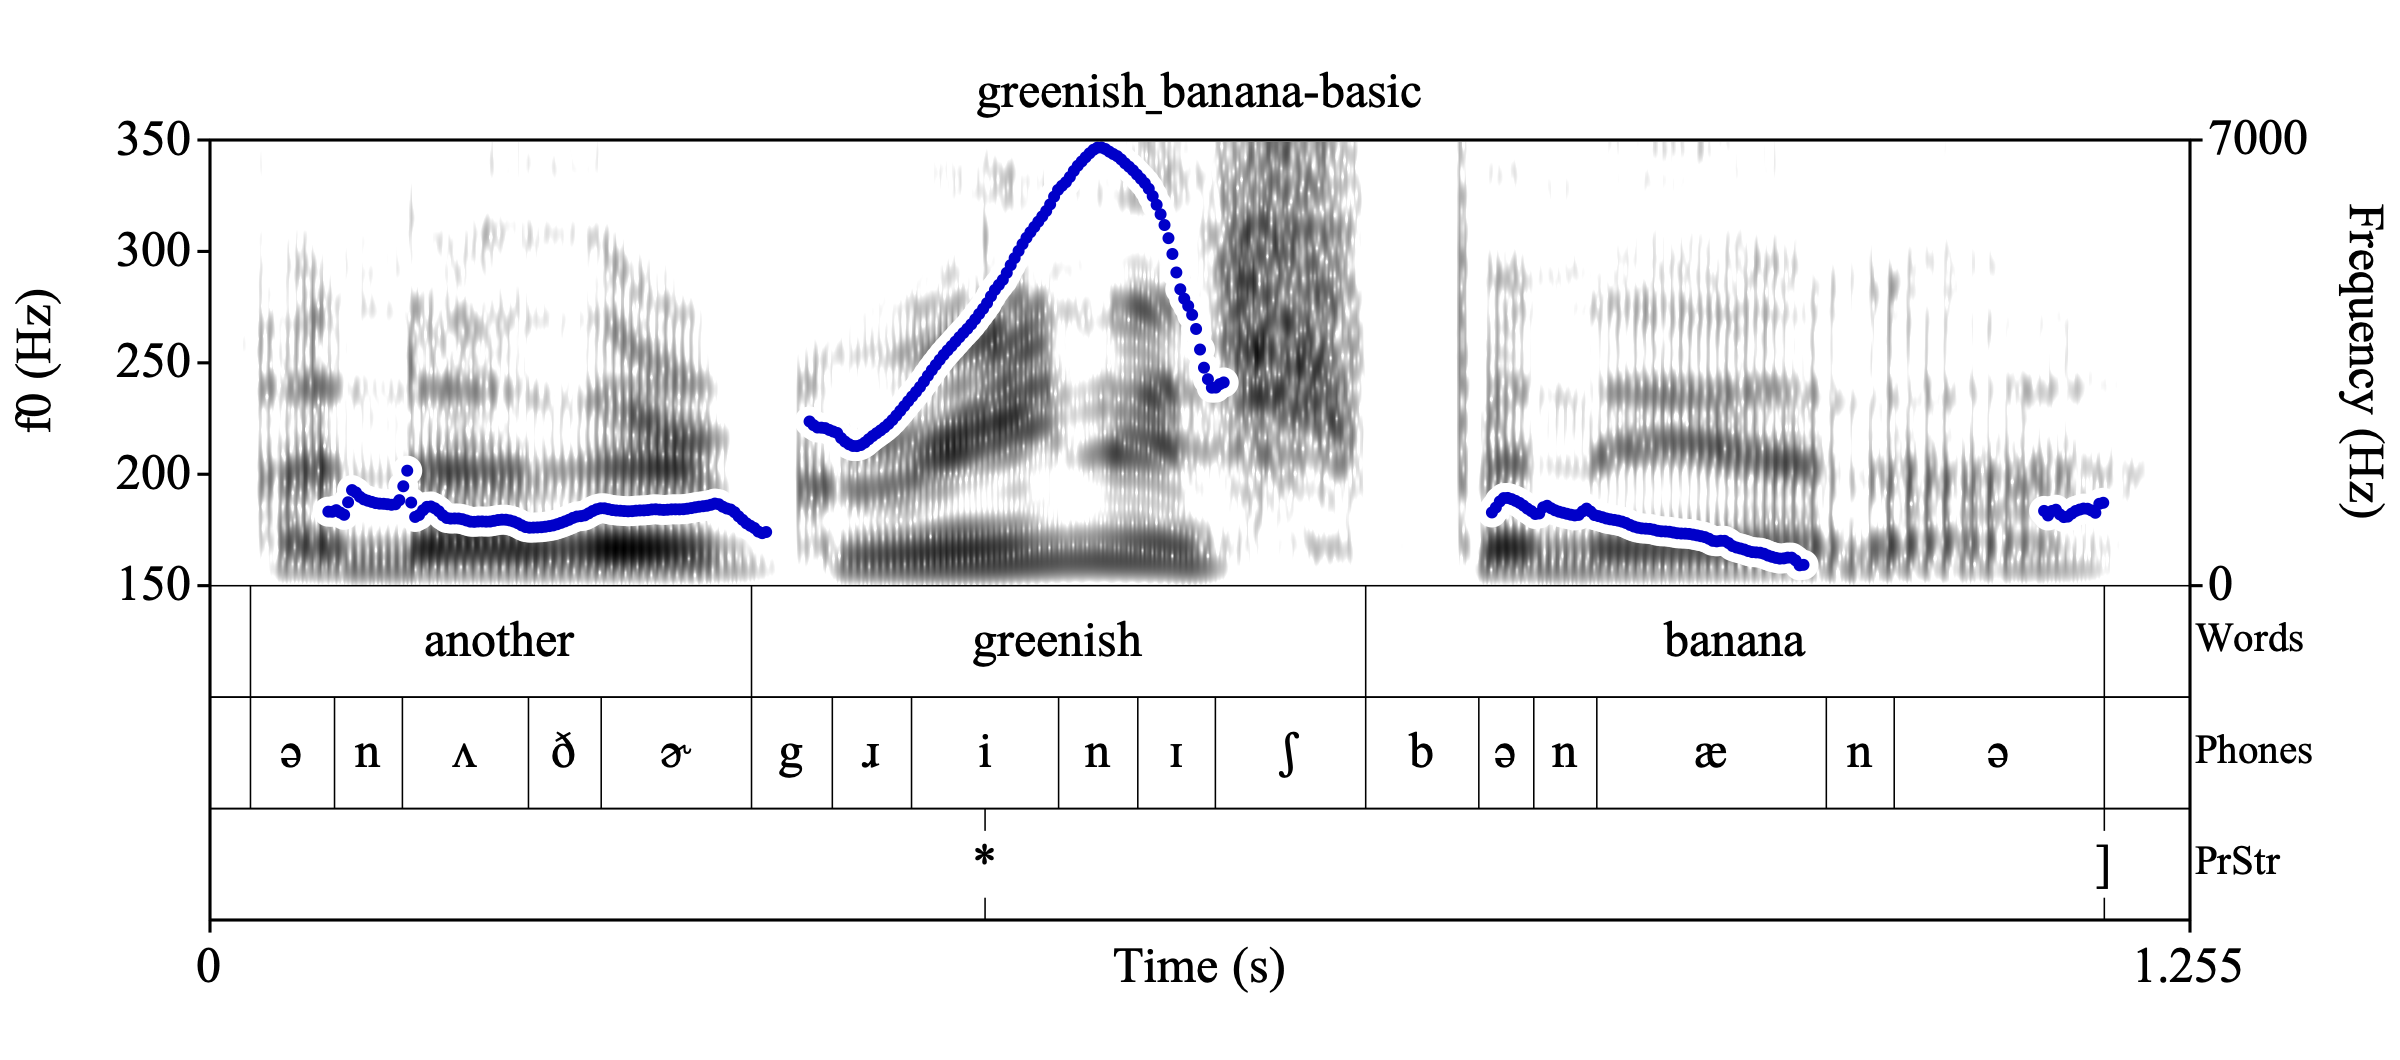
\includegraphics[width=.875\linewidth]{PrStr-greenish_banana-basic.png}
%
\caption{\texttt{greenish\_banana}: There is one prominent word, “greenish”.%
\label{fig:greenish banana prominent greenish}%
\index{Annotated example, PrStr tier (basic)!greenish\_banana}%
}
\end{figure}

\begin{figure}[H]
\centering
%
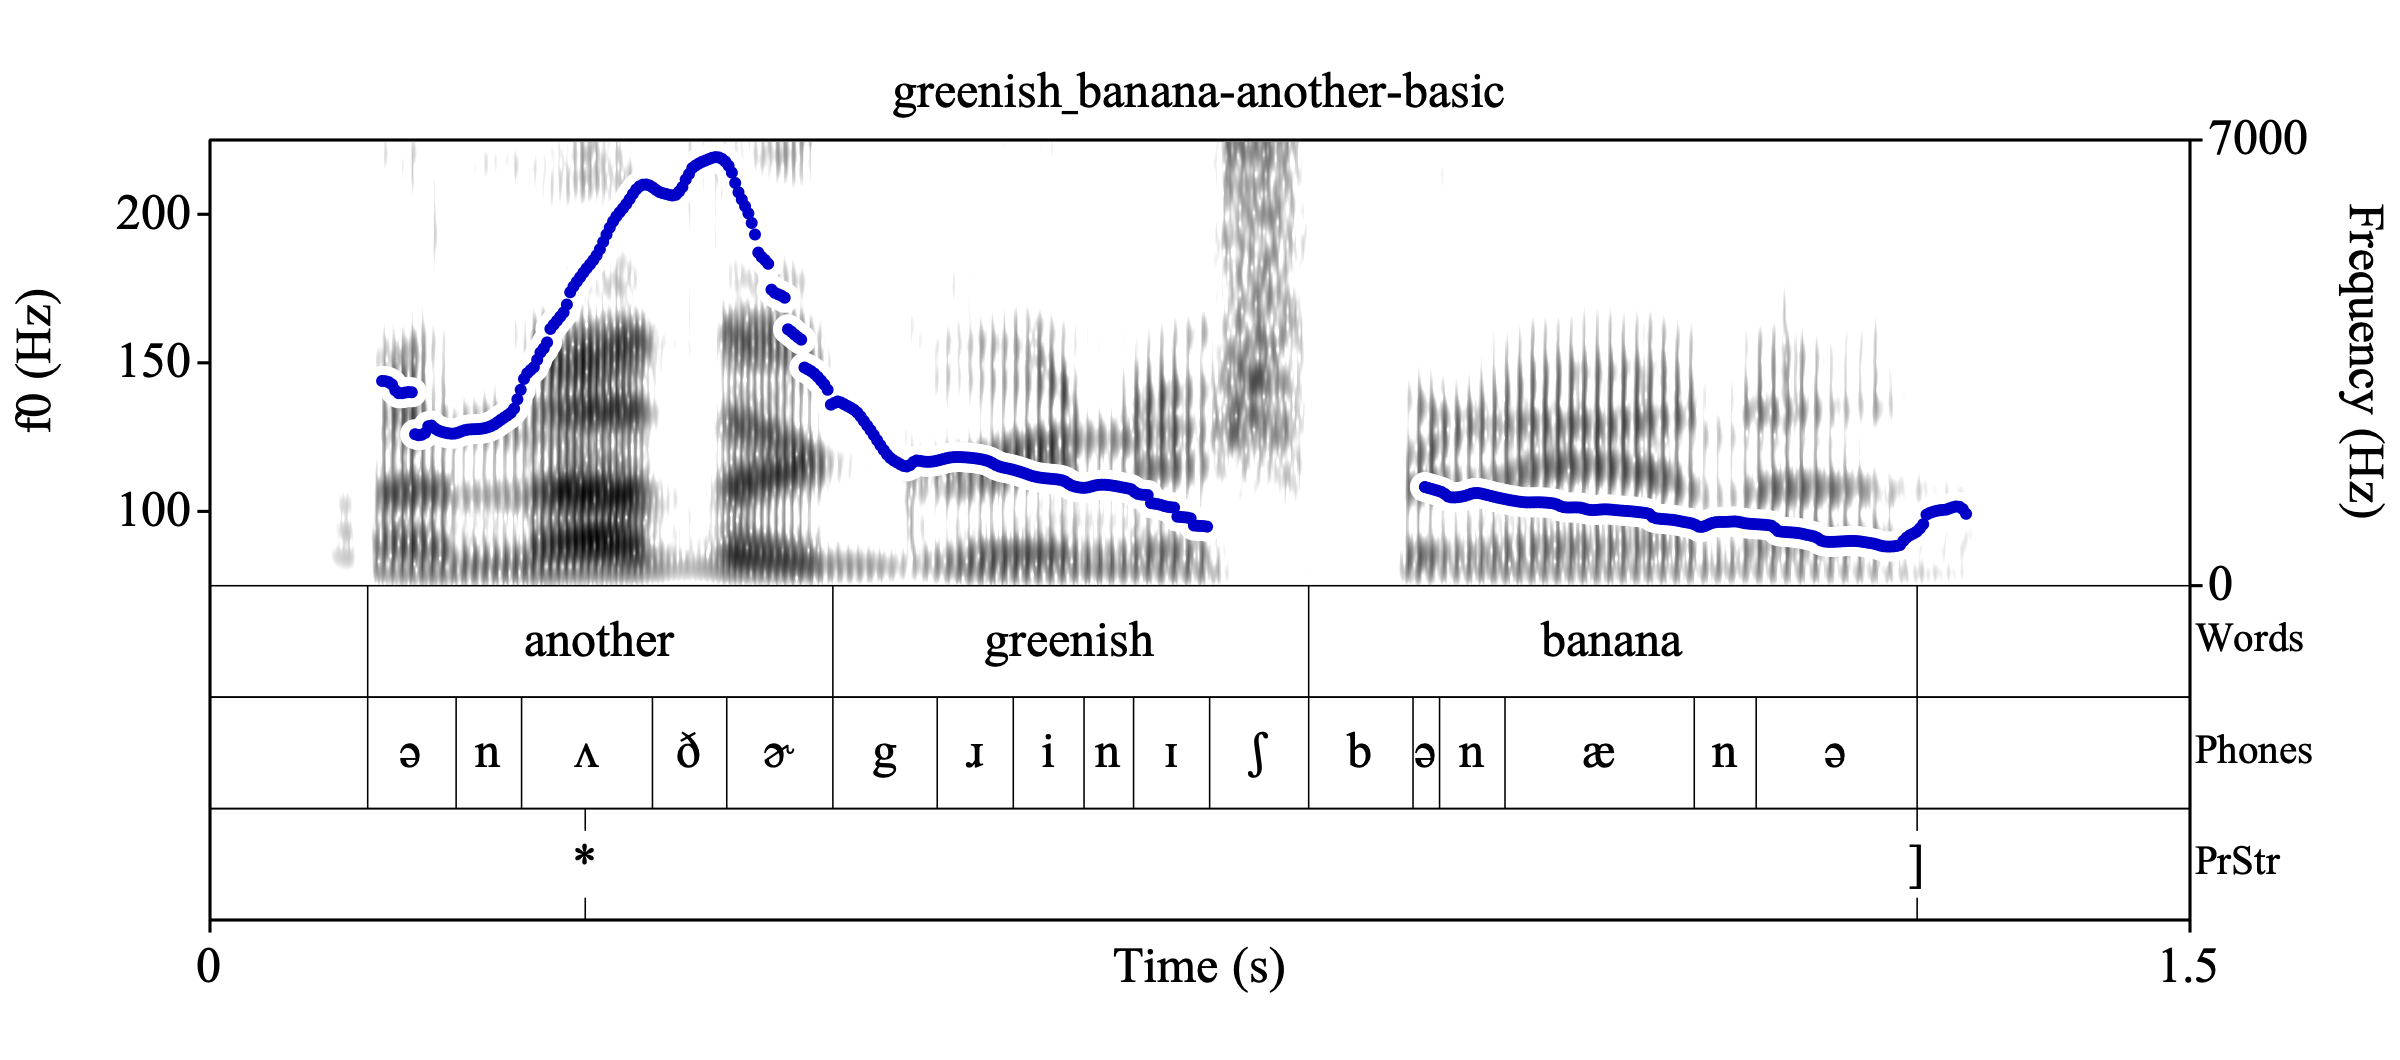
\includegraphics[width=.875\linewidth]{PrStr-greenish_banana-another-basic.png}
%
\caption{\texttt{greenish\_banana-another}: There is one prominent word, “another”.%
\label{fig:greenish banana prominent another}%
\index{Annotated example, PrStr tier (basic)!greenish\_banana-another}%
}
\end{figure}

\begin{infobox}[frametitle=\textbf{A NOTE ON PRAAT SETTINGS}]
If you follow along with these figures on your own machine using Praat (\citealt{praat}), there may be places where the figures in this monograph differ from the figures produced by your software. To minimize the number of differences, you can change the settings in your Praat to match those that are used to produce these figures. All figures in this monograph were created in Praat, using the “Draw Sound and TextGrid” functionality, which is a part of the PoLaR plugin for Praat. (\textit{This plugin can be found by going to \url{https://www.polarlabels.com}}.) This functionality is built on a script in which various settings related to pitch analysis and pitch display are specified – and these settings can radically affect how Praat identifies and analyzes pitch. These settings are given here: First, the Time Step analysis (found in \texttt{View>} Time step settings\ldots) was set to use a fixed strategy, at a time step of 0.0025s. Next, the “Advanced Pitch settings” (found in \texttt{Pitch>} Advanced pitch settings\ldots) were set as the following: Max. number of candidates=15, Very accurate=true, Silence threshold=0.03, Voicing threshold=0.5, Octave cost=0.05, Octave jump cost=0.5, and Voiced/Unvoiced cost=0.2. Screenshots of these settings windows are provided here: \par\begingroup\centering
	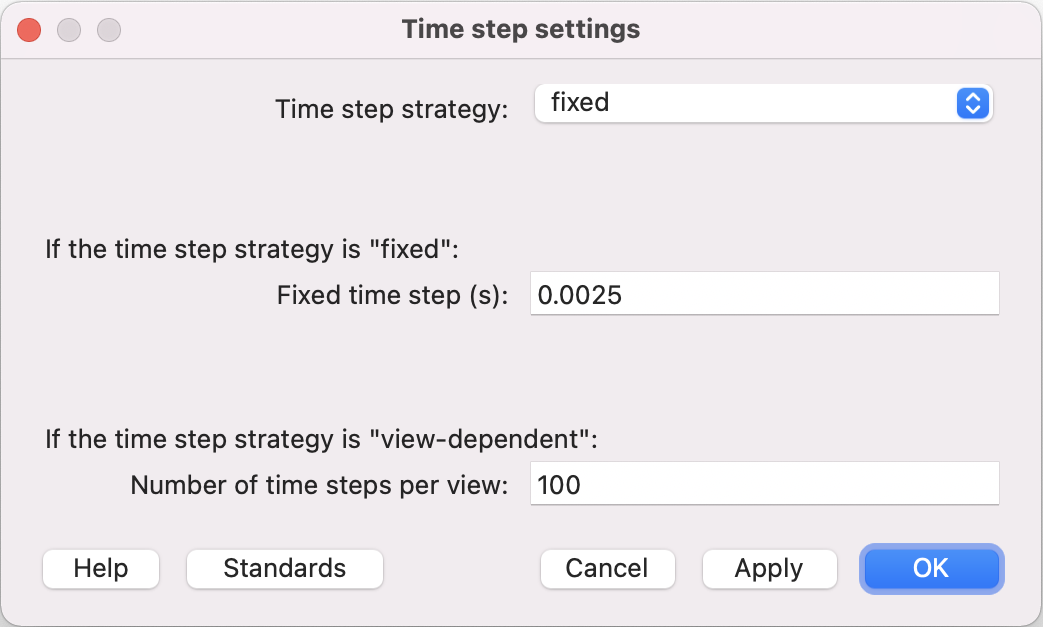
\includegraphics[width=.475\linewidth]{Praat-time-step-settings.png} 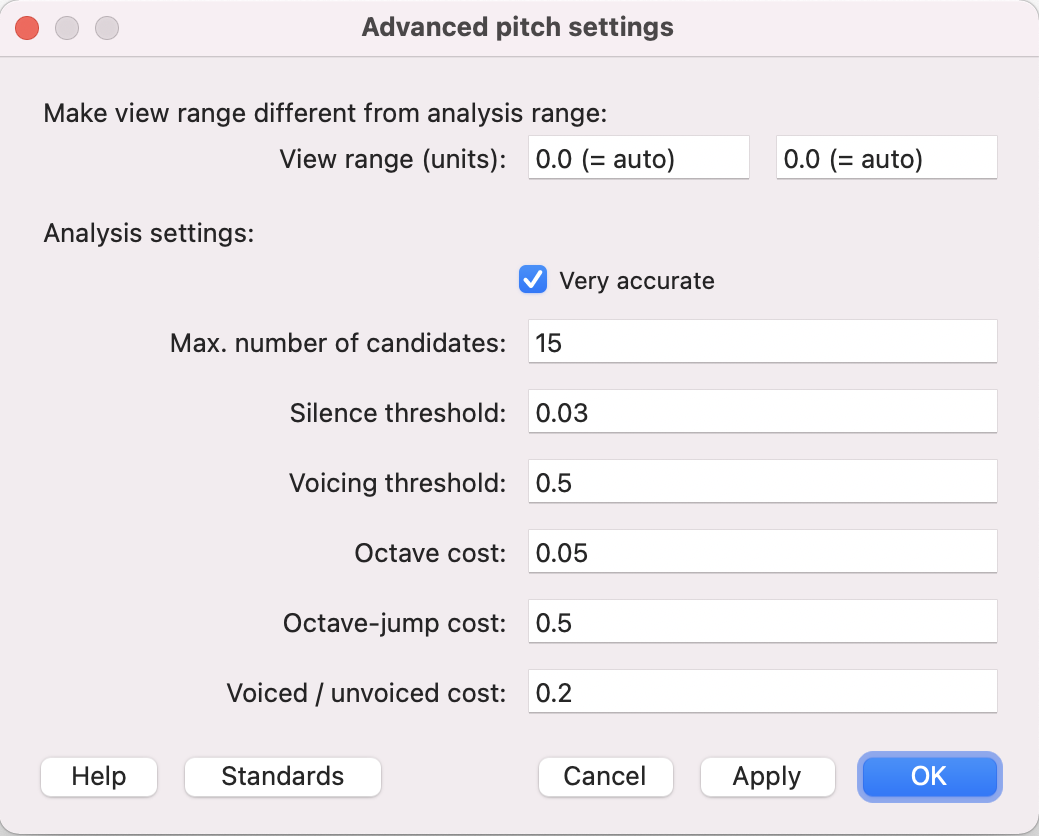
\includegraphics[width=.475\linewidth]{Praat-adv-pitch-settings.png} \par
	\endgroup (\textit{You may find it beneficial to adjust these settings further, to minimize pitch halving\slash doubling in particular recordings. However, doing so may result in pitch tracks that look different from the ones in this monograph.})
\label{note on praat settings}
\end{infobox}


It need not be the case that there is only one intonational prominence in an utterance; in fact, in many utterances with more than one content\footnote{So-called “content” words contrast with “function” words, where the former typically name concepts (e.g., “\langtext{human}”, “\langtext{energetic}”, “\langtext{remember}”) and the latter typically serve grammatical functions (e.g., “\langtext{the}”, “\langtext{itself}”, “\langtext{by}”, “\langtext{be}”).} word, it is common for there to be multiple words with intonational prominence. (There are plenty of examples of this throughout this monograph that show this, and more examples of PrStr labels are given in the “examples” section below.)

To annotate intonational prominence, we will adopt the \textlabel{*} symbol, from the AM tradition. In English, like lexical stress, intonational prominence is a phonological property associated with \textit{a syllable}, and so when we use the \textlabel{*} annotation, we want to align it in the Praat TextGrid with respect to the syllable that is perceived as prominent.\footnote{Prominence is realized with a number of acoustic cues, which may include increased amplitude, increased duration, one or more pitch movements, and hyperarticulation. At the same time, it is not the case that all of these cues are present for any given prominence. Moreover, across different contexts, any member of the set of cues may be weighted differently in their effect on perception of prominence. Finally, these cues only signal the intonational prominence and are not the intonational prominence itself. As such, instead of requiring that a PrStr tier labeller attend carefully to the cues (though they can!), PoLaR only requires that listeners consult their intuition that they perceive a given syllable as intonationally prominent.\label{fn:prominence cues}} This is shown in Figures \ref{fig:greenish banana prominent greenish} and \ref{fig:greenish banana prominent another}, on the third tier.

NOTE: Labellers are encouraged to adhere to consistent practices for the time-alignment of the \textlabel{*} labels. As an example of a regular practice for time-alignment, the present authors time-align their \textlabel{*} labels to the middle of (the segment that the forced aligner picks out as) the vowel\footnote{More accurately, we mean the middle of the “nucleus”, which is often realized as a vowel in English, but can also be realized as certain syllabic consonants (e.g., [n̩]).} of the syllable that is perceived as the intonationally prominent.\footnote{For a vast majority of cases, this syllable is the lexically stressed syllable of a word that is perceived as prominent – but not always (cf. certain cases of focus such as what is called “metalinguistic focus” in \citealt{erteschik-shir99} \textit{et seqq}, as well as other cases where contrastive focus can be found on other syllables as discussed in \citealt{armstrongschwenter16} and \citealt{ahn-21a}).}

Let’s now turn to prosodic phrasing. Phrasing refers to how words are grouped, so that some are perceived with no disjuncture between them (i.e., they are perceived as sounding closely grouped together), and some words are perceived as having (various levels of) disjuncture between them. Though pauses between words are one very strong cue to disjuncture, disjuncture is \uline{not} the same as pauses. (It can occur when there is no discernible pause between words, too.) Consider the following example, in which there is a perceived phrase boundary between “\langtext{beans}” and “\langtext{some}”, despite the fact that the /z/ sound at the end of “\langtext{beans}” leads right into the /s/ sound of “\langtext{some}”, with no pause:\footnote{Like prominence (see footnote \ref{fn:prominence cues}), phrase boundaries can be realized with a number of different acoustic cues. Cues to phrase boundaries may include a pause between phrases, changes in rate of speech production at the end of a phrase (and beginning of the next one), hyperarticulation at the beginning of a phrase, one or more pitch movements, changes in pitch range, and changes in voice quality. At the same time, it is not the case that all of these cues are present for any given phrase boundary. Moreover, across different contexts, any member of the set may be weighted differently in their effect on perception of phrase boundaries. Again, a PrStr tier labeller need not attend carefully to the particular acoustic cues (though they can!); instead, PoLaR only requires that listeners consult their intuition that they perceive a sense of disjuncture.\label{fn:phrasing cues}}

\begin{figure}[H]
\centering
%
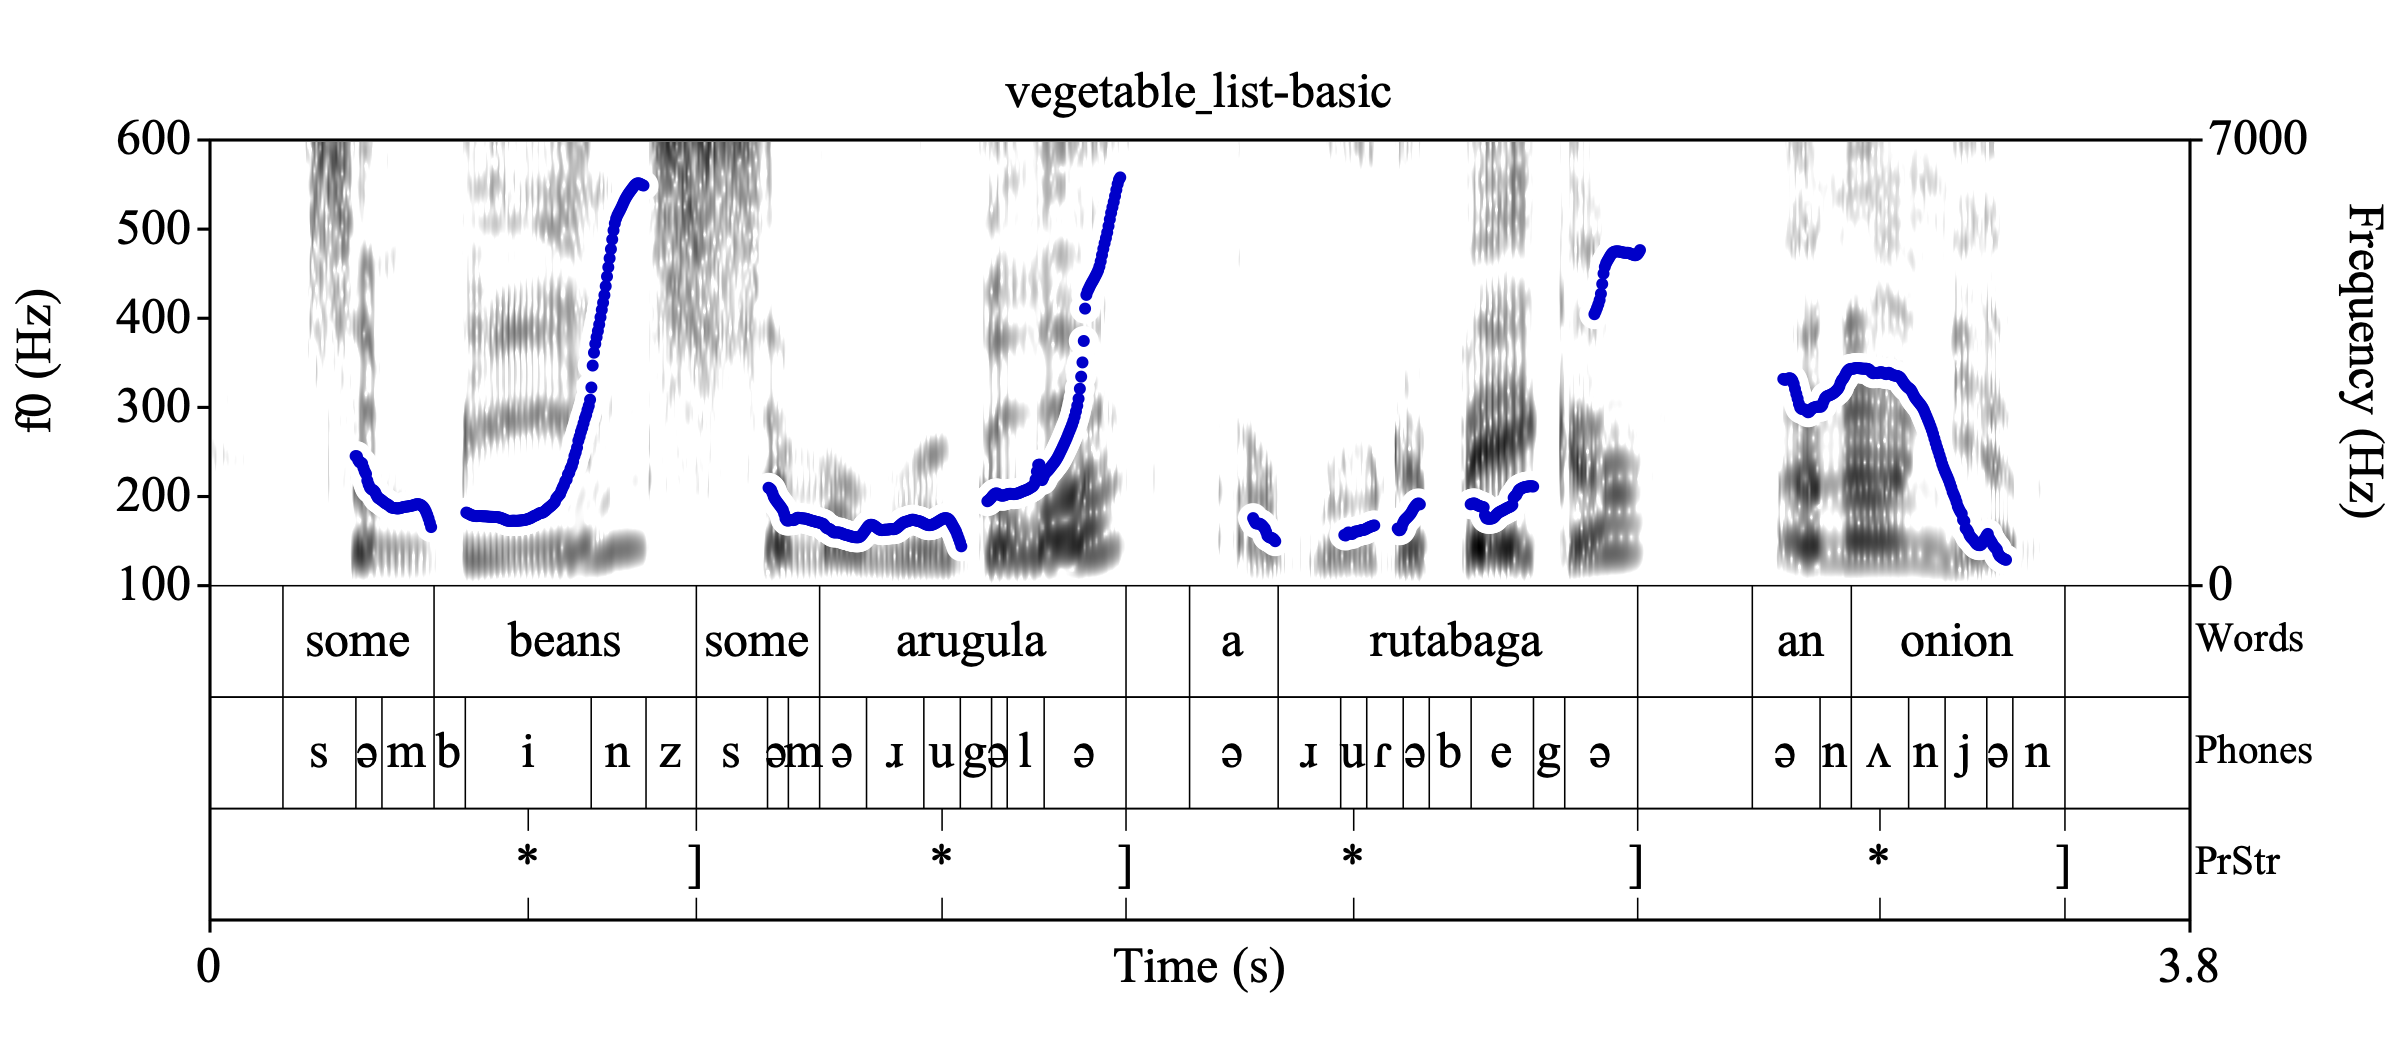
\includegraphics[width=.875\linewidth]{PrStr-vegetable_list-basic.png}
%
\caption{\texttt{vegetable\_list}: There are four prosodic phrases.%
\label{fig:vegetable list phrases}%
\index{Annotated example, PrStr tier (basic)!vegetable\_list}%
}
\end{figure}

Prosodic phrasing (like prominence) cannot be predicted solely on the basis of the words alone, but requires more knowledge about the context in which those words were spoken. In the example above, it is read as a list of four items, in four phrases; but you could imagine a context where the speaker was listing all the words on a page and then pronounces it as eight separate phrases (one for each word). Because phrasing is variable in this way (and because it has important effects on various suprasegmental properties), we annotate phrase boundaries explicitly.

To annotate prosodic phrasing in English, we will adopt the convention from the AM tradition of only annotating the boundary at the end of a phrase. (The idea is that the end of one phrase coincides with the beginning of another.\footnote{This is not a given for all work on prosodic phonology. As such, in the Advanced labels chapter, we describe a means of labelling other boundary edges.}) We will use the \textlabel{]} symbol for this. The end of a phrase is typically aligned with the end of a word, and so when we use the \textlabel{]} annotation, we want to align it in the Praat TextGrid with respect to the word boundary of the phrase-final word. Refer to the third tier of the Figure \ref{fig:vegetable list phrases}, to see this. Because basic PoLaR labels only indicate where a phrase ends, in cases where there is a pause after a phrase (e.g., after “\langtext{arugula}” or “\langtext{rutabaga}” in Figure \ref{fig:vegetable list phrases}), the \textlabel{]} label is placed before the pause. (Again, for more examples of this PrStr labelling, more examples are given throughout this monograph and in the “examples” section below.)

\subsubsection{Prosodic Structure Transcription}
To summarize, the two labels we have seen so far are described in Table \ref{2 PrStr basic labels}.

\begin{longtable}{cll} \toprule \textbf{Label} & \textbf{Phonological Object} & \textbf{Label is time-aligned with \_\_\_\_\_}\tabularnewline
\midrule \endhead
\textlabel{*} & Prominence & A syllable that has intonational prominence \tabularnewline
\textlabel{]} & Phrase’s Right Edge & The right edge of the final word of a phrase \tabularnewline
\bottomrule 
\caption{Two Basic labels for the Prosodic Structure tier (for English).%
\label{2 PrStr basic labels}%
}
\end{longtable}

(\textit{For labellers who wish to annotate more fine-grained levels of phonological analysis,}\footnote{For example: different types of prominence (nuclear stress, pre-\slash post-nuclear stress, focal stress, etc.), and different types of phrases (intermediate\slash phonological phrases, intonational phrases, etc.) or different phrase edges (i.e., the left edge of a phrase).} \textit{there are optional Advanced labels for this tier as well, which are described in Chapter \ref{ch:advanced}.})

\begin{infobox}[frametitle=\textbf{A side-note about this tier}]
This tier is called “Prosodic Structure”, and contains labels that refer to elements of that structure that are relevant for intonational annotation. There is more to prosodic structure than has been described here; e.g., the labels described until now do not annotate lower levels of structure (e.g., syllable structure, lexical prominence, etc.) nor do they differentiate between different levels of intonational prominence or prosodic phrasing. In this way, the labels we have laid out here are designed to \textbf{reflect \uline{certain particular assumptions} about the intonational phonology and prosodic structures of English}: i.e., that the core elements of English intonational phonology are syllables with post-lexical prominence (motivating the \textlabel{*} label) and the right edges of phonological phrases (motivating the \textlabel{]} label). Because prosodic structure consists of a superset of these features that are relevant for intonation that we annotate here, PoLaR is flexible enough that this set of labels can be augmented or changed, to fit the needs\slash views of the labeller. (For some examples, see Section \ref{sec:prstr-advanced} of Chapter \ref{ch:advanced}, as well as all of Chapter \ref{ch:beyond}.) Whenever labellers deviate from this set, they will need to describe the labels they use and what they are used for.
\end{infobox}

As a reminder, PrStr labelling can be done solely on the basis of labeller perception, without any attention paid to particulars of the acoustic signal. For example, pitch changes may be cues to prominence or phrasing, but labellers need not be looking at a pitch track when annotating for PrStr. (This is beneficial since software-based pitch tracking is sometimes unreliable.\footnote{More will be said on unreliable pitch tracks in Section \ref{sec:intonational-contours-and-software-based-pitch-tracks}.}) In fact, the labeller could provide PrStr tier annotations without any spectrogram, f0 curve, or other visualization of the acoustics – indeed people can indicate the location of prominence and boundaries without any familiarity with prosody. In fact, experimental work using RPT methodologies (\citealt{cole-14, cole-17}, \citealt{cole-16}) have demonstrated that naive listeners can reliably identify prominent words (i.e., those that “stand out”) and phrasing boundaries (i.e., where adjacent words “belong to different chunks”).

\subsubsection{Labeller Uncertainty}\label{sec:labeller-uncertainty}

It is not always a straightforward task to decidedly determine whether a word contains a prominence, or whether or not two words are separated by a phrase boundary. (This has to do with the fact that there is no single cue to prominence or phrasing that is deterministic; instead, networks of cues contribute to indicating these properties. See footnotes \ref{fn:prominence cues} and \ref{fn:phrasing cues}.) Some key elements that may lead to labeller uncertainty are an ambiguous signal (i.e., a signal that is, at least on some dimensions, consistent with several different prosodic representations) and/or a diminished set of cues to prominence or phrasing (i.e., below some threshold of cues that makes detecting prominence or phrasing straightforward). Examples of the sort of signal that may be difficult to label prosodic structure for might include cases of extremely reduced pitch range, quiet speech, very rapid or very slow speech, speech with little intonational variation, and/or disfluent speech, among many other possibilities.

As a first case of uncertainty, a labeller may wish to indicate uncertainty about whether a particular item is prominent. In these cases, the labeller can add a ‘\textlabel{?}’ to the prominence label, creating the ‘\textlabel{?*}’ label. For example, in \texttt{menu\_eleven}, the labeller is uncertain about which, if any, of the first four words are prominent:

\begin{figure}[H]
\centering
%
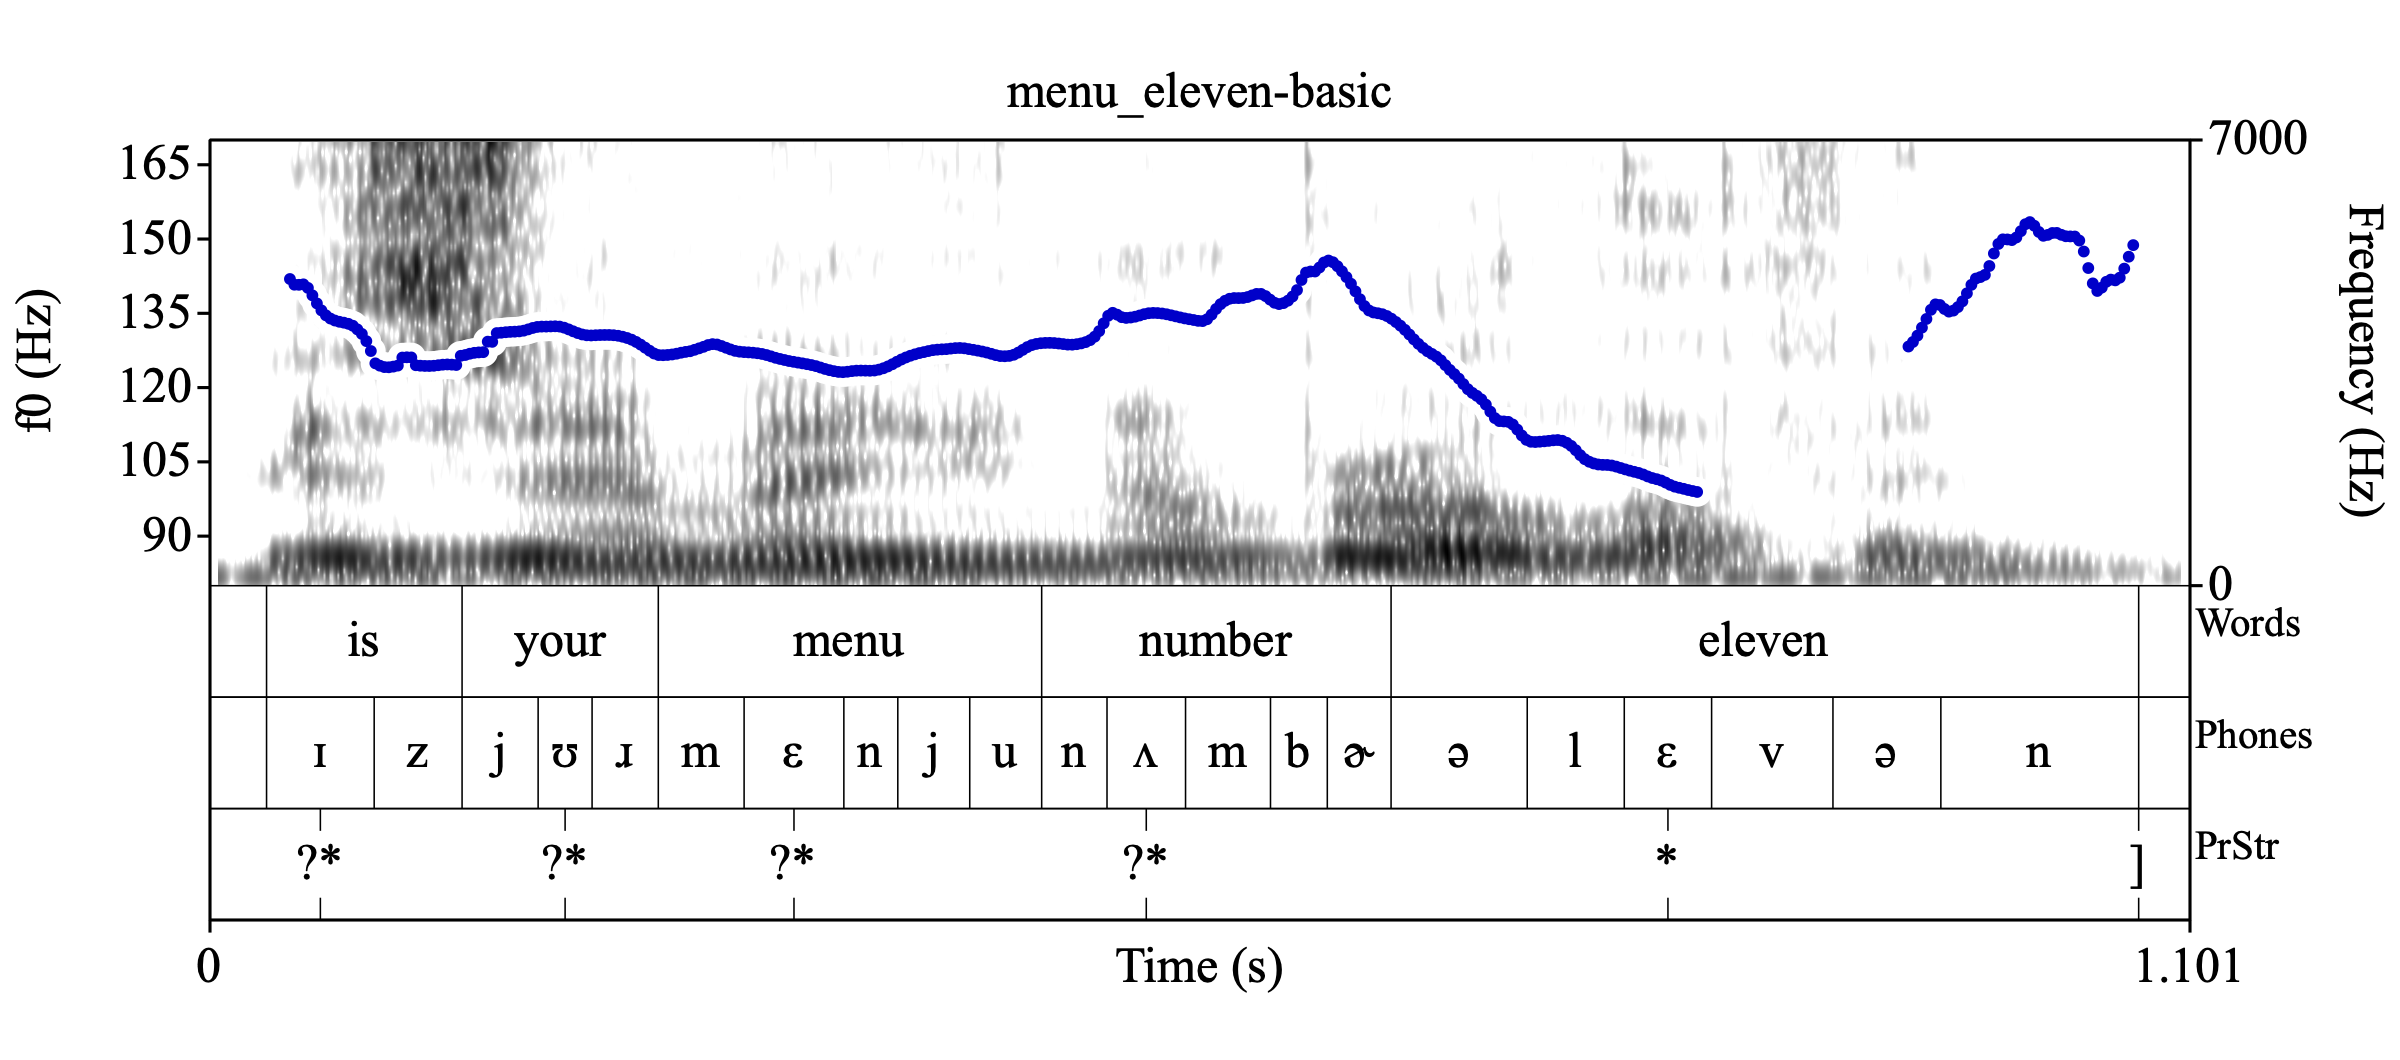
\includegraphics[width=.875\linewidth]{PrStr-menu_eleven-basic.png}
%
\caption{\texttt{menu\_eleven}: The labeller is uncertain as to whether any of the first four words are prominent or not.%
\label{fig:menu eleven PrStr uncertainty}%
\index{Annotated example, PrStr tier!menu\_eleven}
}
\end{figure}

Additional cases illustrating labeller uncertainty are provided in the Advanced PoLaR labels chapter.

Similar to uncertainty labels for prominence, a labeller can indicate uncertainty about the presence of a phrase boundary using the ‘\textlabel{?]}’ label. For example, in \texttt{librivox-zip1}, the labeller is uncertain of whether there is a phrase boundary between “\langtext{Librivox}” and “\langtext{recording}”:

\begin{figure}[H]
\centering
%
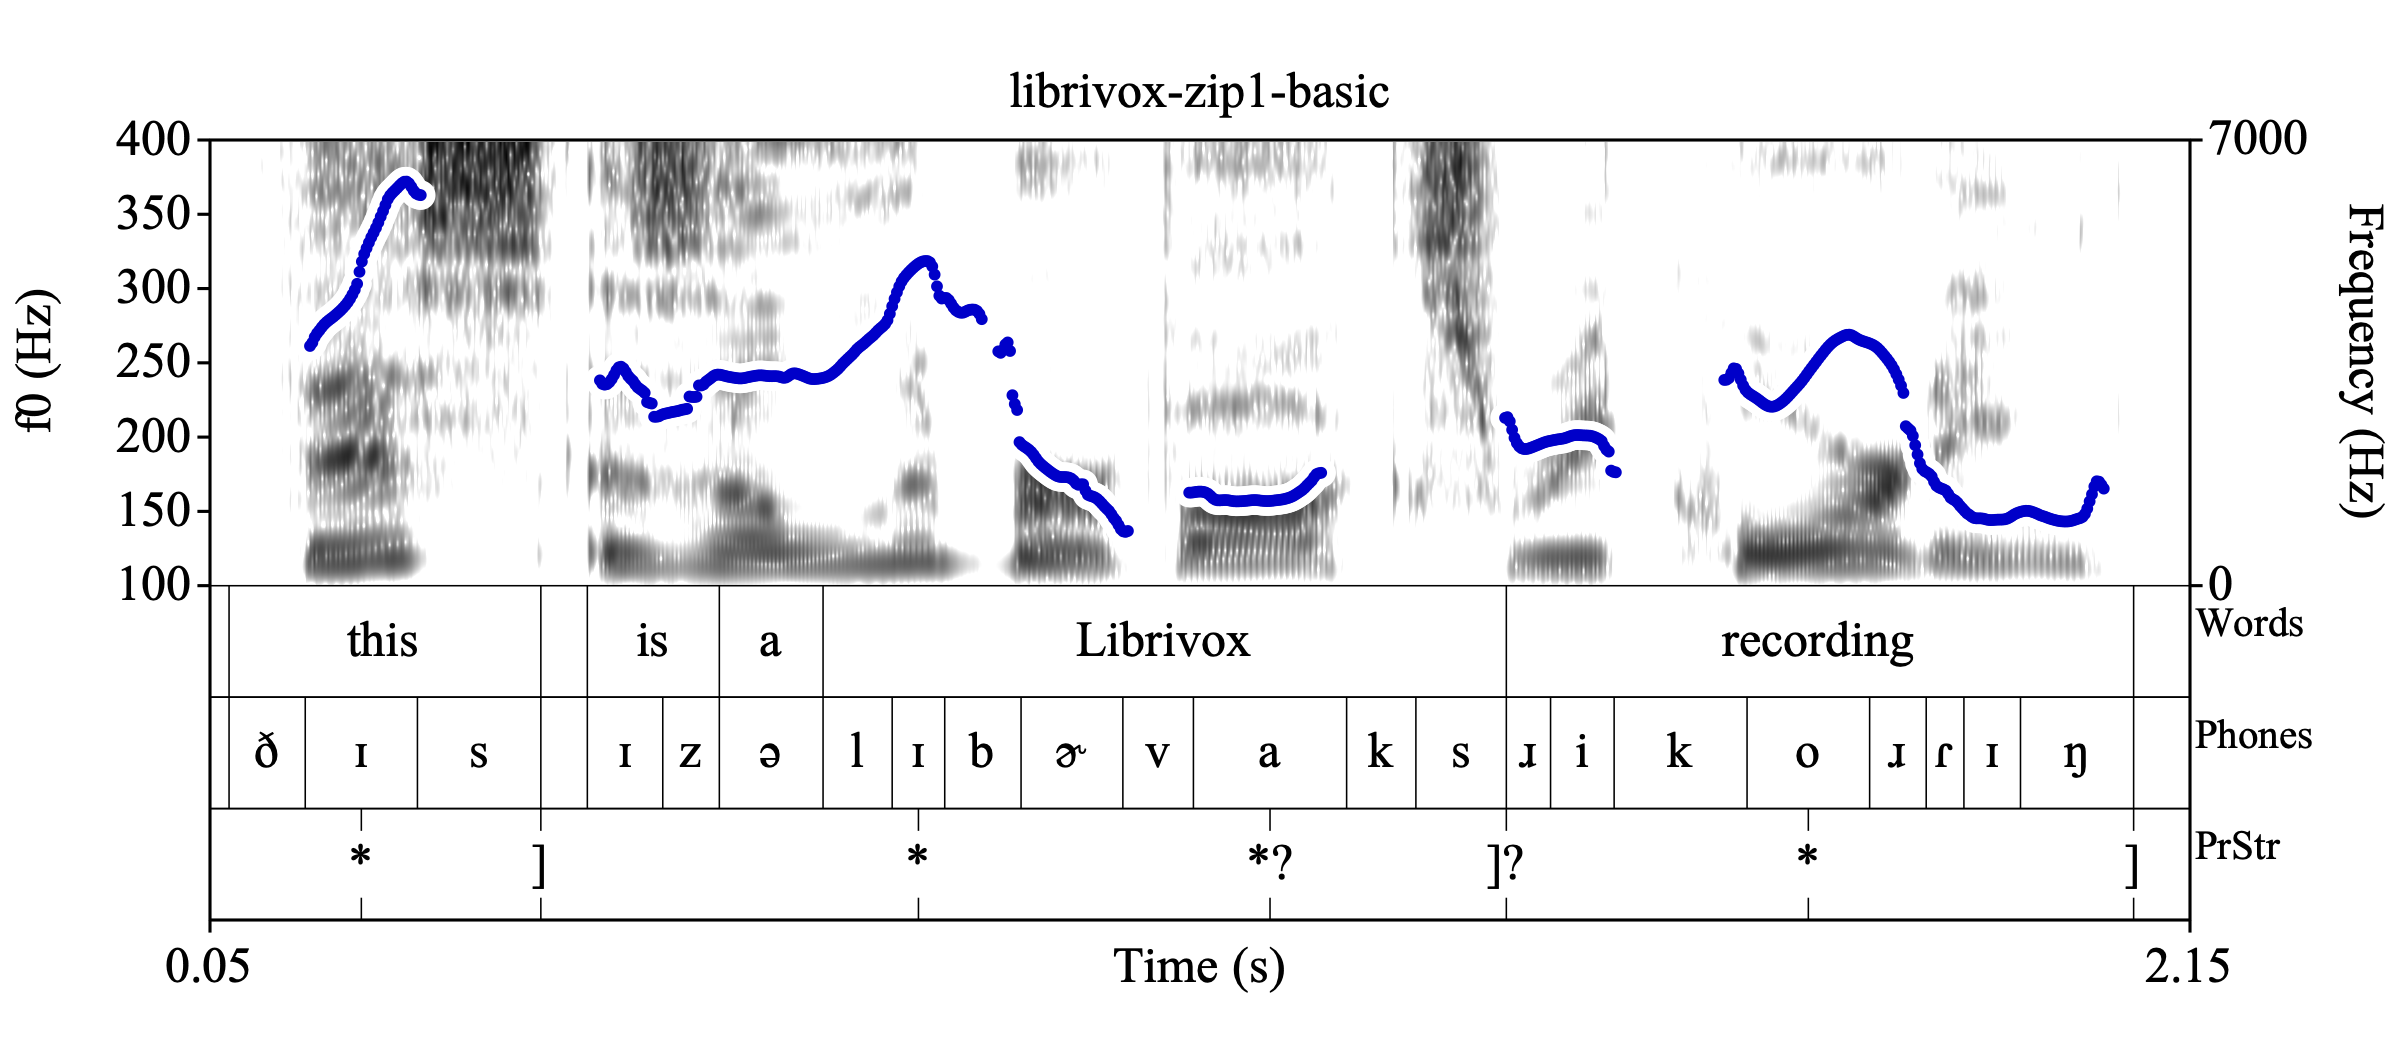
\includegraphics[width=.875\linewidth]{PrStr-librivox-zip1-basic.png}
%
\caption{\texttt{librivox-zip1}: The labeller is uncertain as to whether there is a prosodic phrase boundary between ‘Librivox’ and ‘recording’.%
\label{fig:librivox-zip1 PrStr uncertainty}%
\index{Annotated example, PrStr tier!librivox-zip1}
}
\end{figure}

(Note that there is also a \textlabel{?*} on the final syllable of “\langtext{Librivox}”.) Again, additional cases of labeller uncertainty are provided in chapter \ref{ch:advanced}.

Explicitly annotating uncertainty may be useful for future analysis of which cues local to \textlabel{*} and \textlabel{]} labels are reliably informative to a labeller regarding the presence of prominence and phrasing, and what sorts of acoustics lead to labeller uncertainty, as well as for studies of individual differences in cue interpretation. Additionally, an experienced labeller may have intuitions about why they are uncertain about the existence of prominence\slash phrasing; in such cases, the labeller is encouraged to annotate these intuitions on a “miscellaneous” tier.\footnote{This is because, though some cues to prominence and phrasing are annotated elsewhere (e.g., the Points and Ranges tiers), it can be helpful for future readers of labels if the labeller includes more explicit information about what led the labeller to be uncertain. (This may be especially helpful for coming to consensus labels, when multiple labellers PoLaR-annotate the same file.)}

\subsubsection{Examples of Basic Prosodic Structure labels}\label{sec:more-examples}

In this section you will find additional figures, showing audio examples labelled with PrStr labels. The name of each sound file is provided in the caption for each figure, and those sound files (and corresponding TextGrids) can be found at \url{https://www.polarlabels.com}. These figures show the words, the phones, and the PrStr labels. In some cases, MAE\_ToBI Tones labels\footnote{The alignment of the ToBI Tones tier labels follows \citealt{beckman-05} (p.25), where it is stated that pitch accent labels should be timed within the accented syllable, in such a way that it is nearest to the appropriate f0 minimum\slash maximum. Some laboratories prefer that pitch accent labels (on ToBI Tones tier) be time-aligned to occur within the stressed syllable’s nucleus (as was the guidance in earlier ToBI materials; e.g., \citealt{beckmanhirschberg94}).} are given alongside PrStr labels for comparison; but readers of these annotations do \uline{not} need to understand MAE\_ToBI to continue on with PoLaR.\footnote{Note that, by design, PrStr labels (on their own) encode less information than ToBI Tones labels.} The original TextGrid files used to produce these figures have additional annotation, with other PoLaR tiers.

\paragraph{Basic PrStr Examples 1 and 2: differences in edge tones}

The following examples share the same words and prominence locations but differ in how the speaker chooses to vary the f0 to mark the phrase edge tones. In PoLaR, these final boundaries would both be marked with the \textlabel{]} symbol and the acoustic distinction will be annotated in other tiers (e.g., in the Points Tier, as discussed in the next section, §\ref{sec:points}). For those familiar with ToBI labels, which we have included in these examples, note that the f0 contrast (falling to a low vs rising f0) and the prosodic function (disjuncture) labels are bundled together. 

\begin{figure}[H]
\centering
%
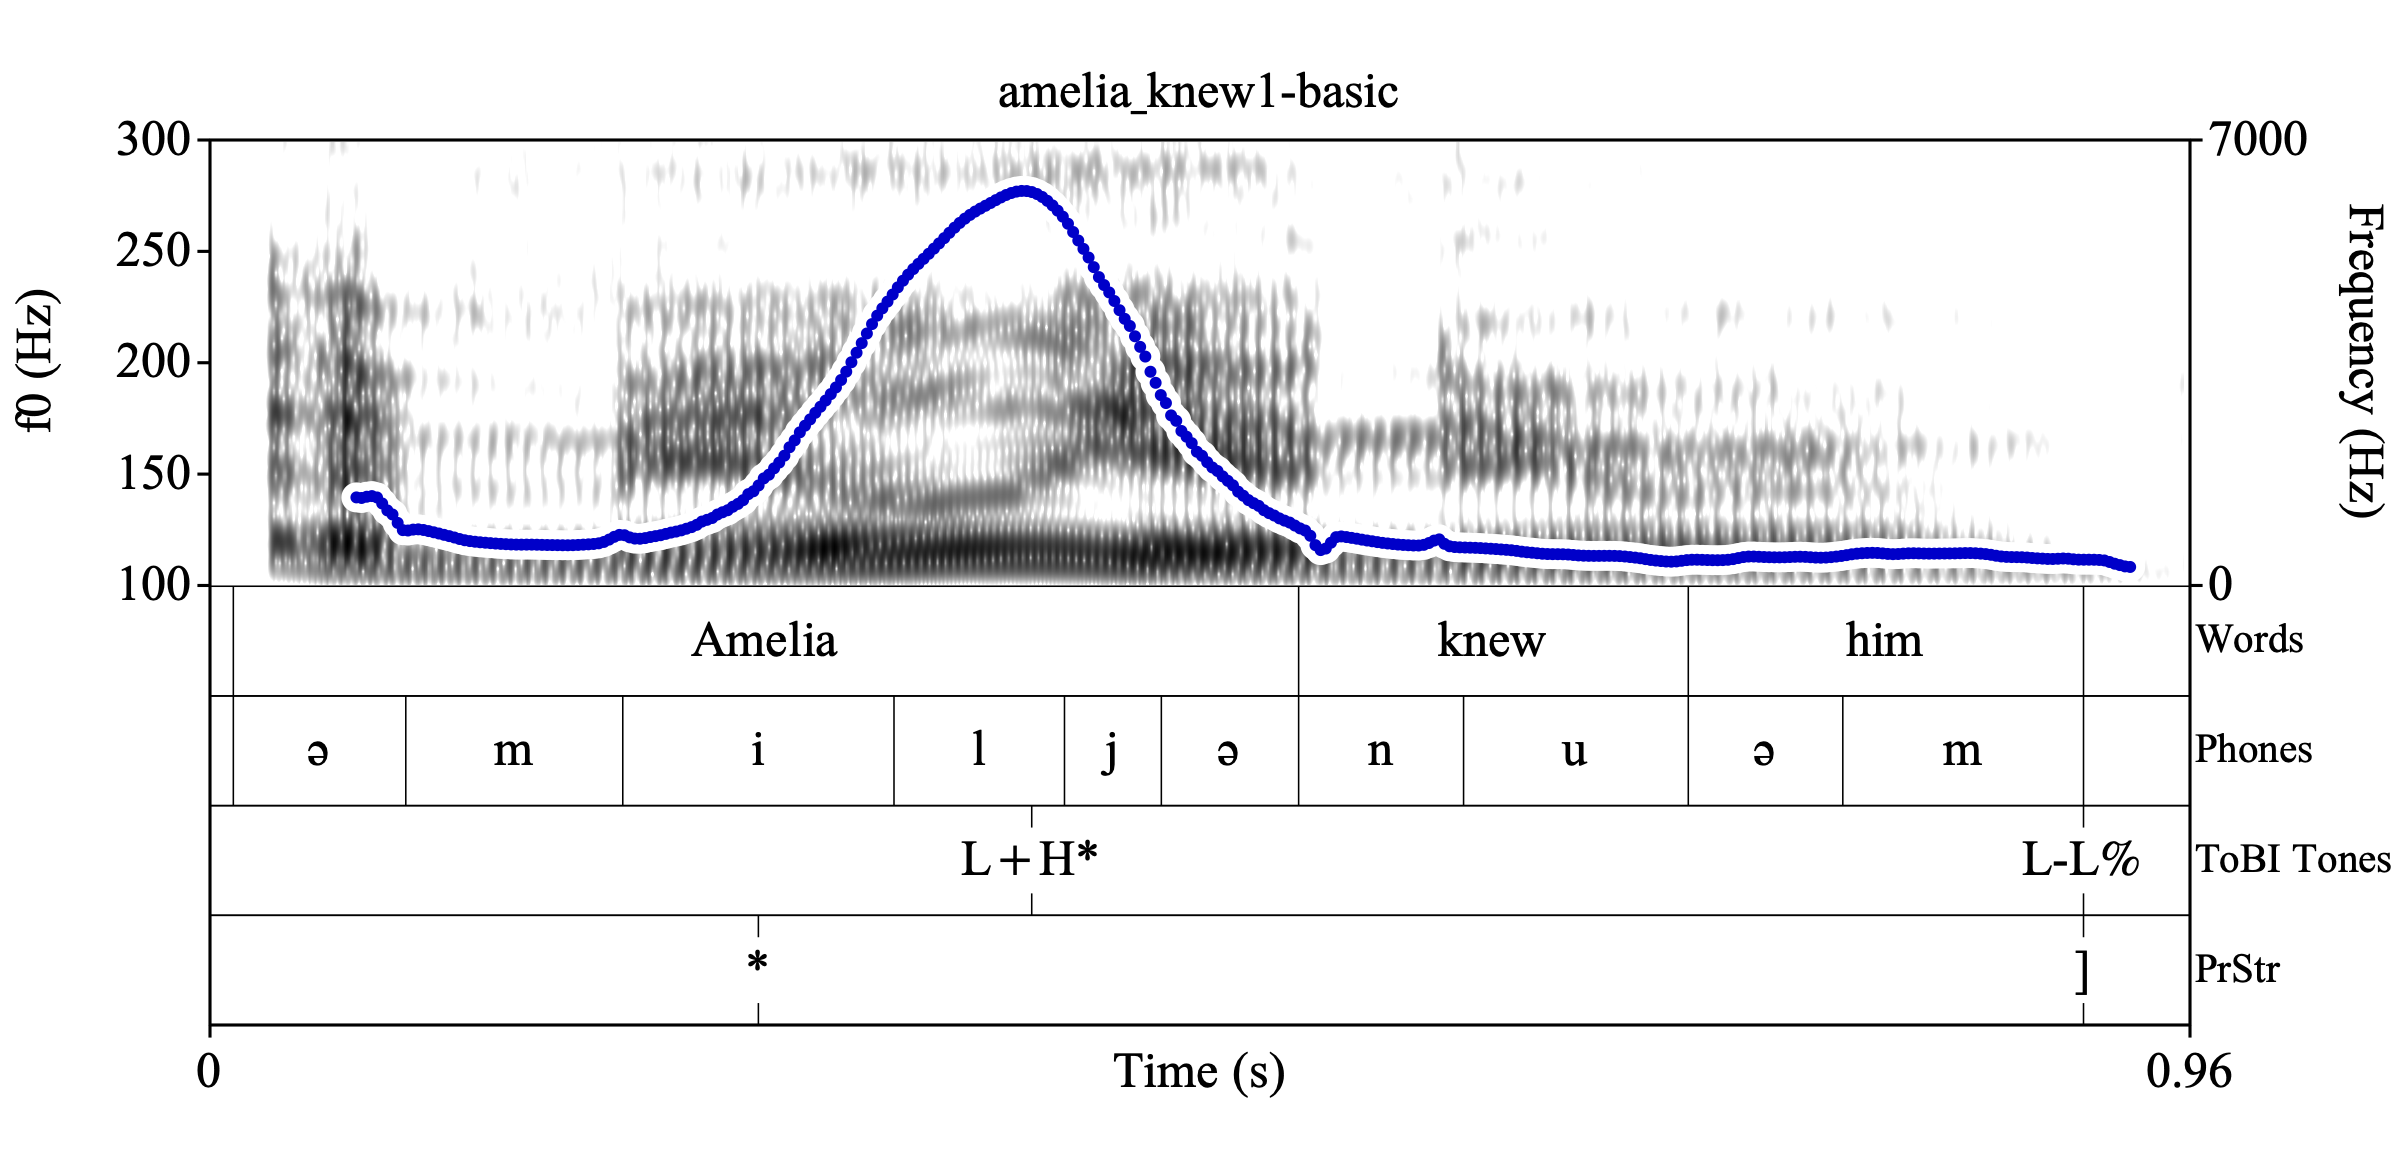
\includegraphics[width=.875\linewidth]{PrStr-amelia_knew1-basic.png}
%
\caption{\texttt{amelia-knew1}, with the PrStr tier annotated.%
\label{fig:amelia-knew1 PrStr}%
\index{Annotated example, PrStr tier (basic)!amelia-knew1}%
}
\end{figure}

\begin{figure}[H]
\centering
%
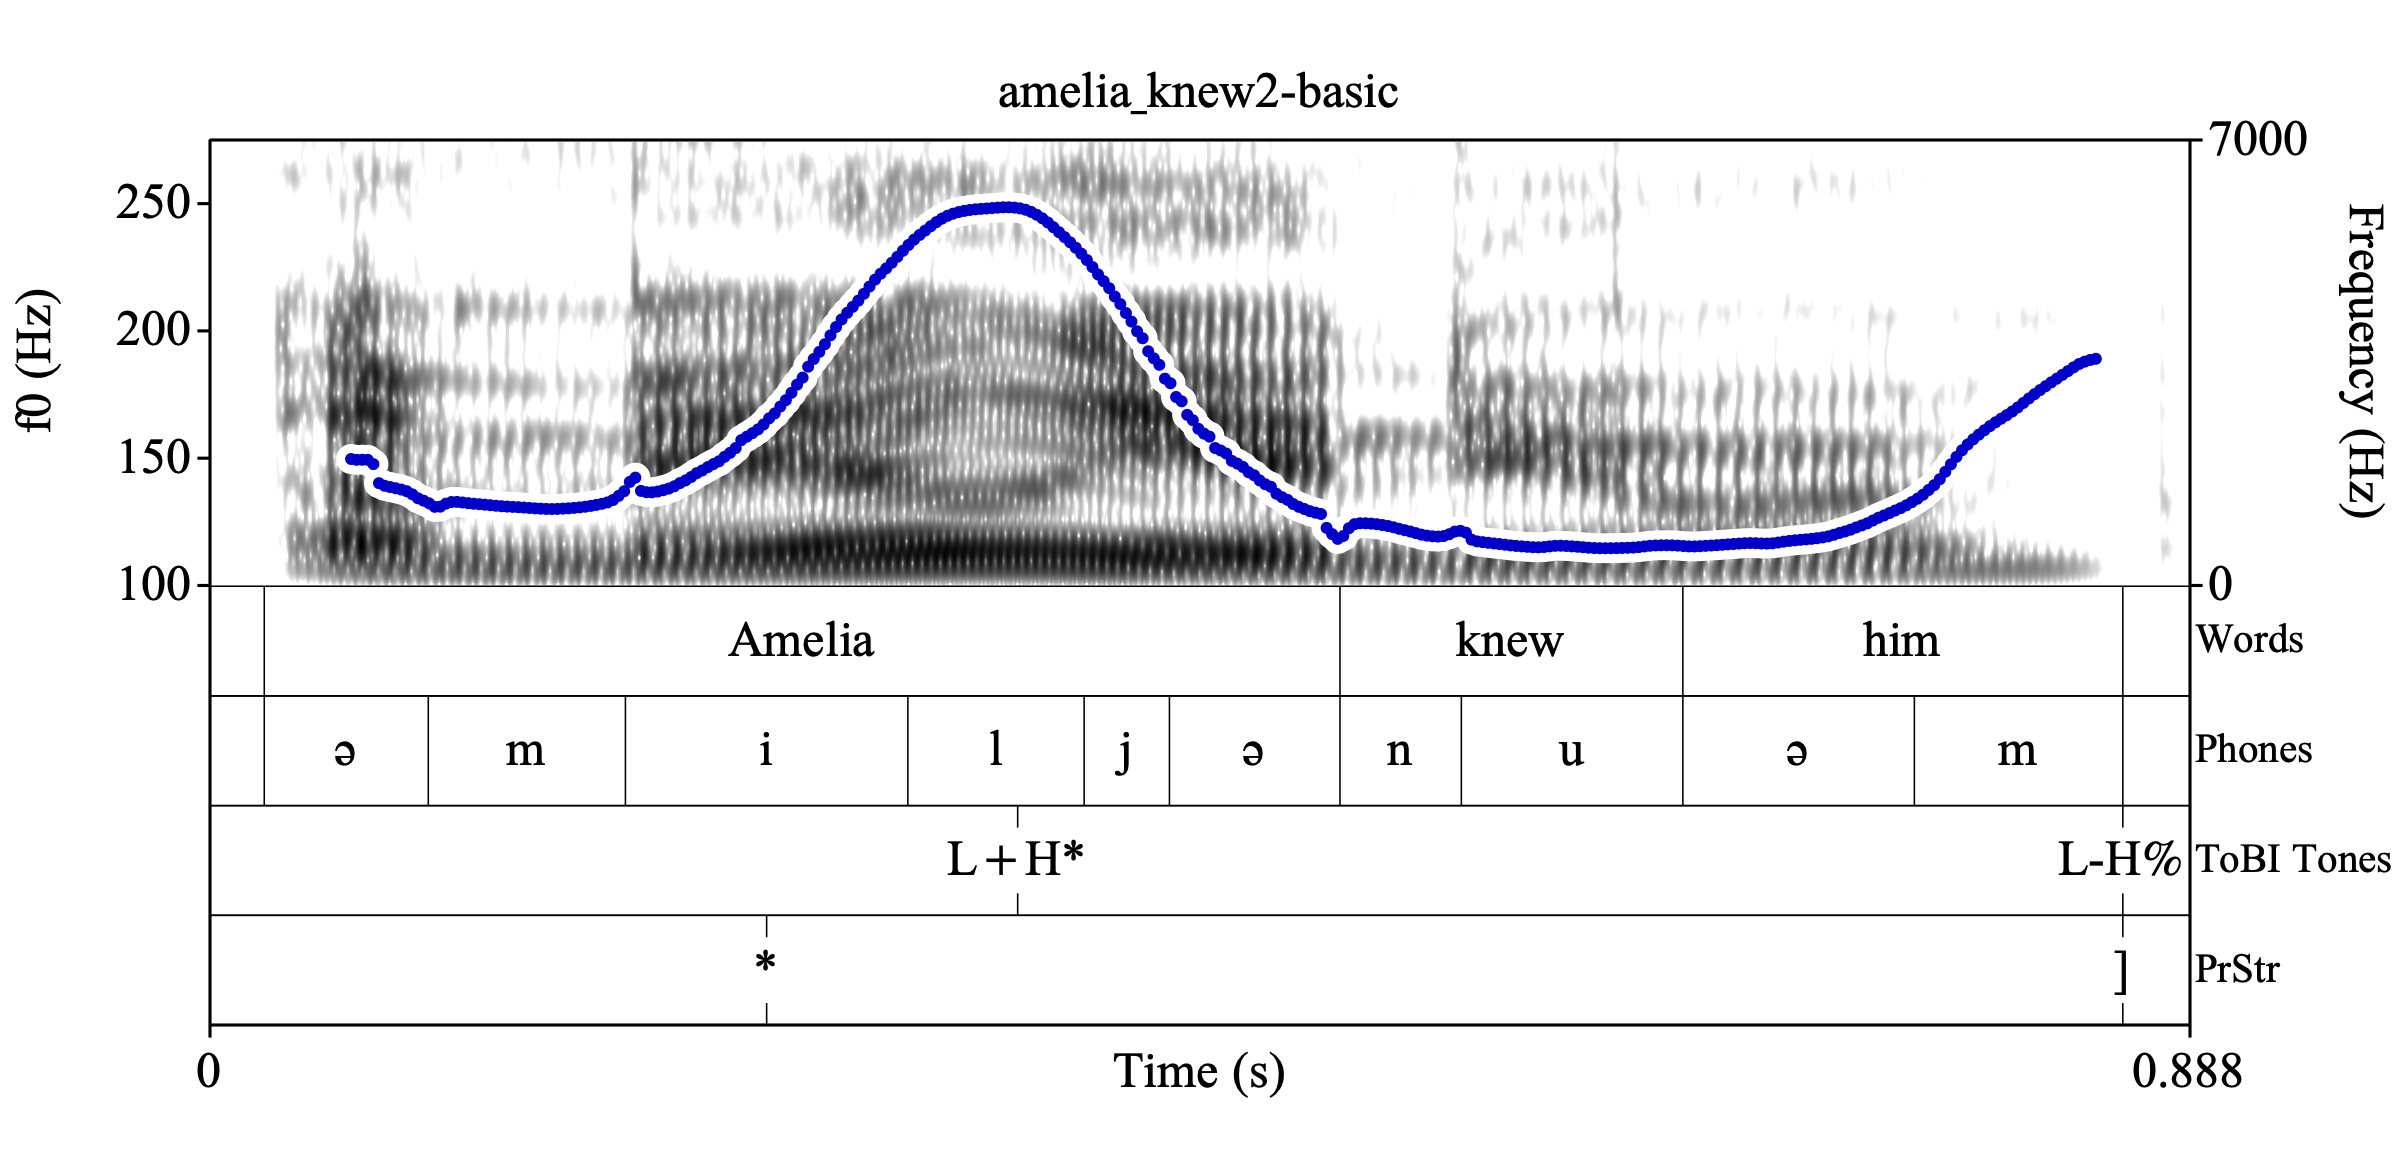
\includegraphics[width=.875\linewidth]{PrStr-amelia_knew2-basic.png}
%
\caption{\texttt{amelia-knew2}, with the PrStr tier annotated.%
\label{fig:amelia-knew2 PrStr}%
\index{Annotated example, PrStr tier (basic)!amelia-knew2}%
}
\end{figure}

\paragraph{Basic PrStr Examples  3 and 4: label locations}

Although changes in f0 are often very visually salient cues to prosodic structure, particularly prominences, PoLaR PrStr labels are situated with respect to the word string. Here the \textlabel{*} label is placed in the center of the transcribed [ɪ] vowel rather than at the f0 peak. The \textlabel{]} label is at the end of the final word in the phrase. 


\begin{figure}[H]
\centering
%
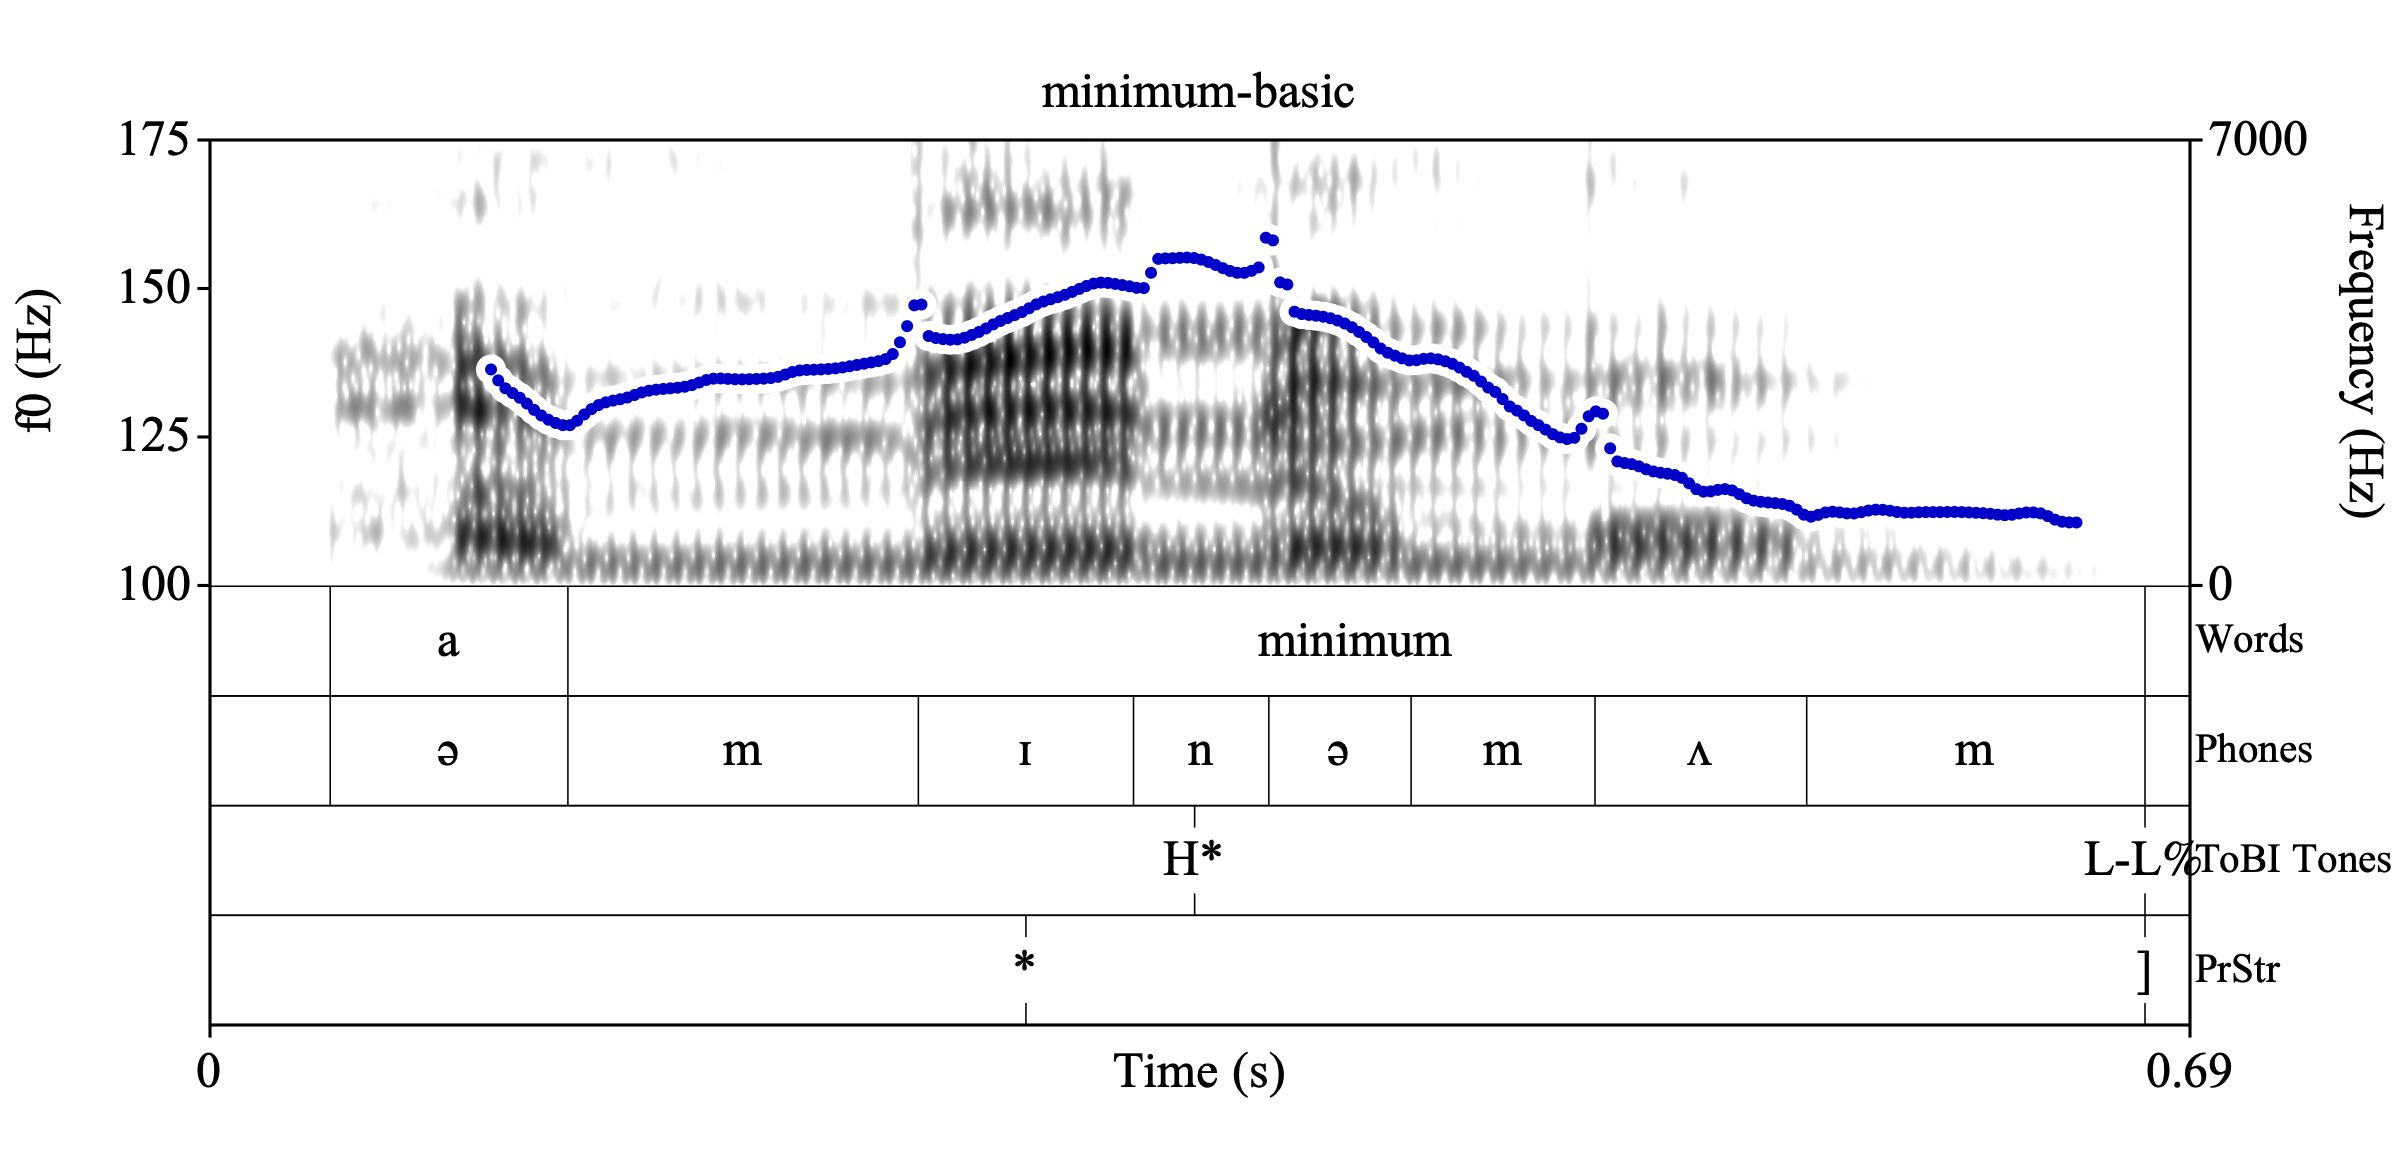
\includegraphics[width=.875\linewidth]{PrStr-minimum-basic.png}
%
\caption{\texttt{minimum}, with the PrStr tier annotated.%
\label{fig:minimum PrStr}%
\index{Annotated example, PrStr tier (basic)!minimum}%
}
\end{figure}

Similarly, the \textlabel{*} label is placed in the middle of the transcribed [i] rather than in the high f0 that cues the prominence. 

\begin{figure}[H]
\centering
%
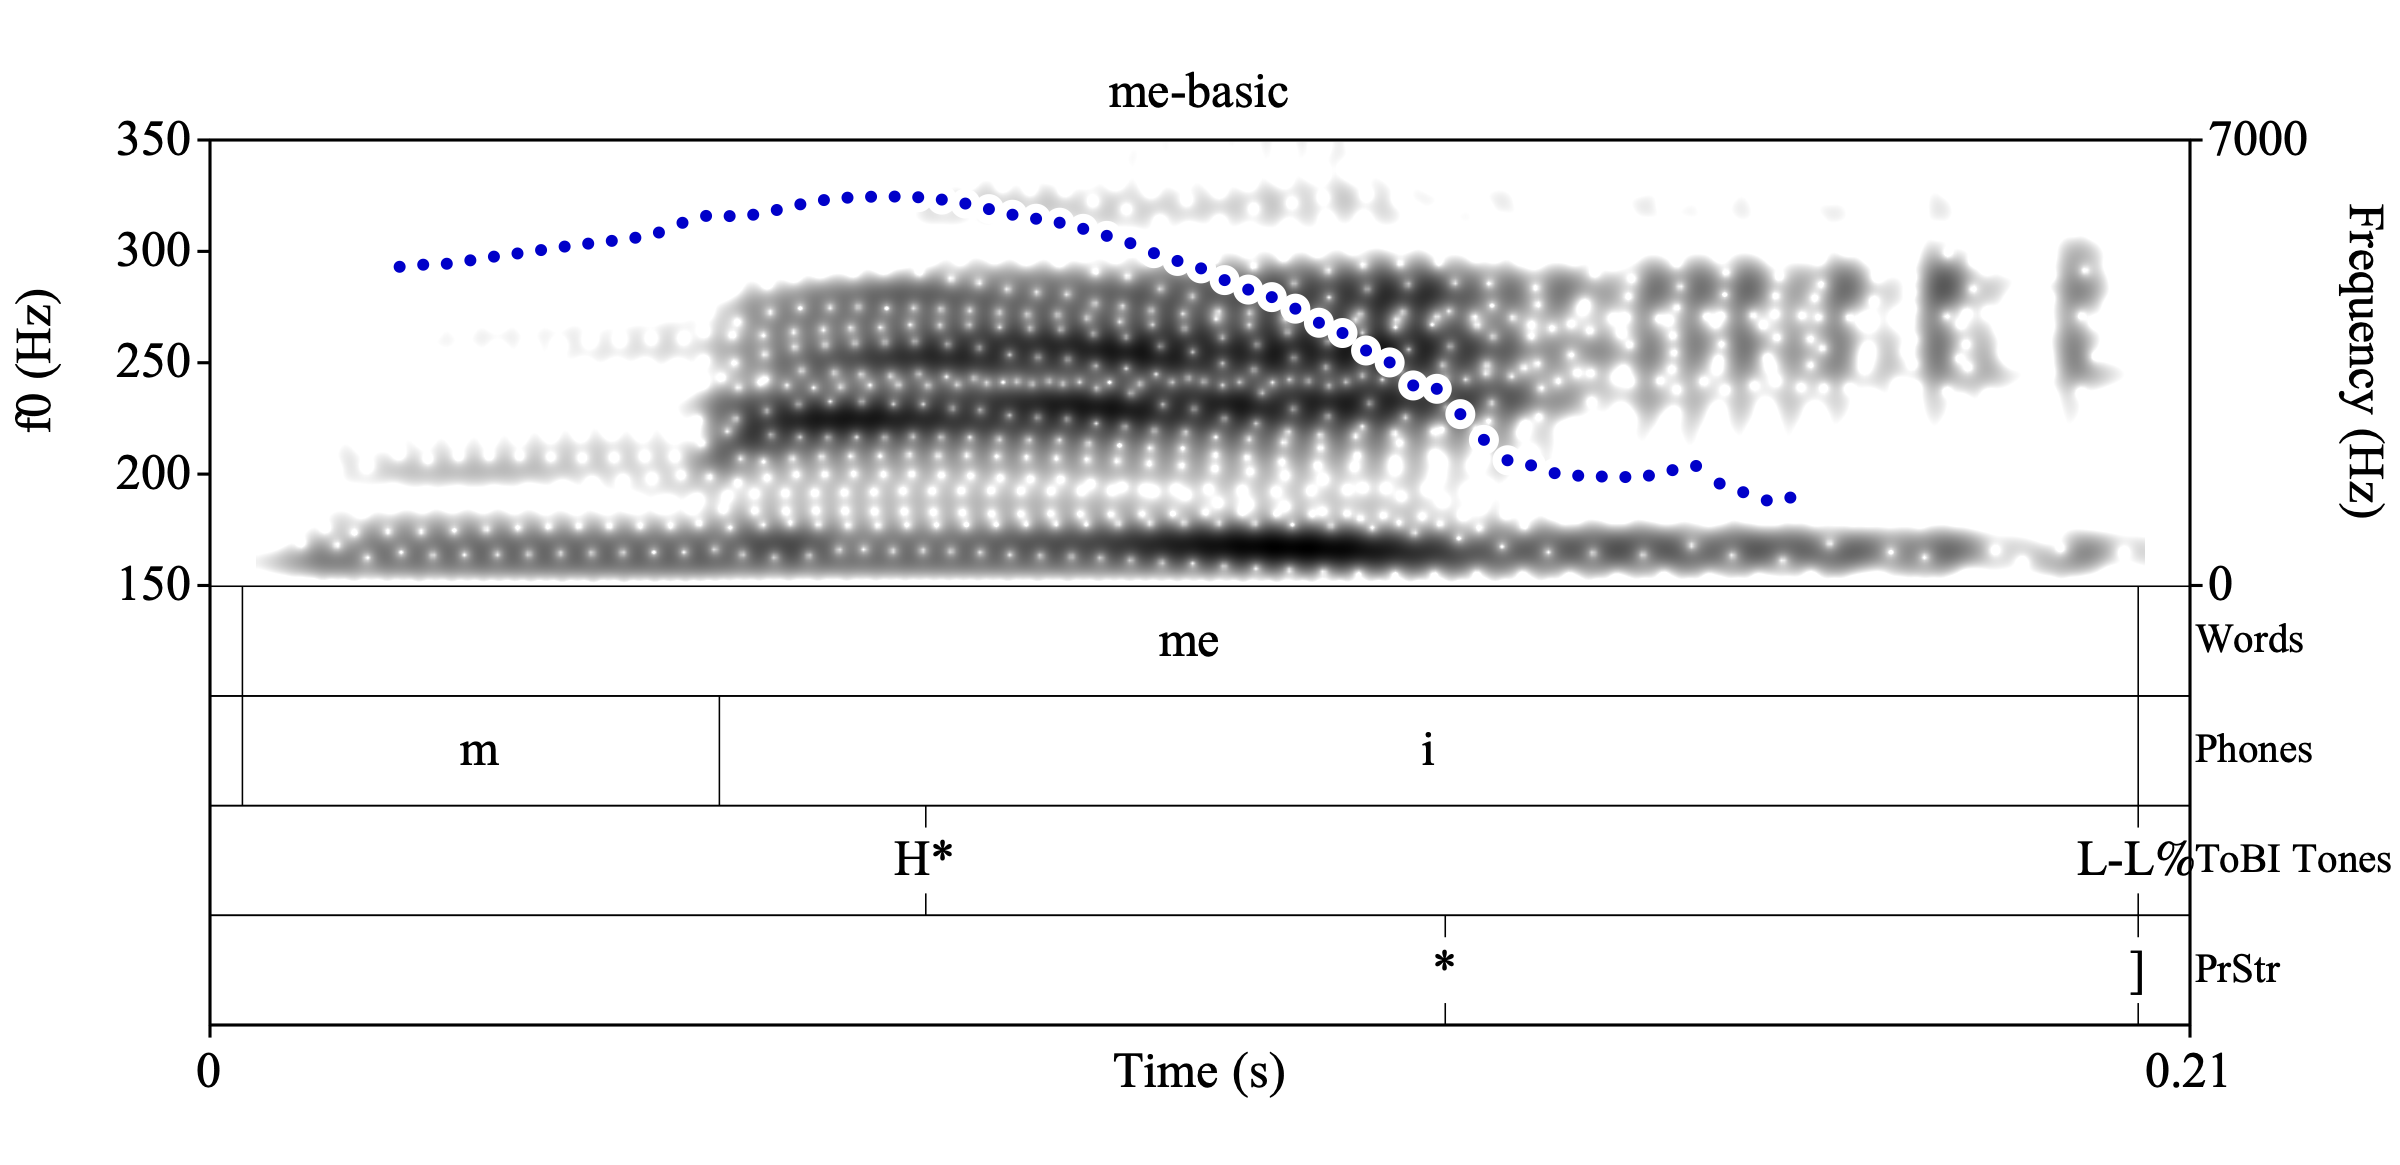
\includegraphics[width=.875\linewidth]{PrStr-me-basic.png}
%
\caption{\texttt{me}, with the PrStr tier annotated.%
\label{fig:me PrStr}%
\index{Annotated example, PrStr tier (basic)!me}%
}
\end{figure}

\paragraph{Basic PrStr Examples 5, 6, 7: multiple phrases and prominences in the same utterance}

Even short utterances can have more than one phrase. In general every phrase will have one or more prominences.  Labelers should use their intuitions as well as visual cues in the speech display to determine which words bear prominence or are in the same group.

\begin{figure}[H]
\centering
%
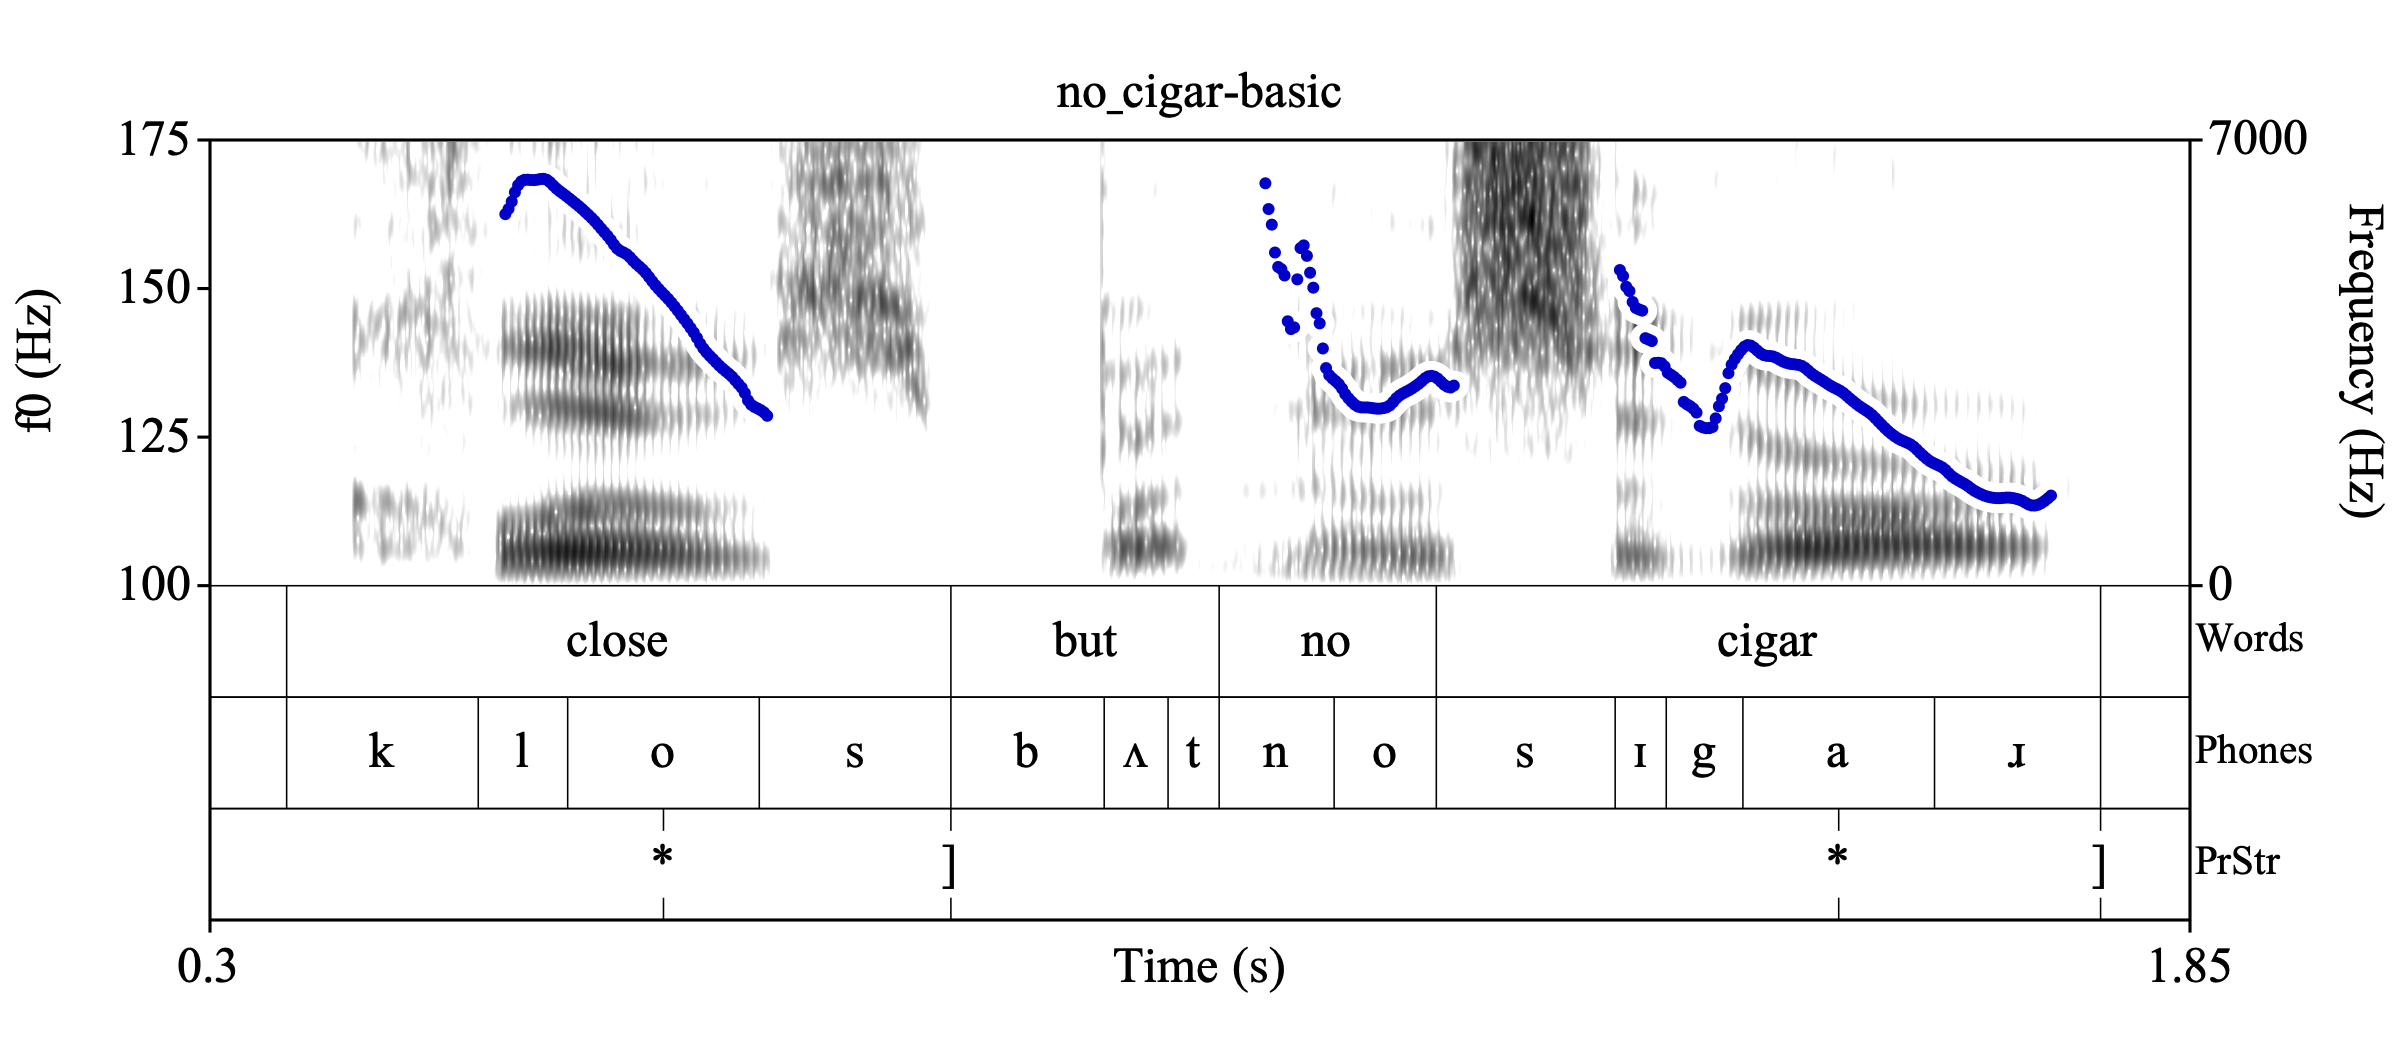
\includegraphics[width=.875\linewidth]{PrStr-no_cigar-basic.png}
%
\caption{\texttt{no\_cigar}, with the PrStr tier annotated.%
\label{fig:no_cigar PrStr}%
\index{Annotated example, PrStr tier (basic)!no\_cigar}%
}
\end{figure}

\begin{figure}[H]
\centering
%
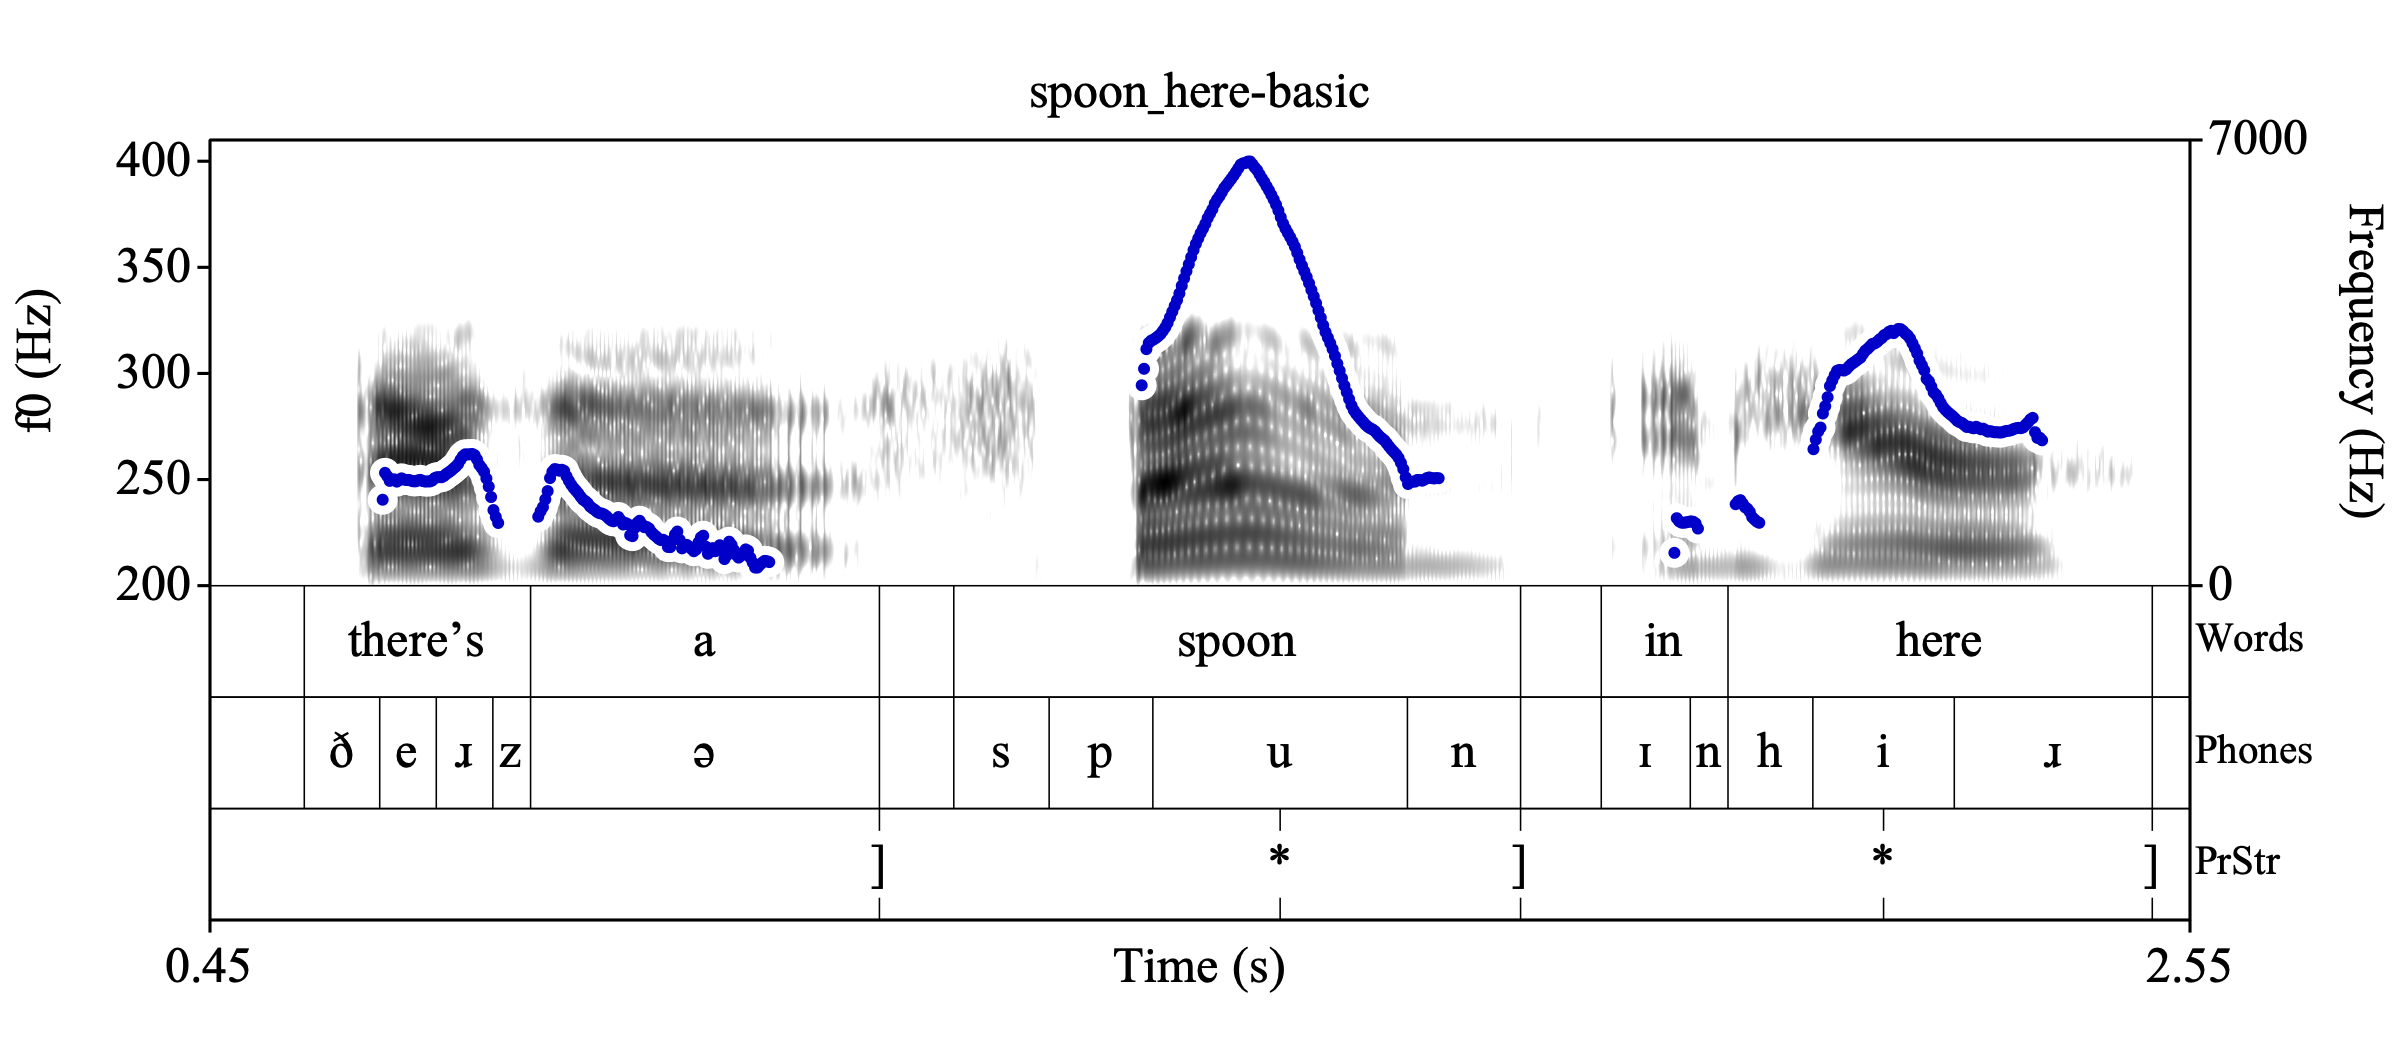
\includegraphics[width=.875\linewidth]{PrStr-spoon_here-basic.png}
%
\caption{\texttt{spoon\_here}, with the PrStr tier annotated.%
\label{fig:spoon_here PrStr}%
\index{Annotated example, PrStr tier (basic)!spoon\_here}%
}
\end{figure}

\begin{figure}[H]
\centering
%
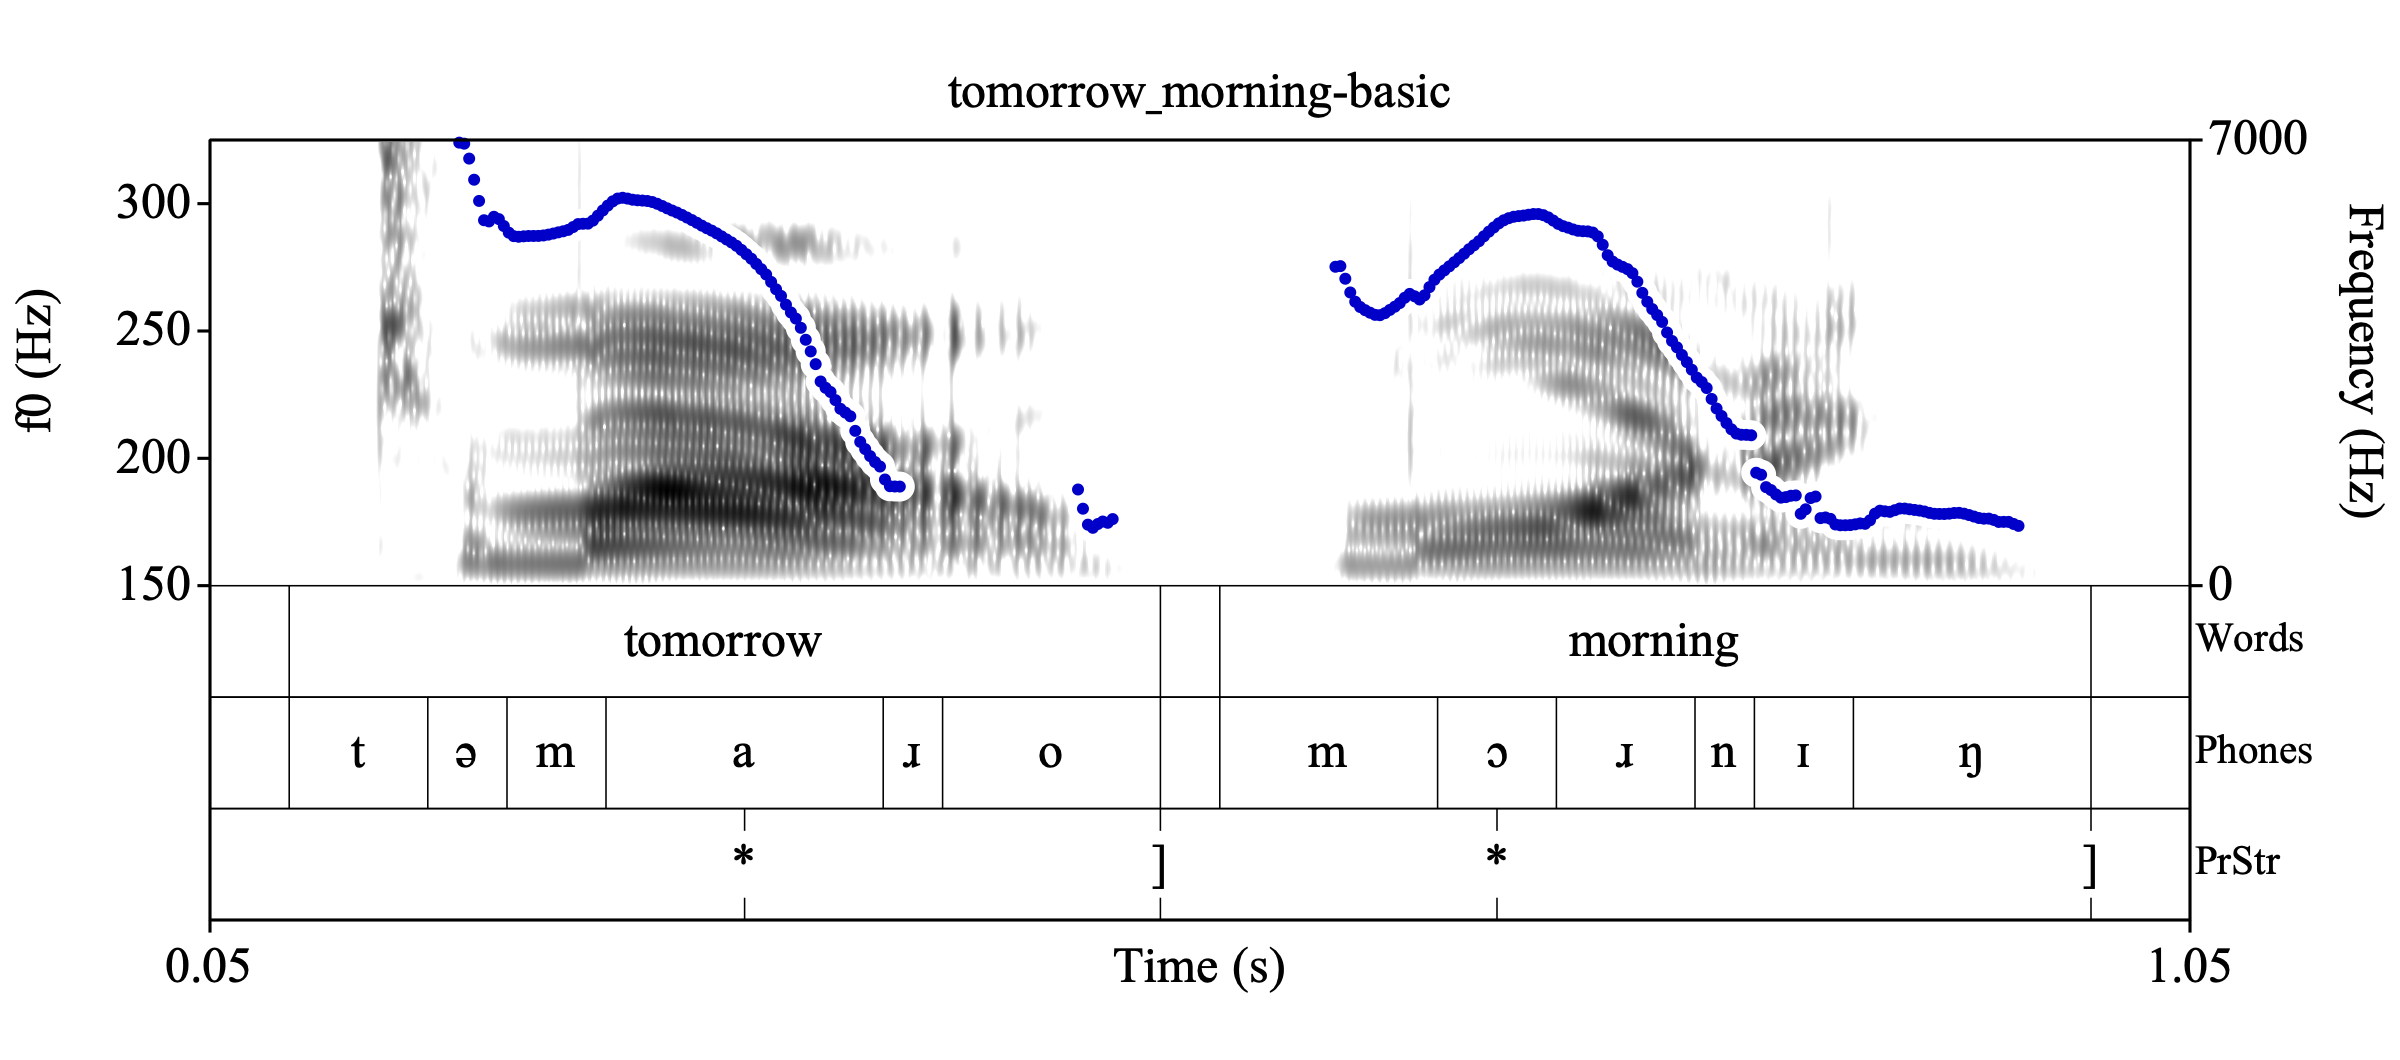
\includegraphics[width=.875\linewidth]{PrStr-tomorrow_morning-basic.png}
%
\caption{\texttt{tomorrow\_morning}, with the PrStr tier annotated.%
\label{fig:tomorrow_morning PrStr}%
\index{Annotated example, PrStr tier (basic)!tomorrow\_morning}%
}
\end{figure}

\paragraph{Basic PrStr Examples 8 and 9: F0 failure to fall}
As a cautionary note to labelers not to rely solely on the visual f0 displays (even when they are relatively accurate): not all prominences can be identified with notable rise-fall peaks. The following examples show that prominences on a series of words might be cued with a steady high f0 that doesn’t fall in between. 

\begin{figure}[H]
\centering
%
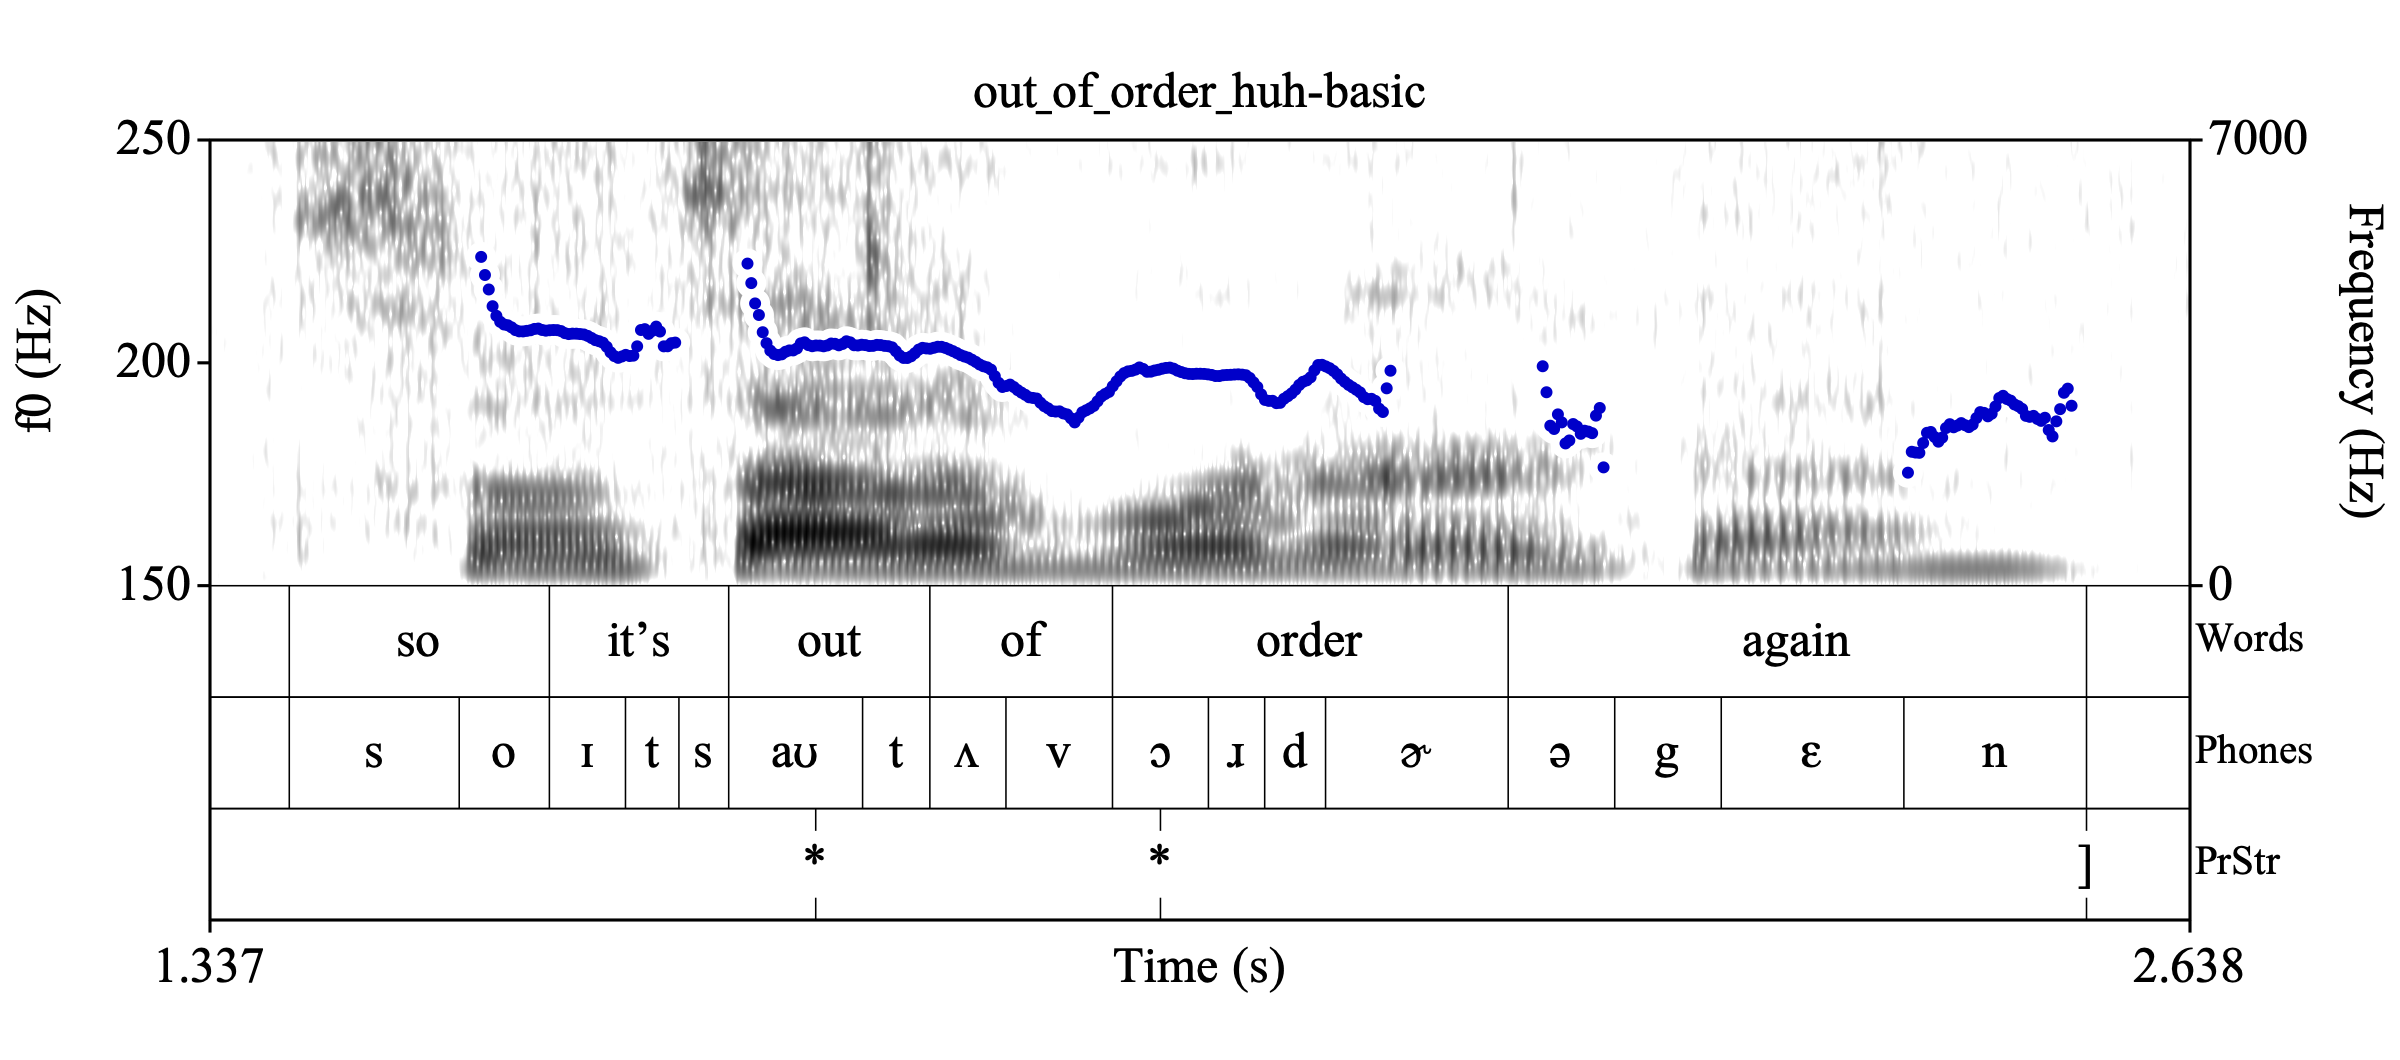
\includegraphics[width=.875\linewidth]{PrStr-out_of_order_huh-basic.png}
%
\caption{\texttt{out\_of\_order\_huh}, with the PrStr tier annotated.%
\label{fig:out_of_order_huh PrStr}%
\index{Annotated example, PrStr tier (basic)!out\_of\_order\_huh}%
}
\end{figure}

\begin{figure}[H]
\centering
%
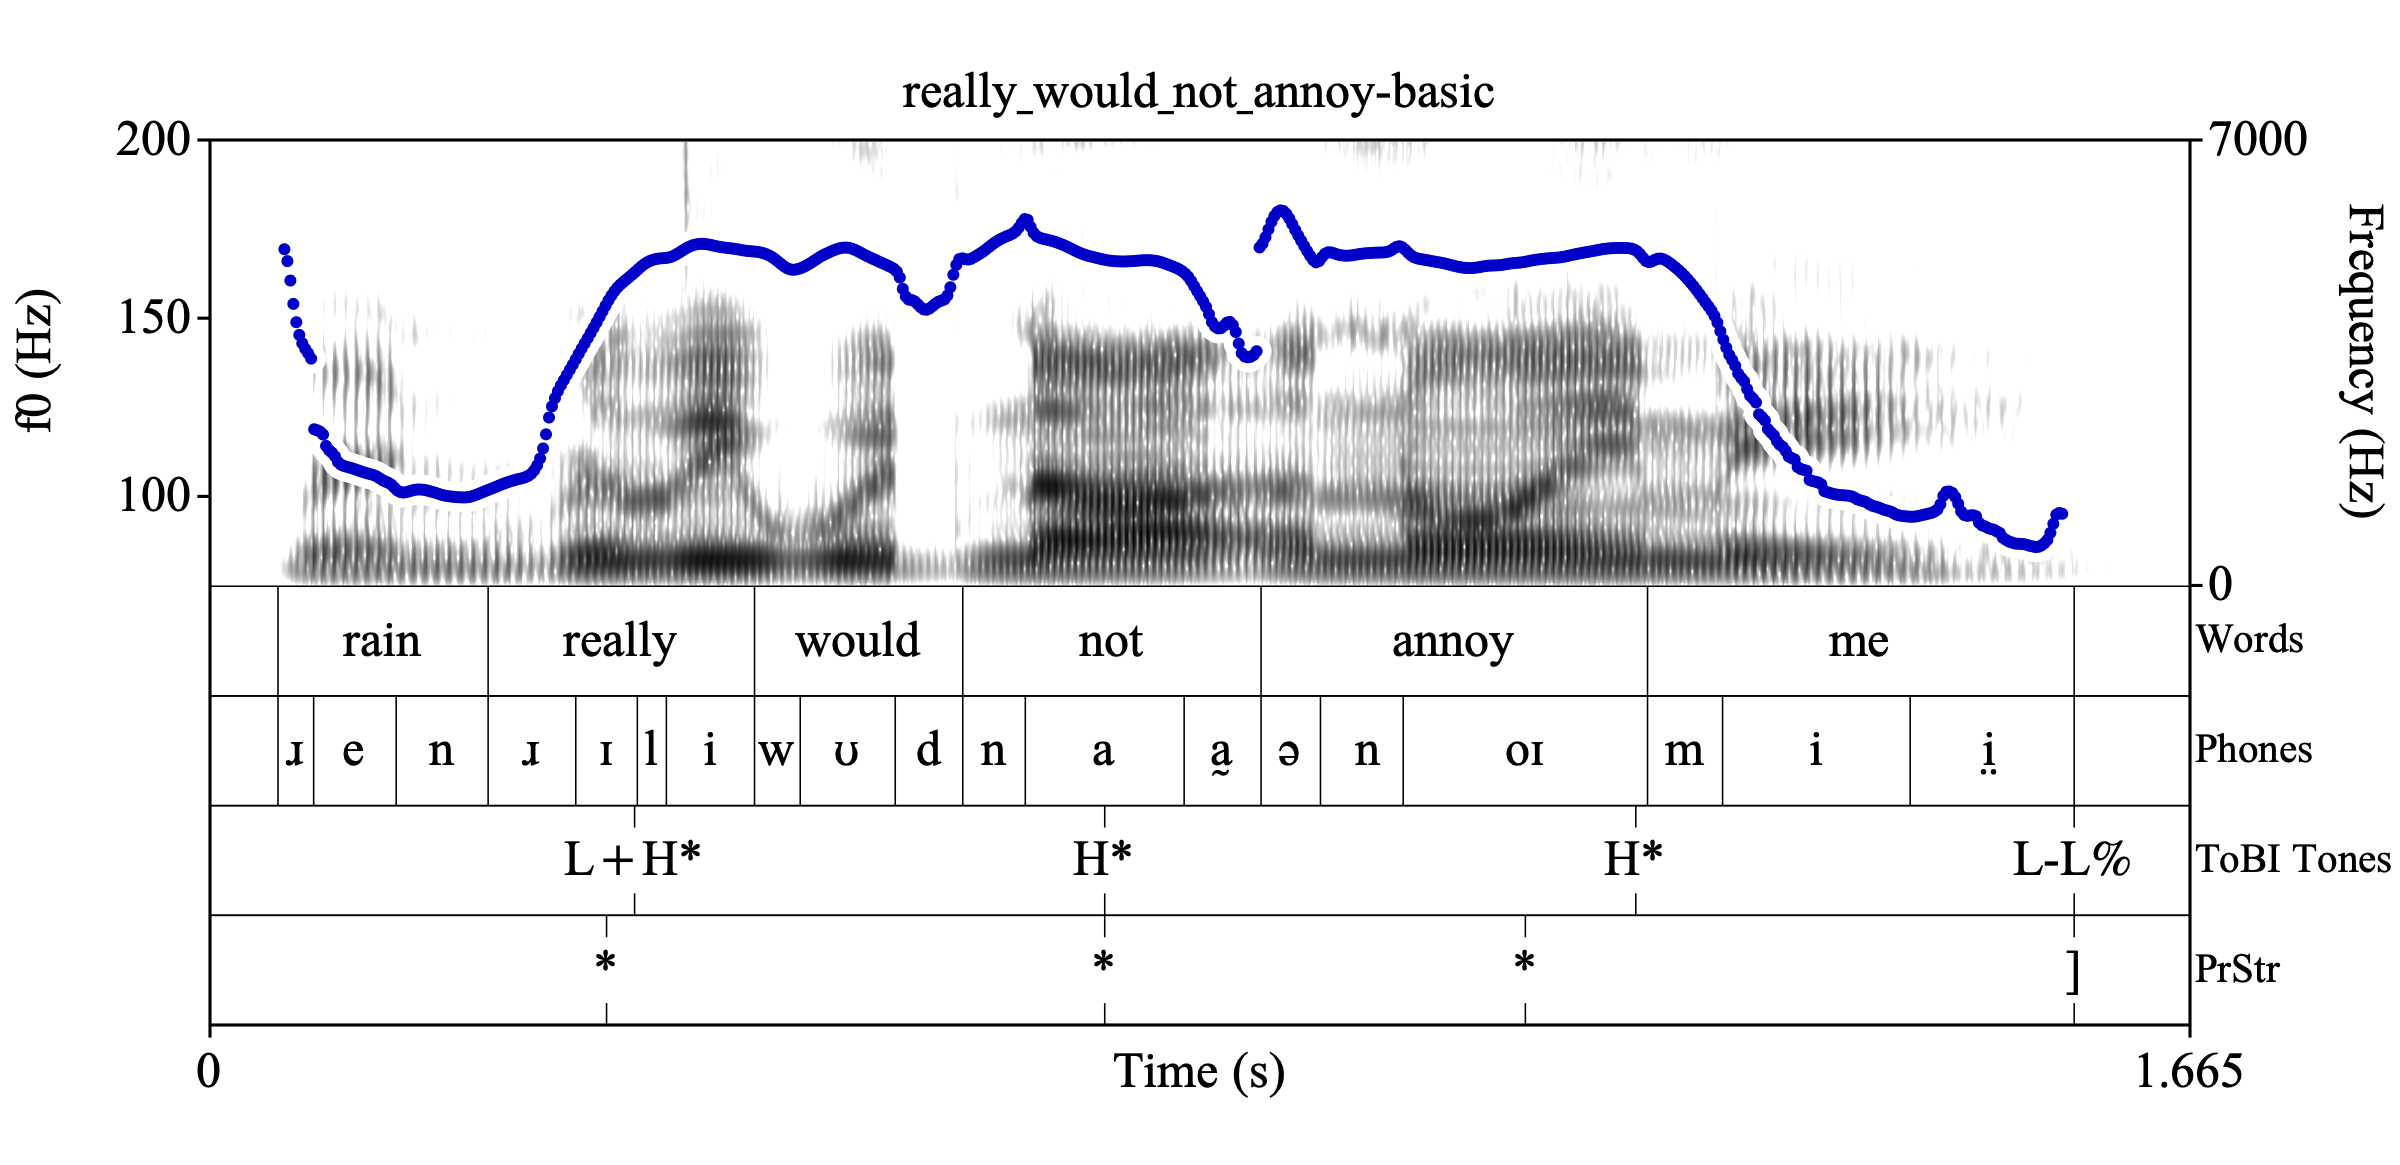
\includegraphics[width=.875\linewidth]{PrStr-really_would_not_annoy-basic.png}
%
\caption{\texttt{really\_would\_not\_annoy}, with the PrStr tier annotated.%
\label{fig:really_would_not_annoy PrStr}%
\index{Annotated example, PrStr tier (basic)!really\_would\_not\_annoy}%
}
\end{figure}


\subsubsection{PrStr labels summary}\label{sec:prstr-labels-summary}

The four PrStr Basic labels are named in Table \ref{PrStr basic labels}.

\begin{longtable}{clp{.525\linewidth}} \toprule \textbf{Label} & \textbf{Phonological Object} & \textbf{Label is time-aligned with \_\_\_\_\_}\tabularnewline
\midrule \endhead
\textlabel{*} & Prominence & A syllable that has intonational prominence \tabularnewline
\textlabel{?*} & Possible Prominence & A syllable that might have intonational prominence \tabularnewline
\textlabel{]} & Phrase’s Right Edge & The right edge of the final word of a phrase \tabularnewline
\textlabel{?]} & Possible Phrase’s Right Edge & What might be the right edge of the final word of a phrase \tabularnewline
\bottomrule 
\caption{The Basic labels for the Prosodic Structure tier (for English).%
\label{PrStr basic labels}%
}
\end{longtable}

\subsection{Points Tier}\label{sec:points}

With the Points Tier, we will focus on the changes in pitch, as observed through changes in fundamental frequency (f0). When discussing the pitch changes in an intonational contour, some approaches aim to define them as a sequence of phonological objects (e.g., a low pitch accent followed by a steady rise to a high boundary tone). However, such phonological objects are not directly observed in the acoustics, but rather are signalled with a variety of cues (e.g., pitch, duration, intensity, voice quality, etc.) – the primary purpose of the PoLaR Points tier is to identify the fundamental shape of the intonational contour.

\begin{infobox}[frametitle=\textbf{A NOTE ON TERMINOLOGY}]
Recall that f0 and pitch are different: f0 values can be measured directly from the speech signal, while pitch values are psycho-perceptual. Parallel to this, f0 contours track changes in f0 values, while intonational contours refer to abstract changes in pitch. Return to section \ref{sec:terminology} in Chapter \ref{ch:background} for more detailed discussion.\label{terminology f0 pitch}
\end{infobox}

PoLaR allows two levels of annotation detail on the Points Tier: the default (‘\textlabel{0}’) label is described in this chapter. (Advanced labels for associating the pitch turning points on the Points tier with the prosodic events on the PrStr tier, are described in Chapter \ref{ch:advanced}.)

Regardless of whether a labeller is using Basic or Advanced labels, the Points Tier is used to capture those significant turning points in a point-in-time tier. The goal (guidance below) is to annotate only and all of the f0 locations that are perceptually salient. (We will describe some f0 movements that are \emph{not} perceptually salient, later in this section.) Consider the f0 contour in the following example:

\begin{figure}[H]
\centering
%
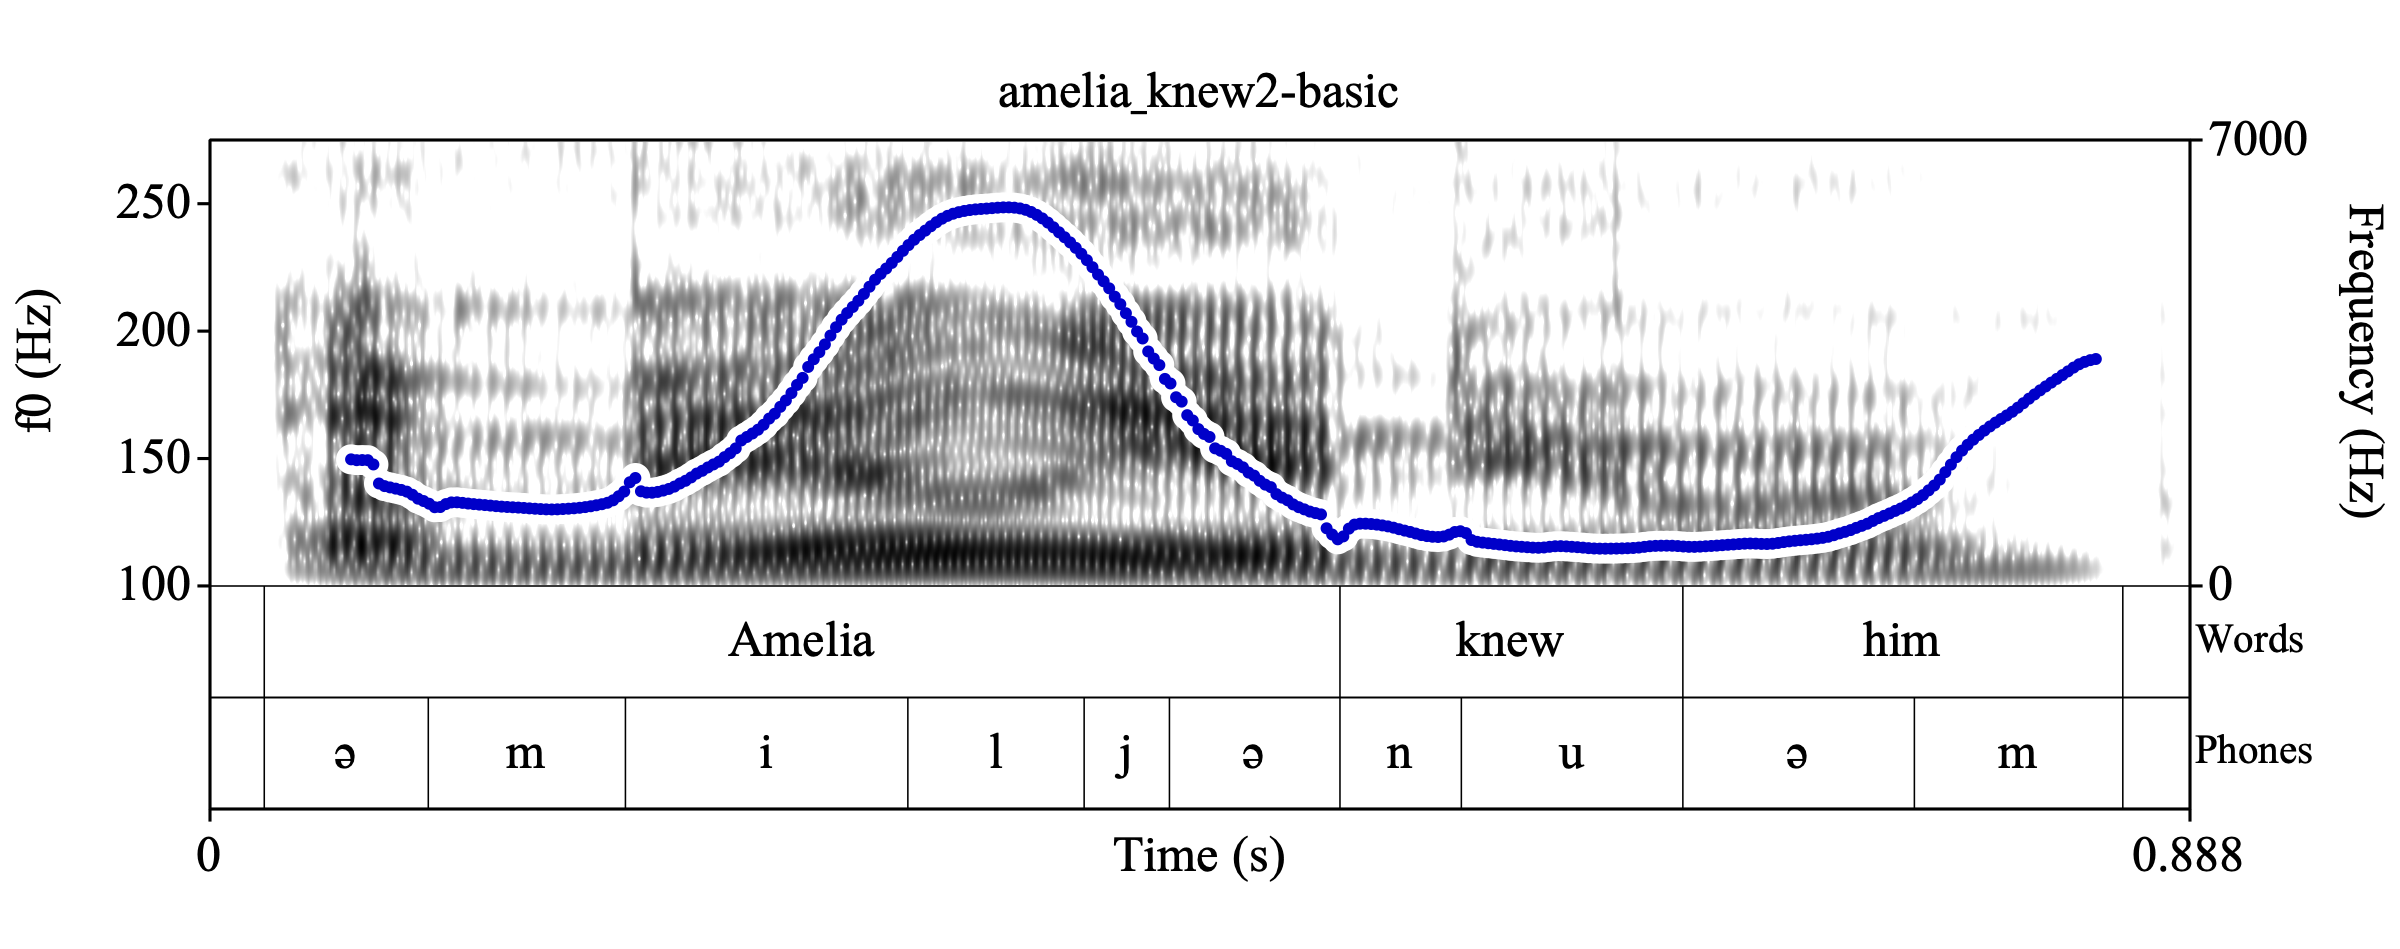
\includegraphics[width=.875\linewidth]{Points-amelia_knew2-f0.png}
%
\caption{The f0 contour for \texttt{amelia\_knew2}.%
\label{fig:amelia_knew2 f0 contour}%
%\index{Annotated example, Points tier (basic)!XXXX}%
}
\end{figure}

One can think of the pitch in the intonational contour as closely related to particular “f0 turning points”. These inflection points in the f0 curve are locations in time where the rate of rise\slash fall changes (that is, the change in the second derivative of the (usually smoothed) f0). The f0 turning points for this last example might be found at the dots below:

\begin{figure}[H]
\centering
%
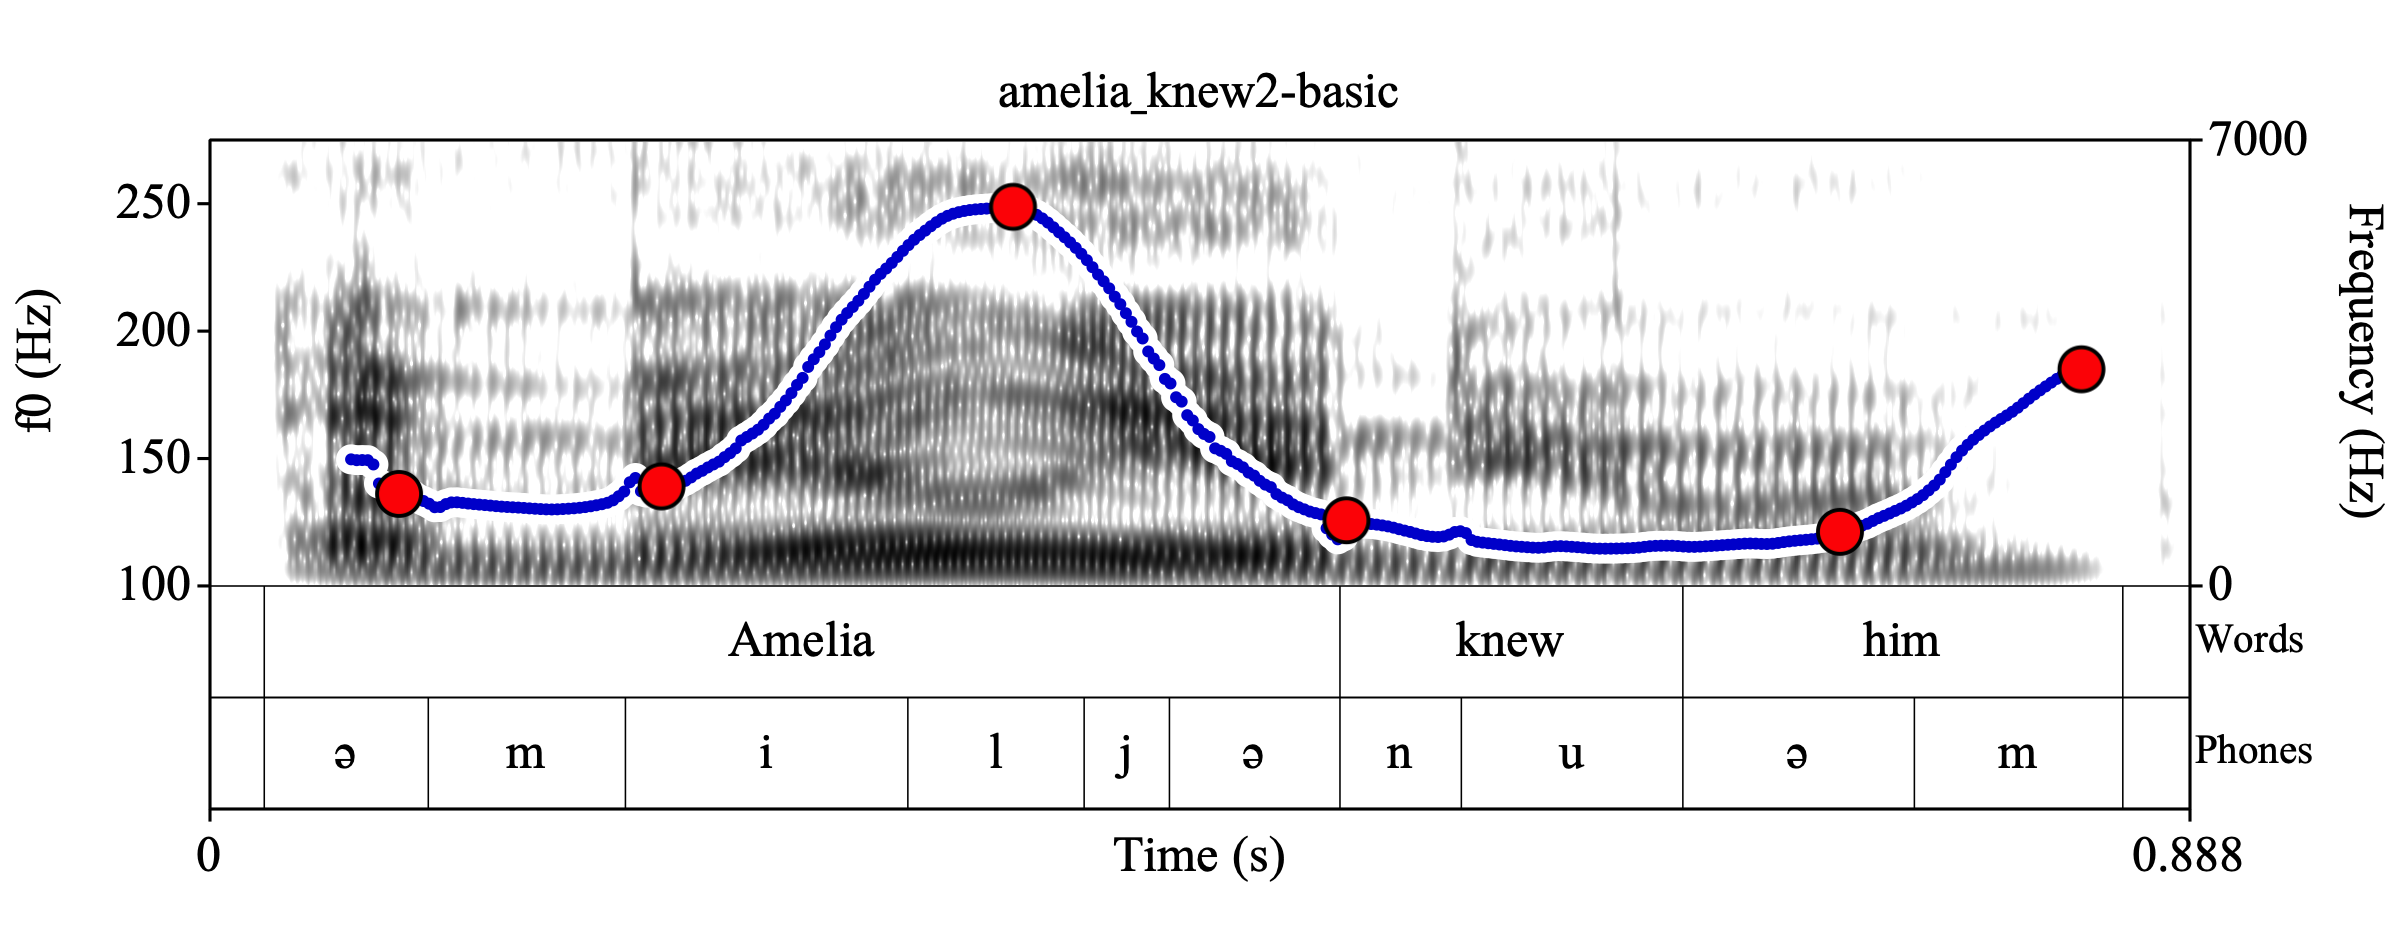
\includegraphics[width=.875\linewidth]{Points-amelia_knew2-f0-dots.png}
%
\caption{The f0 contour for \texttt{amelia\_knew2}, visually annotated for f0 turning points.%
\label{fig:amelia_knew2 f0 contour turning points}%
%\index{Annotated example, Points tier (basic)!XXXX}%
}
\end{figure}

\begin{infobox}[frametitle=\textbf{PRACTICAL SUGGESTIONS}]
 Care must be taken to control pitch settings so that the labelling field is not too wide (“zoomed out”) and that the minimum\slash maximum range choices result in a contour as dynamic and smooth as possible. (See also the discussion of software settings in section \ref{sec:software-effects}.) For discussion of which turning points require labelling, and how to use straight-line-segment resynthesis to aid in making these decisions, see section \ref{sec:points-tier-transcription}.
\end{infobox}

The resulting labels are aligned with these significant turning points on the Points Tier, using the default Basic label ‘\textlabel{0}’ :

\begin{figure}[H]
\centering
%
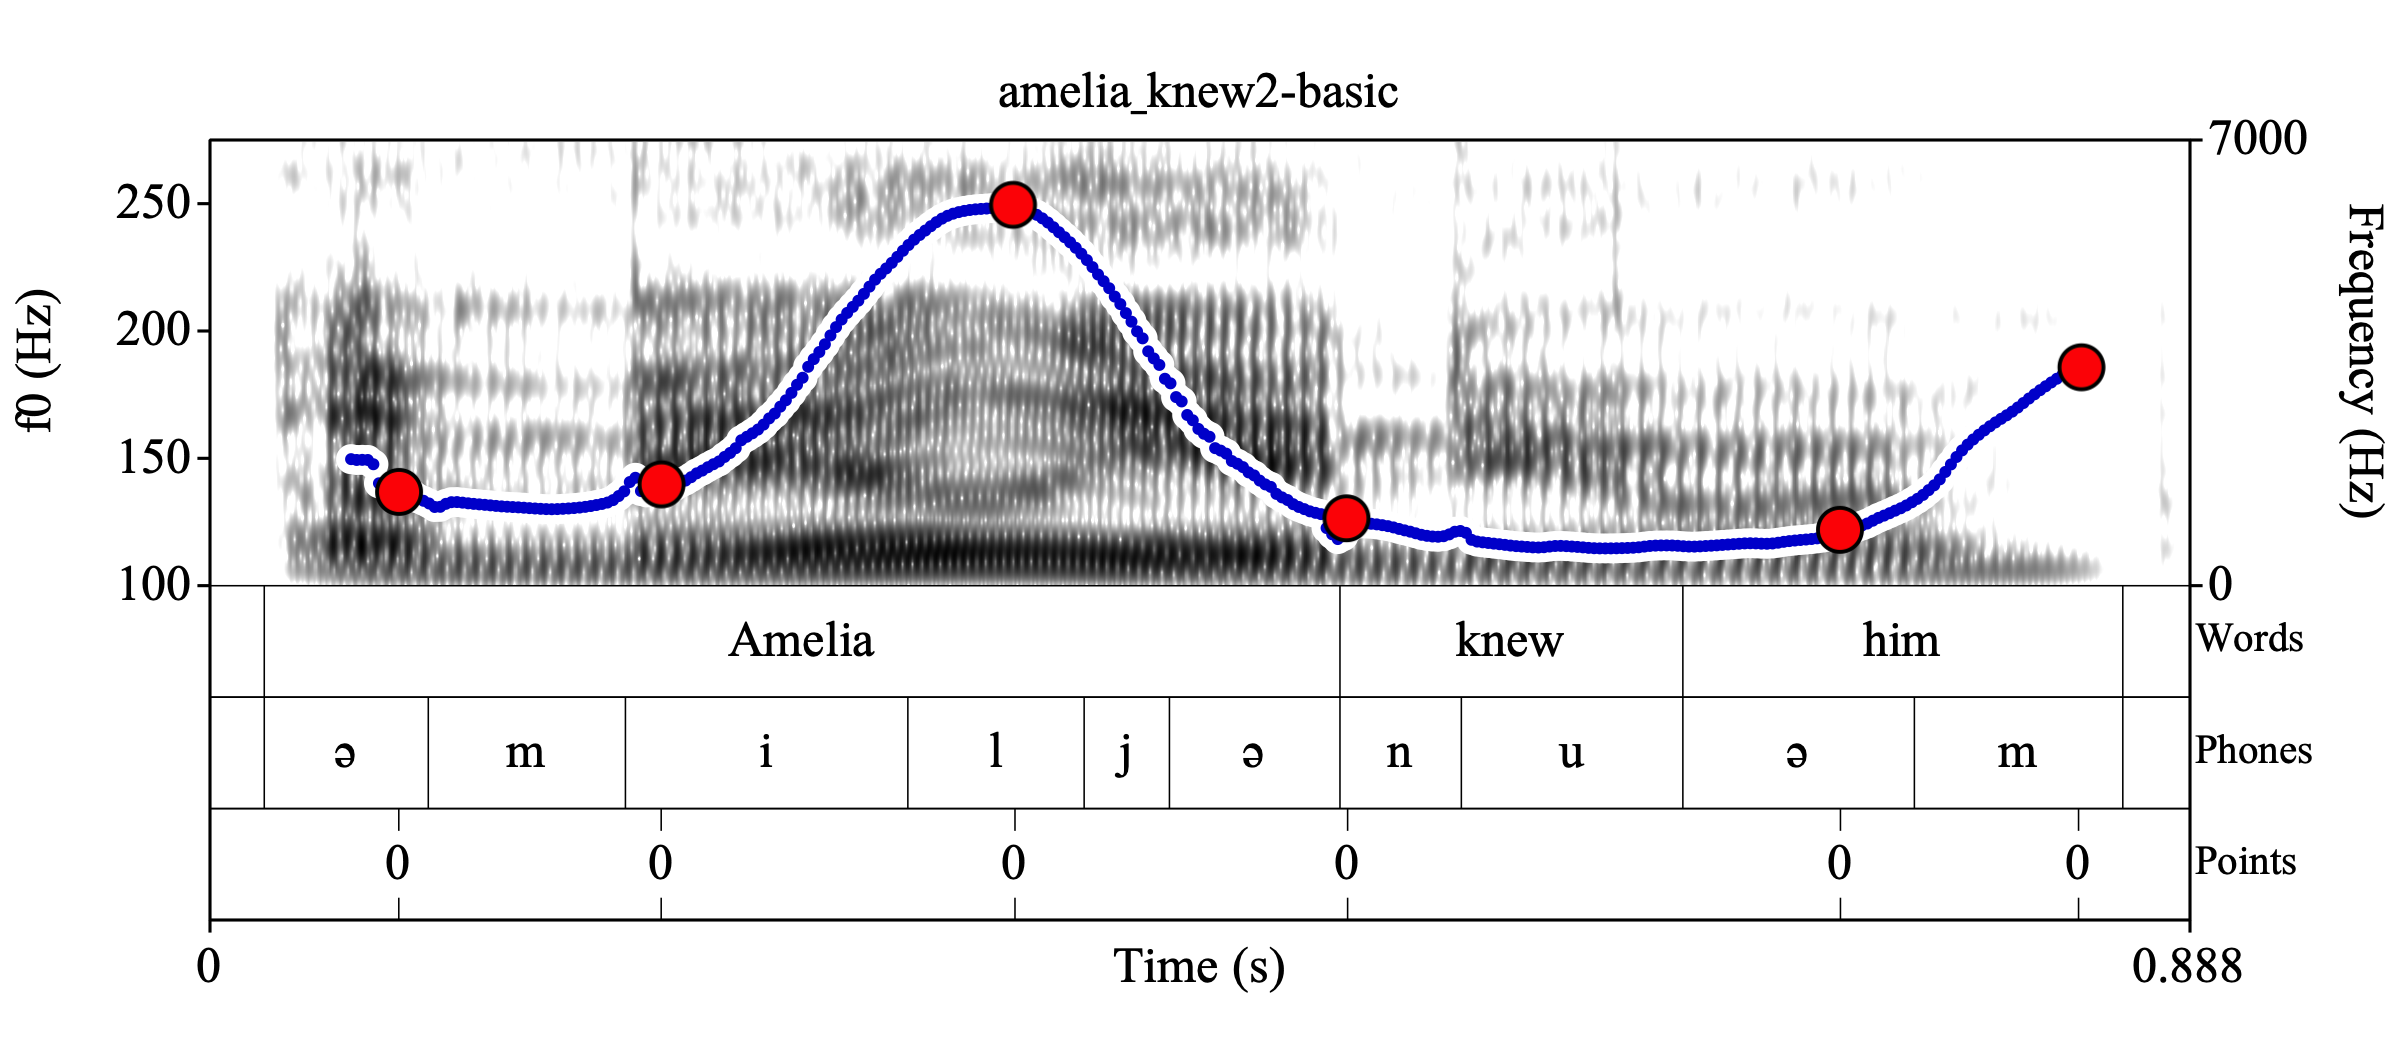
\includegraphics[width=.875\linewidth]{Points-amelia_knew2-basic-dots.png}
%
\caption{The f0 contour for \texttt{amelia\_knew2}, with the Points tier annotated with Basic ‘\textlabel{0}’ labels.%
\label{fig:amelia_knew2 f0 contour turning points 0 labels}%
\index{Annotated example, Points tier (basic)!amelia\_knew2}%
}
\end{figure}

It is important to note that PoLaR allows an annotator to label \uline{\textit{\textbf{any}} (salient) f0 turning point. This contrasts with other,} more phonologically oriented annotation systems (e.g., ToBI, IViE), in which an annotator can only capture a pitch movement by using a label that also indicates an analysis related to the presence of a phonological object.\footnote{As a concrete example, an annotator using such a system can only capture a pitch movement to high pitch if it corresponds to a pitch accent (\textlabel{H*}) or boundary tone (\textlabel{H-} or \textlabel{H\%}). This may be particularly important for the exploration of unfamiliar languages or understudied varieties.} As such, PoLaR intends to capture all significant pitch movements – even those which may not cue a phonological object (at least not in current intonational grammars).\footnote{That is, there may be (potentially systematic) pitch movements that are not predicted by prominence\slash phrasing as we understand them and their relationship to intonation, but which manifest as perceptible movements in the f0 tracking.} We describe more in the next section about what guides whether or not to label a given pitch movement.

\subsubsection{Points Tier Transcription}\label{sec:points-tier-transcription}

The disentangling of turning points from the events labelled on the PrStr tier raises an important question: \textbf{What does and does not get labelled as an f0 turning point?} The answer to this is primarily determined by the main goal of PoLaR’s Points labelling: to capture enough information to identify any\slash all \textbf{systematic patterns} in the f0 curve, without simply replicating the entire curve, point by point, on the Points tier.

In this monograph, we are not aiming to provide an exhaustive account of what should or should not be annotated; instead, we aim to provide \uline{some basic guidelines}. First, is the guideline that the annotator \uline{should not} label f0 movements that are due to the influence of segments\footnote{We do not rule out the possibility of using PoLaR to annotate segmental effects with the goal of learning more about which microprosodic effects are linked to which segments. Indeed, PoLaR would make a good candidate for annotating such changes. However, for general uses of PoLaR, labellers are advised to ignore microprosody. See section \ref{sec:intonational-contours-and-software-based-pitch-tracks} for more discussion.} (sometimes called “microprosody”, even though such f0 movements are not always small), environmental factors (e.g., background noise), or issues with recording-quality (e.g., electrical hums). At the same time, the annotator \uline{certainly should} label all peaks, plateaus, elbows, valleys, etc. that are intonationally salient and/or correspond to PrStr tier objects.

A second guideline to help determine which turning points are perceptually salient is to test the sequence of labelled points in a straight line approximation fidelity test (cf. straight line approximations as implemented by IPO, \citealt{t-hart-90}, and discussed in section \ref{sec:intonational-contours-and-software-based-pitch-tracks}). This test involves \uline{resynthesizing} the pitch of a recording as a sequence of line segments; this is described in the next section.

\subsubsection{Identifying Necessary Points Labels with Straight Line Approximations}\label{sec:identifying-necessary-points-labels-with-straight-line-approximations}

The concept of straight line approximations and a demonstration of how to use Praat to produce one will employ the example above (\texttt{amelia\_knew2}). In Figure \ref{fig:amelia_knew2 resynth}, the original pitch track is shown with a grey dotted line (note its curvature); however, if we use the same points as identified in Figure \ref{fig:amelia_knew2 f0 contour turning points 0 labels} to define the endpoints of line segments, we can get a pitch track as the one shown as the solid green line. Resynthesizing the pitch on the basis of this green line produces an utterance that is perceptually the same as the original. (Audio can be found as \texttt{amelia\_knew2-resynth} on \url{https://www.polarlabels.com}.)

\begin{figure}[H]
\centering
%
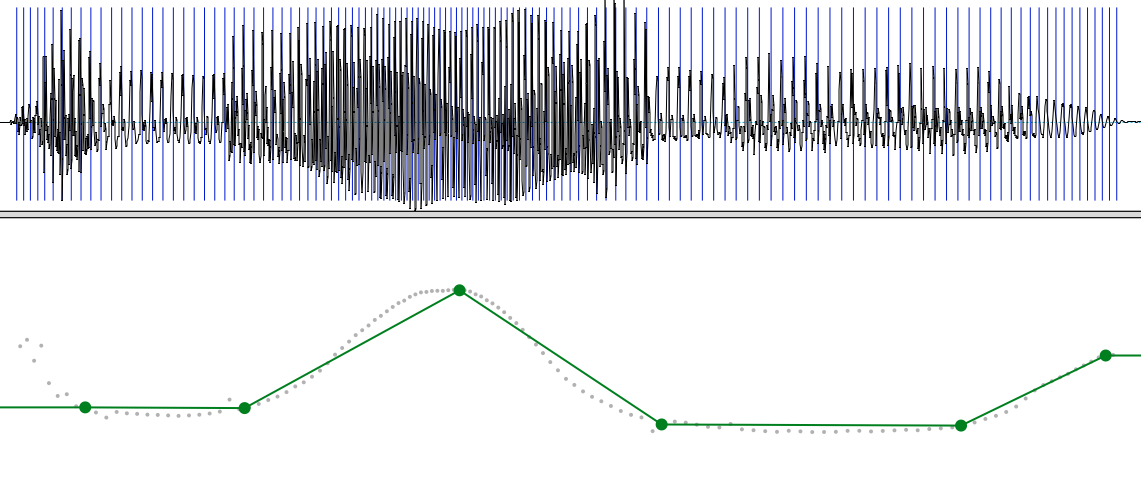
\includegraphics[width=.875\linewidth]{Points-amelia_knew2-resynth.png}
%
\caption{\texttt{amelia\_knew2}, with the resynthesized pitch in green, and the original pitch dotted gray.%
\label{fig:amelia_knew2 resynth}%
%\index{Annotated example, Points tier (basic)!XXXX}%
}
\end{figure}

The PoLaR plugin for Praat (found at the OSF repository linked from \href{https://www.polarlabels.com}{www.polarlabels.com}) automates the resynthesis – though only under the guidance of Points-tier labels provided by PoLaR annotators. (That is, the script is not fully automated, acting on its own; it relies on the human intuition of labellers.) With the plugin installed, users can click on the “Tier” menu and select “PoLaR: Resynthesize Straight Line Approximation”, and this will resynthesize the sound file, based on the pitch track and the timing of the Points tier labels.

\begin{figure}[H]
\centering
%
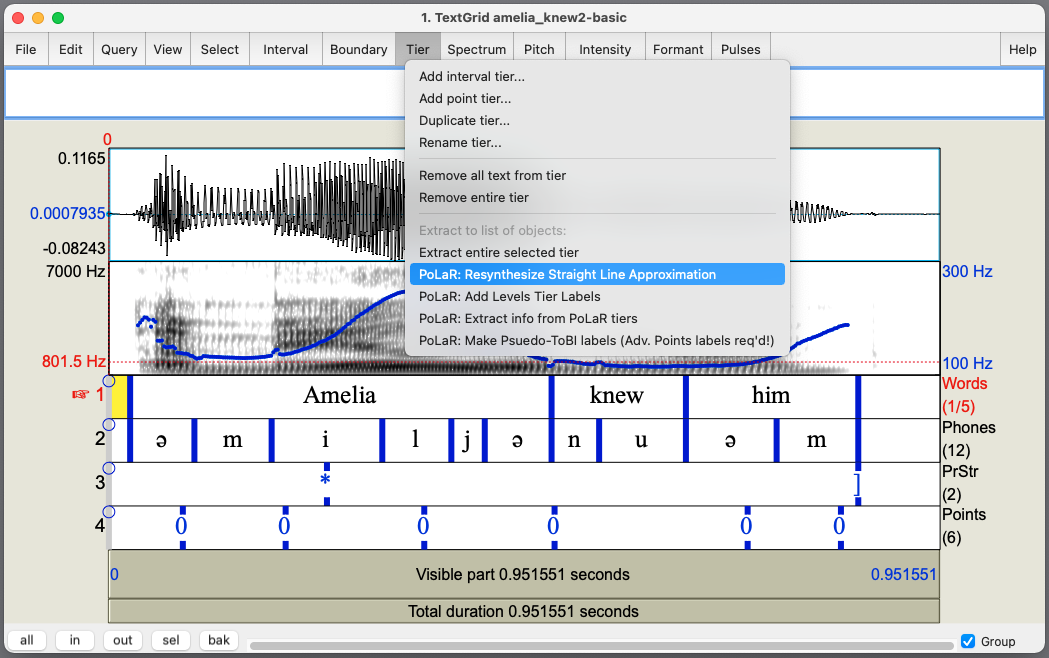
\includegraphics[width=.875\linewidth]{Points-amelia_knew2-before-SLA.png}
%
\caption{Running the Straight Line Approximation script, from the Praat menu in the Editor window.%
\label{fig:amelia_knew2 SLA menu}%
%\index{Annotated example, Points tier (basic)!XXXX}%
}
\end{figure}

This script can be especially useful as a way to test whether a given f0 turning point on the Points tier is necessary to maintain the perceptual equivalence. To use this script to that effect, users can add as many points as they think is necessary at first, run the script, and compare the original and resynthesized versions. If the resynthesized version sounds distinct from the original, users can add\slash remove Points tier labels, and see if this improves the result. An example of this is given in Figure \ref{fig:amelia_knew2 resynth extra}; here the labeller might wonder if they need to have two points towards the peak, to capture that the peak is somewhat rounded at the top. By resynthesizing the pitch with that third point (as in Figure \ref{fig:amelia_knew2 resynth extra}) or without it (as in Figure \ref{fig:amelia_knew2 resynth}), they can compare perception of the two resynthesized recordings to see whether it is necessary.

\begin{figure}[H]
\centering
%
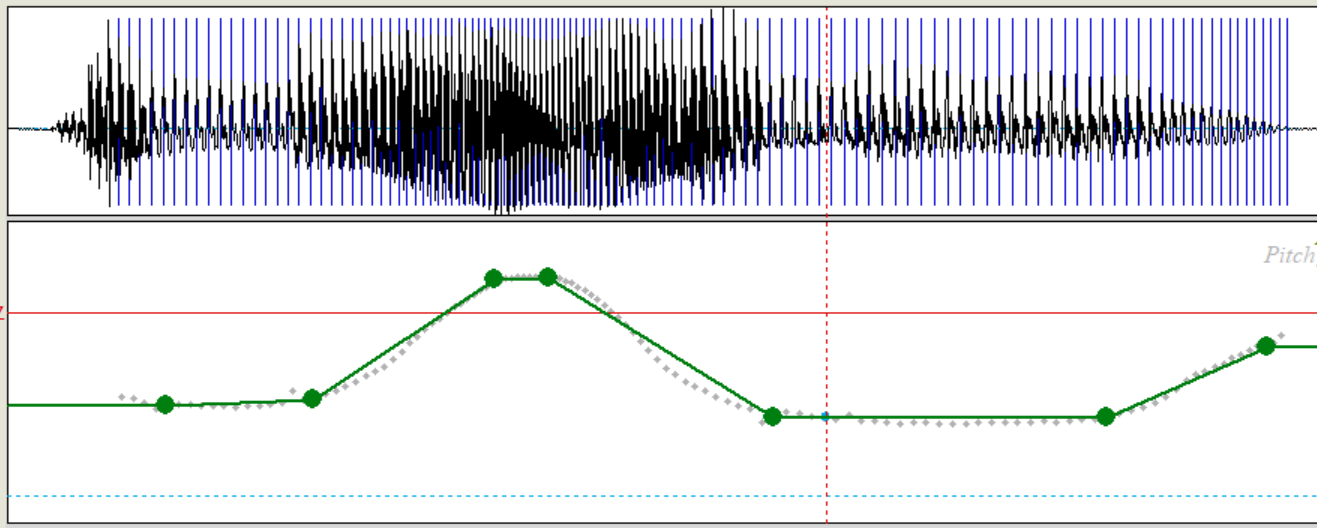
\includegraphics[width=.875\linewidth]{Points-amelia_knew2-resynth-extra.png}
%
\caption[\texttt{amelia\_knew2}, with the resynthesized pitch with an additional point.]{\texttt{amelia\_knew2}, with the resynthesized pitch with an additional point near the f0 peak in green, and the original pitch dotted gray. The addition of the third point makes only an imperceptible change, compared to the resynthesis in the previous figure, and is therefore not needed.%
\label{fig:amelia_knew2 resynth extra}%
}
\end{figure}

As it turns out, these two straight line approximations are perceptually identical. Since the first resynthesis identifies the smaller set of points, and those and only those turning points are perceptually necessary, it is better to label this file with the six turning points in Figure \ref{fig:amelia_knew2 resynth} (and not the seven turning points annotated in Figure \ref{fig:amelia_knew2 resynth extra}). That said, novices should err on the side of over-labelling points as long as they avoid unreliable, noisy f0 points.

One of the contexts where the pitch will often have noisy non-salient turning points is in the case of segmental effects on prosody (“microprosody”). While an experienced labeller may recognize microprosodic perturbations, especially in well known contexts (e.g., around a stop consonant or a sibilant such as [s] or [z]), this may be more difficult for a novice. We will illustrate this briefly here, but the reader is also referred to section \ref{sec:intonational-contours-and-software-based-pitch-tracks} for further discussion. This illustration here concerns the effects of [s]: Compare the pitch tracking surrounding the [s] on “\langtext{nanasanana}” (which was produced with flat pitch, to the point of sounding unnatural) to the pitch tracking of the resynthesized pitch (which sounds identical to the original, to a human ear):

\begin{figure}[H]
\centering
%
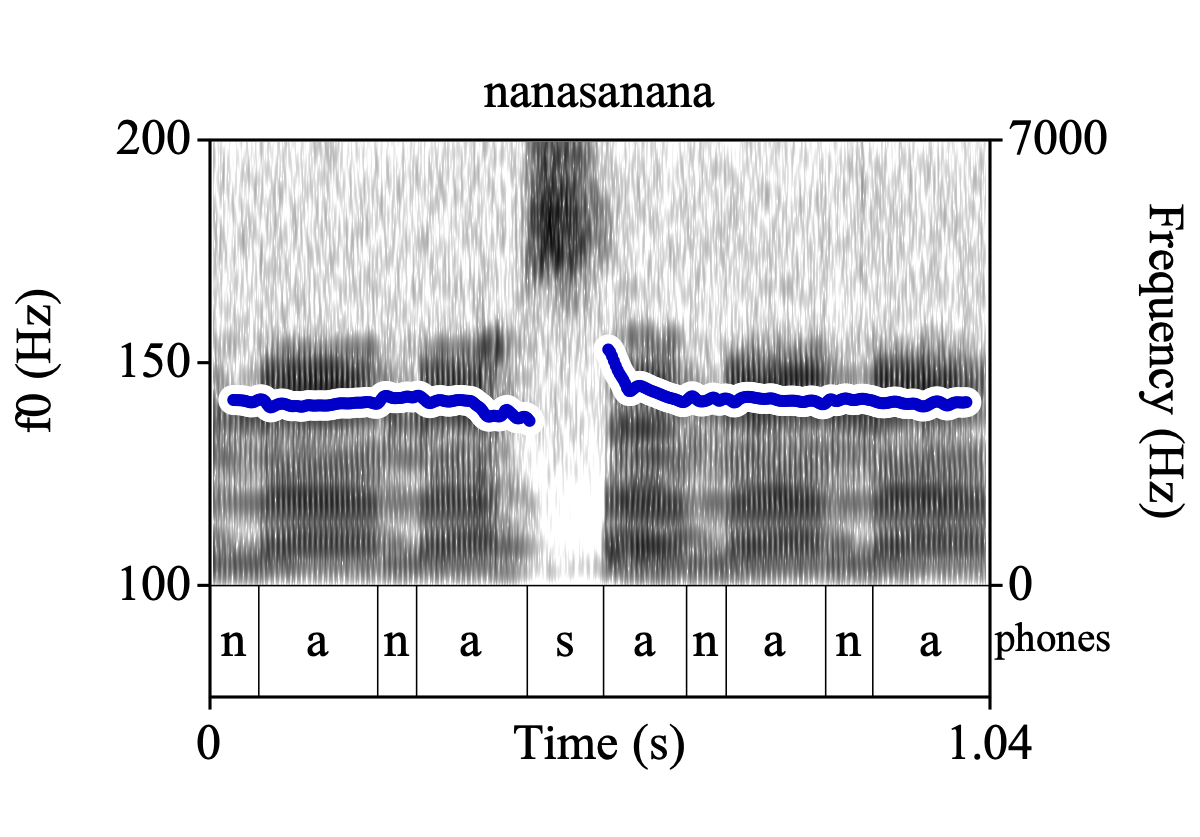
\includegraphics[width=.485\linewidth]{Points-nanasanana.png}~~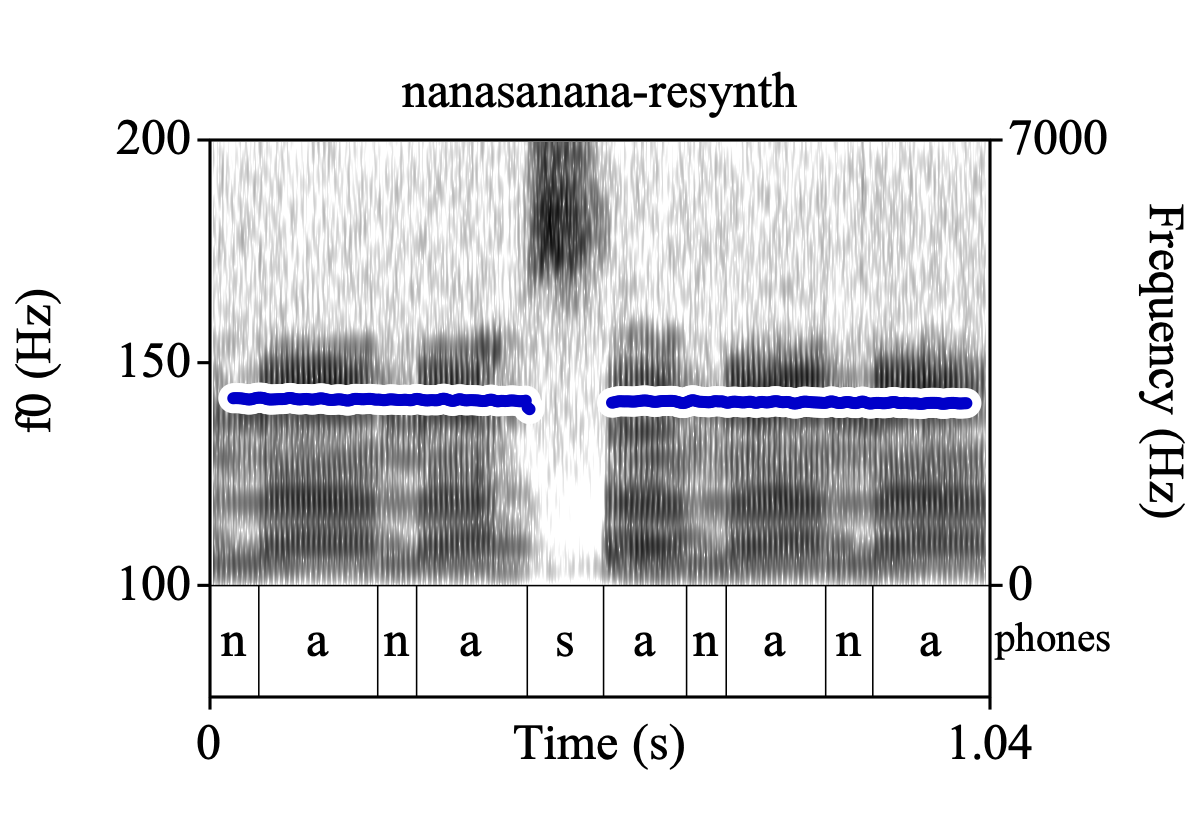
\includegraphics[width=.485\linewidth]{Points-nanasanana-resynth.png}
%
\caption{An original recording (left) and its resynthesized version (right).%
\label{fig:original and resynth}%
}
\end{figure}

The pitch track on the left is the original from Praat. The one on the right has been manipulated and resynthesized in Praat, such that the f0 is a flat line, with the same starting and ending f0 as the original. Listeners generally do not perceive the two audio files in Figure \ref{fig:original and resynth} as different because the f0 movements leading into\slash out of the fricative noise associated with the [s] do not reflect changes in the speaker’s target intonational contour.  Instead, these movements reflect effects of the [s] articulation on the rate of vibration of the vocal folds, and how the software tracks f0. In such cases, where it is clear that the f0 track is influenced by such microprosody, \textbf{the general guideline is to \textit{\uline{not}} put any labels on the Points tier} that would track apparent f0 falls\slash rises that are clearly due to microprosody. In this case, only an initial and final Point would be sufficient to mark the flat f0.

In cases where it is difficult to find \textit{any reliable f0} (e.g., because of microprosodic effects) which may be especially common in the beginning or ends of utterances, section \ref{sec:optional-f0-override-labels-for-annotating-pitch-points-without-a-reliable-f0-track} outlines a solution.

We will return to f0 tracks, intonation contours, and resynthesized straight line approximations in section \ref{sec:intonational-contours-and-software-based-pitch-tracks}.

\subsubsection{Examples of Point Tier labelling}\label{sec:examples-of-point-tier-labelling}

\paragraph{Basic Points Example 1:\label{basic-points-example-1}}

Let us examine a labelled example with a single prominence and a single phrase edge annotated in the Prosodic Structure tier. We will use this example to discuss several aspects of labelling in the Points tier.

\begin{figure}[H]
\centering
%
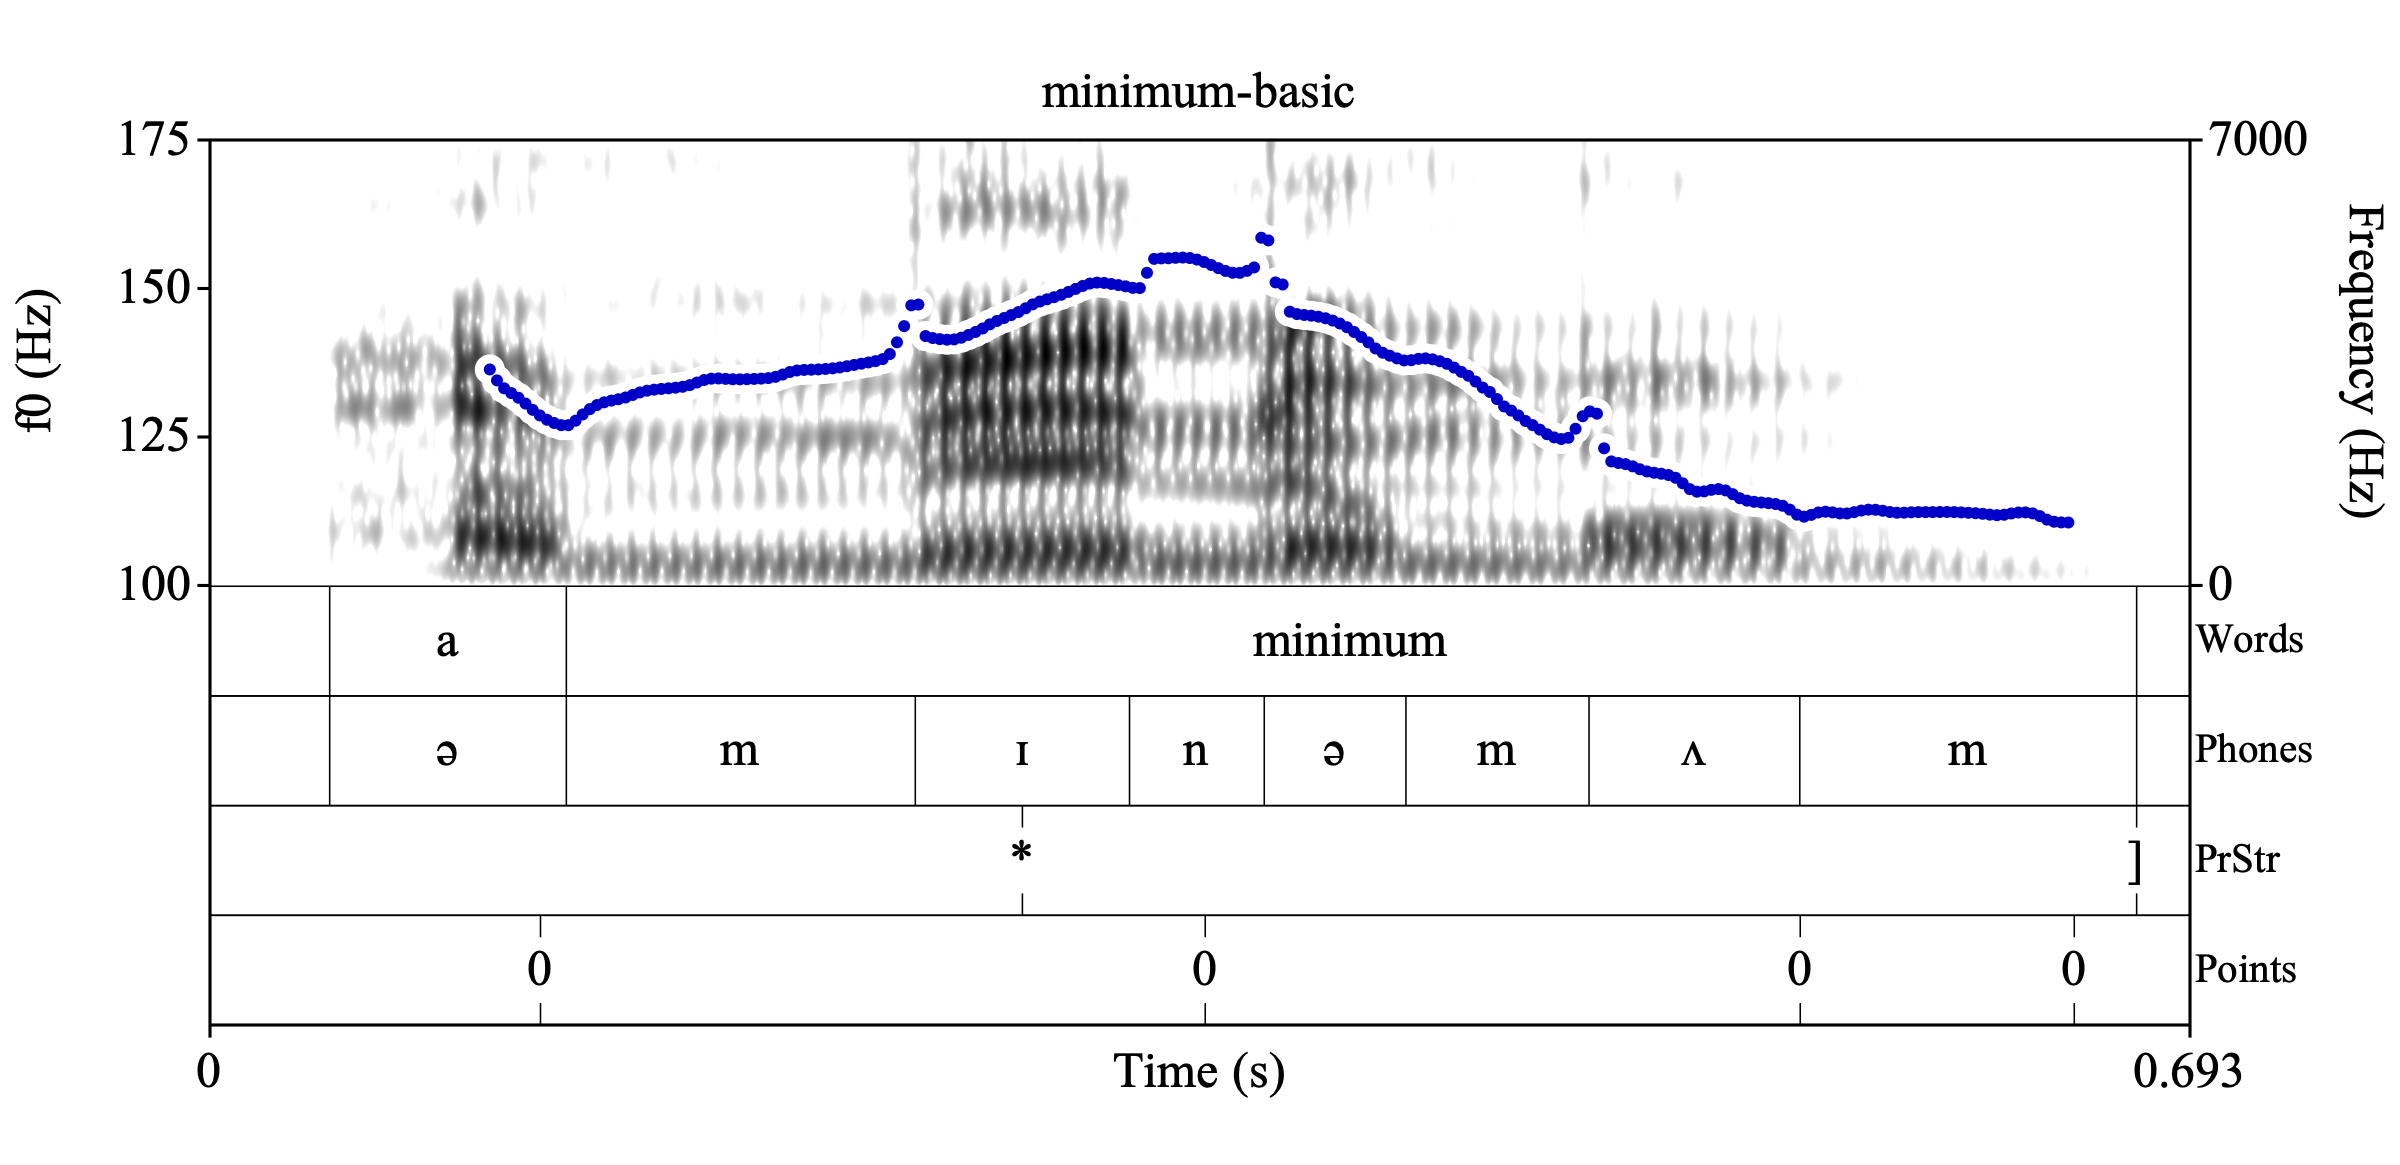
\includegraphics[width=.875\linewidth]{Points-minimum-basic.png}
%
\caption{\texttt{minimum}, with the Points tier annotated with ‘\textlabel{0}’ labels.%
\label{fig:minimum Points basic}%
\index{Annotated example, Points tier (basic)!minimum}%
}
\end{figure}

\uline{First}, note the first (leftmost) ‘\textlabel{0}’ label on the Points tier. It indicates the point in time where (reliable) pitch tracking begins, which corresponds to the beginning of the rise that cues the prominence. (For labellers familiar with other systems like ToBI, take special note that the ‘\textlabel{0}’ default label does not record any relationship between the pitch and the prominence.) Though Praat begins tracking pitch in the middle of “\langtext{a}”, there is no perceptual fall in pitch here, and so we do not want to add a Points label that would produce a falling line at the beginning of the recording. PoLaR labellers are advised to place Points tier labels at the beginning of (reliable) pitch tracking in this way.

\uline{The second ‘\textlabel{0}’ label} is placed at the peak of the f0 track, the location where the pitch again changes direction from rising to falling. Note that the small perturbations between these first two points are not labelled. These are due to noise in the signal processing algorithms and display and are not meaningful in prosodic perception.

\uline{Finally:} The last two points mark the end of the steeper fall and the end of the pitch tract, respectively.

\uline{Overall}, note that the timing of the PrStr tier labels and the timing of the Points labels are completely independent of one another. In the PrStr tier, the \textlabel{*} is aligned to the middle of the stressed vowel, and the \textlabel{]} is aligned to the right edge of the phrase-final word. On the other hand, the Points tier labels are aligned according to the movements of the f0 contour, and not to any particular syllable, word, phrase, etc., and not to any object in the PrStr tier.

\paragraph{Basic Points Example 2:\label{basic-points-example-2}}

In the example in the figure below, the pitch events (rising slightly, falling in two steps) are time-aligned with the default ‘\textlabel{0}’ label.

\begin{figure}[H]
\centering
%
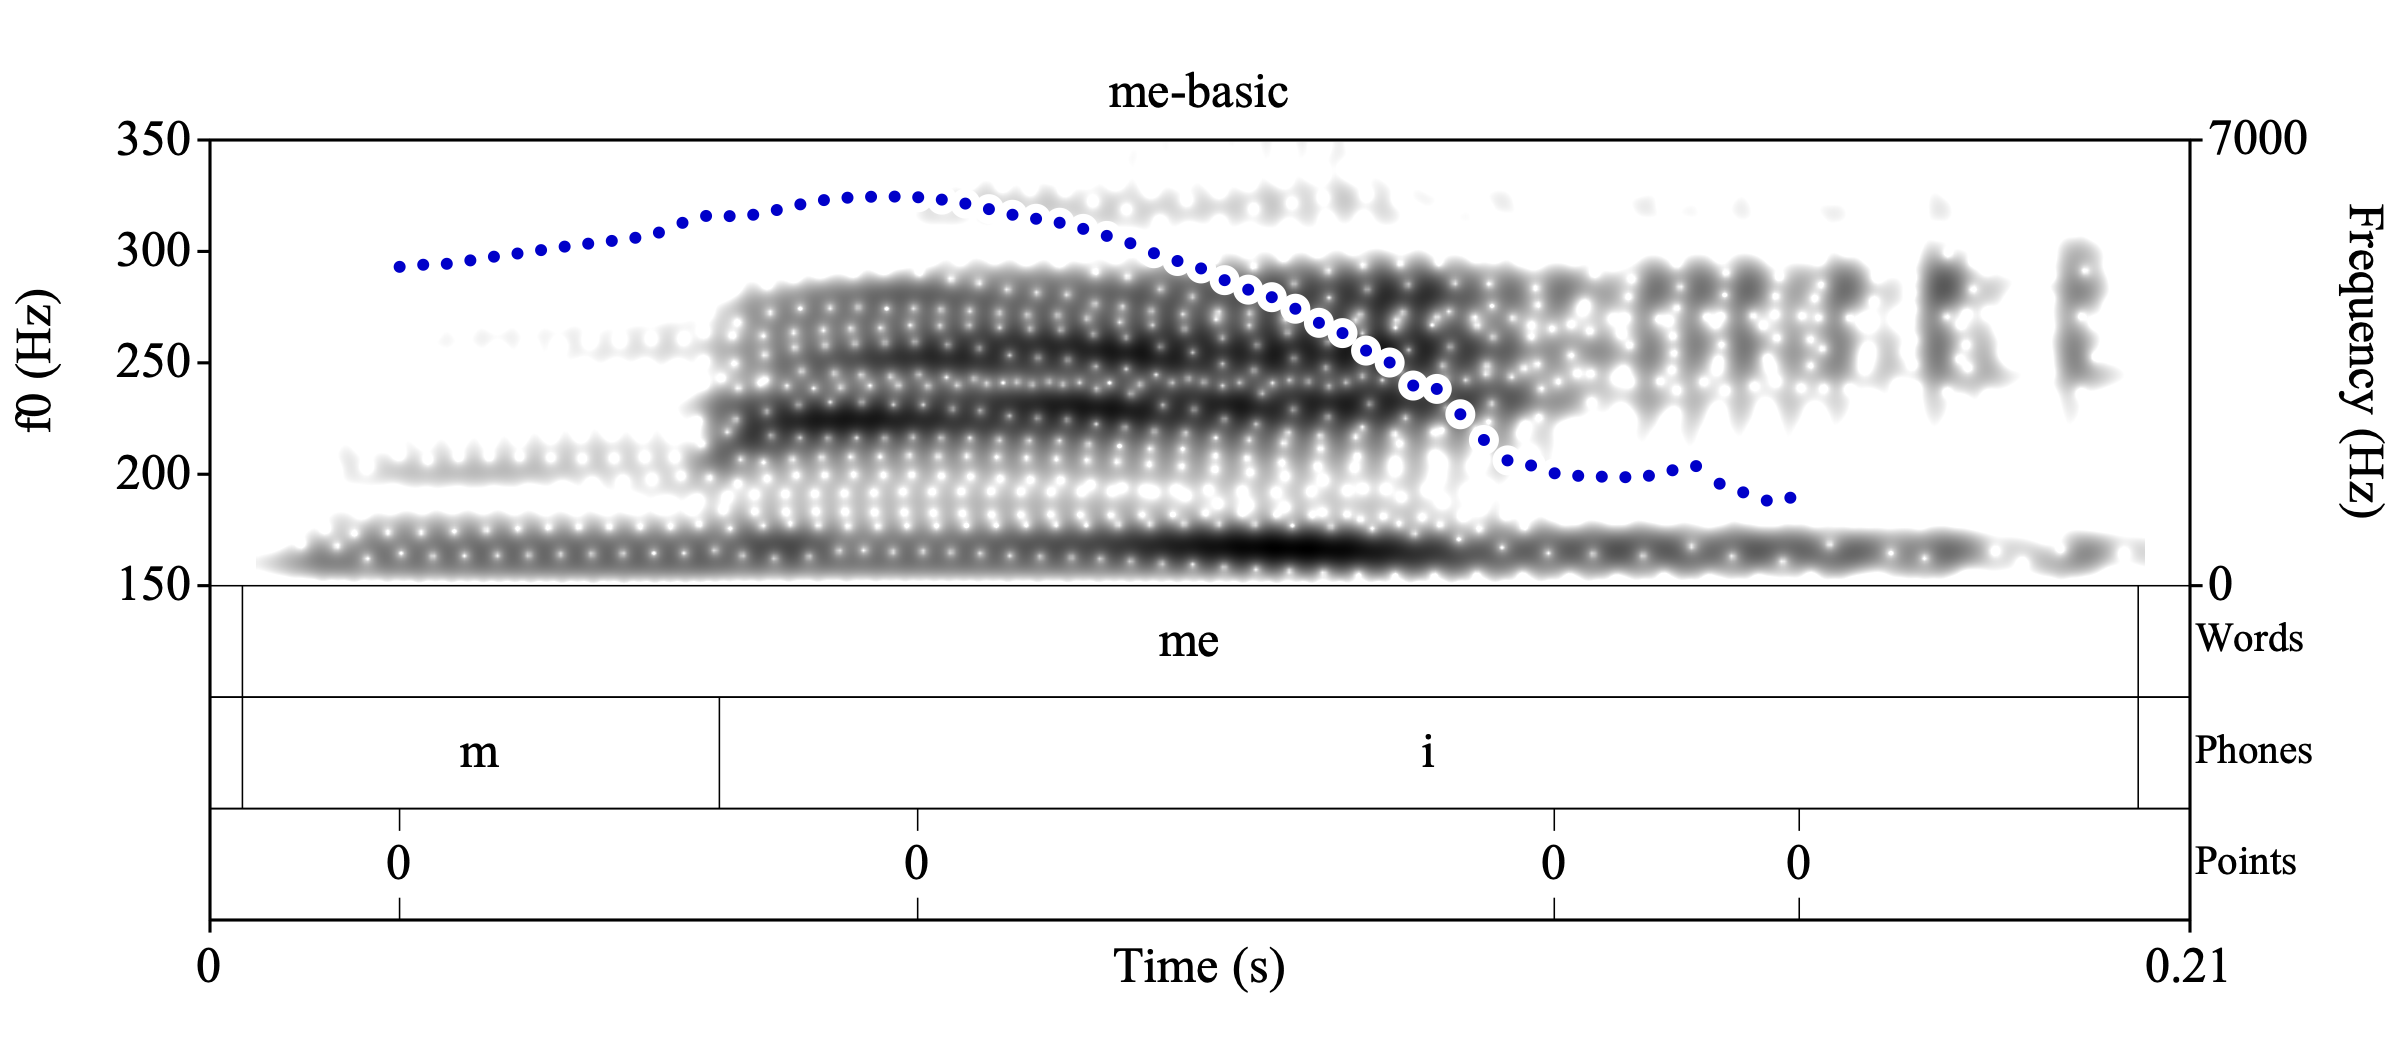
\includegraphics[width=.875\linewidth]{Points-me-basic.png}
%
\caption{\texttt{me}, with the Points tier annotated with ‘\textlabel{0}’ labels.%
\label{fig:me Points basic}%
\index{Annotated example, Points tier (basic)!me}%
}
\end{figure}

Note the timing of the last two labels on the Points tier. The third ‘\textlabel{0}’ occurs where the f0 curve changes trajectory radically, as expected. However, the final ‘\textlabel{0}’ does \textit{\uline{not}} occur at the end of the recording or at the final phrase break (] in the PrStr Tier), because the f0 tracking stops before the recording does. In such a situation, one can simply place the ‘\textlabel{0}’ label where the f0 track ends (or stops being reliable, in the sense of reliably tracking perception of the intonational contour).

\paragraph{Basic Points Example 3:\label{basic-points-example-3}}

Other types of pitch movements might present challenges where the pitch contour displays discontinuities and turns that are not perceptually salient, at least not with respect to the overall perception of the intonation. For example, consider the pitch track below.

\begin{figure}[H]
\centering
%
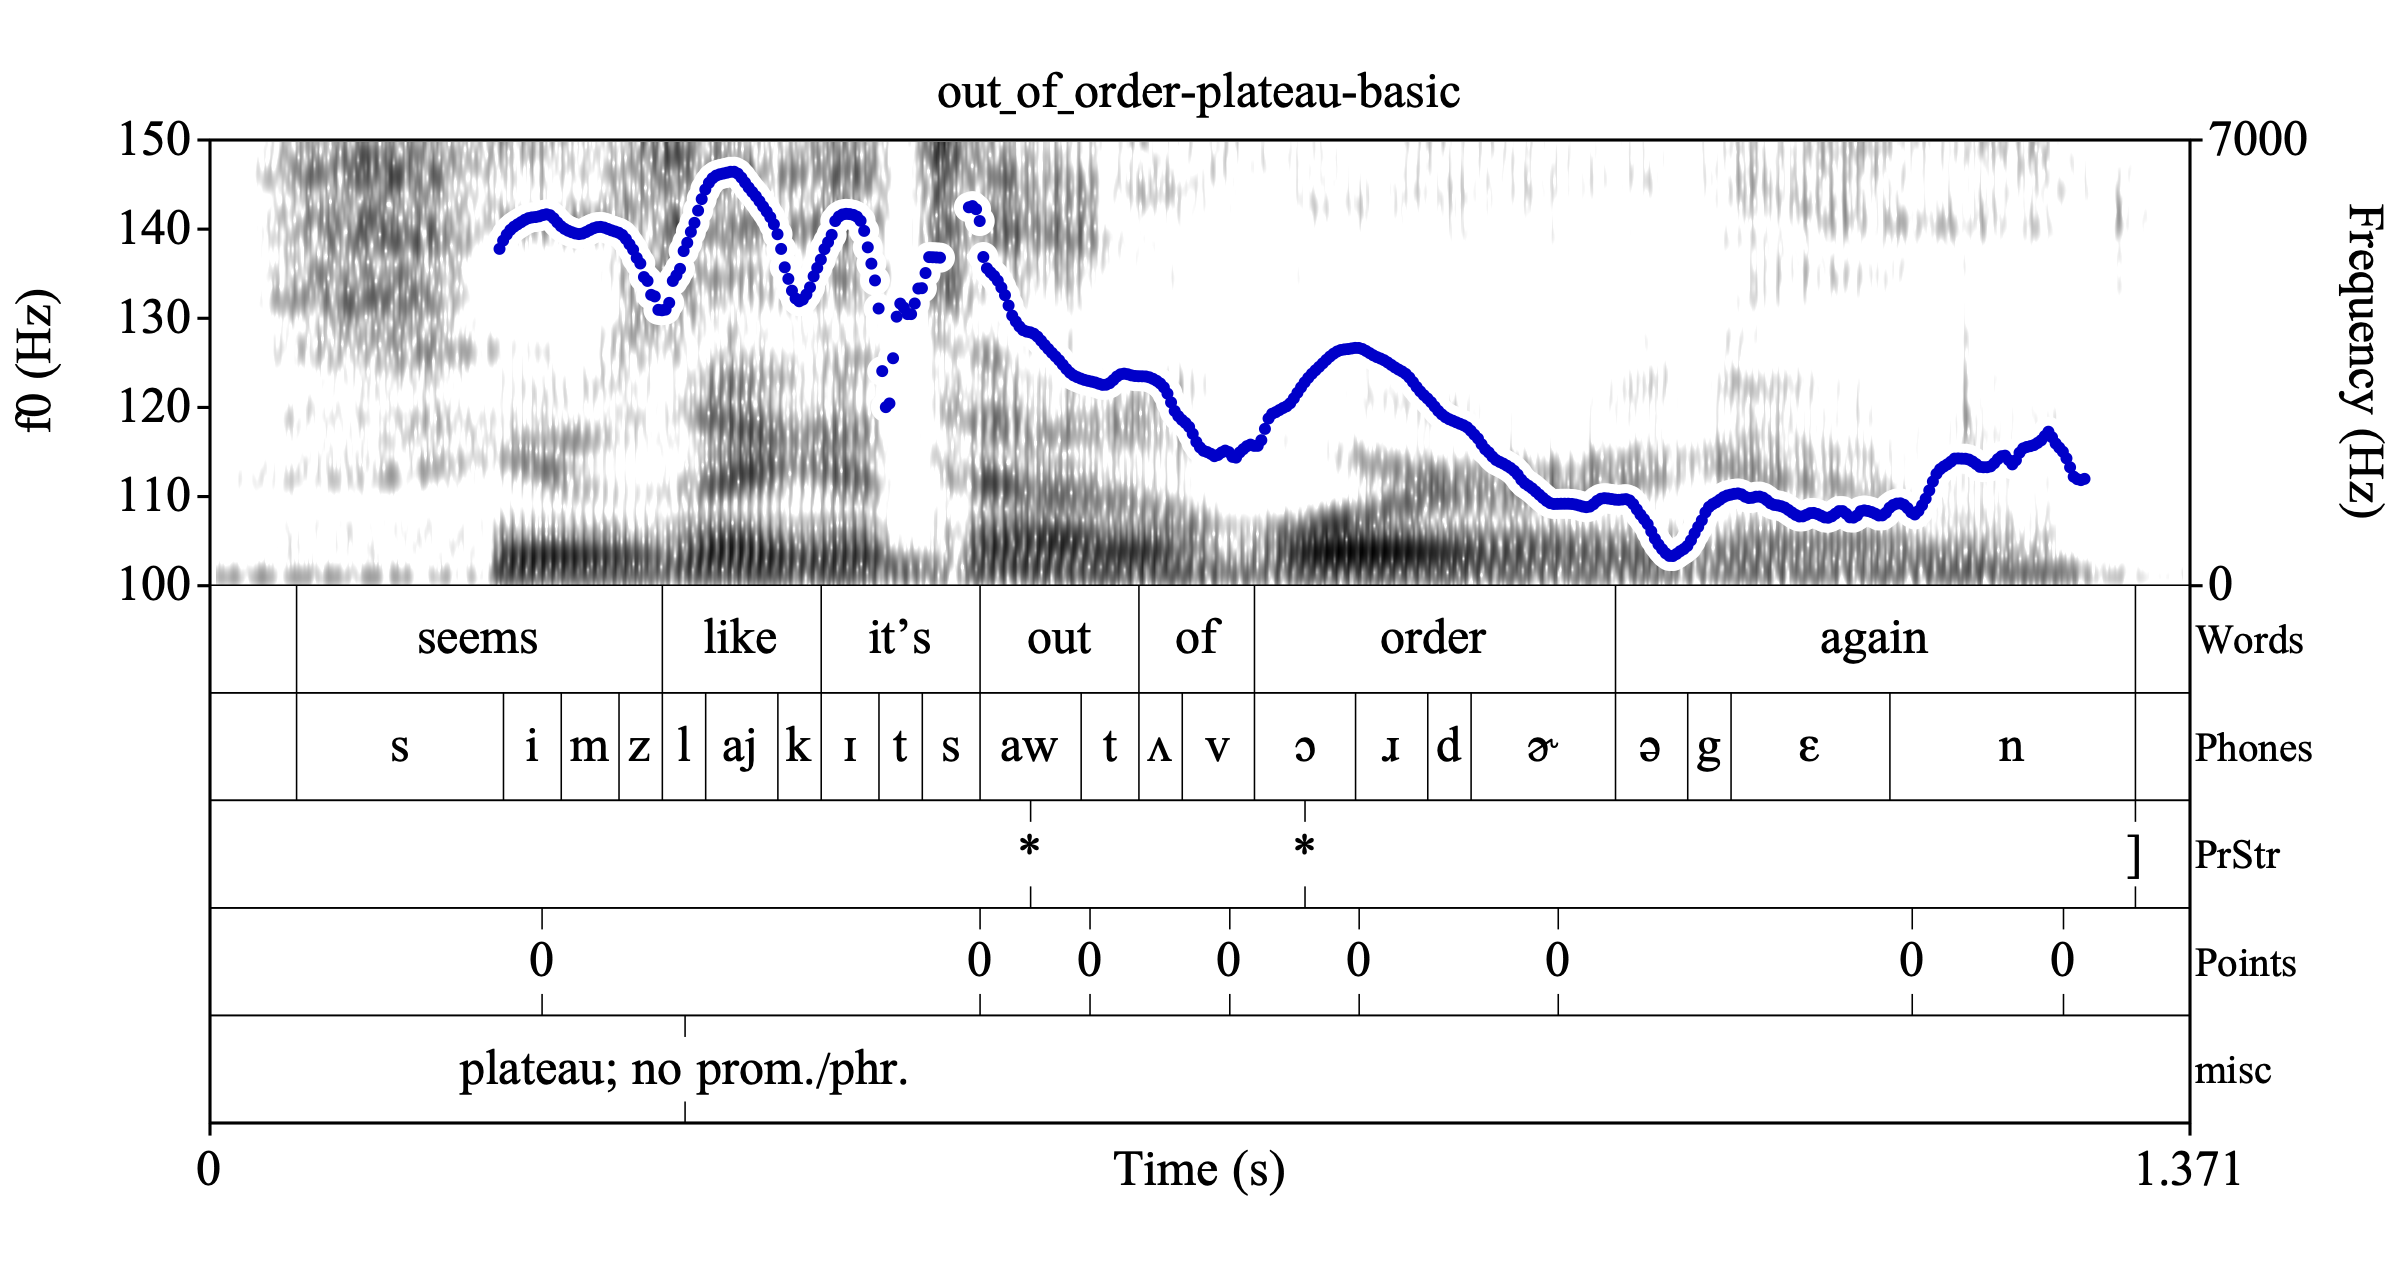
\includegraphics[width=.875\linewidth]{Points-out_of_order-plateau-basic.png}
%
\caption{\texttt{out\_of\_order-plateau}, with the Points tier annotated with ‘\textlabel{0}’ labels.%
\label{fig:out_of_order-plateau Points basic}%
\index{Annotated example, Points tier (basic)!out\_of\_order-plateau}%
}
\end{figure}

Labellers report hearing a steady high pitch at the beginning of the utterance, from “\langtext{seems}” through “\langtext{it’s}” despite the  visible pitch perturbations in the f0-tracking. Moreover, labellers do not perceive any prominence or juncture that would call for a \textlabel{*} or \textlabel{]} label. In order to capture this long, high plateau, points tier labels have to be placed only at the beginning and end  of this interval. This will also reproduce the plateau in a straight line approximation, such as the one created with the PoLaR Praat plugin’s “Resynthesize Straight Line Approximation” command (described in section \ref{sec:identifying-necessary-points-labels-with-straight-line-approximations}), shown in Figure \ref{fig:out_of_order-plateau Points basic resynth}.

\begin{figure}[H]
\centering
%
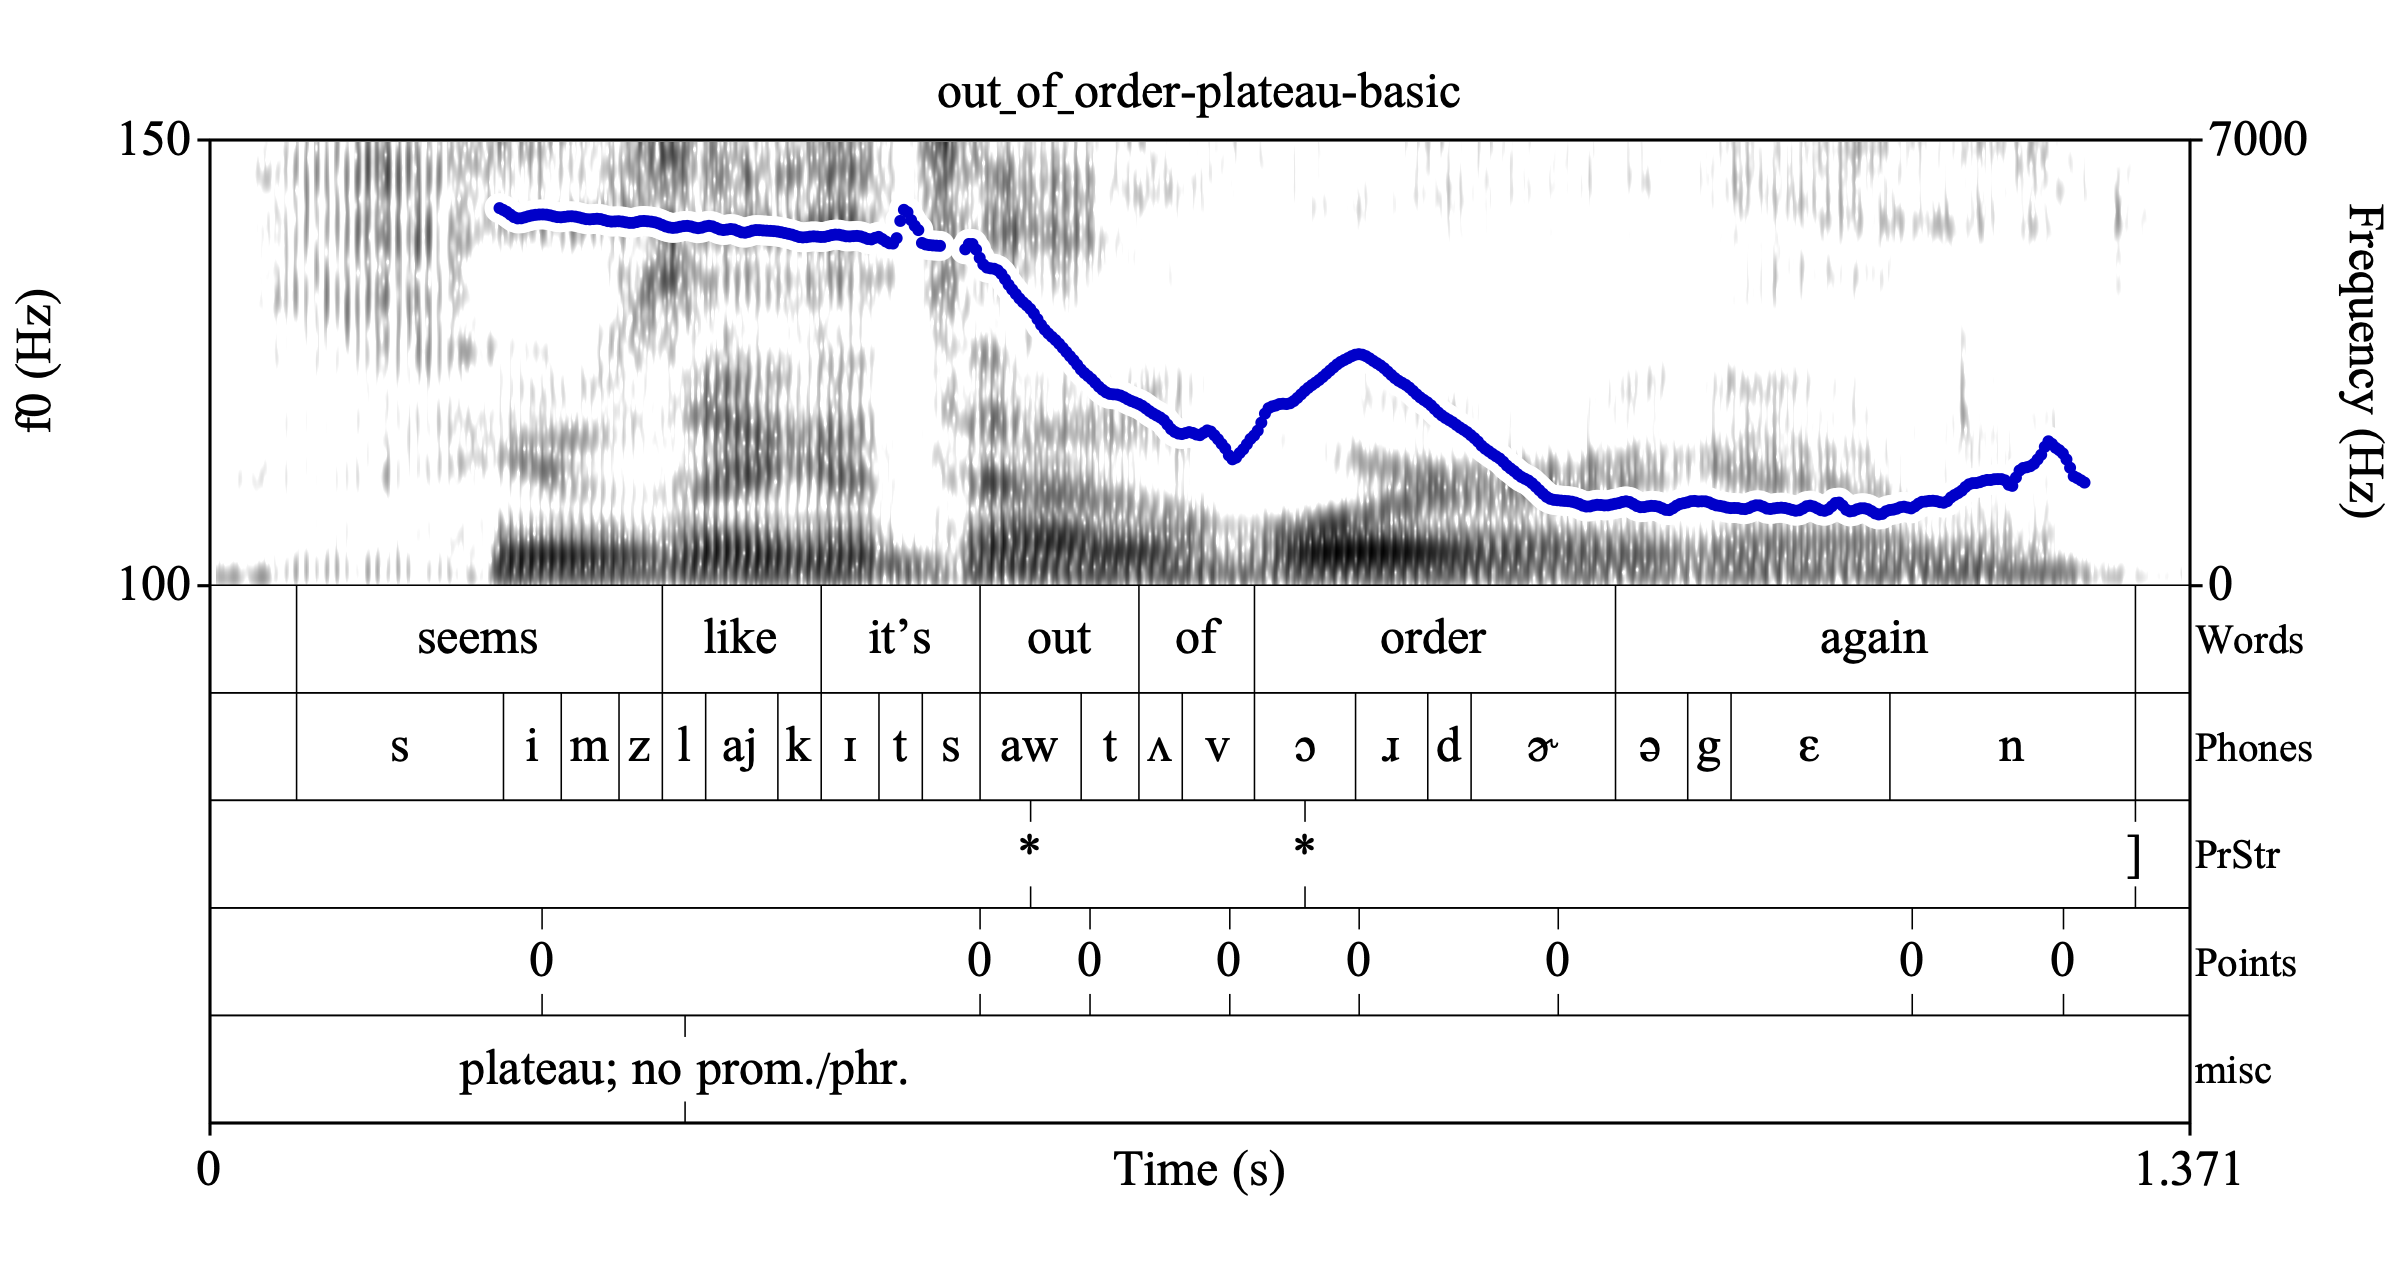
\includegraphics[width=.875\linewidth]{Points-out_of_order-plateau-resynth-basic.png}
%
\caption[\texttt{out\_of\_order-plateau-resynth} is a resynthesized straight-line approximation that is perceived as sounding intonationally the same as the original recording, \texttt{out\_of\_order-plateau}.]{\texttt{out\_of\_order-plateau-resynth} is a resynthesized straight-line approximation that is perceived as sounding intonationally the same as the original recording, \texttt{out\_of\_order-plateau}. (Note that this SLA is not precisely “straight”, despite being resynthesized. This highlights the effect of the signal detection algorithm, even from a source where f0 has been artificially manipulated to consist of straight line segments. Motto: do not place undue trust onto the visual display of the f0 contour.)%
\label{fig:out_of_order-plateau Points basic resynth}%
\index{Annotated example, Points tier (basic)!out\_of\_order-plateau}%
}
\end{figure}

Listeners hear the original recording as sounding intonationally the same as the resynthesized version, corroborating that the pitch tracking in the original recording is unreliable.

With experience, annotators need not resynthesize every turning point to ascertain its validity. In fact, labelling too many turning points is preferable to labelling too few. However, if one were to visually (or with a very simple automatic script) identify all of the f0 turning points in most utterances, there are likely to be more than are necessary to generate an appropriate straight line approximation. Many of these turning points will be typical segmental perturbations or other noise in the signal.

\paragraph{Basic Points Example 4:\label{basic-points-example-4}}

An example of this is below; attend to the fact that there are no Points tier labels in or near the word “\langtext{not}”, (even though it is perceived as prominent):

\begin{figure}[H]
\centering
%
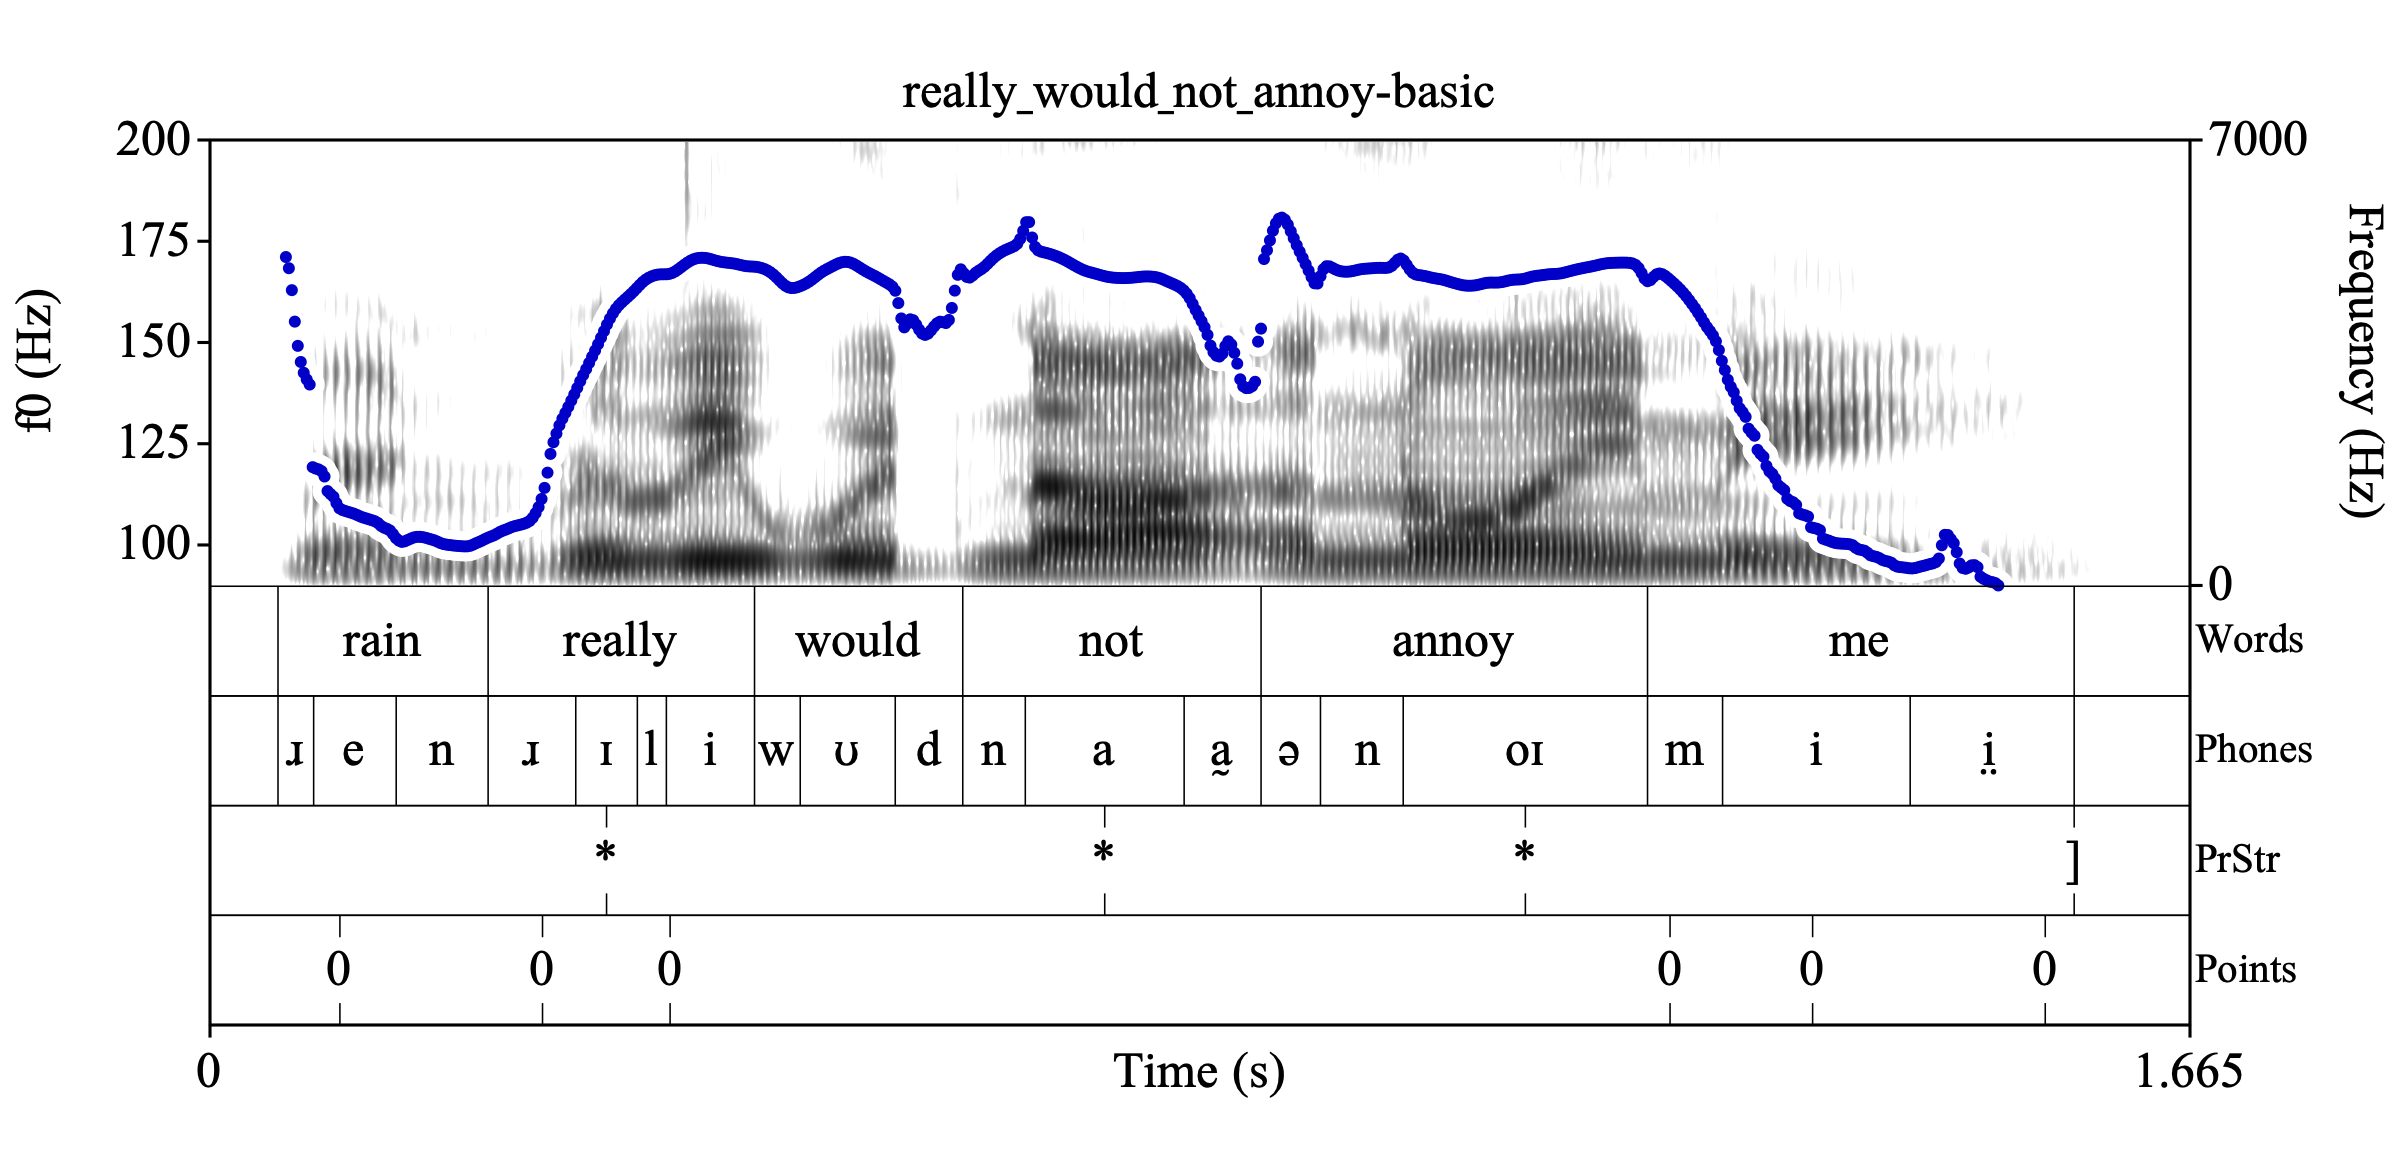
\includegraphics[width=.875\linewidth]{Points-really_would_not_annoy-basic.png}
%
\caption{\texttt{really\_would\_not\_annoy}, with the Points tier annotated with ‘\textlabel{0}’ labels.%
\label{fig:really_would_not_annoy Points basic}%
\index{Annotated example, Points tier (basic)!really\_would\_not\_annoy}%
}
\end{figure}

The small perturbations along the otherwise flat f0 track from “\langtext{really}” through “\langtext{annoy}” are microprosodic or noise related and are also not labelled. Listeners hear this interval as a sustained high tone and not as 2-3 separate peaks. Also note that the leftmost ‘\textlabel{0}’ has been placed at the location of the first reliable f0. In this case, that label is not at the beginning of the f0 tracking; instead, its placement is meant to indicate that the labeller does not believe that f0 track produced by the software is accurate until a bit into the vowel of “\langtext{rain}”.


\subsubsection{Labeller Uncertainty}\label{sec:labeller-uncertainty-points}

As was the case when labelling prosodic events in the PrStr Tier, labellers might be uncertain about whether an f0 turning point exists. In many of these cases, using the Straight Line Approximation Tool or the Override Labels described in the next section can resolve these issues. However, if neither approach is helpful, the labeller can again employ the ‘\textlabel{?}’ (as in ‘\textlabel{?0}’) to indicate that there might be a turning point at this location but it is not certain.

\subsubsection{Optional f0 Override Labels for Annotating Pitch Points without a (Reliable) f0 Track}\label{sec:optional-f0-override-labels-for-annotating-pitch-points-without-a-reliable-f0-track}

At this point, we have discussed how software-produced f0 tracks may not have a direct correspondence to pitch perception (as in, e.g., cases where the f0 tracking disappears or jumps around). In this section we describe a method that a labeller can use to address this problem, by adding a Points label that can be informative for later analysis.

There are multiple reasons why a pitch track may be discontinuous or display faulty f0 points. First, f0 is the measurement of the vocal fold vibration rate (“voicing”) and there are naturally occurring speech events where the vocal folds don’t vibrate (e.g., voiceless segments such as [f]) or they vibrate irregularly (“creaky” voice). While this produces gaps in regular vocal fold vibration, many of these are “corrected for” by the human perceiver, who perceives the pitch as continuous and steady.

In addition, the f0 pitch tracking display itself (in software like Praat) might be inaccurate due to the software f0-tracking settings. Most speech applications require some calibration for each speaker, so that f0 displays are as accurate (and as easily read) as possible. For example, inappropriate settings for the maximum f0 value and/or the minimum f0 value under Praat’s “Pitch settings” can lead to pitch halving\slash doubling (in which the reported f0 value is half or double of the “true” value), while inappropriate settings for the voicing threshold and octave jump costs can lead to f0 dropout or spurious f0 readings.

Lastly, there may also be portions of a recording where there is interference from environmental\slash recording factors, disrupting the f0 tracking algorithms.

These are just some of a few reasons that a pitch track may not always be reliable. (For further discussion of these phenomena, and examples of them, see section \ref{sec:intonational-contours-and-software-based-pitch-tracks}.) At the same time, it is sometimes the case that a labeller can induce where the pitch track “should” be, even when automatic f0 estimates are misleading or f0 cannot be measured at all. This induction is possible because of the way human speech perception works (as mentioned above), and it is aided by visual tools like (partial) f0 tracks that the software can provide. \textbf{To put it more briefly: it is possible that a labeller may have an intuitive sense of where (in time and frequency) a pitch turning point sits, better than the f0 tracking software.}

For this reason, PoLaR provides a means for a labeller to “override” the f0 tracking, and annotate the f0 value that they intuit in the Points label. To annotate this, the labeller adds a comma and the intuited f0 value after the Points label: for example, ‘\textlabel{0,98}’ on the Points tier indicates there is a pitch turning point at this time, and the f0 should be treated as 98Hz (instead of whatever f0 value the software tracker finds). Examples of these “\textbf{comma override}” labels on the Points tier are provided below.

Before getting to the examples, let’s review three reasons that these comma annotations should be used.
\begin{enumerate}
	\item One reason to use them is to ensure that future analysis of the f0, which runs on the basis of PoLaR labels, is reliable. (That is, to minimize misleading measurements that result from f0 tracking errors.)
	\item A second, related reason is that f0 at the end of an utterance is very often creaky and therefore unreliable; thus a Points label without a comma override value might lead to inappropriate f0 values, leading to issues with analysis, straight line approximation resynthesis, etc.
	\item The last, somewhat practical  reason is that various PoLaR scripts and tools, such as the straight-line approximation resynthesizer (described in \ref{sec:identifying-necessary-points-labels-with-straight-line-approximations}), are much less useful if they resynthesize on the basis of unreliable or missing f0 measurements.
\end{enumerate}

A brief note is in order about the PoLaR straight-line approximation resynthesis tool: it always uses override values where they exist (preferring the override value over whatever value Praat estimates for f0). As a result, the annotator can use this tool to “check their work” to see if the override values are appropriate, by perceptually comparing the original sound file and the resultant straight-line approximation. If the two sound essentially the same (modulo minor distortions inherent in resynthesis), the override labels are likely valid. If they do not sound the same, the labeller ought to try adjusting the values in any comma override annotations (as well as the timing of their Points tier labels).

\paragraph{Pitch Override Points Example 1: Unreliable f0 in creaky voice\label{pitch-override-points-example-1}}

Consider the following case, where the pitch track is unreliable during “\langtext{out there}” due to issues of phonation. In this case, there is creaky voice (or silence) for most of the interval, and creaky voice can seriously impede the f0 detection algorithm and lead it to incorrect f0 estimates.



\begin{figure}[H]
\centering
%
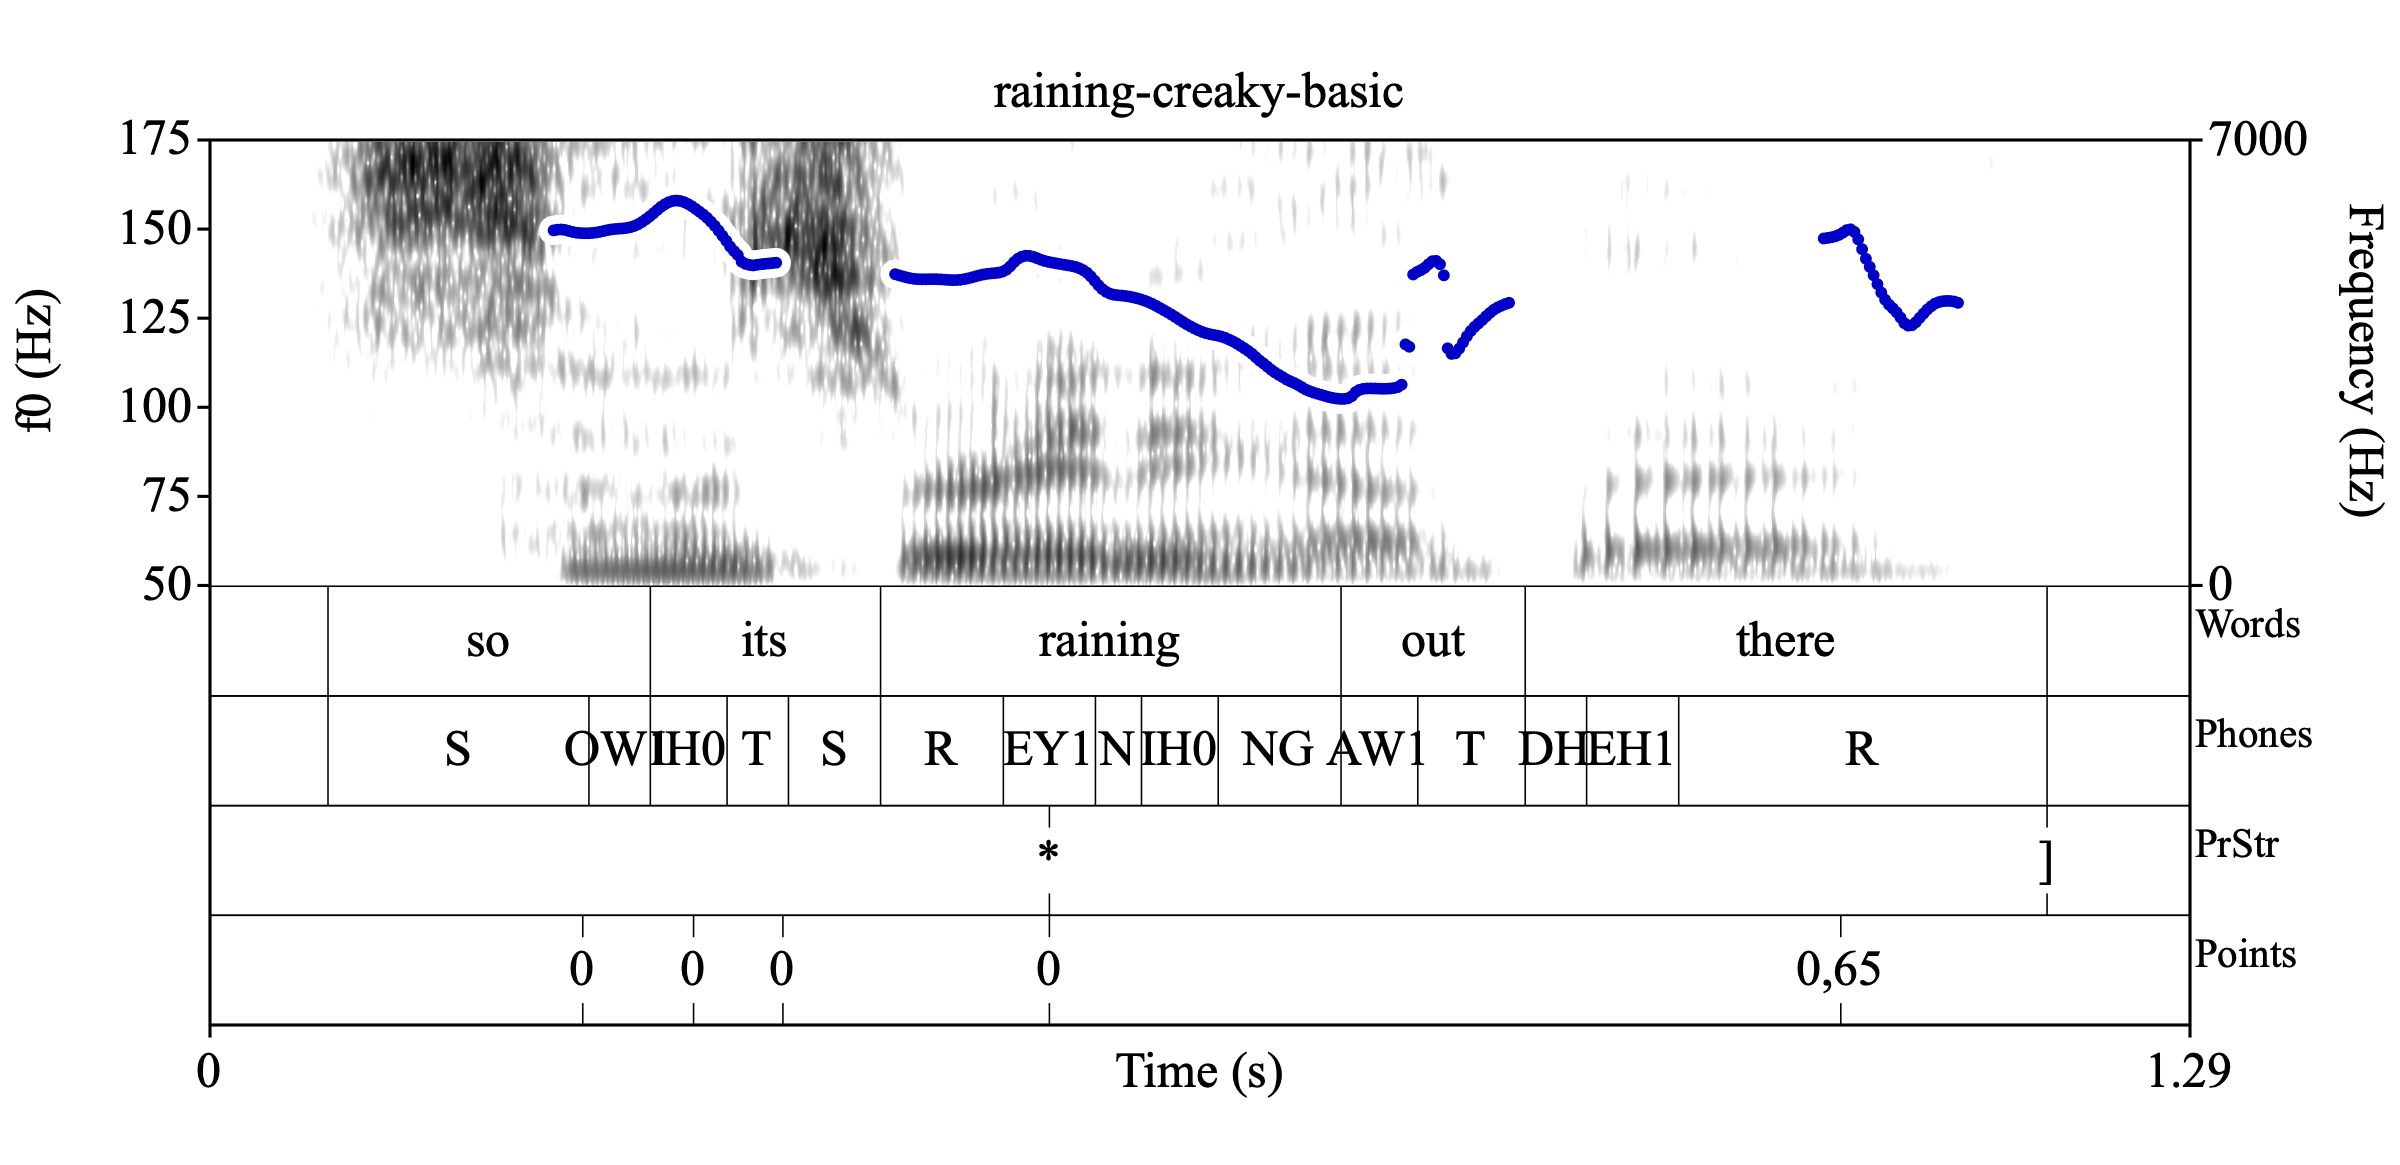
\includegraphics[width=.875\linewidth]{Points-raining-creaky-basic-comma.png}
%
\caption{\texttt{raining-creaky}, with the f0 override PoLaR labels.%
\label{fig:raining-creaky Points comma}%
\index{Annotated example, PrStr tier (basic)!raining-creaky}%
}
\end{figure}

Here, the labellers heard the pitch falling steadily from the stressed vowel of “\langtext{raining}” to the end of the utterance, and estimated that the pitch at the end point of the fall should be about 65Hz (arriving at this number using a methodology described below). Since the initial f0 contour is reliable in this example, the initial ‘\textlabel{0}’ labels don’t need the help of the comma override. A resynthesized straight line approximation of this pitch, that perceptually matches the original, verifies there is no turning point near “\langtext{out}” even though the original software-generated f0 track (above) suggests there might be. This straight line approximation is shown in Figure \ref{fig:raining-creaky Points basic resynth}.

\begin{figure}[H]
\centering
%
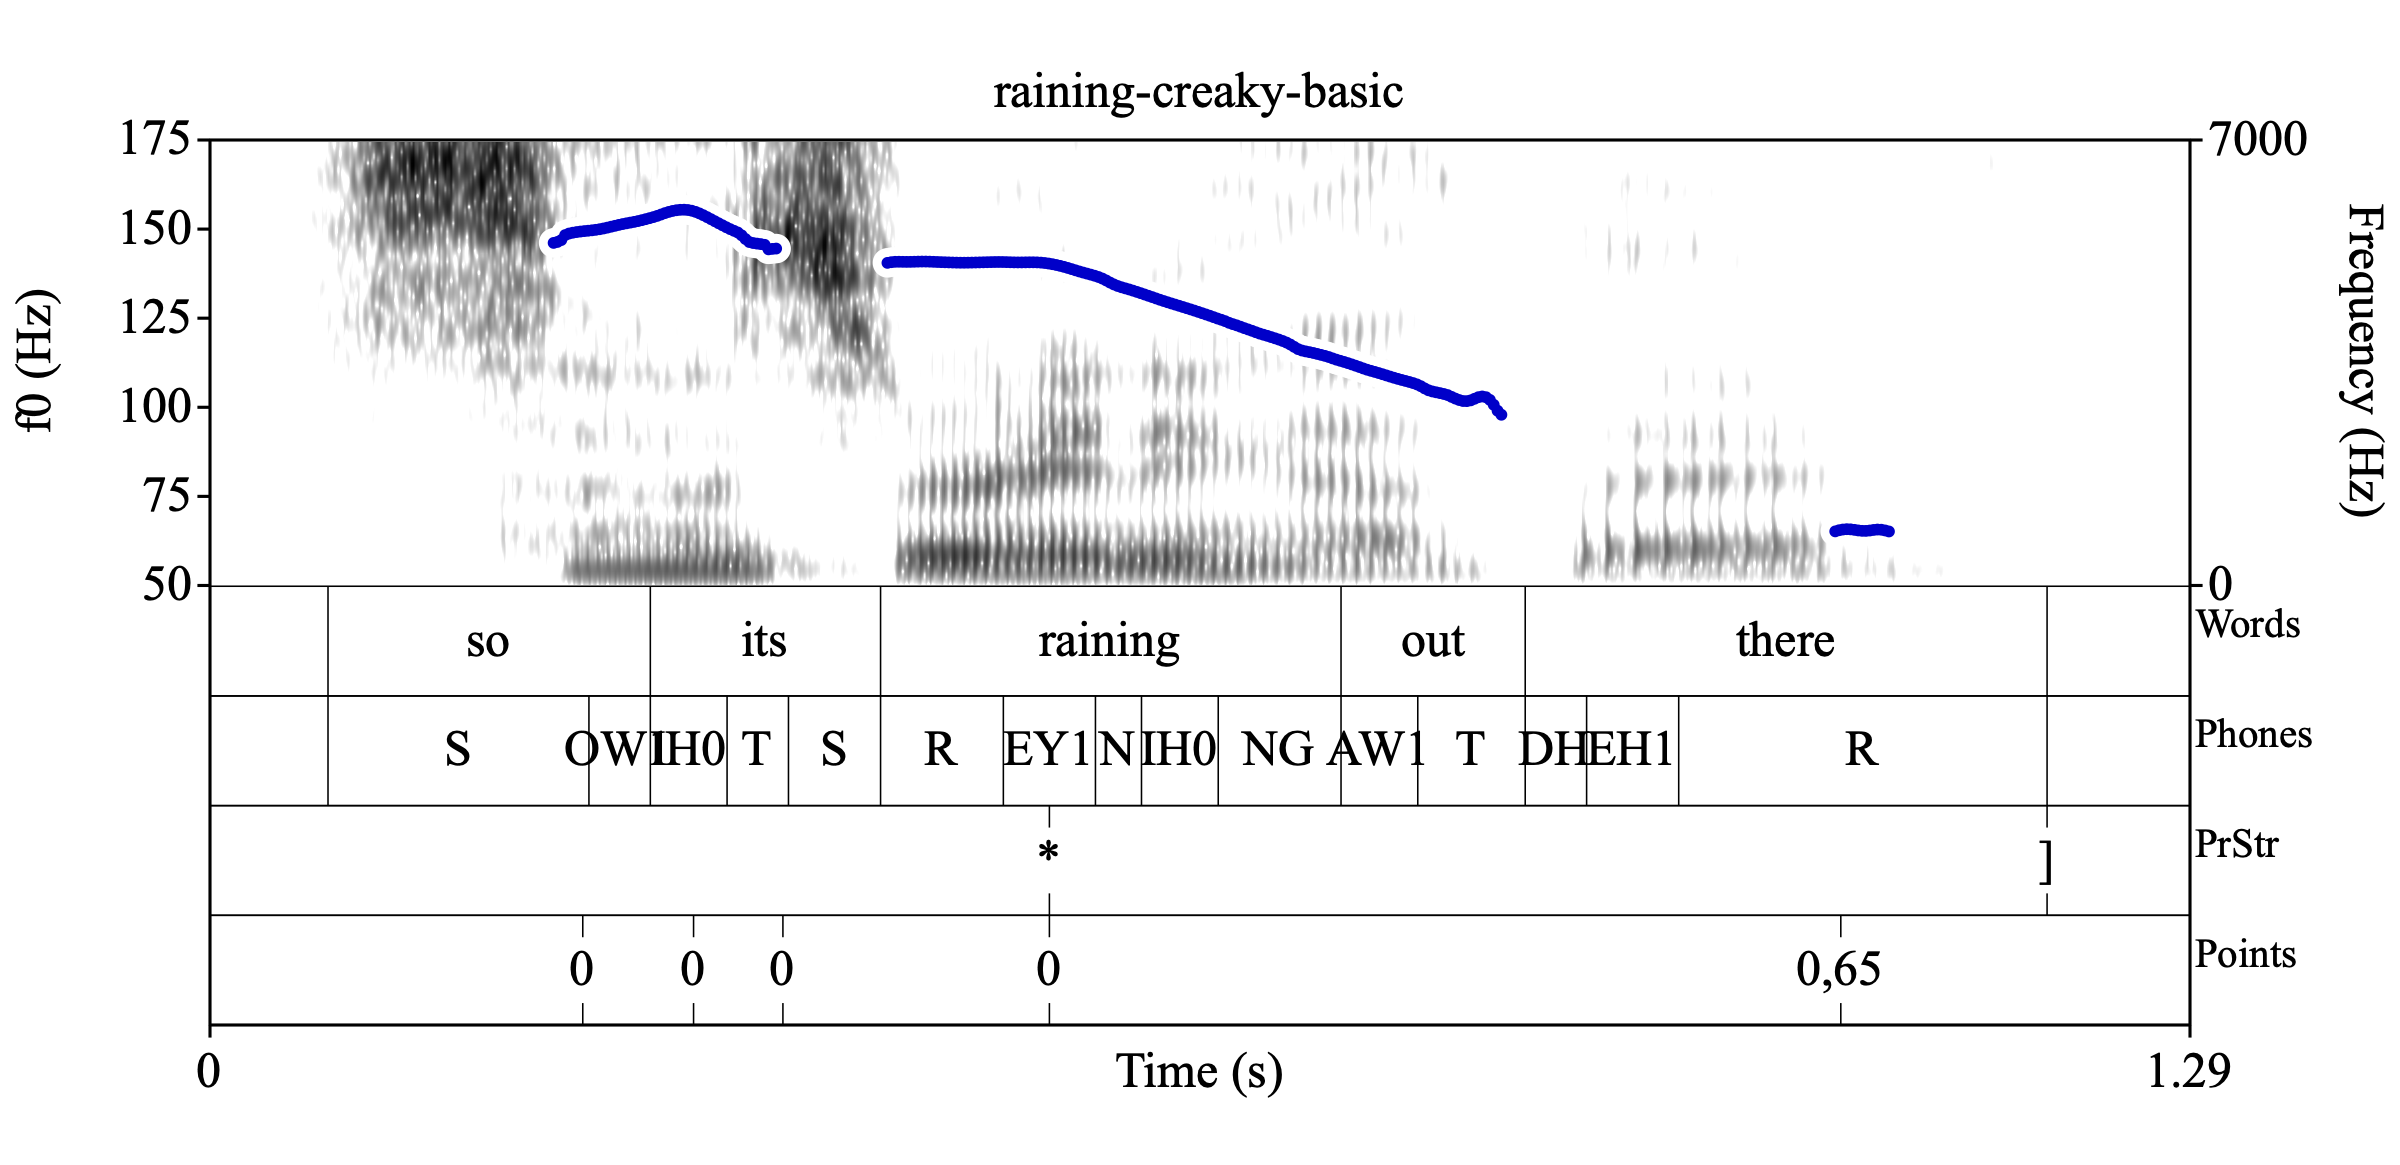
\includegraphics[width=.875\linewidth]{Points-raining-creaky-resynth-basic.png}
%
\caption{\texttt{raining-creaky-resynth} is a resynthesized straight-line approximation that is perceived as sounding intonationally the same as the original recording, \texttt{raining-creaky}.%
\label{fig:raining-creaky Points basic resynth}%
\index{Annotated example, Points tier (basic)!raining-creaky}%
}
\end{figure}

In cases like this (especially with creaky voice, which is so pervasive), labellers are encouraged to provide a guess at comma override values, resynthesize (with the Resynthesize Straight Line Approximation tool), and listen\slash compare the original and resynthesis. It may take several iterations of this, with different guesses at appropriate comma override values before the resynthesis sounds appropriately equivalent. (In cases where it is especially challenging or the labeller is uncertain about their comma overrides, they are encouraged to add a note to the Misc tier indicating this.) 

\paragraph{Pitch Override Points Example 2: End of an utterance\label{pitch-override-points-example-2}}

In a second case, the pitch tracking for the boundary-related tones is unreliable at best (in part because of non-modal phonation beginning in “\langtext{order}” and lasting through the end of “\langtext{again}”). Notice that though there are some valleys in “\langtext{of}” and the beginning of “\langtext{order}”, there are no perceptible falls in pitch there (as confirmed by the straight line approximations achieved through pitch resynthesis). The pitch flattens out during again, though there is a slight perceptible rise (this may have to do with the switch from creaky to breathy phonation); because the f0 tracking is unreliable, as is often the case at the ends of an utterance, the f0 values are hard-coded into the final two Points labels.

\begin{figure}[H]
\centering
%
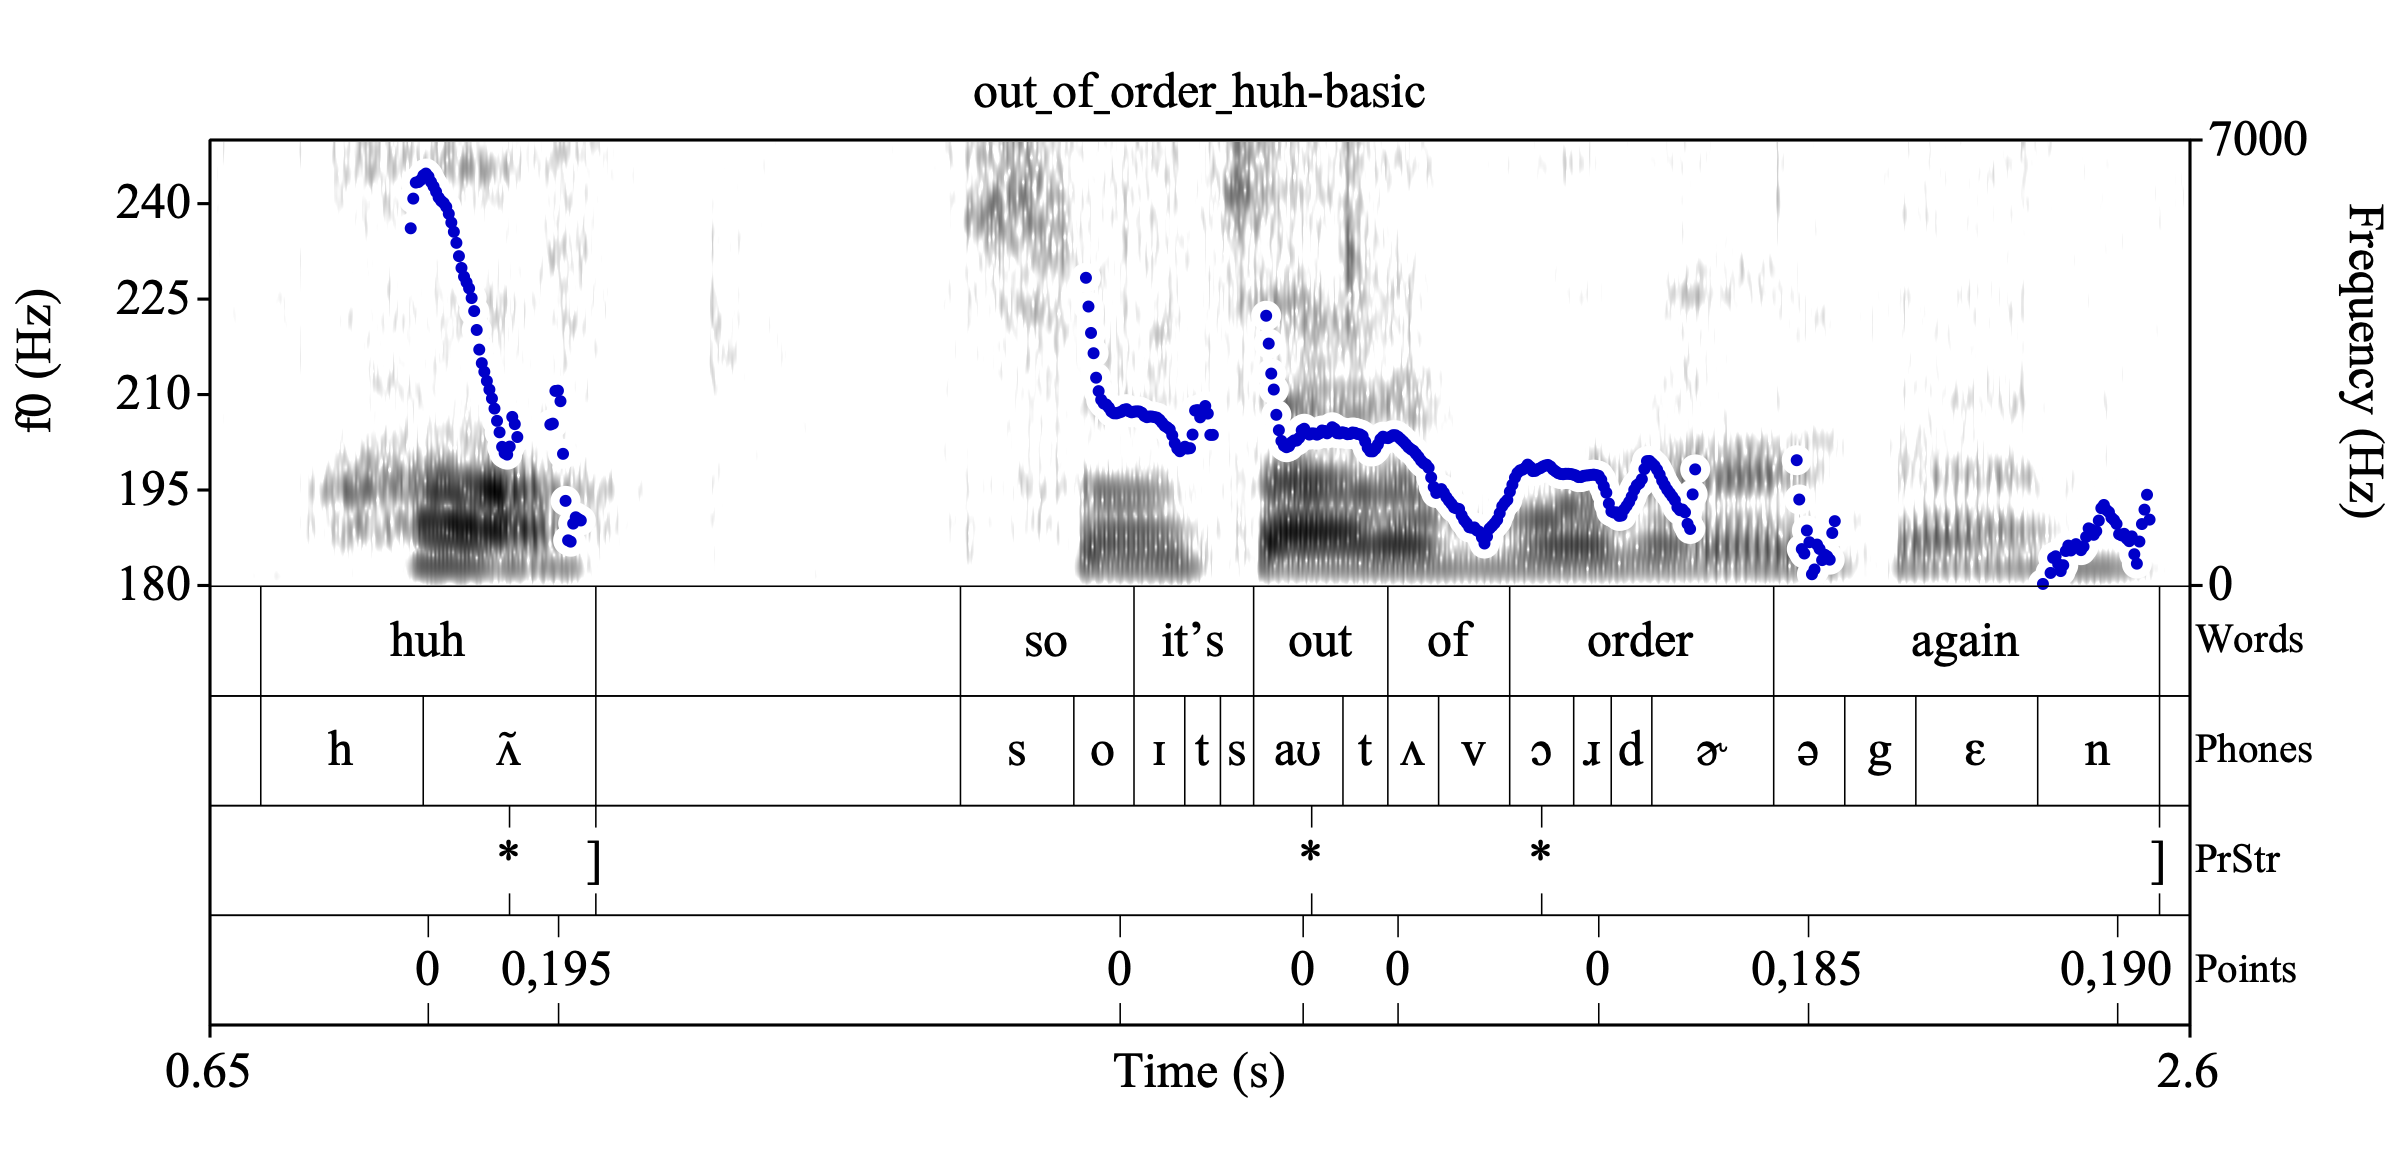
\includegraphics[width=.875\linewidth]{Points-out_of_order_huh-basic-comma.png}
%
\caption{\texttt{out\_of\_order\_huh}, with f0 override PoLaR labels.%
\label{fig:out_of_order_huh Points comma}%
\index{Annotated example, Points tier (basic)!out\_of\_order\_huh}%
}
\end{figure}

The f0 is unreliable in many locations. Using ‘\textlabel{0}’ (as we do for utterances at the beginning and end, respectively, of reliable f0) would not capture valuable information about the falls. 
%todo this is commented out… revisit this
%However, a labeller can approximate where in time the pitch reaches a particular frequency (based on auditory perception\slash visual cues from the pitch track), and the approximate value for that frequency (based on surrounding pitch tracking that appears to be reliable). PoLaR allows the annotator to include in the label what the pitch value “should be”, based on their intuitive\slash inferential abilities by appending a second label on the Points tier, using a comma delimiter followed by the f0 estimate. In the first label i
In this example, ‘\textlabel{0,195}’ indicates “This turning point is associated with a phrase boundary object time-aligned after this point, on the Prosodic Structure tier. The pitch value for this point should be 195Hz.” Thus the ‘\textlabel{,195}’ portion of the label overrides the f0-track (which lacks a pitch value at this point) and can be extracted as a replacement in later processing, such as comparing slopes of f0 movements.

This sort of “manual override” is not just for cases where f0 is absent but can be used for unreliable f0 as is the case with the final two turning points. The labeller judges that the last f0 interval is a mostly flat, rising from 185Hz to 190Hz, and uses ‘\textlabel{0,185}’ and ‘\textlabel{0,190}’ at each end to override whatever f0 value the pitch tracking software provides.

\paragraph{Pitch Override Points Example 3: Missing f0 values in voiceless speech\label{pitch-override-points-example-3}}

The case above is for a phrase end where pitch tracking is often unreliable, but this method of directly annotating pitch value approximations can be used for any Points tier object where the labeller is concerned that pitch tracking might not be reliable. Consider the example below, which contains three Points tier objects with manual-override pitch values:

\begin{figure}[H]
\centering
%
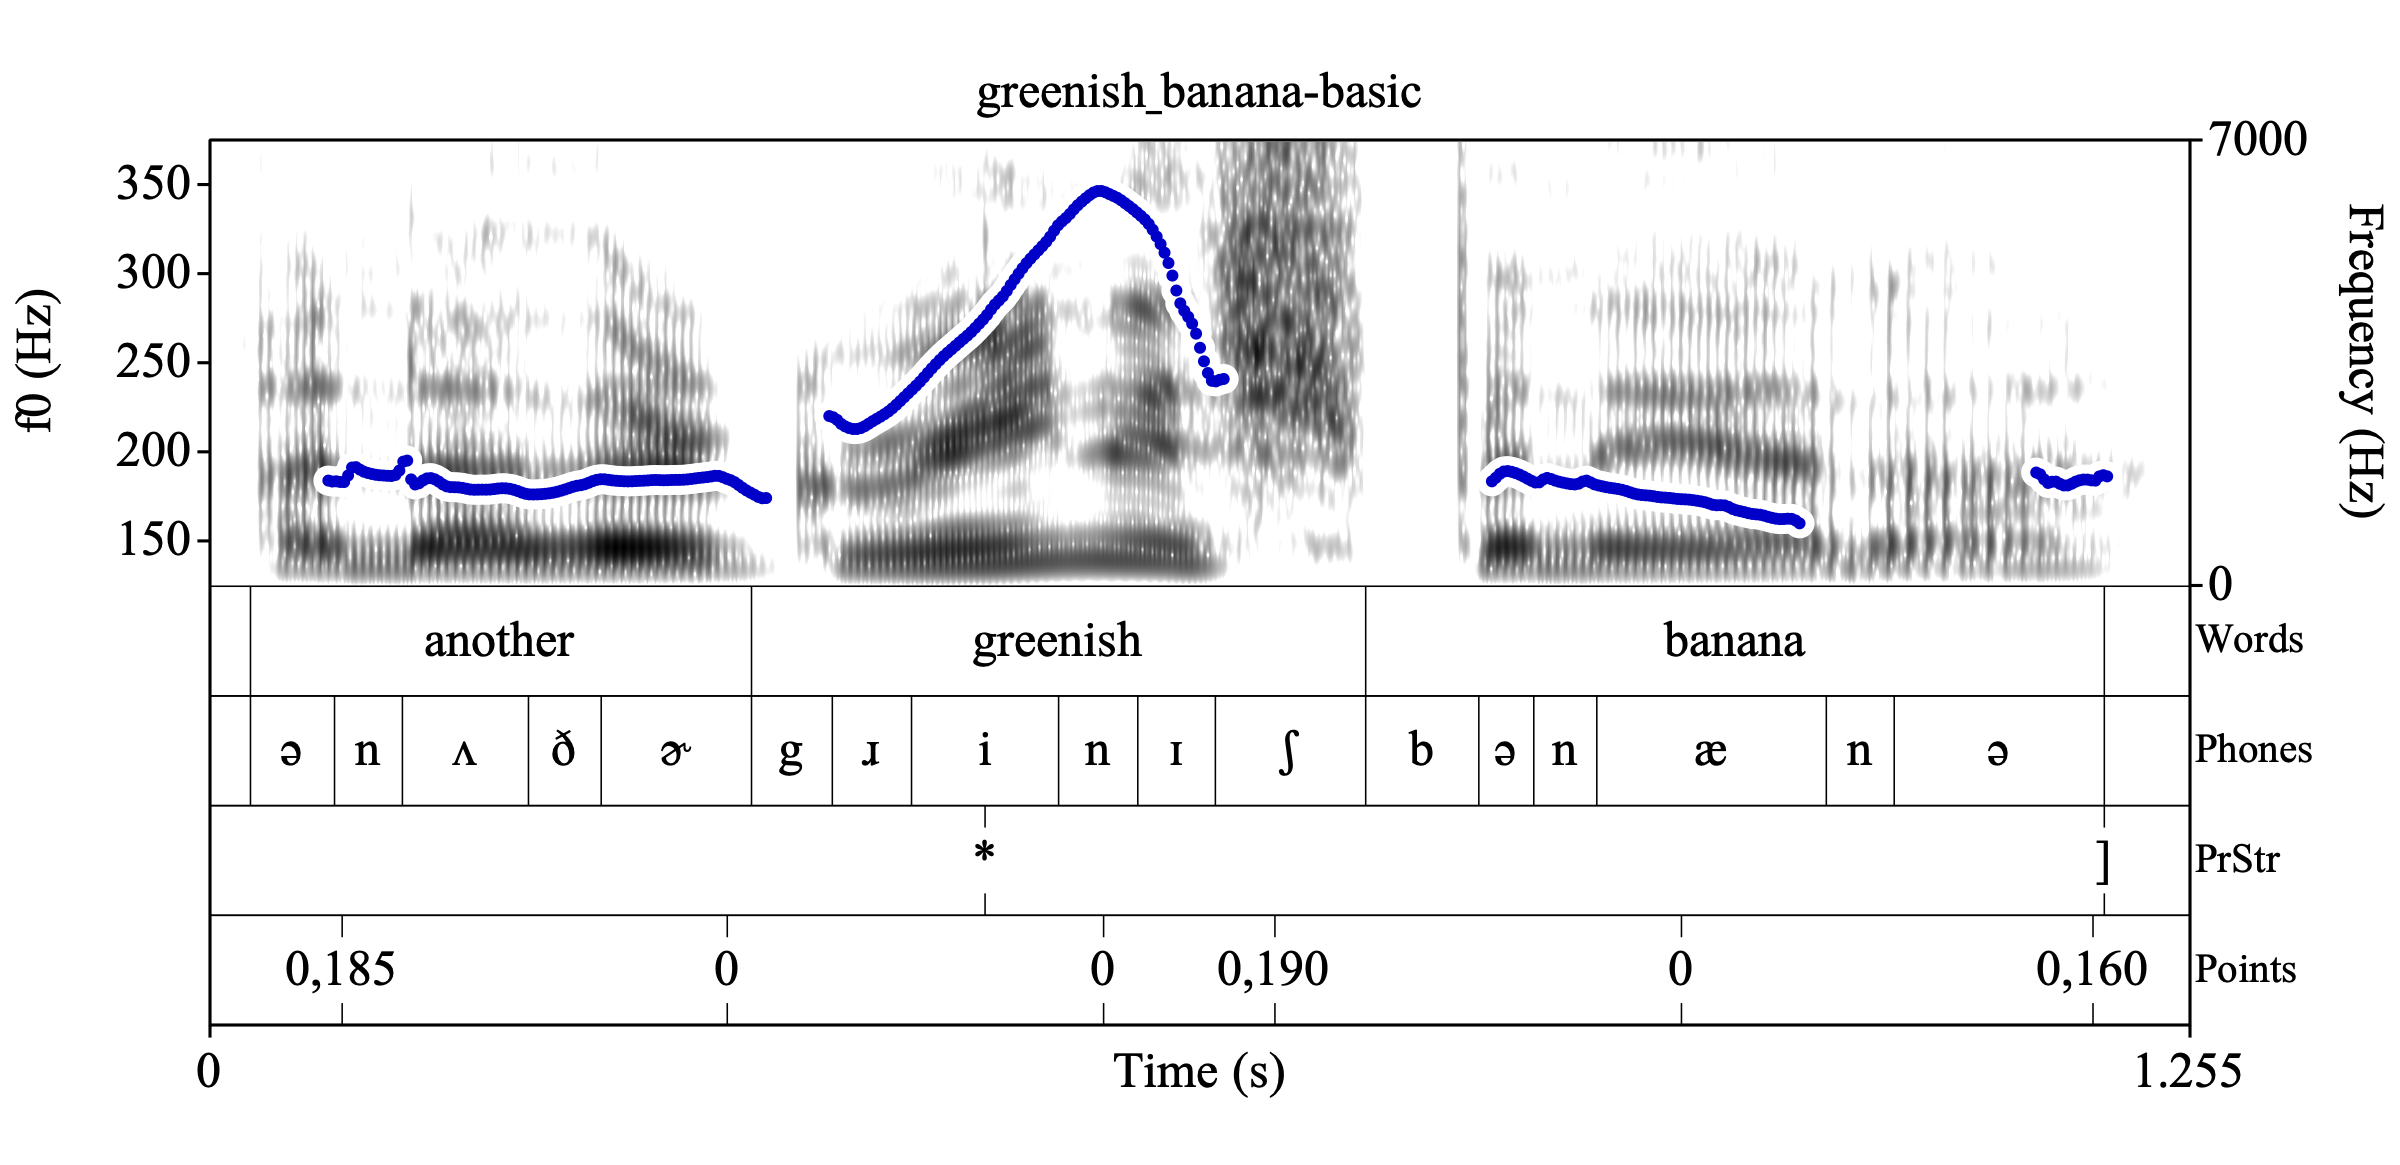
\includegraphics[width=.875\linewidth]{Points-greenish_banana-basic-comma.png}
%
\caption{\texttt{greenish\_banana}, with the f0 override PoLaR labels.%
\label{fig:greenish banana Points comma}%
\index{Annotated example, PrStr tier (basic)!greenish\_banana}%
}
\end{figure}

Let’s begin in the word “\langtext{greenish}”. Here the listener perceives a turning point in the middle of the voiceless [ʃ], and estimate its pitch value to be about 190Hz, given the slopes of the f0 track line segments that flank it. Additionally, the pitch is perceived to continuously fall during “\langtext{banana}”, so the final upward-inflected pitch at the end is perceived to be mis-tracked, and the labellers provide an inferred pitch value of 160Hz. Finally, the beginning of this utterance has an f0 at around 185Hz: the pitch tracking is a little jittery, so the labeller has appended the initial ‘\textlabel{0}’ label with ‘\textlabel{,185}’ so as to not have to worry about the software identifying an incorrect value for this turning point. Also note, again, the comma override is used to capture the final f0 in the utterance.

\paragraph{Pitch Override Points Example 4: Missing f0 during presumptive turning points\label{pitch-override-points-example-4}}

In this final example, we notice that the f0 tracking is interrupted during an interval of time at the end of the word \langtext{Stein’s}. A labeller can infer that an f0 peak might occur right during this interruption – visually, one could imagine that the pitch is rising to a peak that occurs where the two line segments would intersect, if they were lines instead of line segments. However, this inferred peak will require a comma override value, since Praat is not tracking any f0 during this time. The label ‘\textlabel{0,420}’ marks the inferred time-alignment and f0 value of this peak.


\begin{figure}[H]
\centering
%
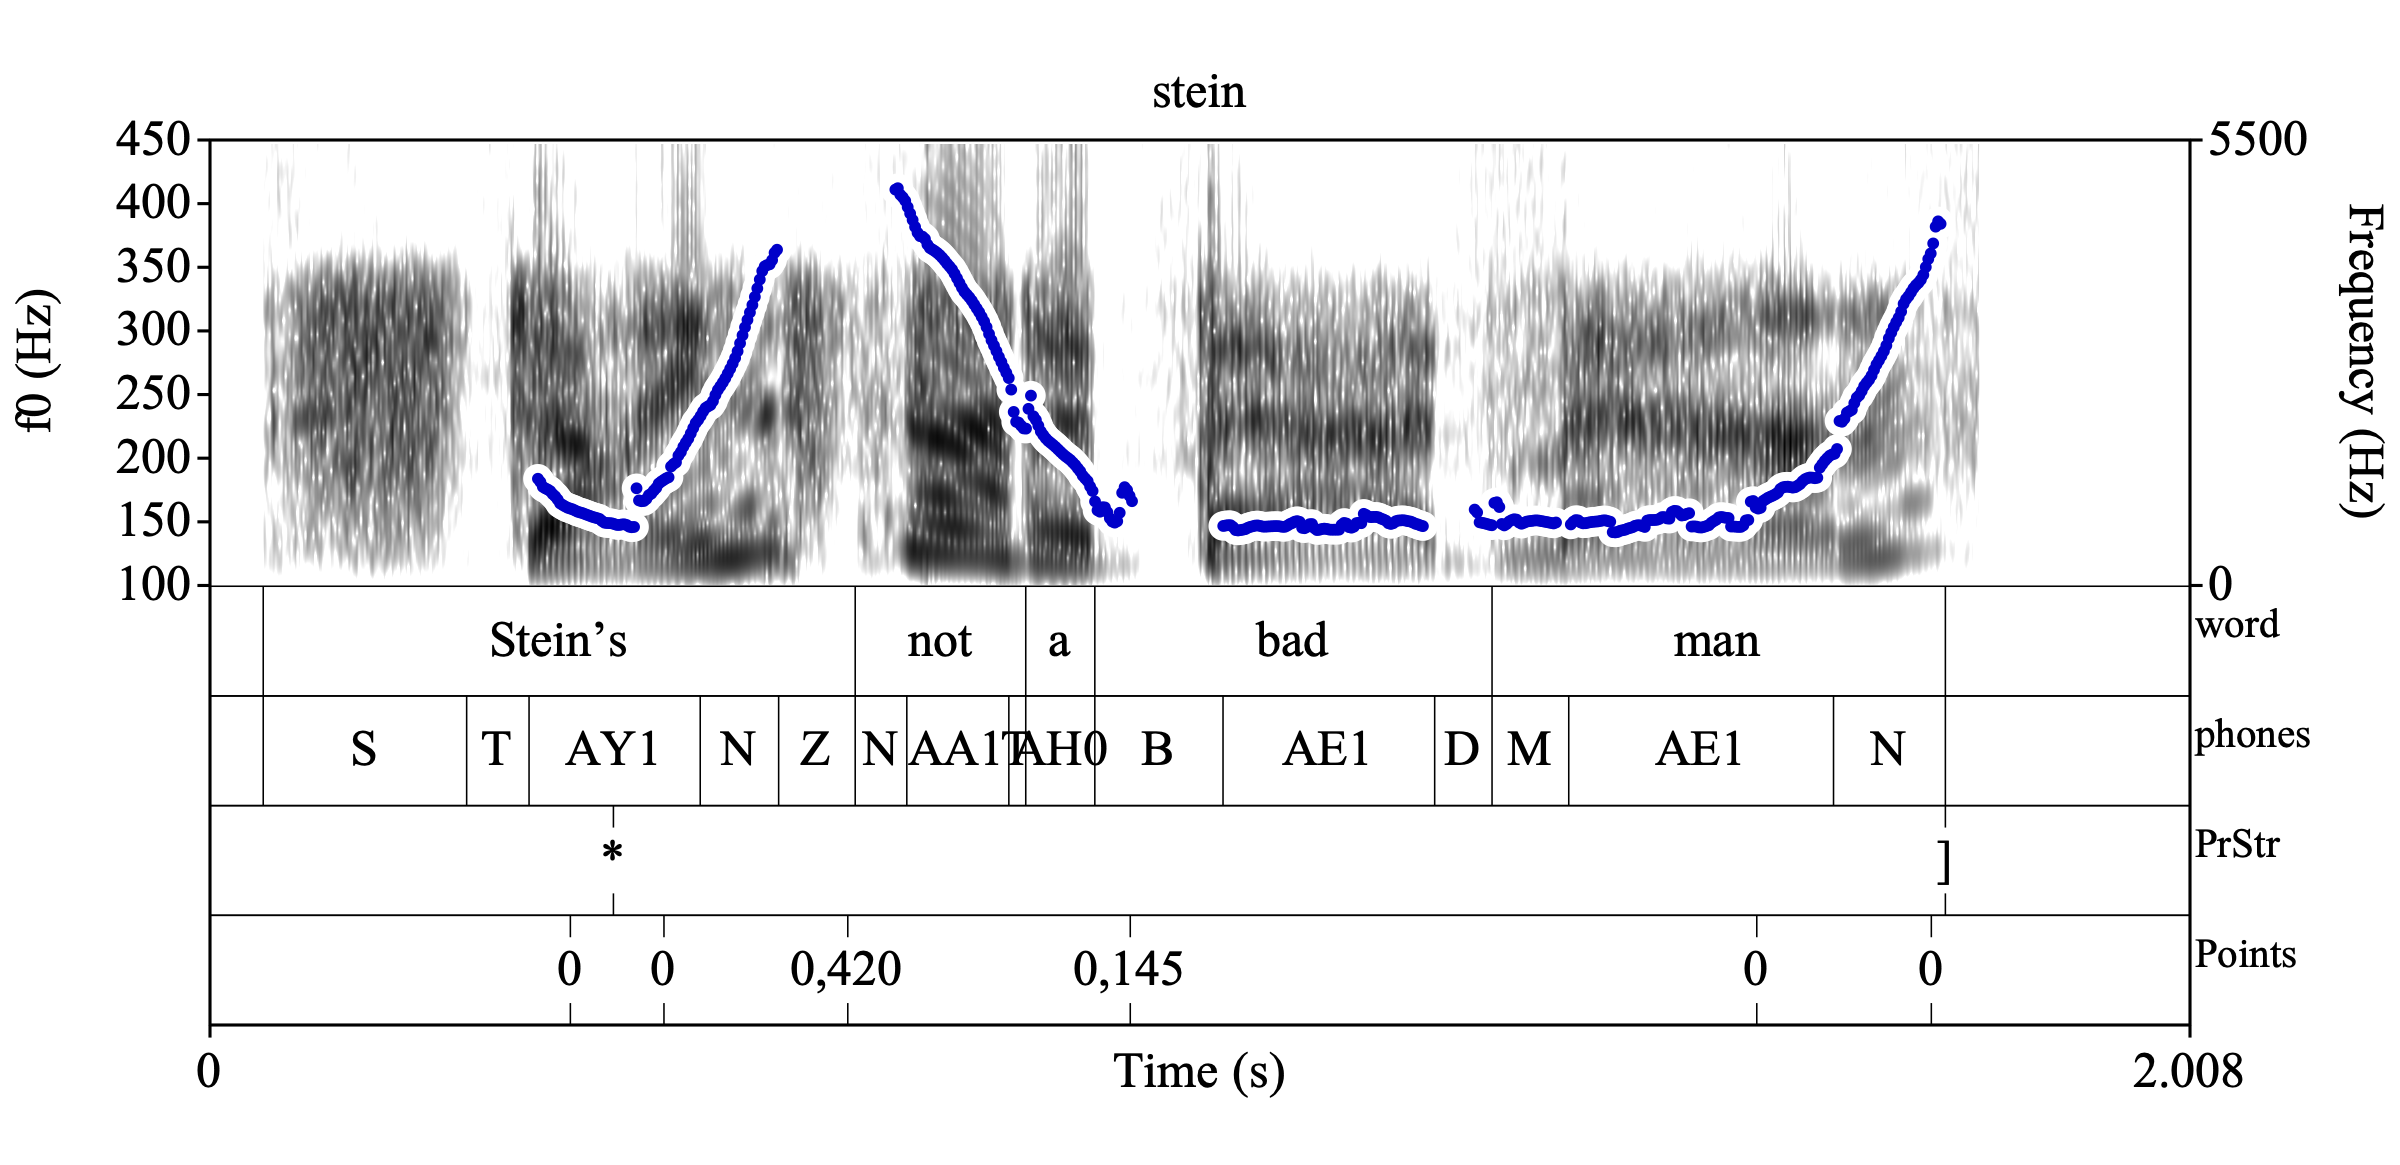
\includegraphics[width=.875\linewidth]{Points-stein-basic.png}
%
\caption{\texttt{stein}, with f0 override to label the “ghost” point at the presumptive peak.%
\label{fig:stein Points comma}%
\index{Annotated example, PrStr tier (basic)!stein}%
}
\end{figure}

The placement of the Points label (with the comma override) in the middle of this voiceless interval creates a resynthesized straight-line approximation that sounds perceptually identical, helping to justify the time-alignment and comma-override value for the ‘\textlabel{0,420}’ label.

\begin{figure}[H]
\centering
%
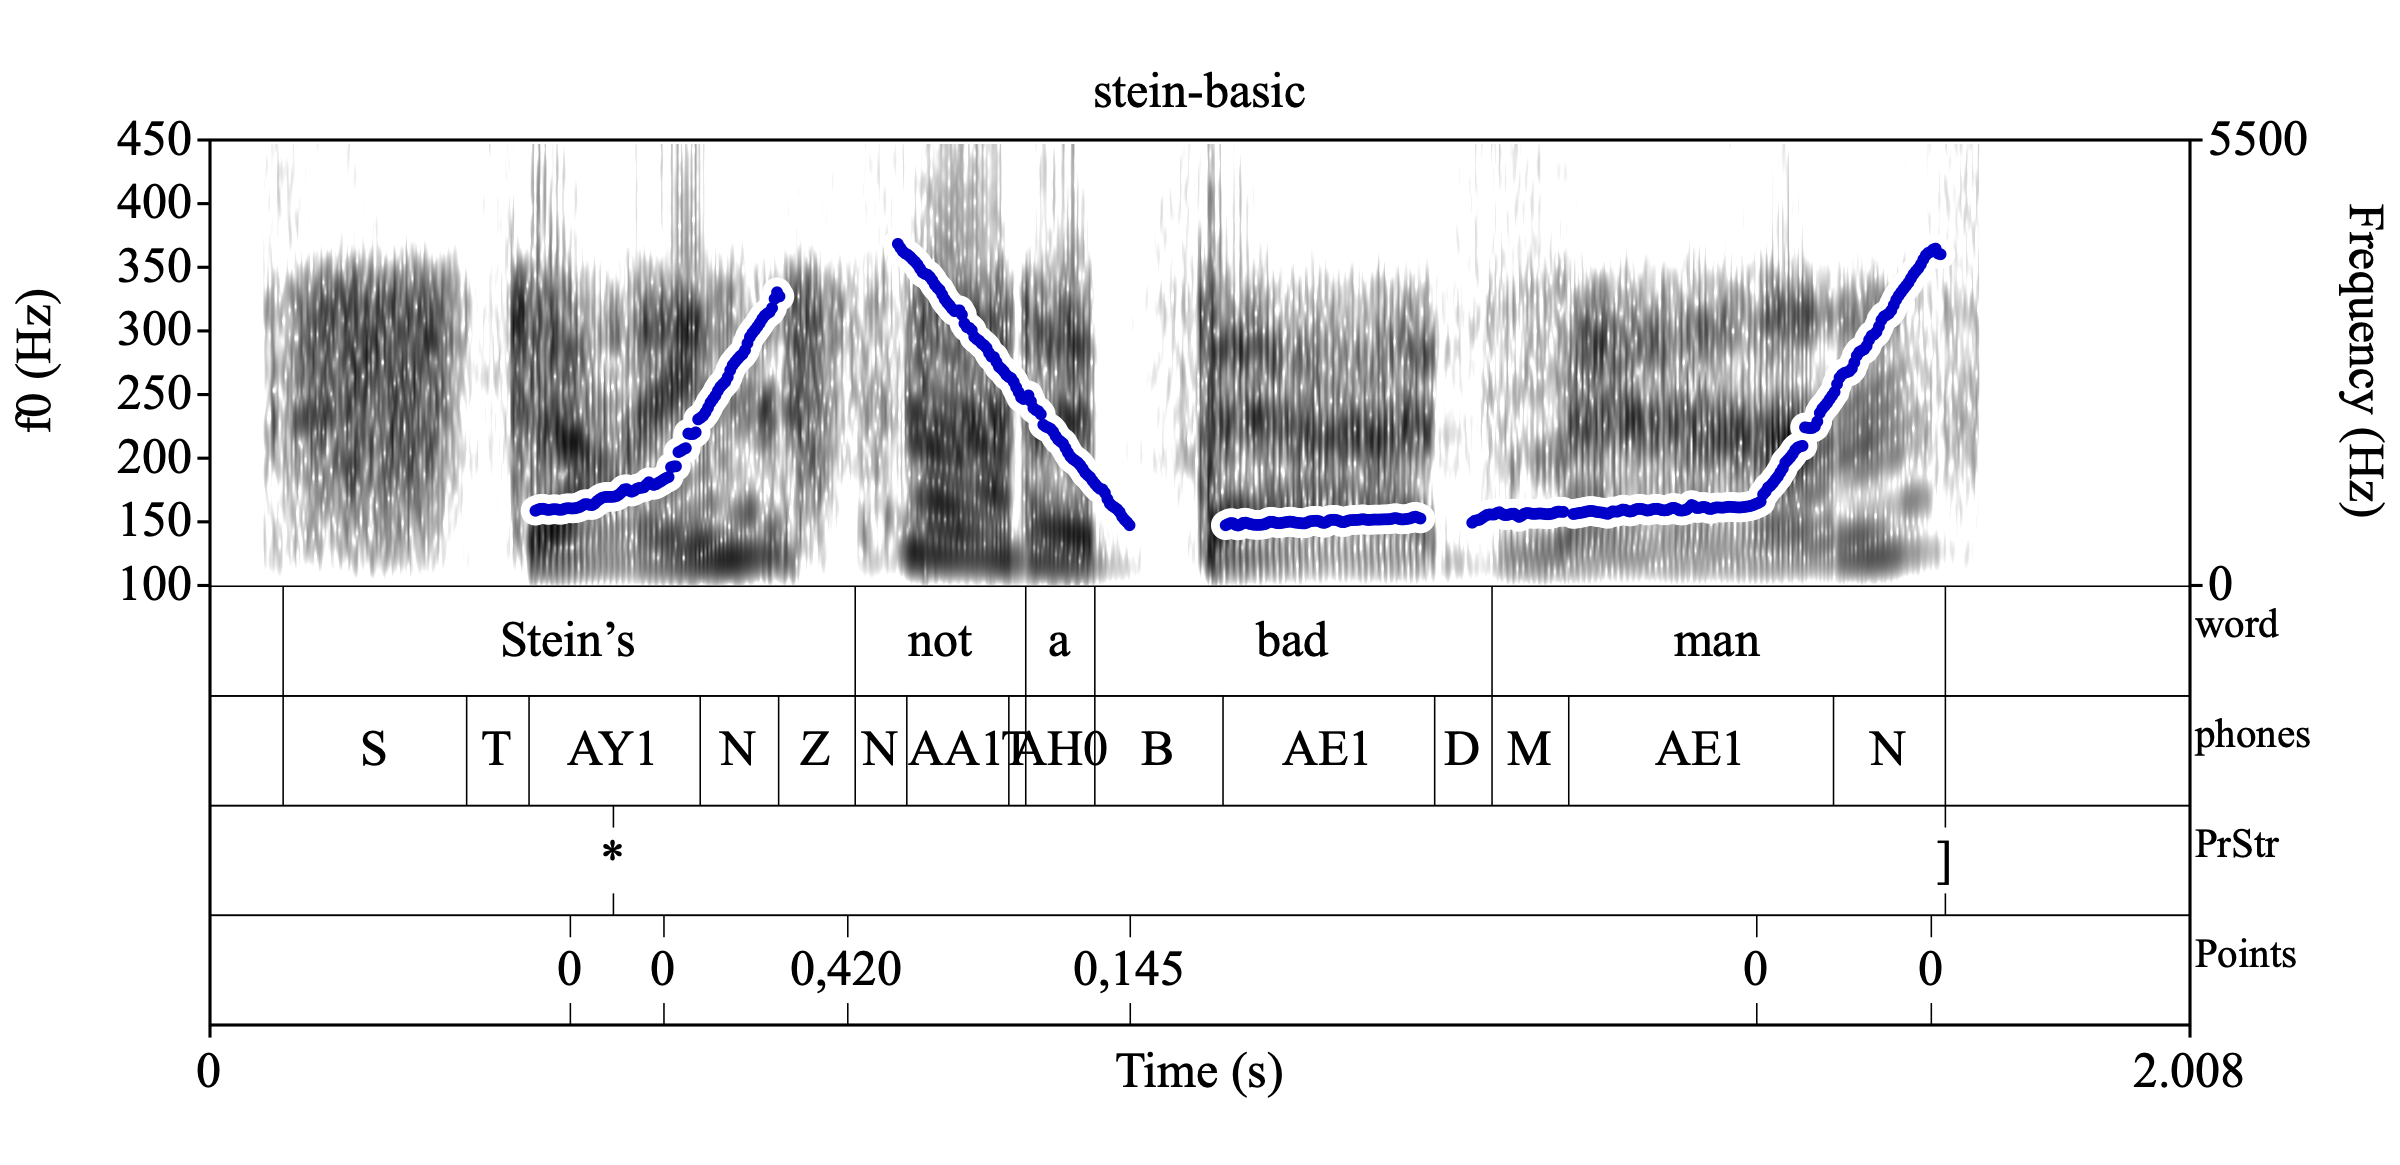
\includegraphics[width=.875\linewidth]{Points-stein-basic-resynth.png}
%
\caption{\texttt{stein}, with a straight line approximation resynthesis, on the basis of the “ghost” point peak.%
\label{fig:stein Points comma SLA}%
\index{Annotated example, PrStr tier (basic)!stein}%
}
\end{figure}


\subsubsection{Points labels summary}\label{sec:points-labels-summary}

To summarize, the three labels we have seen so far are described in Table \ref{Points basic labels}.

\begin{longtable}{cp{.8\linewidth}} \toprule \textbf{Label} & \textbf{Meaning} \tabularnewline
\midrule \endhead
\textlabel{0} & A turning point in the f0 contour (where line segments meet in a straight-line approximation of the pitch) \tabularnewline
\textlabel{?0} & Labeller is uncertain whether it is necessary to annotate a turning point in the f0 contour, even after exploring options with the straight line approximation resynthesis tool \tabularnewline
\textlabel{0,X} & An f0 turning point whose pitch value is approximately X (a labeller’s approximation of the f0 when the software-based f0 tracking is unreliable) \tabularnewline
\bottomrule 
\caption{The Basic labels for the Points tier (for English).%
\label{Points basic labels}%
}
\end{longtable}


\subsection{Ranges Tier}\label{sec:ranges}
%My first and main issue regards the Pitch Ranges tier. To summarize, a) on the x-axis (temporal dimension), labellers identify the scope of such a pitch range for different portions of an utterance. Importantly, the scope of a given pitch range is independent of phrase breaks and may be assigned to any part of an utterance. Also, b) on the y-axis, annotators identify the f0 range (min / max) of a portion of an utterance and label the min and max on a tier. Min and max do not necessary refer to the actual minimum and maximum f0 value observed in the signal, but are values that the labellers determine as minimum and maximum for a particular speaker [BTA: or context!].
% Regarding a), allowing misaligned f0 ranges and phrases is difficult both from a theoretical and practical point of view and – in my opinion – not sufficiently motivated in the manuscript. From a theoretical point of view, I am not convinced how – within one and the same phrase – speakers may employ different ranges. The authors themselves argue that phrase breaks may trigger a change in the f0 range (p. 106); I am not sure which kind of processes would trigger a change in f0 range within one and the same word. From a methodological perspective, this assumption or possibility in PoLaR might lead to inconsistencies in labelling. That is, I am concerned about both the validity of the range annotation and its reliability. In fact, even though I am quite experienced in annotation, I would not have placed all f0 ranges as done by the authors, e.g., on p. 46, 106, 108, 109. I thus wonder how reliable the positioning of these range spaces is, which in turn, has implications for the pitch levels, as they are informed by the pitch ranges.
	%> response: address this by raising the question of "what are Ranges supposed to do?" and then describe how there are researcher-/project-level choices that can be made to further guide choices
	%> labellers are encouraged to *consider* whether there is a new Ranges interval, according to…
		%> phrase boundary (new phrase <-/-> new Range, but the two do have high co-incidence)
		%> downstep / upstep (phonologically conditioned changes)
			%> this can occur word-medially!
		%> voice quality shifts (modal -> falsetto; extended creak -> modal)
%With respect to b) (y-axis), I also have a methodological and a theoretical concern: Methodologically, I think that inferring speakers’ actual highs and lows requires intensive experience and such inferences are particularly prone for interrater variability. More importantly, assigning pitch levels based on the min/max of the f0 range represents a normalization that gets rid of the actual f0 values – which in some cases might be relevant indeed. I totally see that in some cases, e.g., the cases of range compression (p. 104) it is straightforward to apply such a normalization, but there might be cases, e.g., in different registers such as infant-directed speech, in which information of the actual values of pitch targets is important (e.g., when voices go into falsetto). Taken together, the Ranges Tier in my view allows for too many “degrees of freedom” (Roettger, 2019) for labellers. This, in turn, may decrease reproducibility and reliability, which brings me to my second point.
	%> response: there is variation, of course, but again – what matters is what the researcher **aims to do** with them. anecdotally, we have found that there are differences, of course, in labels here but they are *surprisingly* more consistent than might be expected
	%> response: again, this is a question of what we ought to do with Ranges annotations.
		% should we compare annotations across labs? only with care!
		% should we be able to compare ranges within labs? ABSOLUTELY!
		% does this f0 normalization (ranges->levels) erase variation? kind of, but on purpose, and in a way that actually allows labellers to keep track of the shifts (e.g., going into falsetto is tracked by Ranges in a way that is completely untracked in other annotation systems)
The Range Domains Tier is an interval tier, in which the pitch range is annotated over a portion of speech. In essence, a shift in “Range” is a shift in what counts as low and/or high pitch.

Accordingly, the key function of the Ranges tier is to define the local lows and highs that intonation alternates between: changing ranges allows you to compare two different pitch values and say they’re both "highs" even if one is much higher\slash lower than the other. Before we discuss how this tier is labelled, some pre-discussion is necessary about “pitch range”.

We assume that there are three usages of the term “pitch range”.\footnote{For a more in depth discussion and overview of pitch range, as well as the related terms “pitch span” and “pitch register,” see \citealt{gussenhoven04}, Chapter 5, especially pp. 77-80.} These three usages are: (i) the “physiological pitch range” of the speaker, covering frequencies from all the pitches that their vocal anatomy allows them to produce, (ii) the “comfortably implementable pitch range” of the speaker, covering a speaker’s comfortable low pitch to their comfortable high pitch, and (iii) the “local pitch range” within a particular utterance, which operationally demarcates where “low” targets and “high” targets go, for this particular portion of speech.

For example, consider the following example from NPR radio (\href{https://www.npr.org/sections/goatsandsoda/2018/05/11/603315432/the-best-mothers-day-gift-get-mom-out-of-the-box}{source}):

\begin{figure}[H]
\centering
%
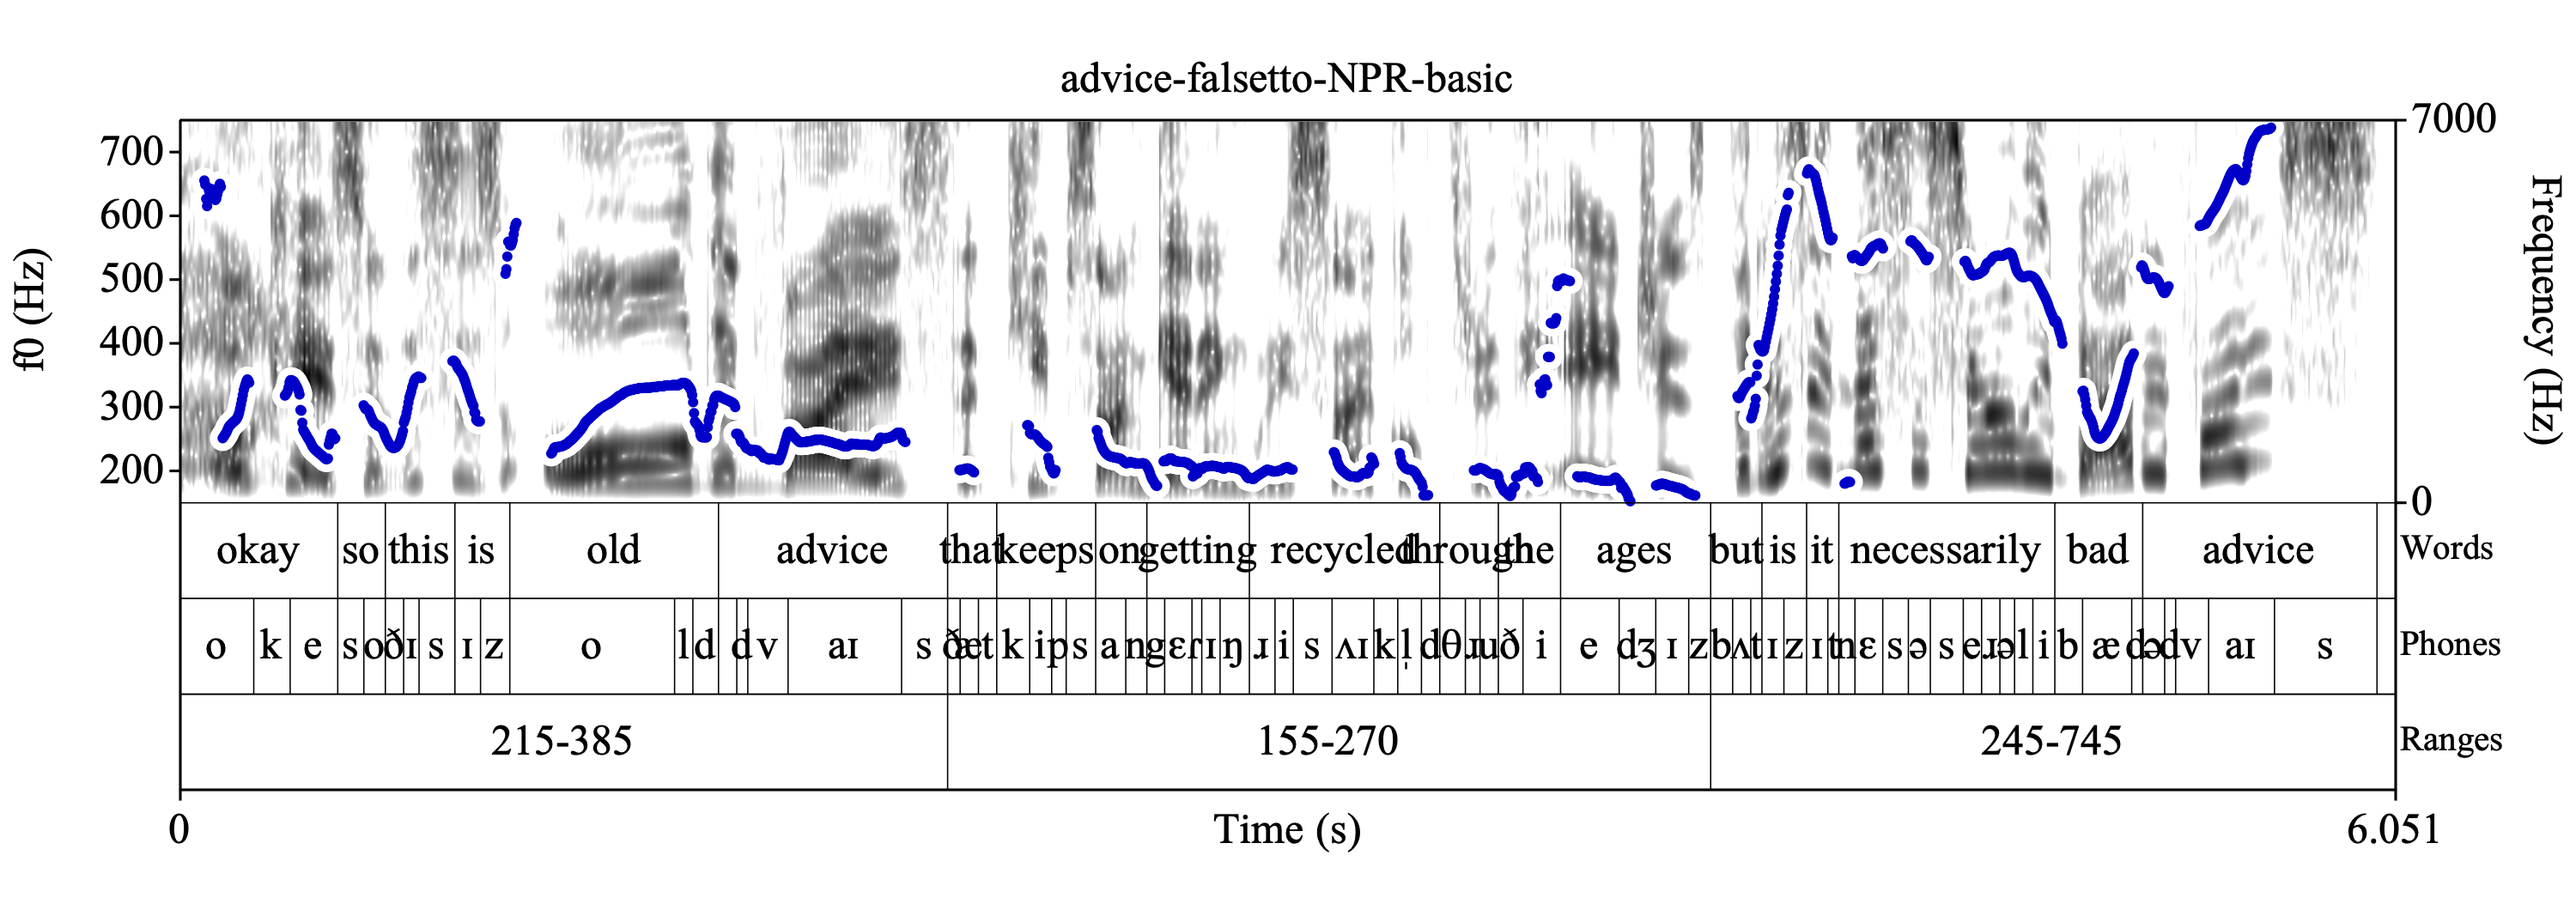
\includegraphics[width=\linewidth]{Ranges-advice-falsetto-basic-all-3-ranges.png}
%
\caption{An example of a long utterance with three pitch range intervals.%
\label{fig:advice-falsetto Ranges basic}%
\index{Annotated example, Ranges tier (basic)!advice-falsetto}%
}
\end{figure}

Let us discuss how this example embodies all three types of pitch ranges. Here, the speaker must have a \uline{physiological pitch range} that allows at least a range of 150Hz-750Hz (though likely it is bigger). In the latter part of the recording, the speaker is using a falsetto voice, and the end of the utterance could be analyzed as “super high” in that high falsetto range. Depending on the speaker, this extreme falsetto high pitch can reasonably be considered outside of their \uline{comfortably implementable pitch range}.

Viewing the entire utterance as a whole, one can perceive it as having three different \uline{local pitch ranges}, \textbf{each of which is labelled as an interval on the “Ranges” tier}. Consider the high and low pitch in “\langtext{okay so this is old advice}” compared to the highs and lows in “\langtext{but is it necessarily bad advice}”. Although the highs and lows in “\langtext{okay\ldots advice}” are much lower than in “\langtext{but is it\ldots advice}”, on their own, they can be perceived as \uline{locally} high (even though, e.g., “\langtext{okay}” is much lower than the later highs) and low. Similarly, these highs and lows are also different from the highs and lows in “\langtext{that keeps on getting recycled through the ages}”.

Labelled Range boundaries do not always co-occur with prosodic phrase boundaries. A local pitch range interval may span multiple prosodic phrases. An example of this can be found for an early part of the advice-falsetto-NPR example:

\begin{figure}[H]
\centering
%
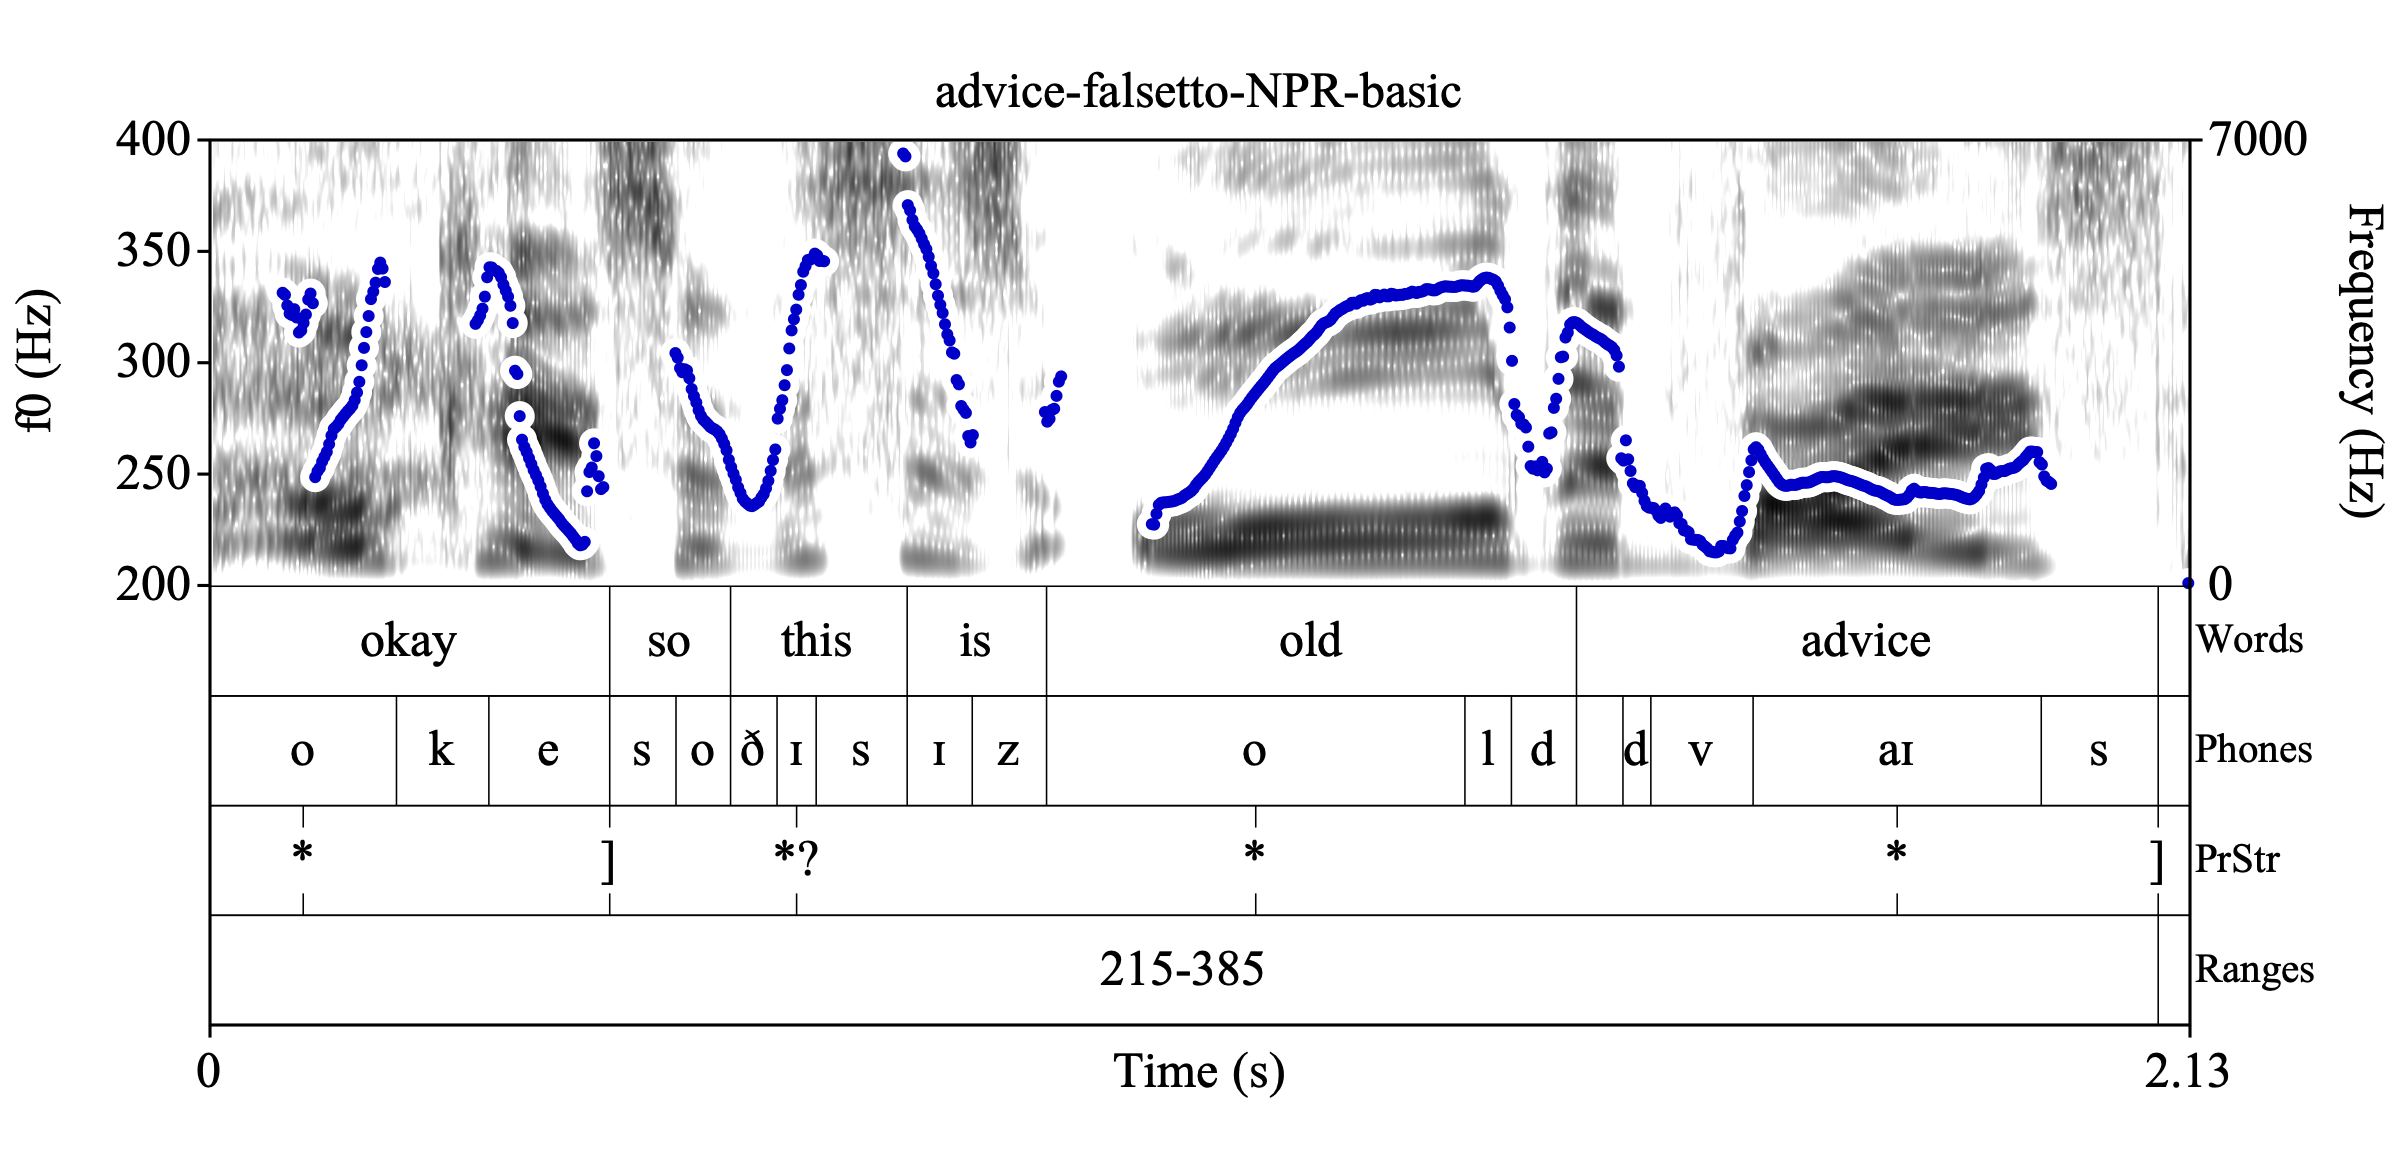
\includegraphics[width=.875\linewidth]{Ranges-advice-falsetto-basic-first-range.png}
%
\caption{Two prosodic phrases (PrStr annotation) and one local pitch range (Ranges annotation).%
\label{fig:advice-falsetto PrStr Ranges basic}%
\index{Annotated example, Ranges tier (basic)!advice-falsetto}%
\index{Annotated example, PrStr tier (basic)!advice-falsetto}%
}
\end{figure}

Conversely, a single phrase as labelled in the PrStr tier may contain multiple ranges, a topic which will be addressed in more detail in section \ref{sec:ranges-advanced} of chapter \ref{ch:advanced}.

Because Ranges constituents need not have a one-to-one correspondence to prosodic phrases on the PrStr tier, the Ranges tier labeller need not even have PrStr tier labels to do their work, and the Ranges tier can be labelled independently of all other tiers. If the PrStr tier is in place, when a new prosodic phrase begins, it’s not necessarily the case that there will be a new local pitch range. At the same time, it seems that in some cases a new local pitch range may serve as a cue that a new prosodic phrase has begun (cf. \citealt{brugos15}, \citealt{brugos-18}, and \citealt{kim20}). In this way, a labeller may find it useful to consider whether a new range interval is necessary when there is a new phrase, but they do not necessarily need to attend to conventional prosodic phrase boundaries when doing this labelling.

Labelling the Ranges tier requires labellers to consciously engage in thinking about concepts that may be unfamiliar (e.g., identifying locally “high” pitch, even where the speaker is speaking in a low and narrow pitch range). Not many individuals are practiced in engaging their intuition in this way, and new labellers may find it challenging. Ultimately, however, these intuitions will be necessary for relating the Points tier to more categorical labels of pitch “height” (e.g., values 1-5 on the Levels tier, or “high”\slash ”low” even more generally). More on this will be addressed in section \ref{sec:ranges-advanced} of chapter \ref{ch:advanced}.

\subsubsection{Getting started with the annotation of Ranges:}\label{sec:getting-started-with-the-annotation-of-ranges}

Each stretch of PoLaR-labelled speech must contain minimally one pitch range, i.e., an f0 floor and an f0 ceiling must be noted for that stretch of speech, such that the f0 minimum and maximum for that stretch are captured within that range. As a rule of thumb when starting out labelling, the labeller may find it useful to consider the pitch range to every speech interval bounded by strong temporal cues to phrase boundaries, such as silent pauses or breaths. (Bear in mind that such a group may well contain more than one range, and or that sequential stretches of speech separated by a pause or other boundary cues may be contained within a single range.)

If the labeller has access to PrStr labels, they may find it useful to consider ranges with respect to phrases as delimited by the \textlabel{]} label. At the same time, domains for ranges need not be determined by phrases labelled in the PrStr tier. Even a short stretch of speech may well turn out to contain local pitch range changes, as described in the Advanced labels chapter (Ch.\ref{ch:advanced}). Conversely, sequential phrases may be perceived as part of the same range. Ranges may to some extent suggest groupings among phrases, such as those labelled with \textlabel{]} in the PrStr tier. In this way, PoLaR Ranges annotation gives the labeller the means to capture more complicated relations where phrase boundaries (as annotated via the PrStr tier) and ranges can be somewhat independent: ranges can be annotated delinked from other boundary cues.

\subsubsection{Local Pitch Ranges: Typical Cases}\label{sec:local-pitch-ranges-typical-cases}

The most straightforward case will be an isolated short phrase, with a small number of events labelled in the Points and PrStr tiers, and a single labelled pitch Range. However, in dynamic speech, utterances of more than a few words are likely to consist of more than one range interval.

For each (part of an) utterance, a speaker (often unconsciously) picks out a portion of their physiological pitch range, the lower part of which corresponds to frequencies for their (locally defined) lows, and the higher part of which corresponds to frequencies for their (locally defined) highs. In an ideal case, the intonational contour for an utterance will produce measurable f0 such that the minimum f0 is at (or around) the minimum of the local pitch range, and the maximum f0 is at (or around) the maximum of the local pitch range. Thus, if the f0 tracking (modulo any tracking errors) identifies the lowest f0 in an interval of time as 112.4Hz and the highest f0 in that same interval as 273.2Hz, the labeller can assume that these measurements reflect the local pitch range that the speaker is employing.

At the same time, the labeller should be a little cautious, and give a little wiggle room from the measured f0 min\slash max (rounding up or down to a number ending in 5 or 0, typically by at least 1 or 2 Hz, and often by a few more), since precise numbers are influenced by a number of factors, including software settings. Thus, a measured f0 range of 112.4Hz to 273.2Hz should have the min rounded down and max rounded up, and then be annotated as an interval in the Ranges tier with a label like ‘\textlabel{110-280}’. In other words, \textbf{in the typical case, (rounded) measures of local f0 min and local f0 max can be used to determine the label for a Ranges interval}. (This is the default guidance; more complex cases will be discussed here and in section \ref{sec:ranges-advanced} of Ch.\ref{ch:advanced}.)

Figure \ref{fig:amelia-knew2 Ranges basic} shows an example of a file annotated with the Ranges tier. Here, the minimum f0 is 114.7 Hz (in the [u] of “\langtext{minimum}”), and the maximum f0 is 248.3 Hz in the [l] of Amelia. The labeller has rounded down to a range minimum of 110 Hz and rounded up to a range maximum of 250 Hz.

\begin{figure}[H]
\centering
%
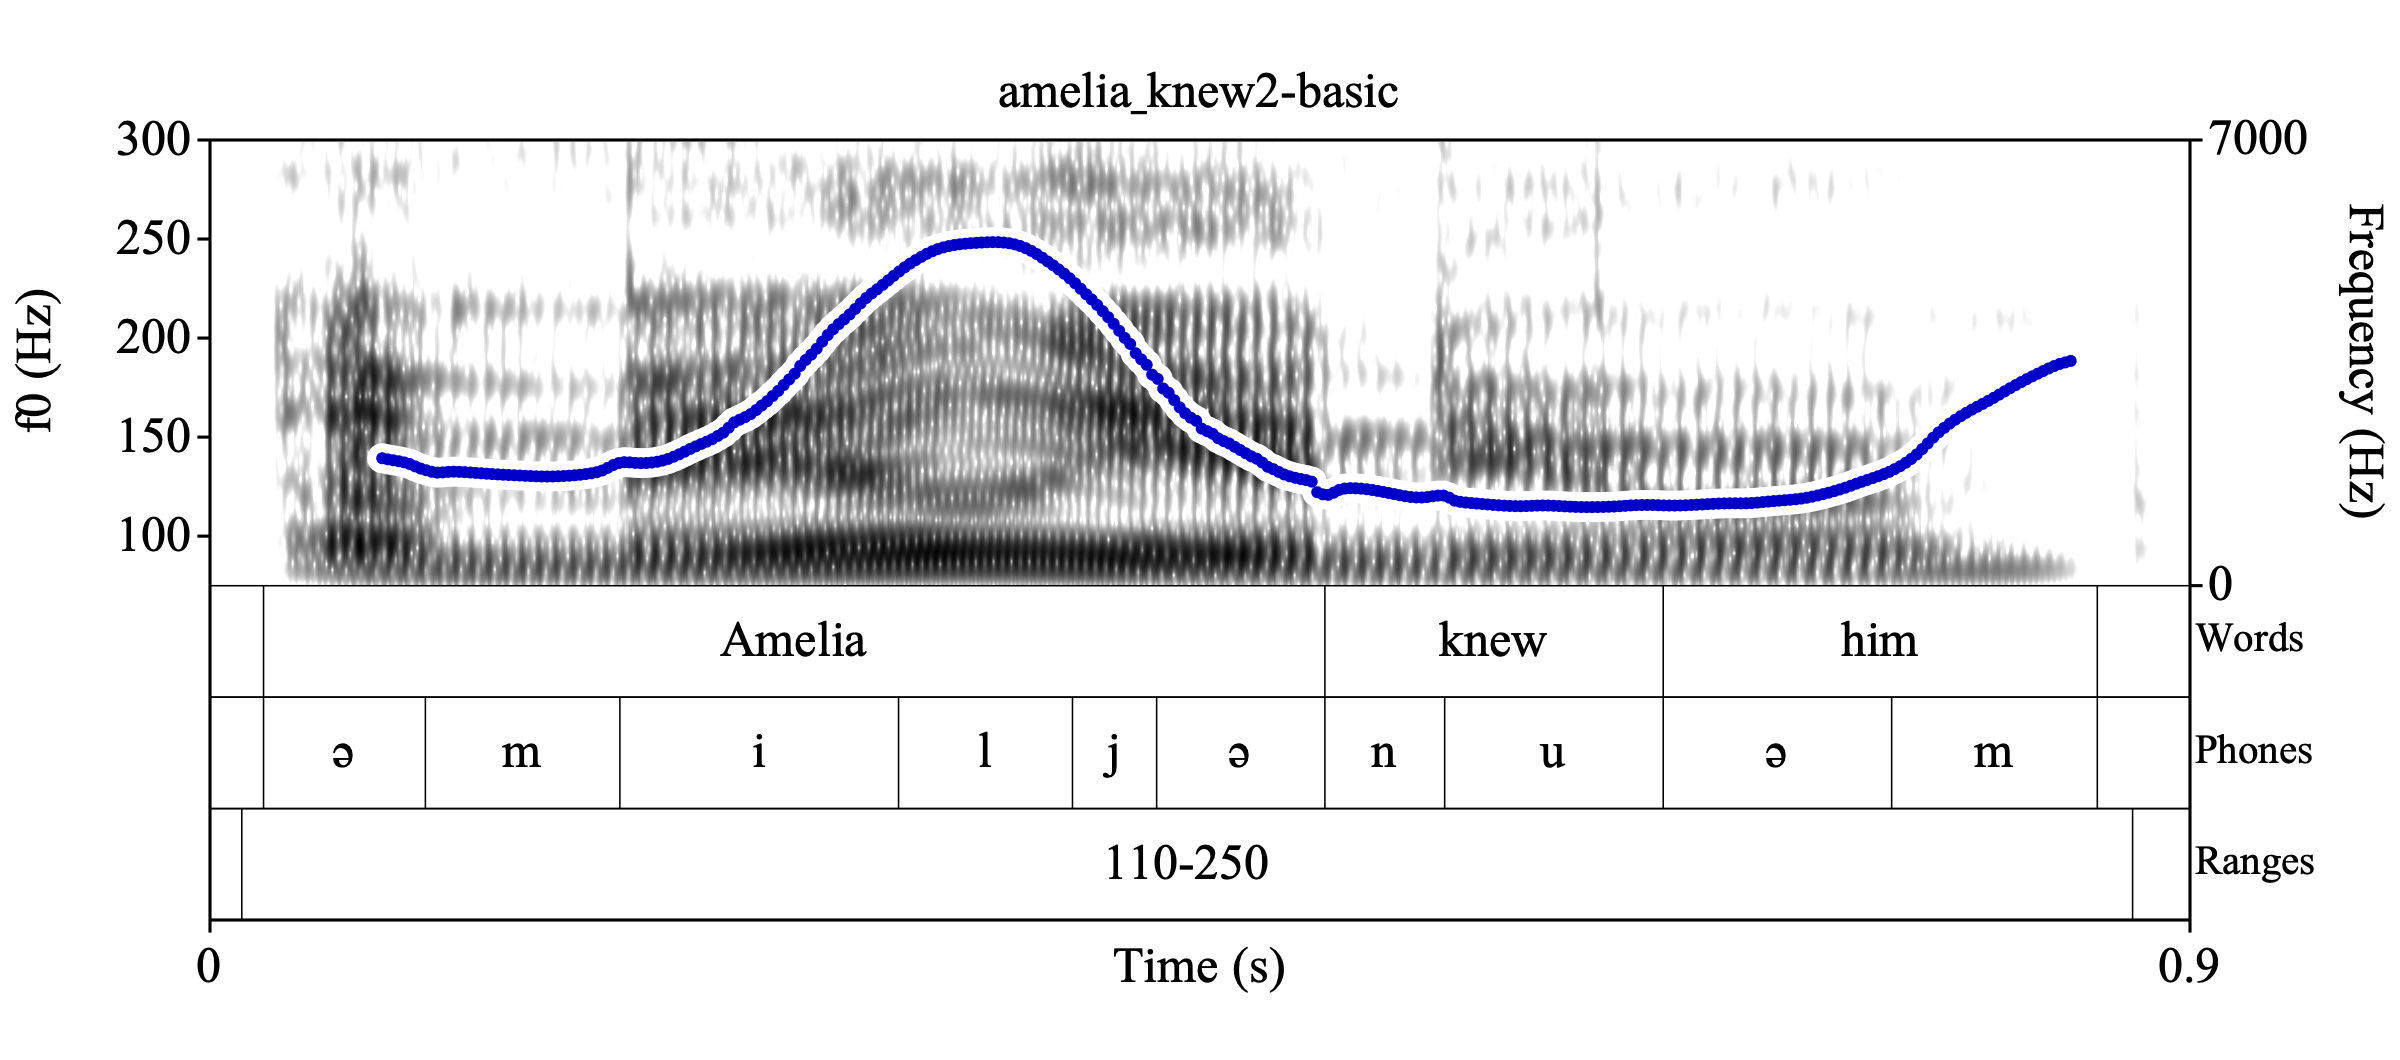
\includegraphics[width=.875\linewidth]{Ranges-amelia_knew2-basic.png}
%
\caption{An example of a short utterance with single pitch range interval, and clear pitch tracking.%
\label{fig:amelia-knew2 Ranges basic}%
\index{Annotated example, Ranges tier (basic)!amelia-knew2}%
}
\end{figure}

\begin{figure}[H]
\centering
%
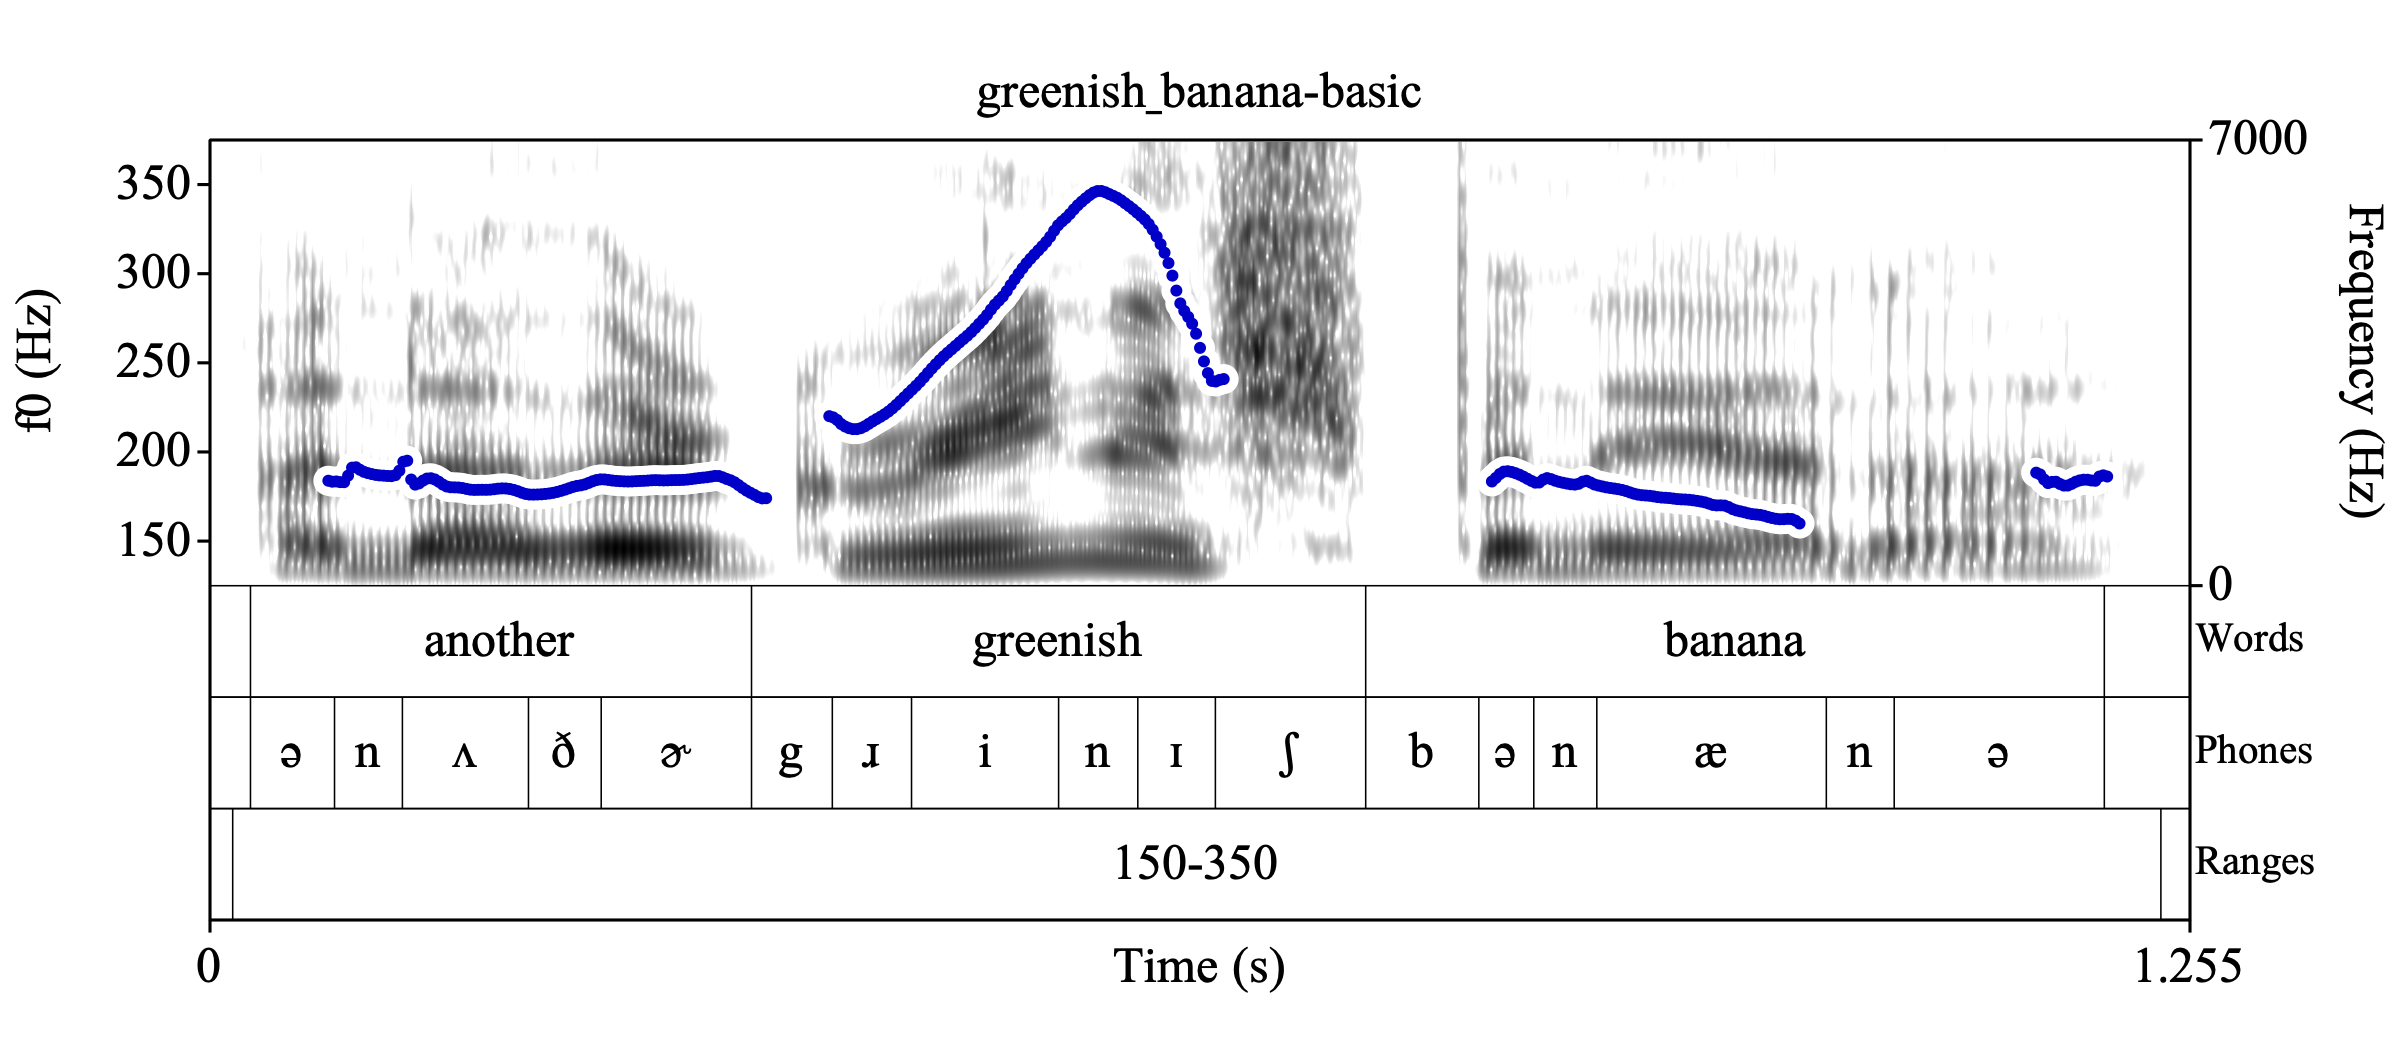
\includegraphics[width=.875\linewidth]{Ranges-greenish_banana-basic.png}
%
\caption[An example of a short utterance with single pitch range interval.]{An example of a short utterance with single pitch range interval, and a region of unreliable pitch tracking at the bottom of the speaker’s range.%
\label{fig:greenish-banana Ranges basic}%
\index{Annotated example, Ranges tier (basic)!greenish-banana}%
}
\end{figure}

Unlike in the example in Fig. \ref{fig:amelia-knew2 Ranges basic}, which shows a smooth pitch track, this example in Fig. \ref{fig:greenish-banana Ranges basic} shows pitch tracking unreliability where the speaker has produced creaky voice at the end of the utterance. In this case, the lowest reliable f0 is in the [æ] of banana, at 162 Hz. The labeller has chosen to round the bottom of the pitch range a bit lower, using 150 Hz. (The maximum of 345 Hz takes place during a region of reliable pitch tracking, and the labeller has rounded up to 350 Hz.) Pitch tracking errors at the end of phrases are very common, especially when the pitch is low and/or the speaker ends up creaking. The labeller should use their best estimate of how low the perceived f0 goes. 

The next example in Figure \ref{fig:no_cigar Ranges basic} (\texttt{no\_cigar}) shows a short utterance with two ranges, and the example following in Figure \ref{fig:tomorrow_morning Ranges basic} (\texttt{tomorrow\_morning}) shows another short utterance, this one with one range.


\begin{figure}[H]
\centering
%
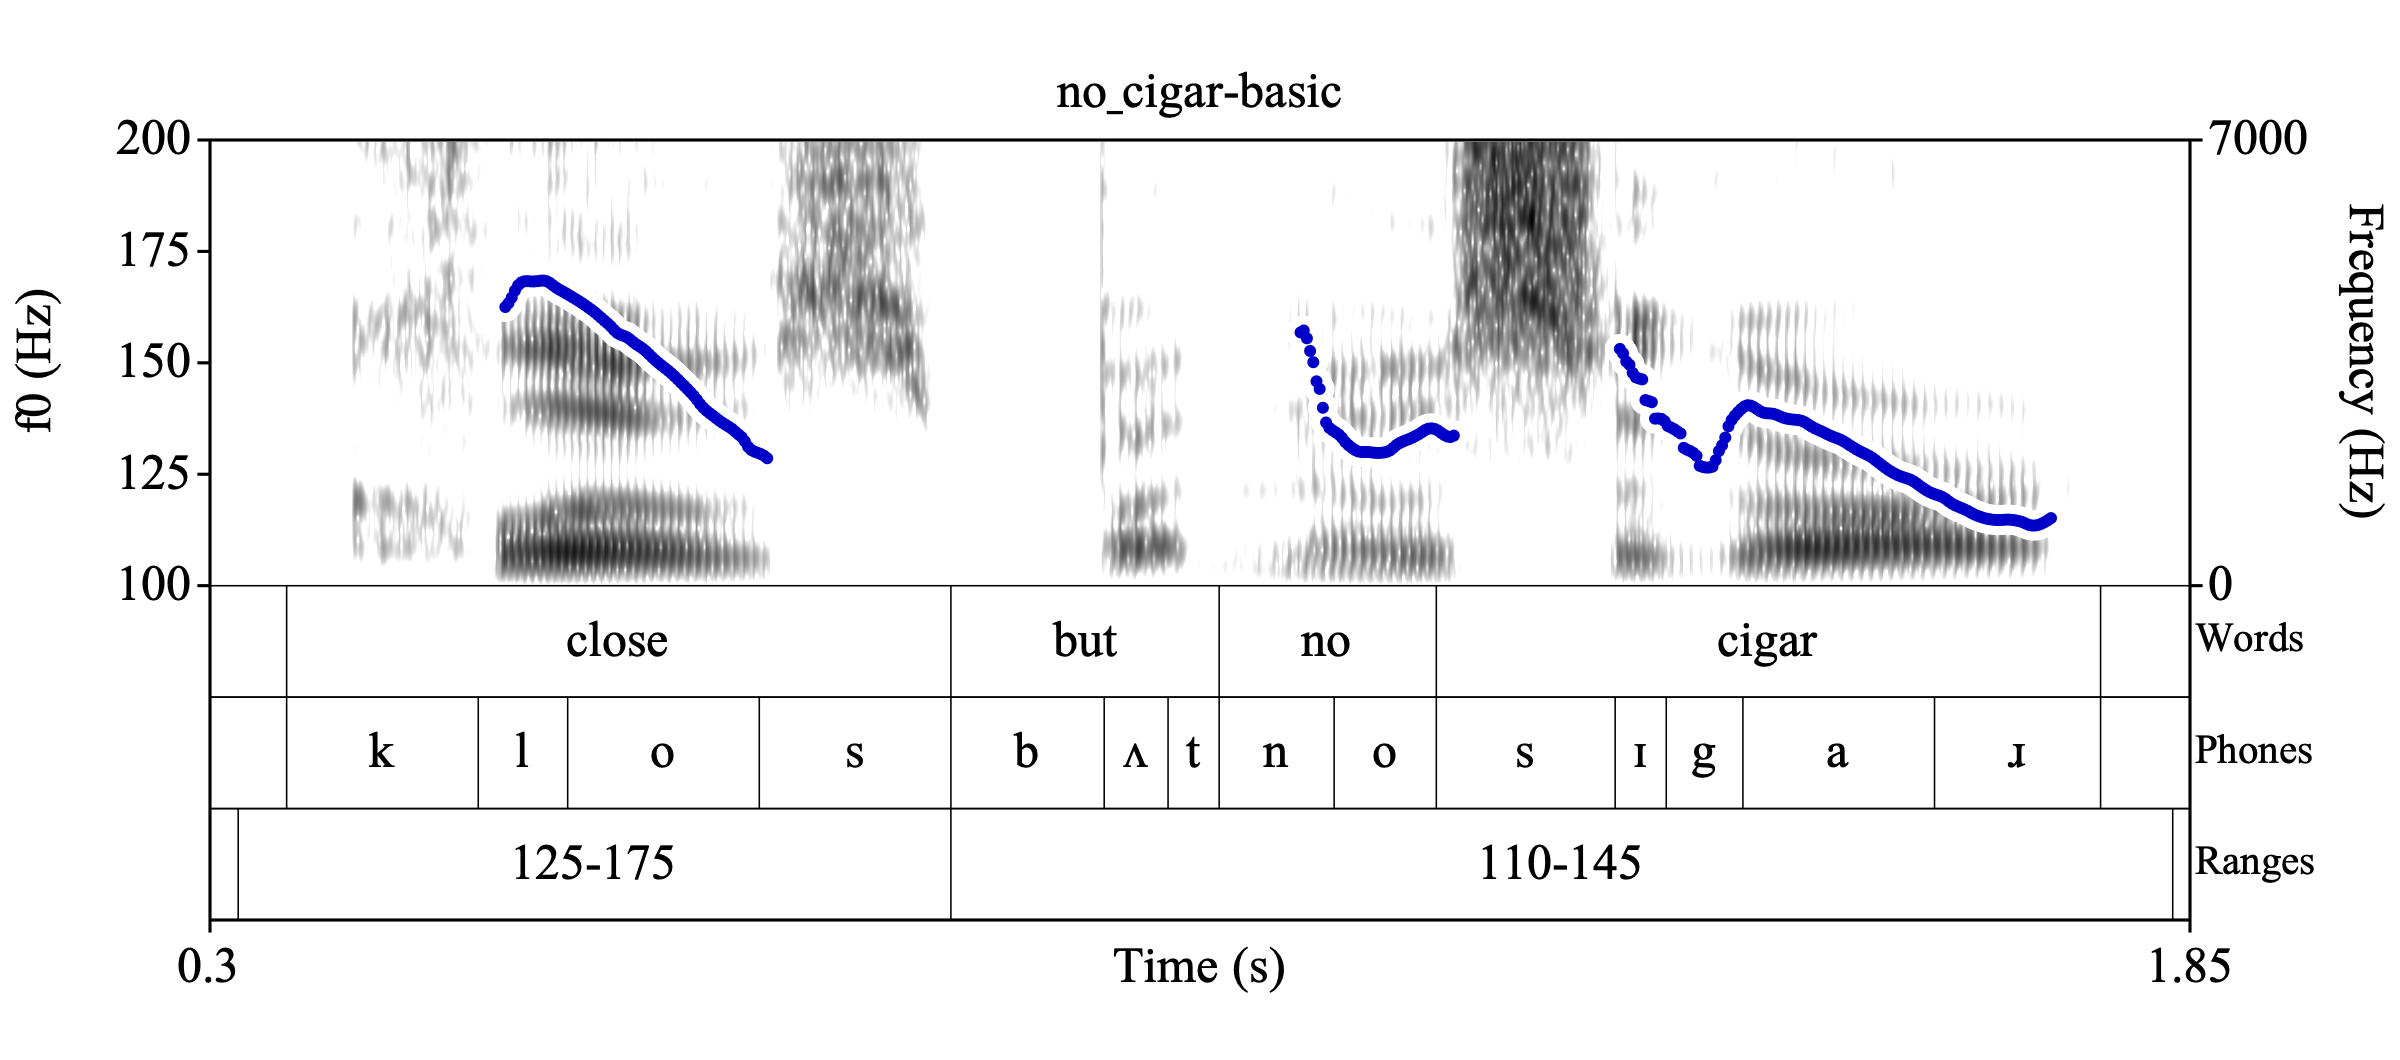
\includegraphics[width=.875\linewidth]{Ranges-no_cigar-basic.png}
%
\caption{This is an example of a short utterance with two ranges.%
\label{fig:no_cigar Ranges basic}%
\index{Annotated example, Ranges tier (basic)!no\_cigar}%
}
\end{figure}


\begin{figure}[H]
\centering
%
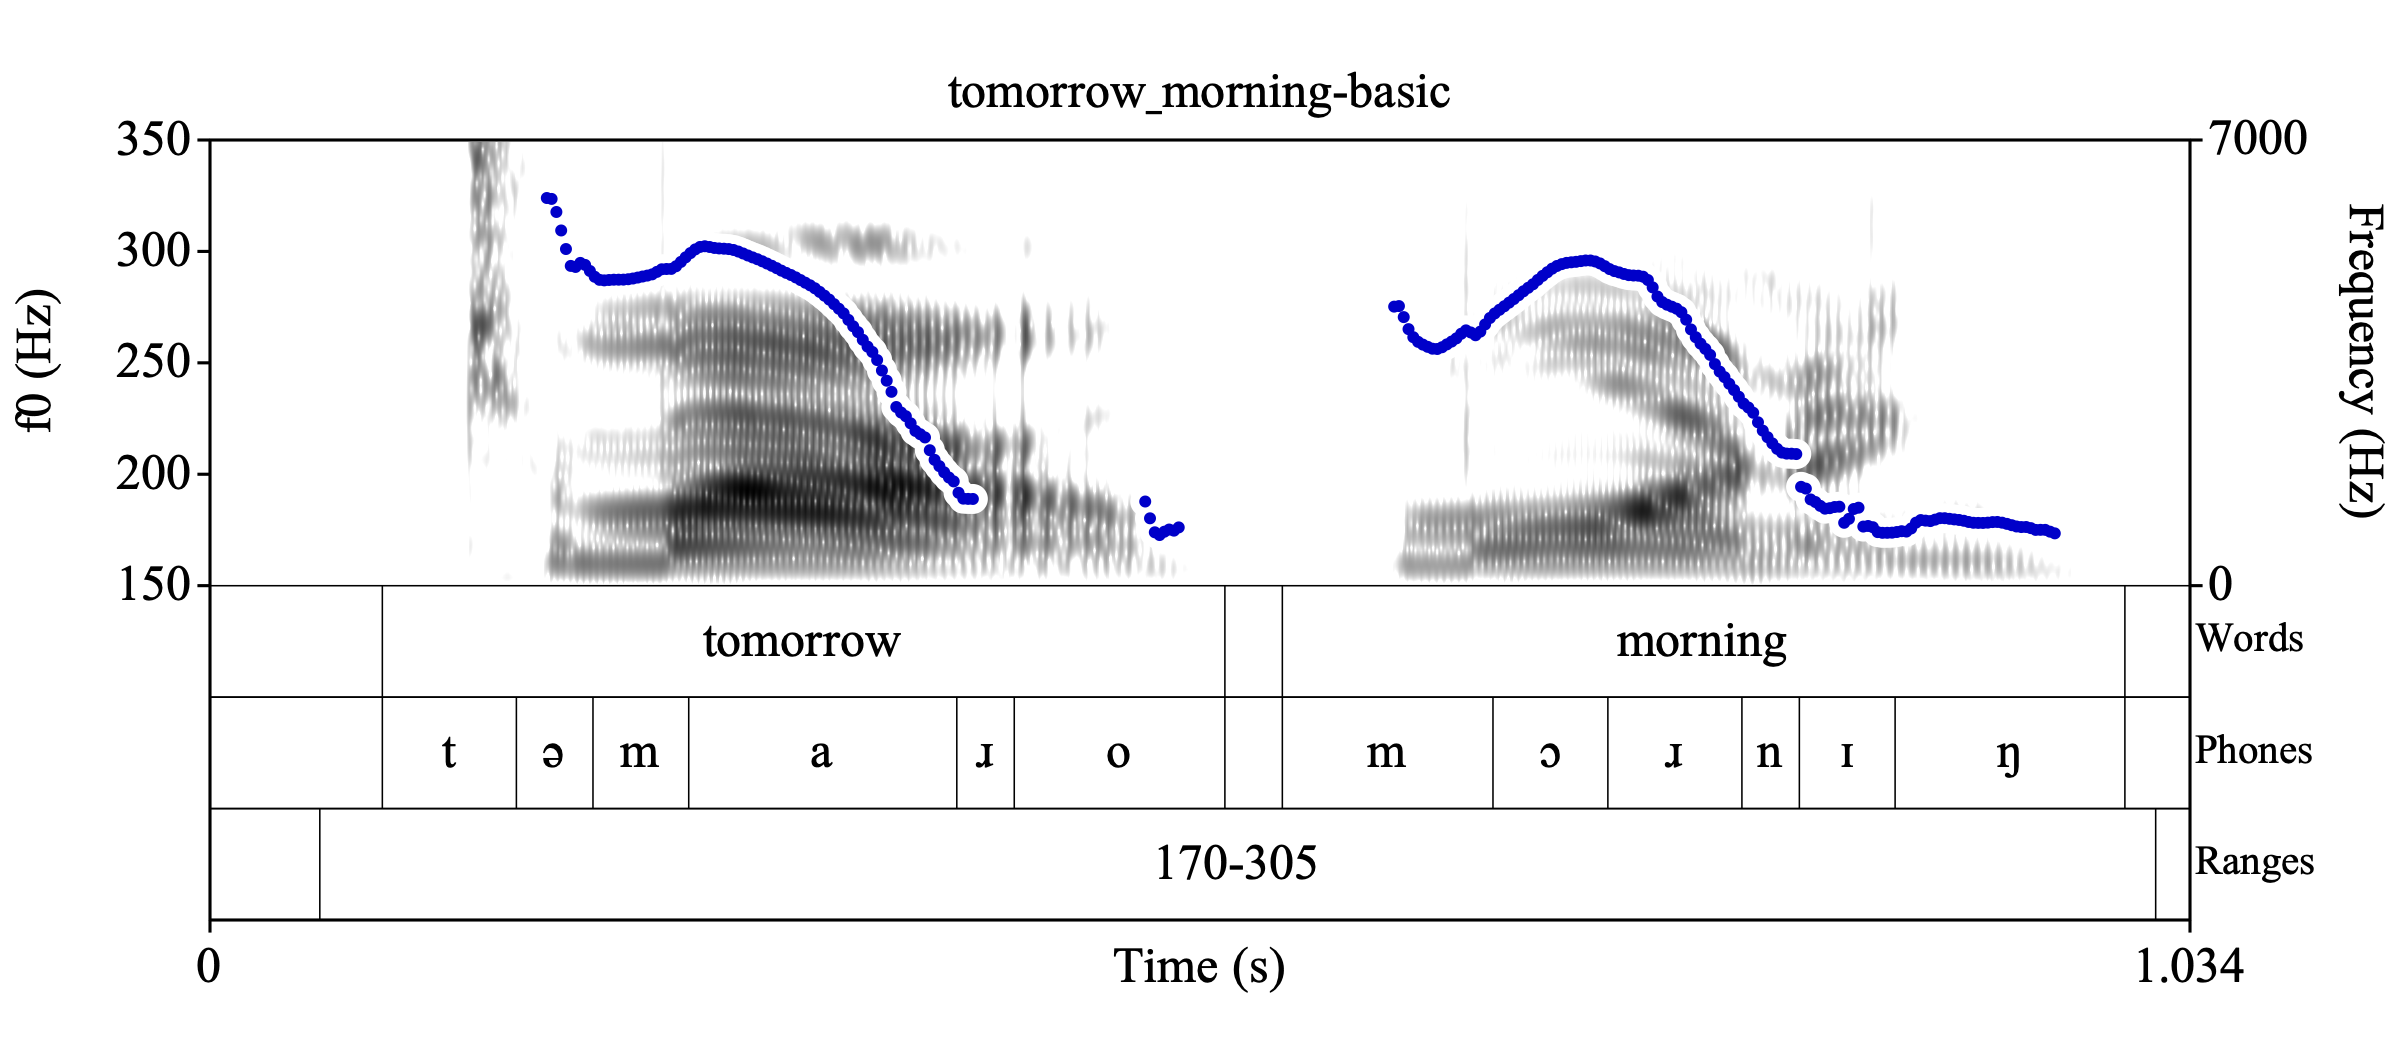
\includegraphics[width=.875\linewidth]{Ranges-tomorrow_morning-basic.png}
%
\caption{This example shows two short words produced with a silence between them, but sharing a single range.%
\label{fig:tomorrow_morning Ranges basic}%
\index{Annotated example, Ranges tier (basic)!tomorrow\_morning}%
}
\end{figure}

\subsection{Levels Tier}\label{sec:levels}

The Levels Tier (also called the \uline{Scaled \textbf{L}evels tier)} is a point tier that reflects the relative scaling of points in the Points tier within each successive range designated in the Ranges tier. The labels on this tier can be automatically added, using a script included with the Praat PoLaR plugin, once the Points tier and the Ranges tier have both been annotated. (Further instructions on using the plugin can be found in chapter \ref{ch:practical}.)

PoLaR uses 5 numbered levels, 1 to 5, where 1 is the lowest f0 band within the current range and 5 is the highest.\footnote{Some informal empirical support for this decision to employ 5 levels within the local range comes from Cole (p.c.), who found that four levels were not sufficient for synthesizing the basic contours of the MAE\_ToBI system, but five levels seemed to suffice.} A basic algorithm (one used by the PoLaR plugin script) divides the Hertz space of the current Range by 5. For example, for a hypothetical range of 100 to 150 Hz, the 50 Hz of the range would be divided into levels of 10 Hz:

\begin{itemize}
\item Level 1: ≥100, ≤ 110
\item Level 2: >110, ≤ 120
\item Level 3: >120, ≤ 130
\item Level 4: >130, ≤ 140
\item Level 5: >140, ≤ 150 \end{itemize}

The Levels value for a given point in the Points tier will be determined by that point’s f0 value in Hz (or the comma-override value), and where it falls in the current 5-part range. So, for this hypothetical range, a point between 140 and 150 Hz (e.g., 143.1) would be level 5, and a point between 110 and 120 (e.g., 119.7) would be a level 2.

Conceptually, the Levels tier divides the pitch space within given range (taken from the Range tier) into 5 equal bands or sub-ranges, as schematized in Figure \ref{fig:tomorrow_morning Levels basic}. In this example, the first point (falling during the [m] of “\langtext{tomorrow}”) corresponds to a turning point whose f0 in the pitch track is located in the top band (shown in red). Accordingly, this point gets assigned a 5 in the levels tier. Likewise the second point, which while slightly higher in f0, is still within the red band representing level 5. The following point, later in the [a] of “\langtext{tomorrow}”, corresponds to a slightly lower f0 that falls within the 4 band (shown in yellow), and therefore gets assigned a level 4. Points marked at both the end of “\langtext{tomorrow}” and the end of “\langtext{morning}” correspond to f0 points in the lowest band (in purple), and are assigned level 1. (Note that in this particular example, there is a point where the pitch tracker is unreliable during “\langtext{tomorrow}”, as the speaker’s voice has become creaky. Recall section \ref{sec:optional-f0-override-labels-for-annotating-pitch-points-without-a-reliable-f0-track}).

\begin{figure}[H]
\centering
%
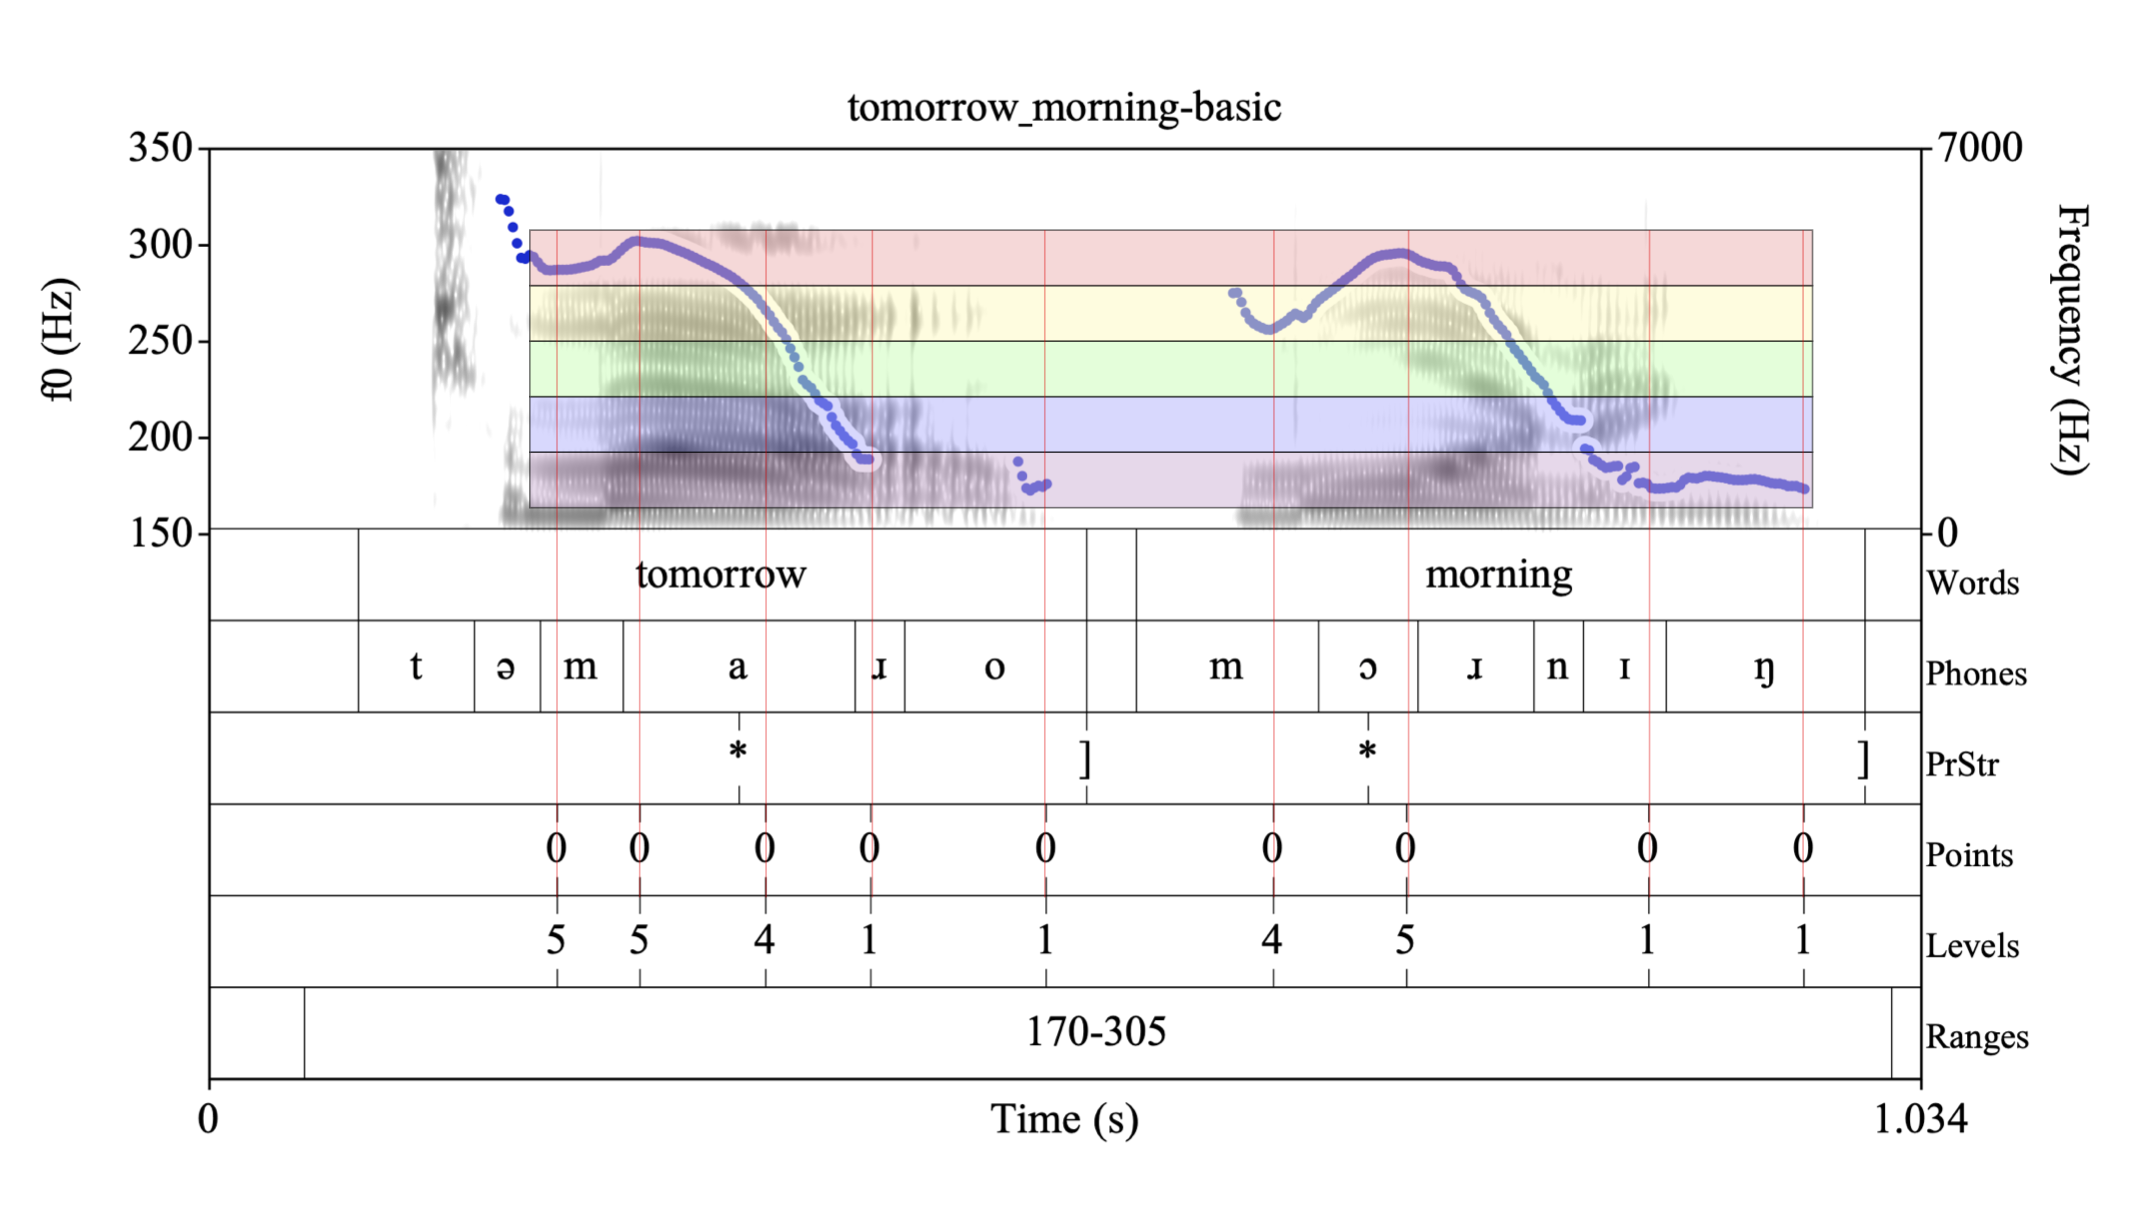
\includegraphics[width=.875\linewidth]{Levels-tomorrow_morning-basic.png}
%
\caption{A visual representation of the five pitch spaces corresponding to Levels annotation.%
\label{fig:tomorrow_morning Levels basic}%
\index{Annotated example, Levels tier (basic)!tomorrow\_morning}%
}
\end{figure}

The main advantage of the Levels tier is that it helps to encode (from the labels in the Ranges tier) what is perceived as categorically high vs. low. That is, the Levels tier captures the labeller’s intuition that a particular f0 event is produced high or low in the speaker’s current selected f0 range, as labelled in the Ranges tier (see section \ref{sec:ranges} above). This reflects the fact that raw f0 values do not adequately specify whether an f0 event realizes a high or a low tonal target, because speakers select different ranges (from within the overall range of possible f0 values that they can produce) for successive portions of an utterance. As noted above, PoLaR provides 5 levels on this tier, which can be automatically determined once the Ranges and Points tiers have been labelled.

For example, the file \texttt{no\_cigar}, shown in Figure \ref{fig:no_cigar Levels basic}, has 2 ranges annotated: 1) from 125-175 Hz for the word “\langtext{close}”, and 2) from 110-145 Hz for the word sequence “\langtext{but no cigar}”. Note that the pitch-accent-related point in the “\langtext{-gar}” of “\langtext{cigar}” is at around 140 Hz, so corresponds to a High in the range for “\langtext{but no cigar}” (as reflected in the level 5 designation, visually represented as the highest colored band in the right side of the figure), but it is only a bit higher (in absolute f0) than the point in “\langtext{close}” that is at 130 Hz, so corresponds to a Low (as reflected by the level 1 designation, visually represented by the lowest colored band in the left side of the figure) in the range for that word.

\begin{figure}[H]
\centering
%
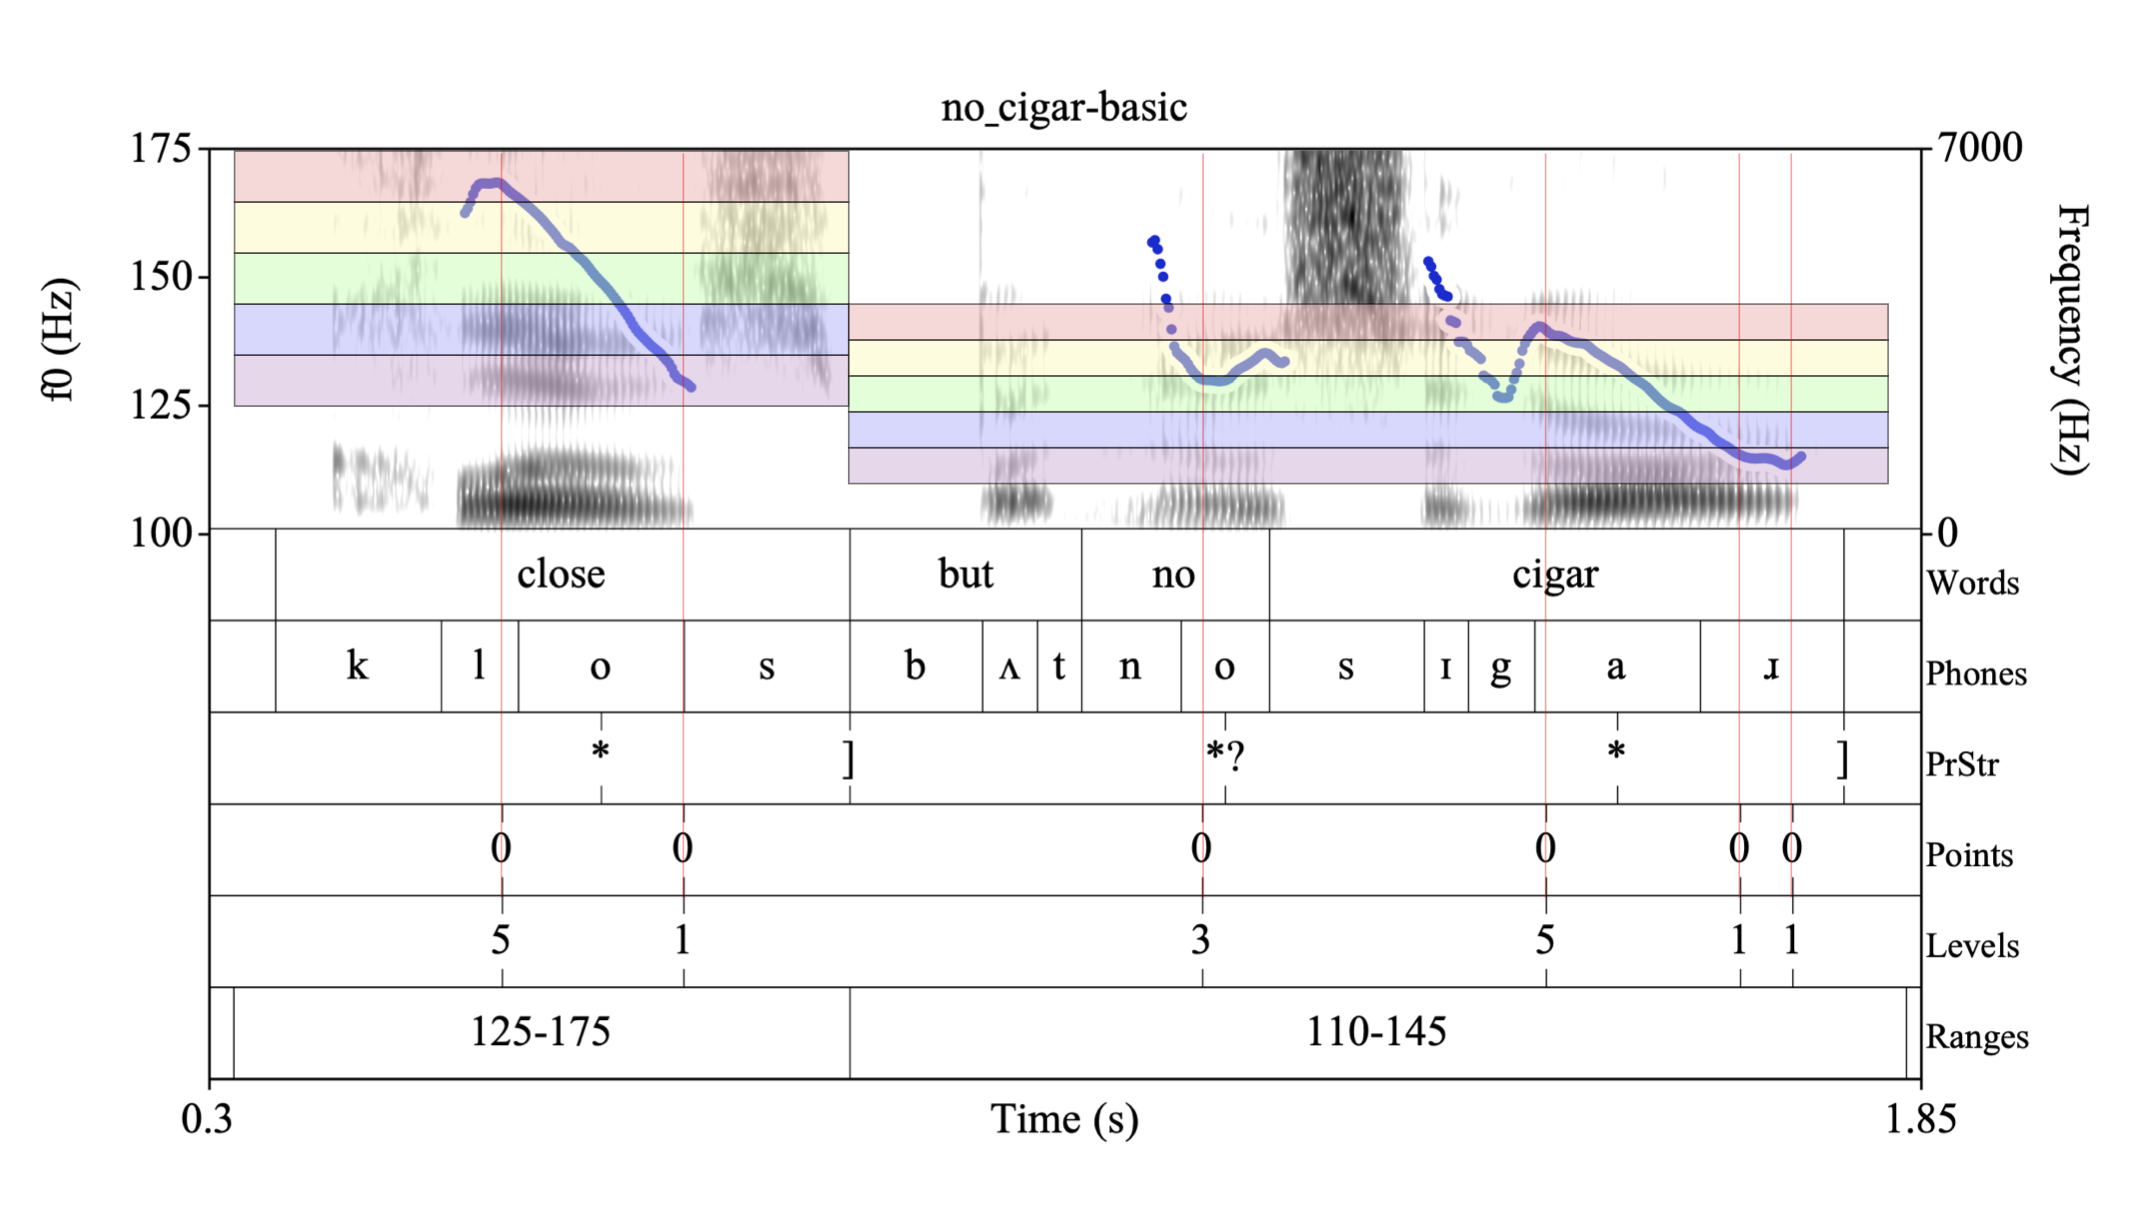
\includegraphics[width=.875\linewidth]{Levels-no_cigar-basic-rainbow.png}
%
\caption[\texttt{no\_cigar}, with Basic labels and overlaid colored bands.]{\texttt{no\_cigar}, with Basic labels on the Points, Levels, and Ranges tiers. The two sets of colored bands correspond to the scaled “level” values, with each set corresponding to one of the Range intervals.%
\label{fig:no_cigar Levels basic}%
\index{Annotated example, Levels tier (basic)!no\_cigar}%
}
\end{figure}


Given how Levels tier labels essentially normalize f0 values, these labels can be used for creating abstractions of the pitch contour, which can be compared directly, across items. To be specific, this production in Figure \ref{fig:no_cigar Levels basic} has 5-1-3-5-1-1 contour, while maybe a different production might have a 5-1-3-5-1-4 contour. What this Levels tier sequence allows for is an easy way to identify that the essential difference is in final pitch movement. In this way, Levels labels can serve as proxies for concepts like “high pitch” or “low pitch”, and may even be usable (in tandem with PrStr labels) to reconstruct phonological labels (e.g., ToBI \textlabel{H*} or \textlabel{H\%}.)

\section{Intonational Contours and Software-Based F0 Tracks}\label{sec:intonational-contours-and-software-based-pitch-tracks}

At this point, we have established how to annotate using PoLaR’s Basic labels, for each tier. Before moving on to the Advanced labelling system, this section takes us on an important digression to discuss the relationship between the intonational contours we aim to recover on the basis of PoLaR labels and the f0 tracks produced by software like Praat, since the f0 tracks are an important cue for labellers of the Points tier.

To review section \ref{sec:terminology}, the intonational contour is an abstract theoretical construct, and the software-based estimated f0 contour is a visualization, produced on the basis of particular settings and an algorithm. In other words, intonational contours and f0 contours are conceptually different. Intonational contours correspond to symbolic objects in the mind of a listener (thus not directly observable) that represent how pitch (a psycho-perceptual phenomenon) changes over time. On the other hand, f0 contours are visualizations corresponding to physical speech signals in which acoustic properties are measured in a programmatic way (which may make errors or produce contours that differ from the intonational contour).

A common goal for an annotator is to keep track of how pitch changes over time —by annotating key elements of the intonational contour— using both auditory perception as well as the f0 contour visualizations (a.k.a. “f0 tracks”). While the f0 track produced by software like Praat\footnote{Note that Praat uses the phrasing “pitch contour” to refer to what we call the “f0 track” or “f0 contour”.} often accurately reflects changes in the intonational contour (hence its usefulness to annotators), f0 tracks are also often discontinuous, jerky, and error-prone in a way that can mislead an annotator if they are not careful. This is because f0 tracks are produced by a mechanistic algorithm that has various adjustable settings (discussed below; see also \href{https://www.fon.hum.uva.nl/praat/manual/Intro_4_2__Configuring_the_pitch_contour.html}{§4.2 of the introductory tutorial to Praat}), and these settings often need to be adjusted. (For more information about how software like Praat produces f0 tracks, see §5 of \citealt{weenink20}.)

In what follows, we will discuss f0 tracks and intonational contours further, including how intonational contours can be approximated, and how f0 tracks are commonly disrupted and how to see “past” disruptions. We will also provide specific guidance and methods for dealing with f0 tracks when doing intonational labelling (in particular, when labelling the Points tier).


\subsection{Intonational Contours and Straight Line Approximations}\label{sec:intonational-contours-and-straight-line-approximations}

As just discussed, the f0 track (i.e., the software-produced estimate of f0 movements, which is produced by an algorithm on the basis of the acoustic signal) consists of a very large number of pitch values (by default, Praat estimates 100 f0 values per second). The idea behind the Points tiers labels is that, at an abstract level, a pitch contour can be defined by a relatively much smaller number of observations (perhaps just a handful for a short utterance). Following in the footsteps of the IPO tradition (e.g., \citealt{t-hartcollier75} and \citealt{t-hart-90}), we have described this in terms of “straight line approximations” (as discussed in section \ref{sec:identifying-necessary-points-labels-with-straight-line-approximations}). In this section we will discuss more on the relationship of Points tier labels and straight line approximations.

A major insight of the IPO framework is that straight line approximations based on a very small number of f0 turning points can be perceptively the same as original recording. (The IPO approximation process is described in works like \citealt{dutoit97} and \citealt{rao12}.) When annotators create a straight line approximation, they are essentially reducing an f0 track to the core pitch turning points. This regularly requires the annotator to ignore movements in the f0 track that are not mirrored in auditory perception (such as those due to microprosody or software errors, as described in sections \ref{sec:software-effects}–\ref{sec:voice-quality-effects}). It also involves ignoring some of the more gradual f0 turning points that define scoop- or dome-shaped contours (instead reducing them to maybe one or two points). (That is, some sudden f0 changes can be ignored, and some gradual changes can be reduced to single pitch turning points.) Repeating some of what is in section \ref{sec:identifying-necessary-points-labels-with-straight-line-approximations}, we provide some guidance on how to identify how many Points labels are necessary. The first piece of guidance we provide here is that we suggest adding Points labels one at a time –erring on the side of over-labelling– to faithfully reproduce the major movements in the f0 track. The second is, to cull the labels that are unnecessary for producing a faithful straight line approximation. When in doubt whether a Point is necessary or superfluous, labellers ought to compare straight line approximations where one includes the Point and the other does not. (If they sound perceptually the same, the Point can be removed.) 

Consider the examples in Fig. \ref{fig:enemy original and resynth} below. The original (more true-to-form) pitch track (on the left) depends on identifying pitch points at a regular (and very high) interval, while the straight-line approximation depends on just the six points identified in the PoLaR Points tier. Even to a trained ear, the resynthesized utterance in the figure on the right is perceptibly the same. In this way, PoLaR can be seen as enabling researchers to remove all but the pitch points “that matter”. PoLaR provides a means (the Points tier labels) to identify the coordinates (for axes of time and pitch space) that can define the intonational contour, and the PoLaR plugin for Praat can be used to resynthesize straight line approximations on the basis of those Points labels. (See section \ref{sec:identifying-necessary-points-labels-with-straight-line-approximations} for more details about this.)

\begin{figure}[H]
\centering
%
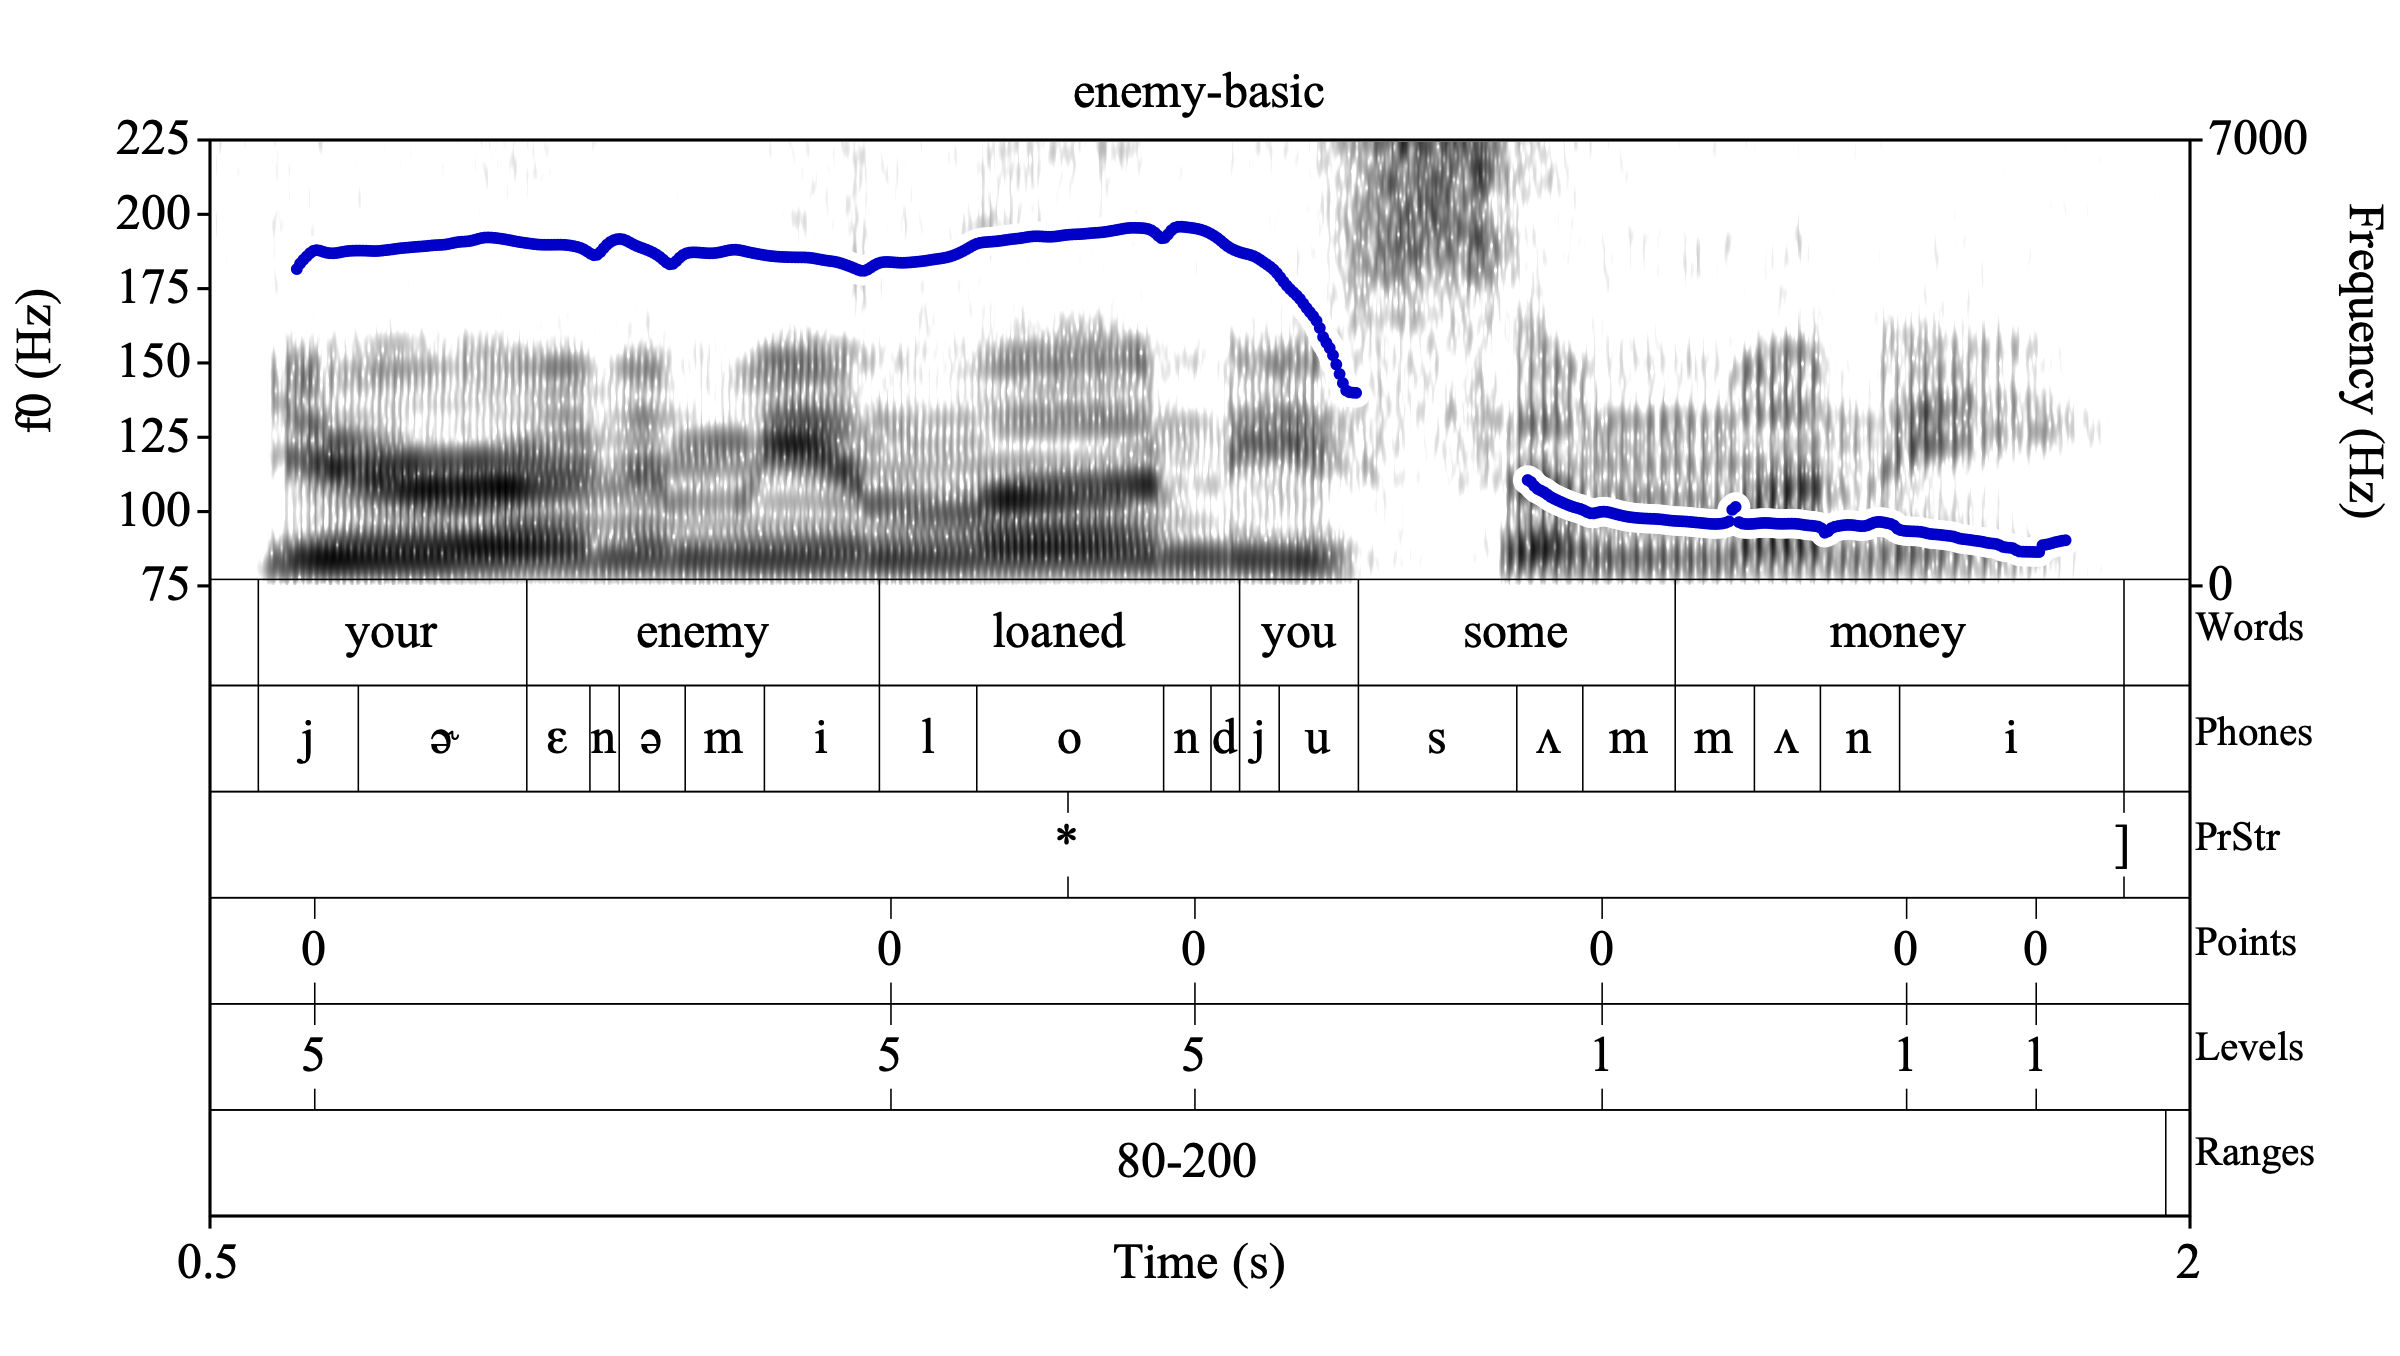
\includegraphics[width=.485\linewidth]{Contours-enemy.png}~~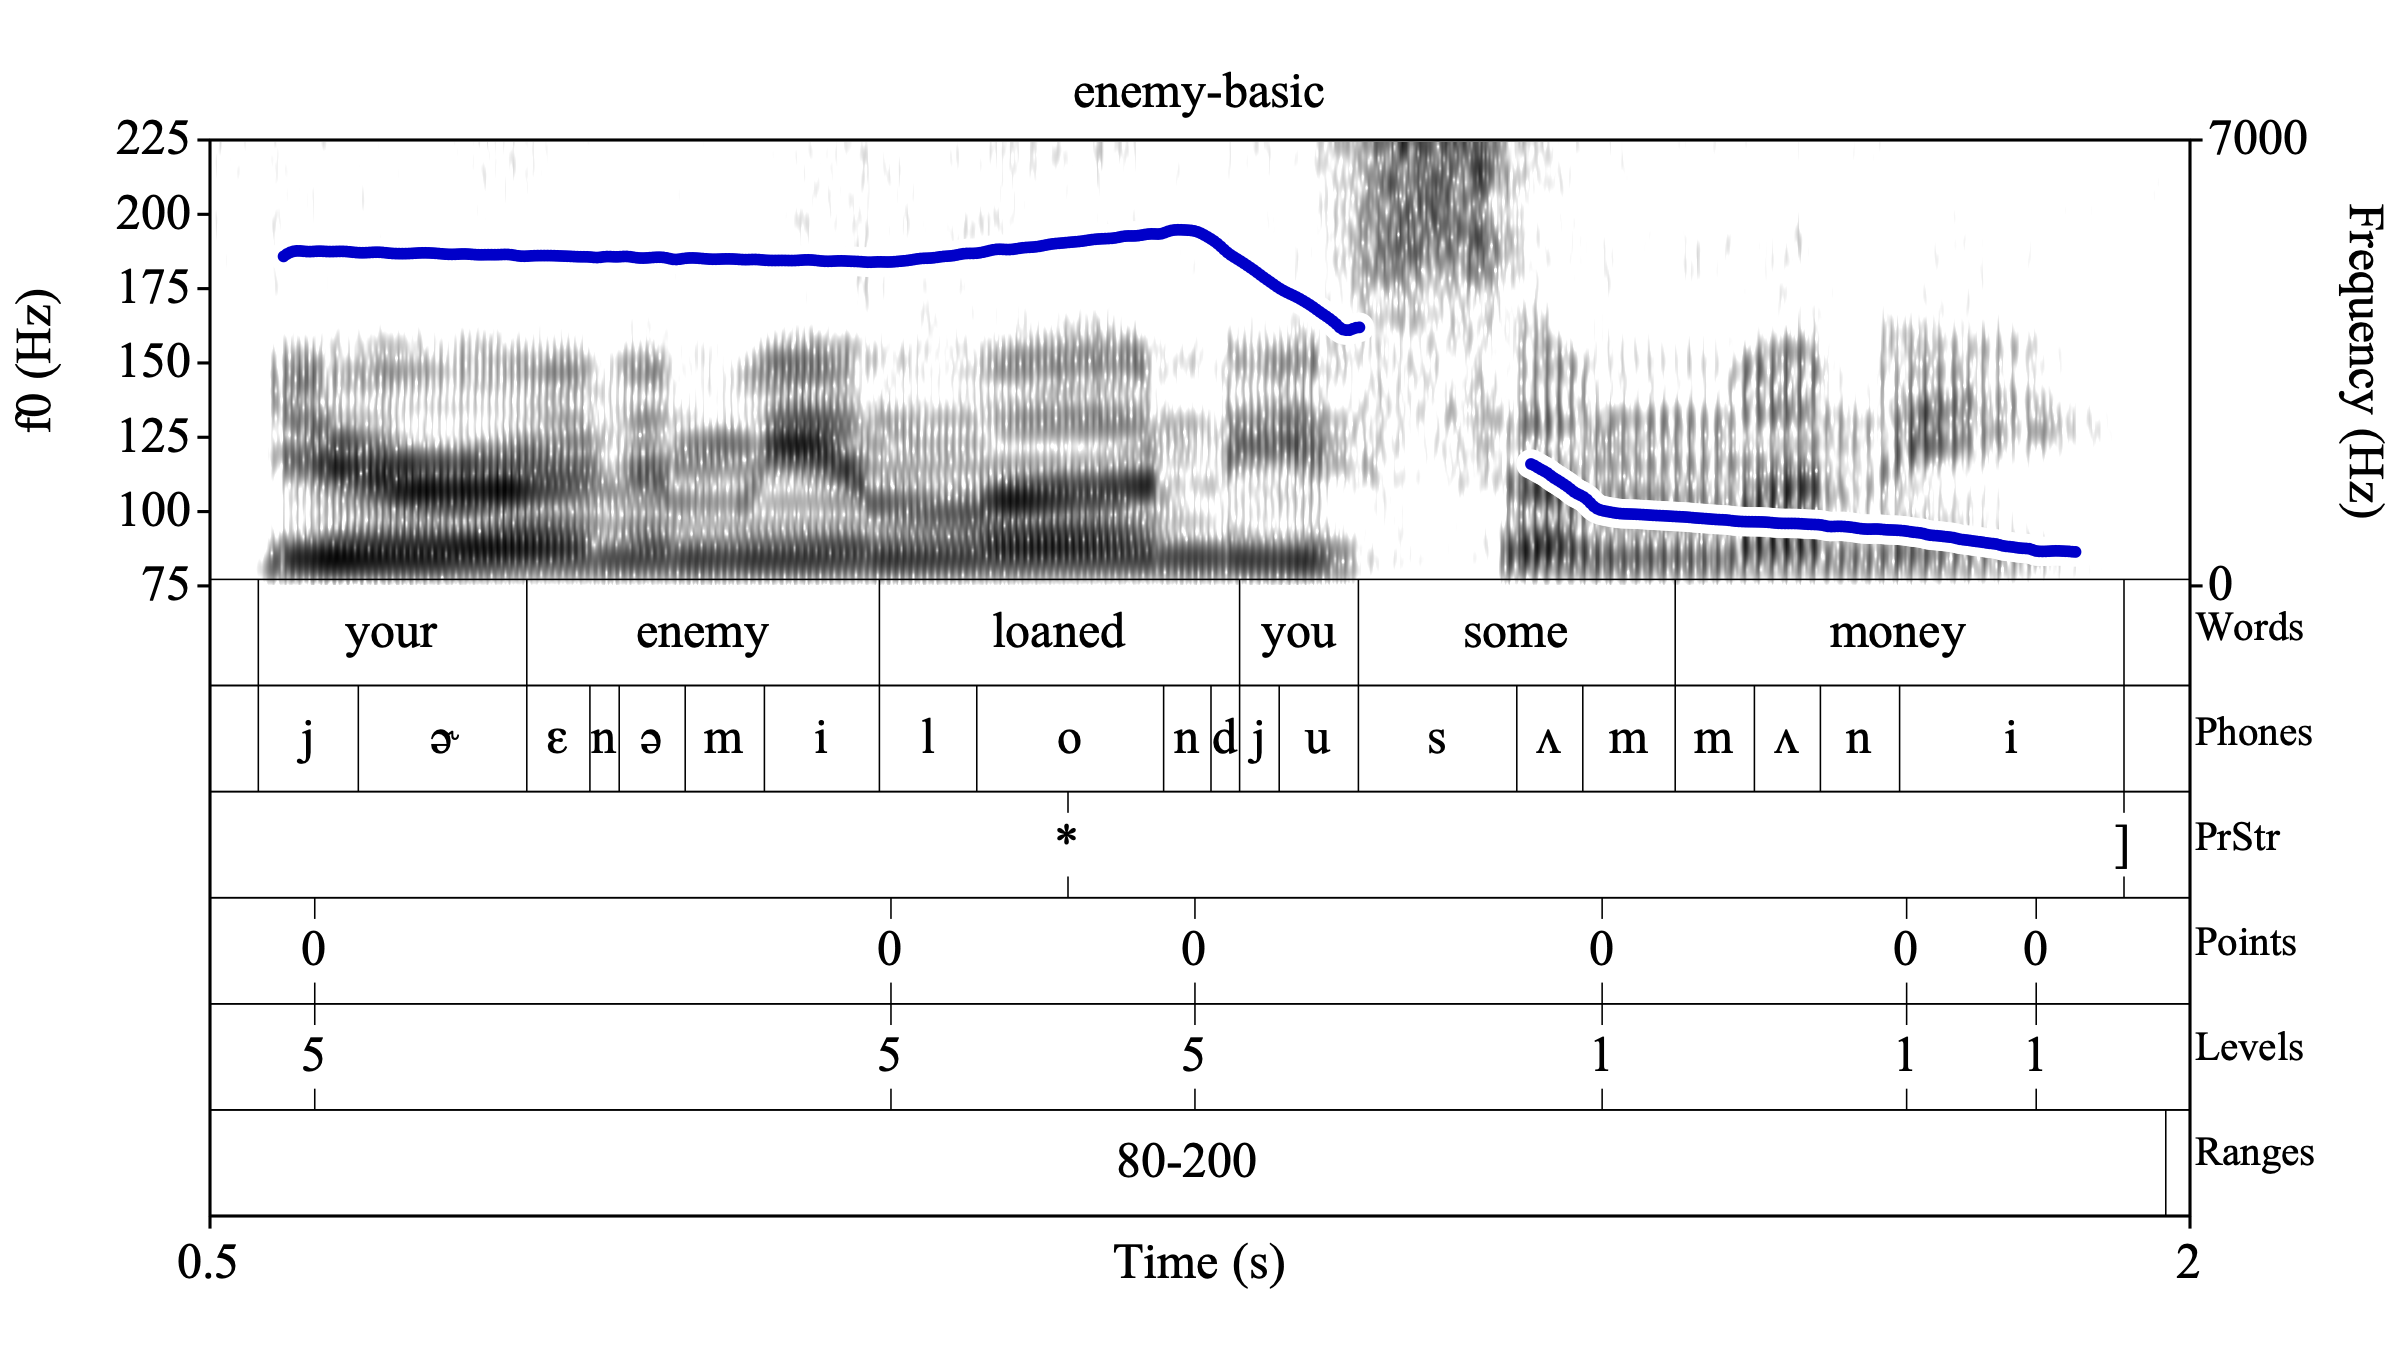
\includegraphics[width=.485\linewidth]{Contours-enemy-resynth.png}
%
\caption{A recording with PoLaR labels and its resynthesized straight line approximation, created with a script from the PoLaR plugin in Praat.%
\label{fig:enemy original and resynth}%
}
\end{figure}

Even with such an impoverished version of the pitch track (such as \texttt{enemy-resynth}), and even to a trained ear, the “real” and “resynthesized” examples can be indistinguishable. On the other hand, removing some of these remaining turning points may result in a somewhat “unnatural” sound (in the sense that, at least, a trained ear could distinguish the resynthesized version from the original). Given that this straight line approximation sounds both natural and identical to the original, we argue that our Points tier annotation of six pitch points in Fig. \ref{fig:enemy original and resynth} is sufficient to capture the meaningful turning points. This same technique of manipulating pitch into a straight line approximation can be applied to any recording, to see whether the correct number of Points have been labelled.

Practically speaking, we assume that experienced labellers will be able to distinguish significant turning points from noisy variation, but caution is urged in eliminating those that would impact the shape of the contour. Our experience with the Tonal Center of Gravity dictates that individual Turning points are not perceptually salient; it is the set of turning points that creates a perceptually useful shape. 

In this way, using the Points tier labels to construct a straight-line approximation of the f0 track (which itself is based on the acoustic signal) can be used to help identify the shape of the (abstract phonological) intonational contour.\footnote{Note: this series of acoustic cues in the signal does not, for various reasons (including the phonetics-phonology interface, technical abilities of the pitch tracking software, microprosody, etc.), perfectly reflect the intonational contour, which is an abstract representation (defined in terms of phonological categories and structures).} As such, these straight line approximations have the potential for understanding more about the phonological representation of intonational contours.

\subsection{Sources of f0 track disruptions}\label{sec:a-brief-overview-of-sources-of-pitch-track-disruptions}

As mentioned, while the f0 track is often reflective of the perceptual changes in pitch, there are also regular ways in which the f0 track can differ from the intonational contour. For example, an annotator may perceive the pitch of a portion of the utterance as being steady or moving fluidly, while the f0 track of that region shows a discontinuous f0 contour or one that suddenly jumps up\slash down. Thus, if the labeller over-trusts the visualization in the f0 track (overriding how their auditory pitch perception), this may cause a labeller to label extraneous Points labels to capture movements that are not actually part of the speaker’s intonational contour. (Conversely, the visualization may not seem to show f0 movements even where a labeller auditorily perceives one.) In this section, we discuss some of the more common specific f0 tracking problems that occur, the contexts in which they are likely to arise, and the conventions that have arisen over the years among prosodic labellers for dealing with them.

One class of problems occurs when the software-based f0 estimator is disrupted, leading to breaks in the f0 track. A second kind of problem occurs when contextual factors in the speech\slash recording context distort or influence the f0 track, even though a listener’s perception of the pitch contour is not disrupted by these events. Both of these scenarios can challenge the labeller by complicating the issue of determining where Points labels should(n’t) be added.

When in doubt, the annotator is encouraged to \emph{trust their perception}, because the human mind is especially well-tuned to compensate for these disruptions (producing the abstract and “smoothed” intonation contour, on the basis of intonational competence) while software like Praat is designed to keep track of all f0 movements.

\subsubsection{Software effects}\label{sec:software-effects}

One very common way in which f0 tracks end up as inaccurate (meaning not reflecting listeners’ perception of the pitch) has to do with software settings. Most speech applications (such as Praat) must be calibrated regularly (e.g., re-calibrated for each speaker) to get accurate f0 displays.

An example of settings that can greatly impact f0 tracks is the Pitch range minimum\slash maximum values (in Praat, these are found in Pitch > Pitch settings, in an editor window, when viewing Sound objects). What these settings do is tell the algorithm what the minimum\slash maximum \emph{possible} f0 values are; that is, the algorithm will not entertain the possibility that the f0 values dip below the minimum or above the maximum. As such, if the minimum is set too high (e.g., the minimum is set to 100Hz but the actual f0 gets as low as 75Hz), the software will often produce an f0 track with plotted values that are too high (e.g., plotting f0 values at 160Hz where they ought to be 80Hz; see also §\ref{sec:pitch-halving-and-doubling}). Annotators are encouraged to tailor the Pitch range values for speakers, noting that deeper voiced people typically stay within a range of around 60-300Hz, and higher voiced people typically stay within a range of around 100-500Hz, but this can vary quite a bit from person-to-person (and even from recording to recording).

In addition, Praat (\citealt{praat}) provides various other pitch-related settings, for which we provide values we have found to be helpful in doing intonational analysis of human speech; these are the settings used to produce the figures of f0 tracks in this monograph. (The menus referenced below are found in an editor window).

\begin{itemize}
\item Settings for Time Step analysis (found in \texttt{View> Time step settings}\ldots):
	\begin{itemize}
		\item Time step strategy = fixed
		\item Fixed time step (s) = 0.0025
	\end{itemize} 
\item Advanced Pitch settings (found in \texttt{Pitch> Advanced pitch settings}\ldots):
	\begin{itemize}
		\item Max. number of candidates=15
		\item Very accurate=true
		\item Silence threshold=0.03
		\item Voicing threshold=0.5
		\item Octave cost=0.05
		\item Octave jump cost=0.5
		\item Voiced/Unvoiced cost=0.2
	\end{itemize}
\item[] (\textit{You may find it beneficial to adjust these settings further, in particular recordings, to minimize spurious\slash inaccurate f0 measurements. However, doing so may result in f0 tracks that look different from the ones in this monograph.})
\end{itemize}

Changing these settings may affect the f0 track – for example, changing the voicing threshold and octave jump costs can lead to f0 dropout or spurious f0 readings. This should be taken to reinforce the fact that f0 tracks are meant only as a guide to annotators, and annotators are encouraged to diverge from it when their auditory perception suggests. 

While adjusting software settings (especially Pitch Range minimum\slash maximum) is a way to counteract f0 track disruptions, some f0 disruptions cannot be amended to yield an accurate f0 track, due to insurmountable interference from environmental\slash recording factors (e.g., background noise). In these cases, as described in section \ref{sec:optional-f0-override-labels-for-annotating-pitch-points-without-a-reliable-f0-track}, labellers are encouraged to use their intuition and perception to note an f0 estimate, if appropriate and possible. 

\subsubsection{Pitch halving and doubling}\label{sec:pitch-halving-and-doubling}

Sometimes during a recording, the f0 track will suddenly jump or fall – with the measured f0 jumping from say 199Hz to 97Hz (or vice-versa) from one measured f0 point to the next. When suddenly dropping down by a factor of 2, this is pitch halving. Conversely, when suddenly jumping up by a factor of 2, this is pitch doubling. (The factor of 2 difference is due to how Praat measures f0. Because these jumps are related to the f0 measuring algorithm, they are not always exactly a factor of 2; however, factor-of-2 jumps\slash drops are especially common.) 

In other words, pitch halving and pitch doubling involve a change in measured f0 is immediate and significant – faster than the vocal folds can typically change. An example of pitch halving is given in Figure \ref{fig:to volunteer-halved f0-tracking}, and an example of pitch doubling is given in Figure \ref{fig:rutabaga f0-tracking}.

\begin{figure}[H]
\centering
%
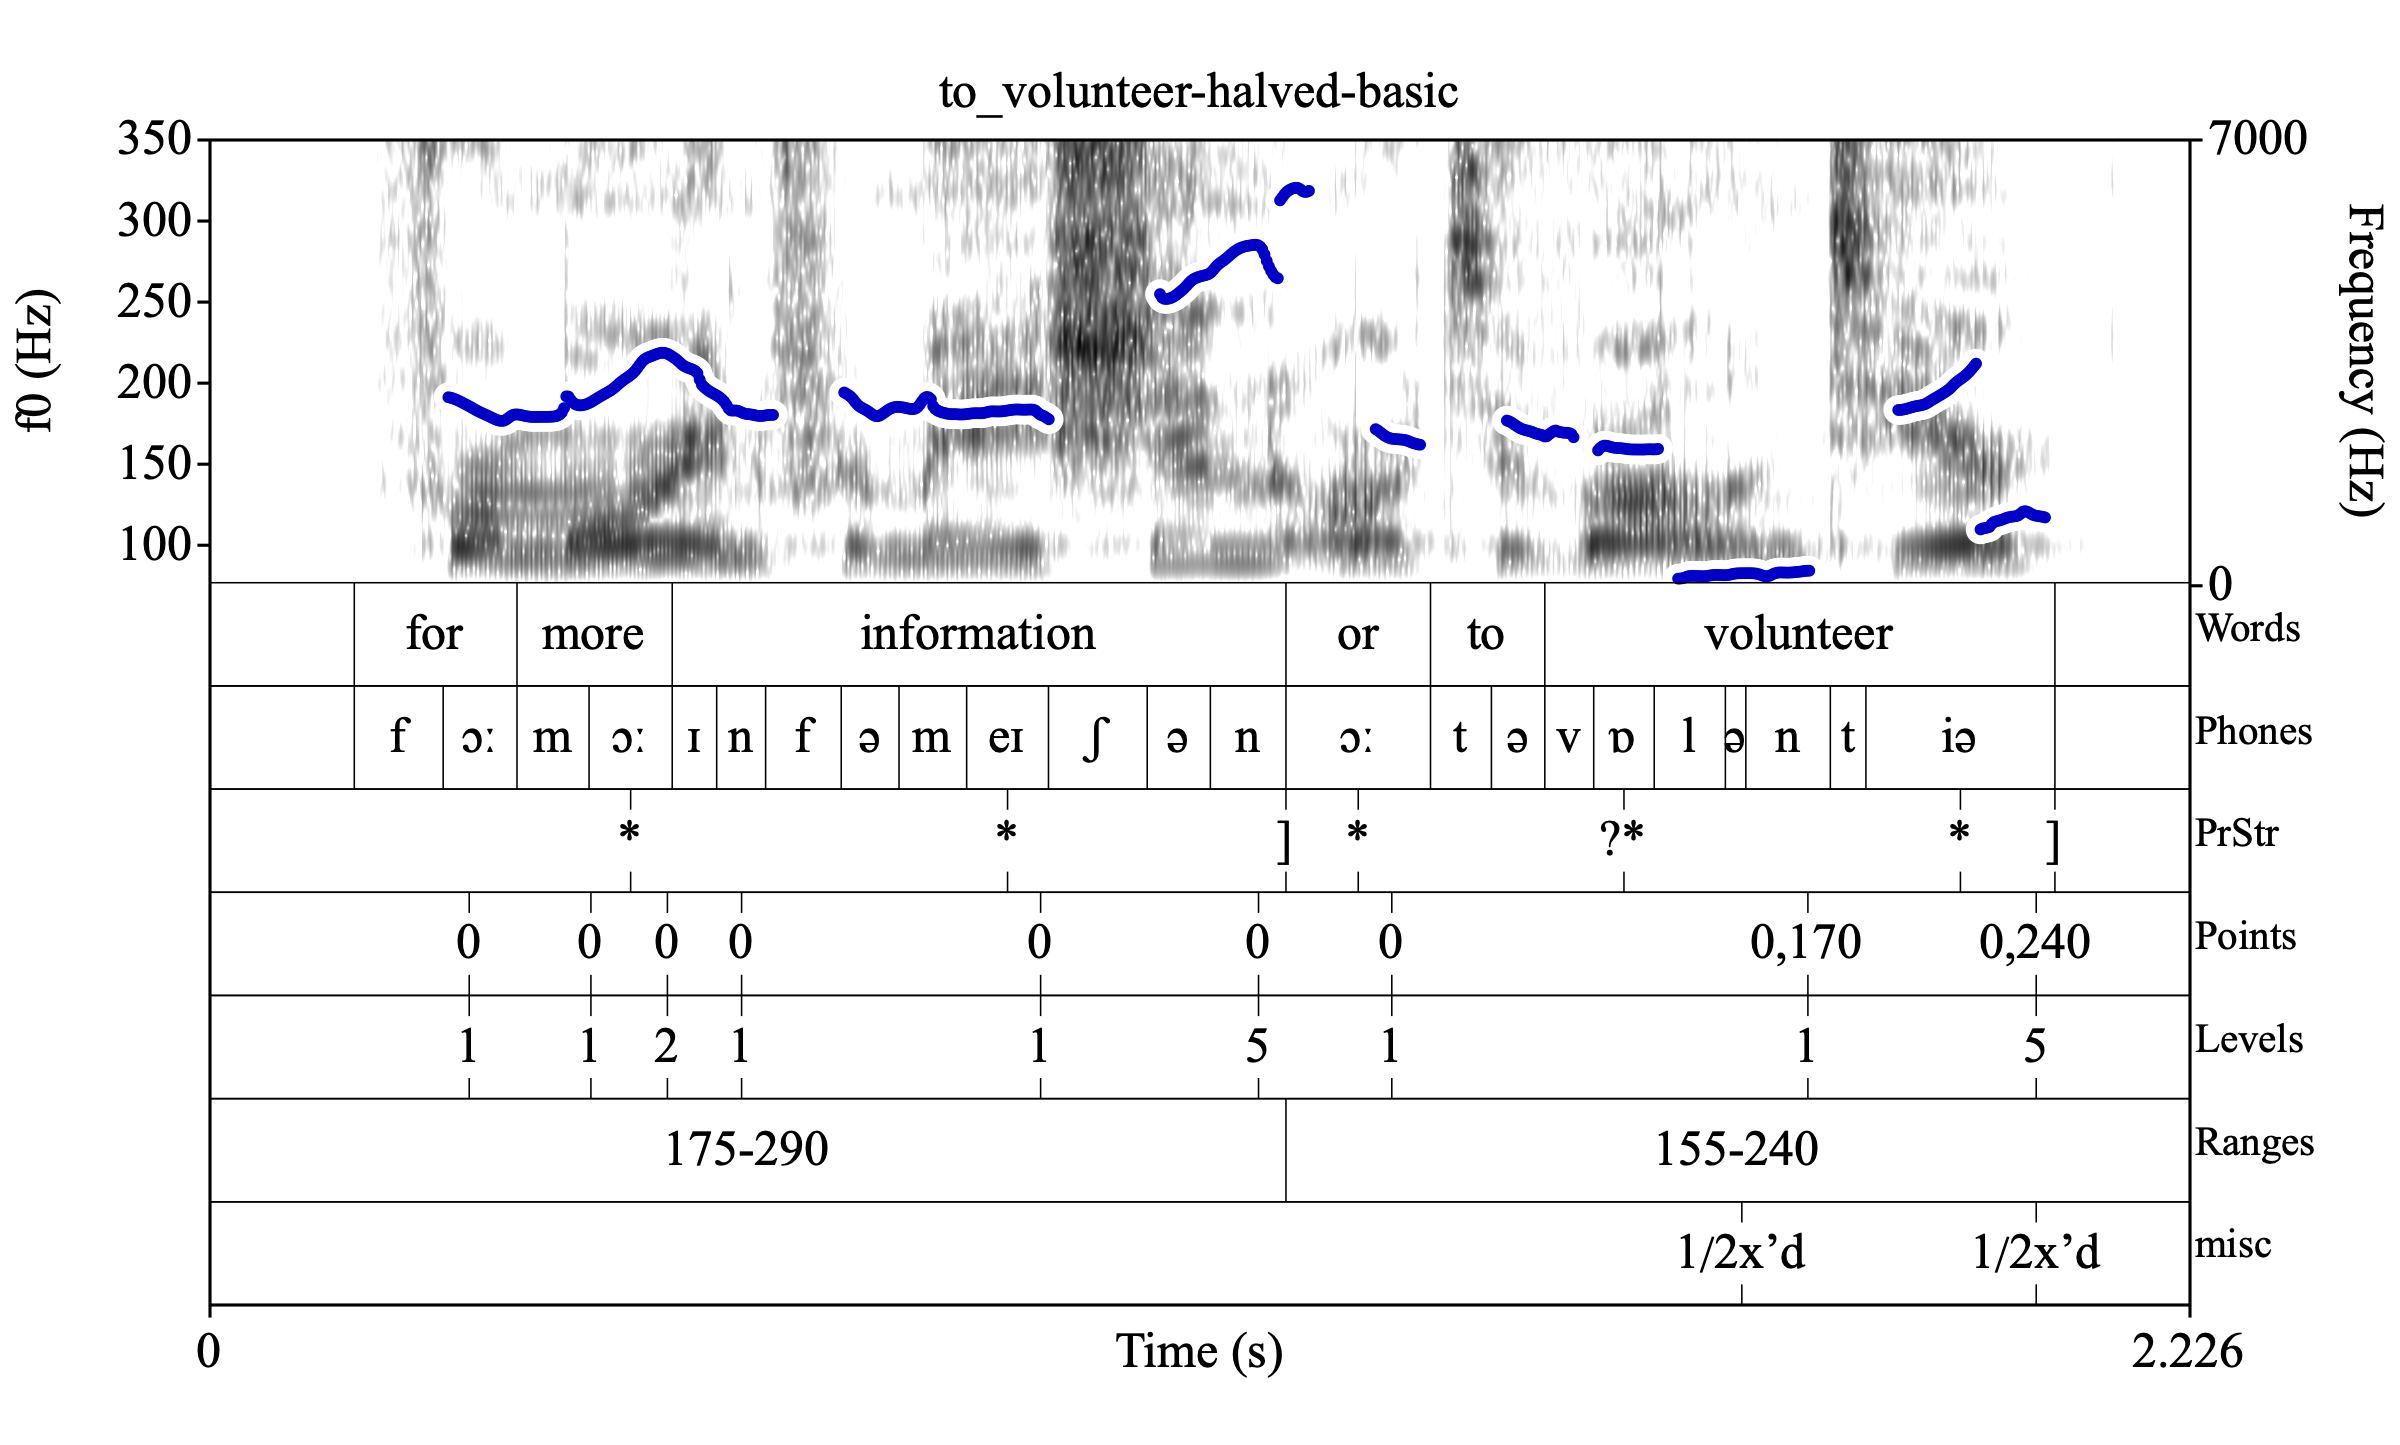
\includegraphics[width=.875\linewidth]{Appendix-to_volunteer-halved.png}
%
\caption{Example of pitch halving.%
\label{fig:to volunteer-halved f0-tracking}%
\index{Annotated example, f0 tracking!to\_volunteer-halved}%
}
\end{figure}

\begin{figure}[H]
\centering
%
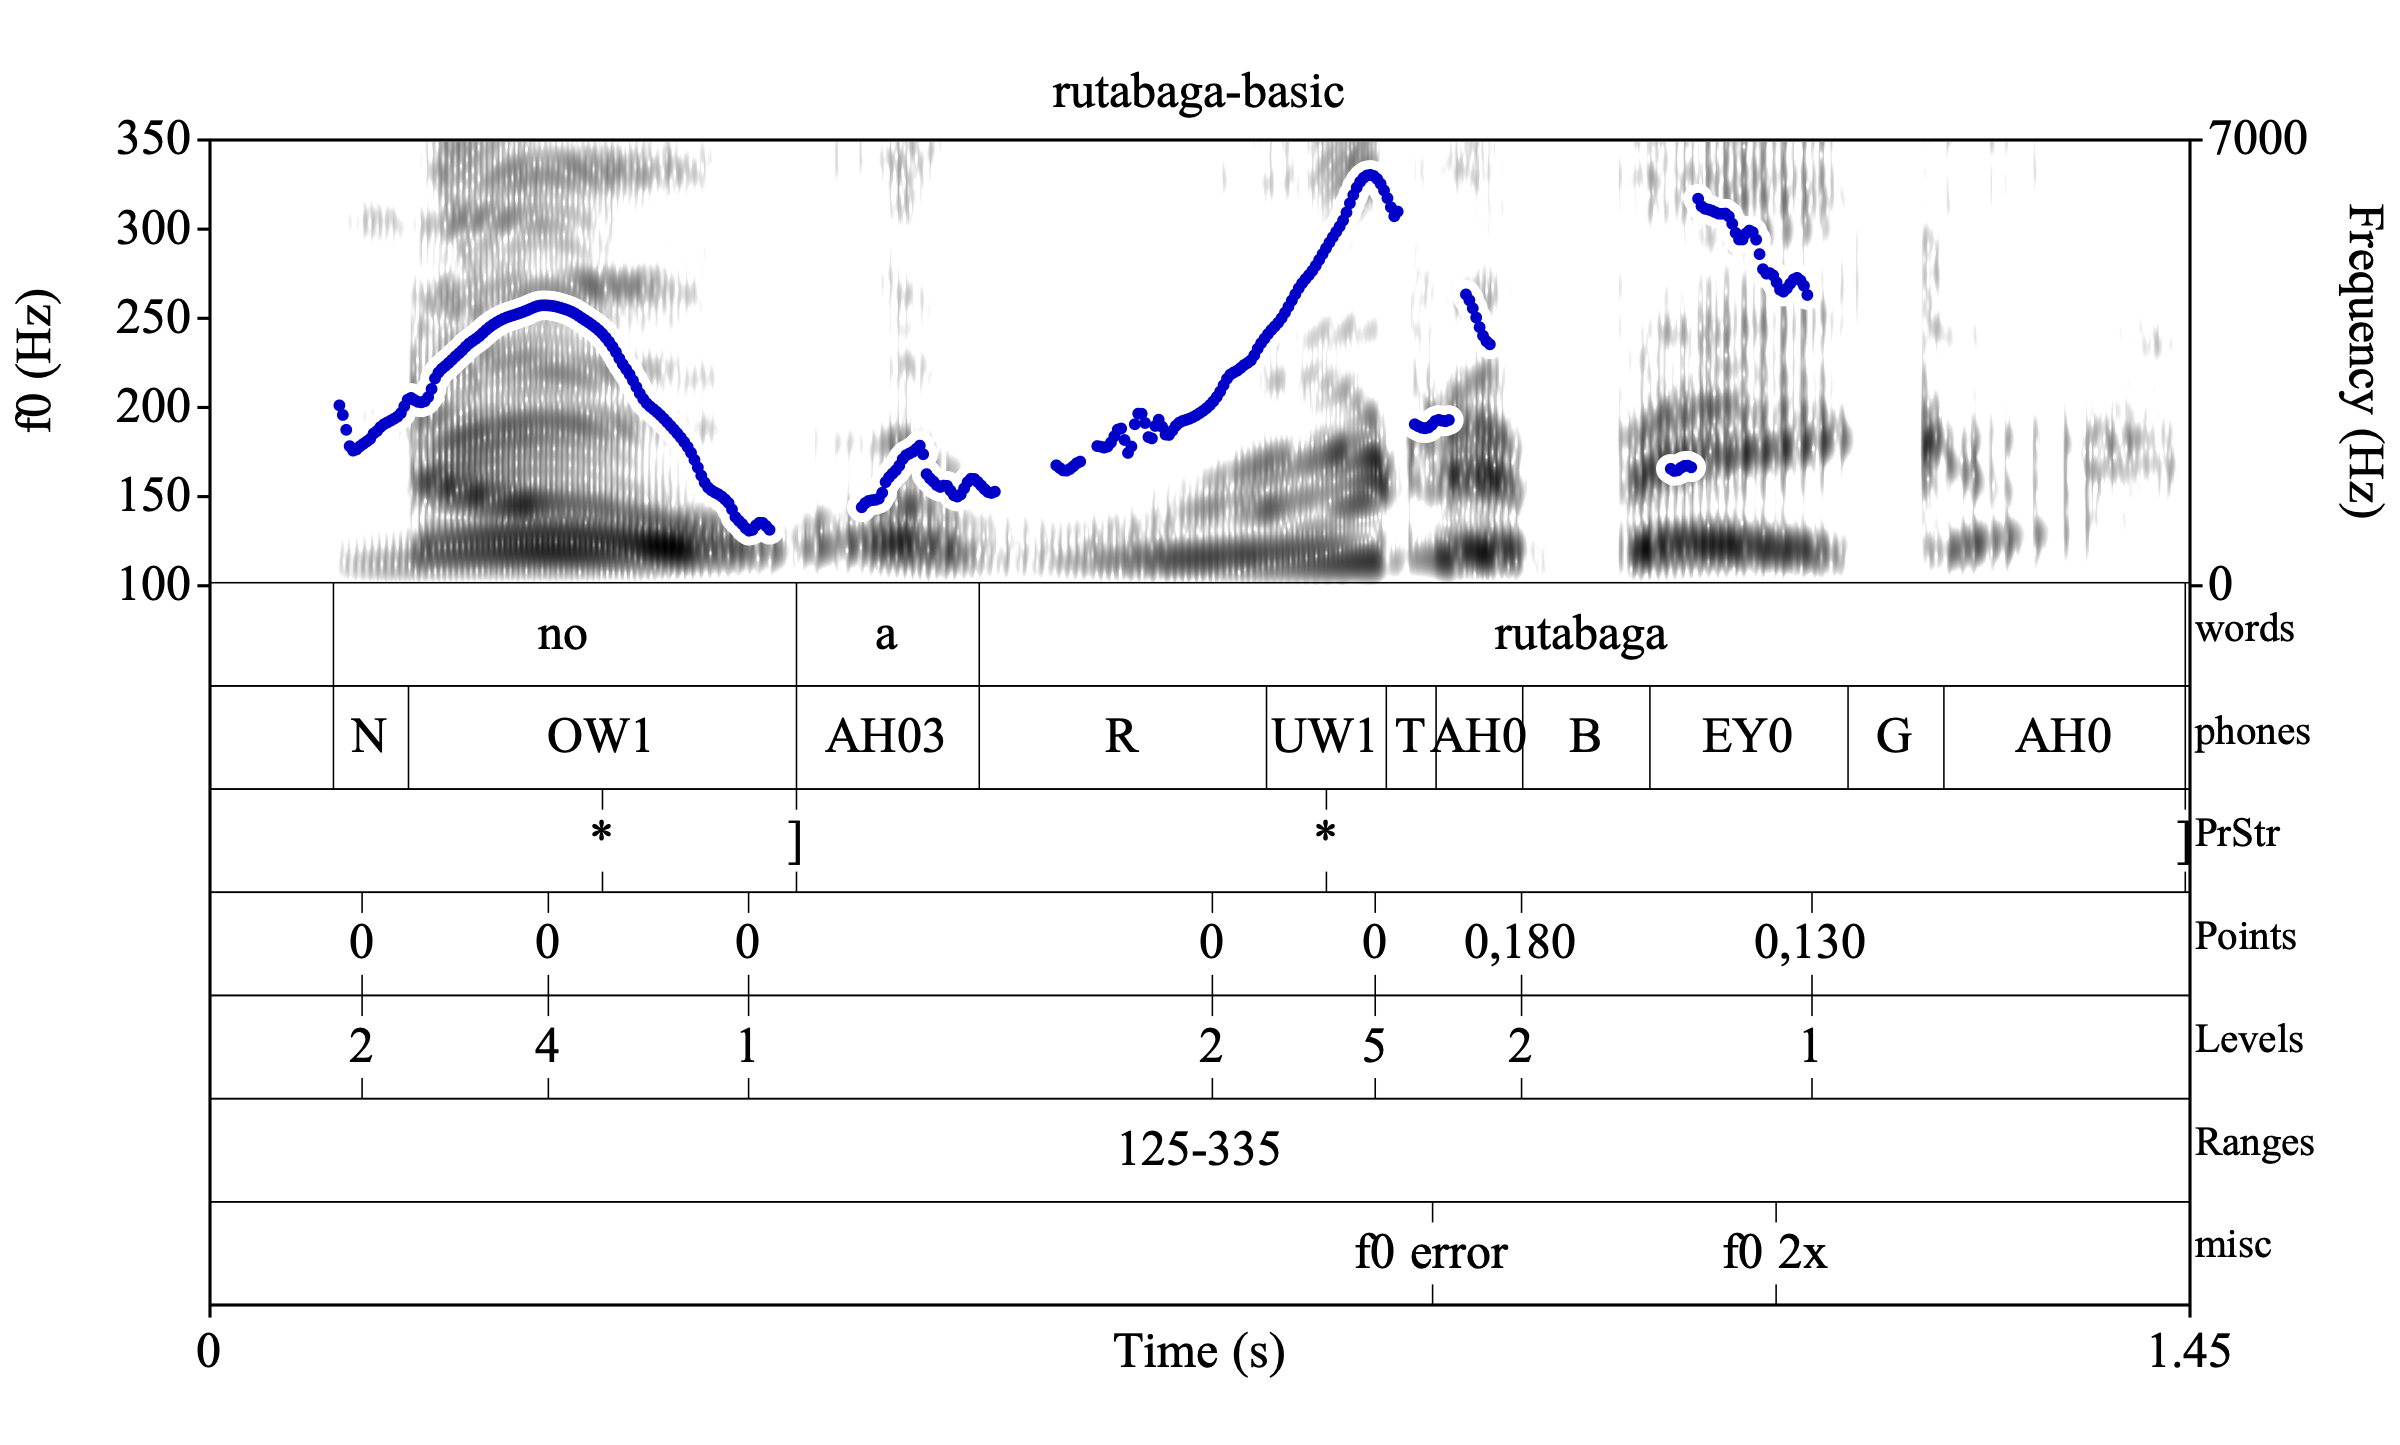
\includegraphics[width=.875\linewidth]{Contours-rutabaga-basic.png}
%
\caption{Example of pitch doubling.%
\label{fig:rutabaga f0-tracking}%
\index{Annotated example, f0 tracking!rutabaga}%
}
\end{figure}

We provide some hints to help identify what is “immediate and significant”, a labeller can rely on.
First and foremost, a labeller should trust their auditory perception. If the labeller perceives that the pitch is locally low, but the f0 track looks locally high, this could be due to pitch doubling; for example, at the end of “\langtext{rutabaga}” in Fig. \ref{fig:to volunteer-halved f0-tracking}, the pitch is perceived to continually fall, but it shows as almost as high as the preceding peak. Similarly, if the f0 shows a low that sounds high to the labeller, this may be halving. In these cases, the f0 tracker commonly measures f0 values that are either half (e.g., the pitch tracker shows 70 Hz, where listeners perceive pitch corresponding to 140 Hz) or double (e.g., the pitch tracker shows 140 Hz, where listeners perceive pitch corresponding to 70 Hz) the “true” pitch for the speech.

A second way is to try changing the pitch range settings. If the pitch range settings are set to 100-200Hz, but the true f0 max is 250Hz, any f0 that is truly between 200Hz and 250Hz will be mis-measured – often as pitch halving, showing as 100-125Hz. This is because, if a speaker reaches a peak f0 over 500Hz but your maximum is set at 400Hz, the f0 tracker will be forced to estimate points within that range. Adjusting the setting for the pitch range maximum to be 250Hz will often resolve this sort of pitch halving. However, there are cases of pitch halving\slash doubling that persist even when the pitch range is set appropriately (such as Fig. \ref{fig:rutabaga f0-tracking}).

The third way we name here to check perception is to make use of the tool for resynthesizing straight line approximations (as described in section \ref{sec:identifying-necessary-points-labels-with-straight-line-approximations}). In Fig. \ref{fig:to volunteer-halved f0-tracking}, there are no Points labels during the pitch-halved regions, and resynthesizing yields a recording that sounds like the original. Had the drop in measured f0 been faithful to a drop in the true f0, such a resynthesis without Points labels encoding the drops would sound like a different contour. For Fig. \ref{fig:rutabaga f0-tracking}, a comma override is used; at the time of the final Points label, the f0 tracker reads about 260Hz, so a comma override of \textlabel{,130} (i.e., half the measured value) is used. The resynthesis of Fig. \ref{fig:rutabaga f0-tracking} is shown in Fig. \ref{fig:rutabaga-resynth f0-tracking}, below, and it sounds very much like the original.

\begin{figure}[H]
\centering
%
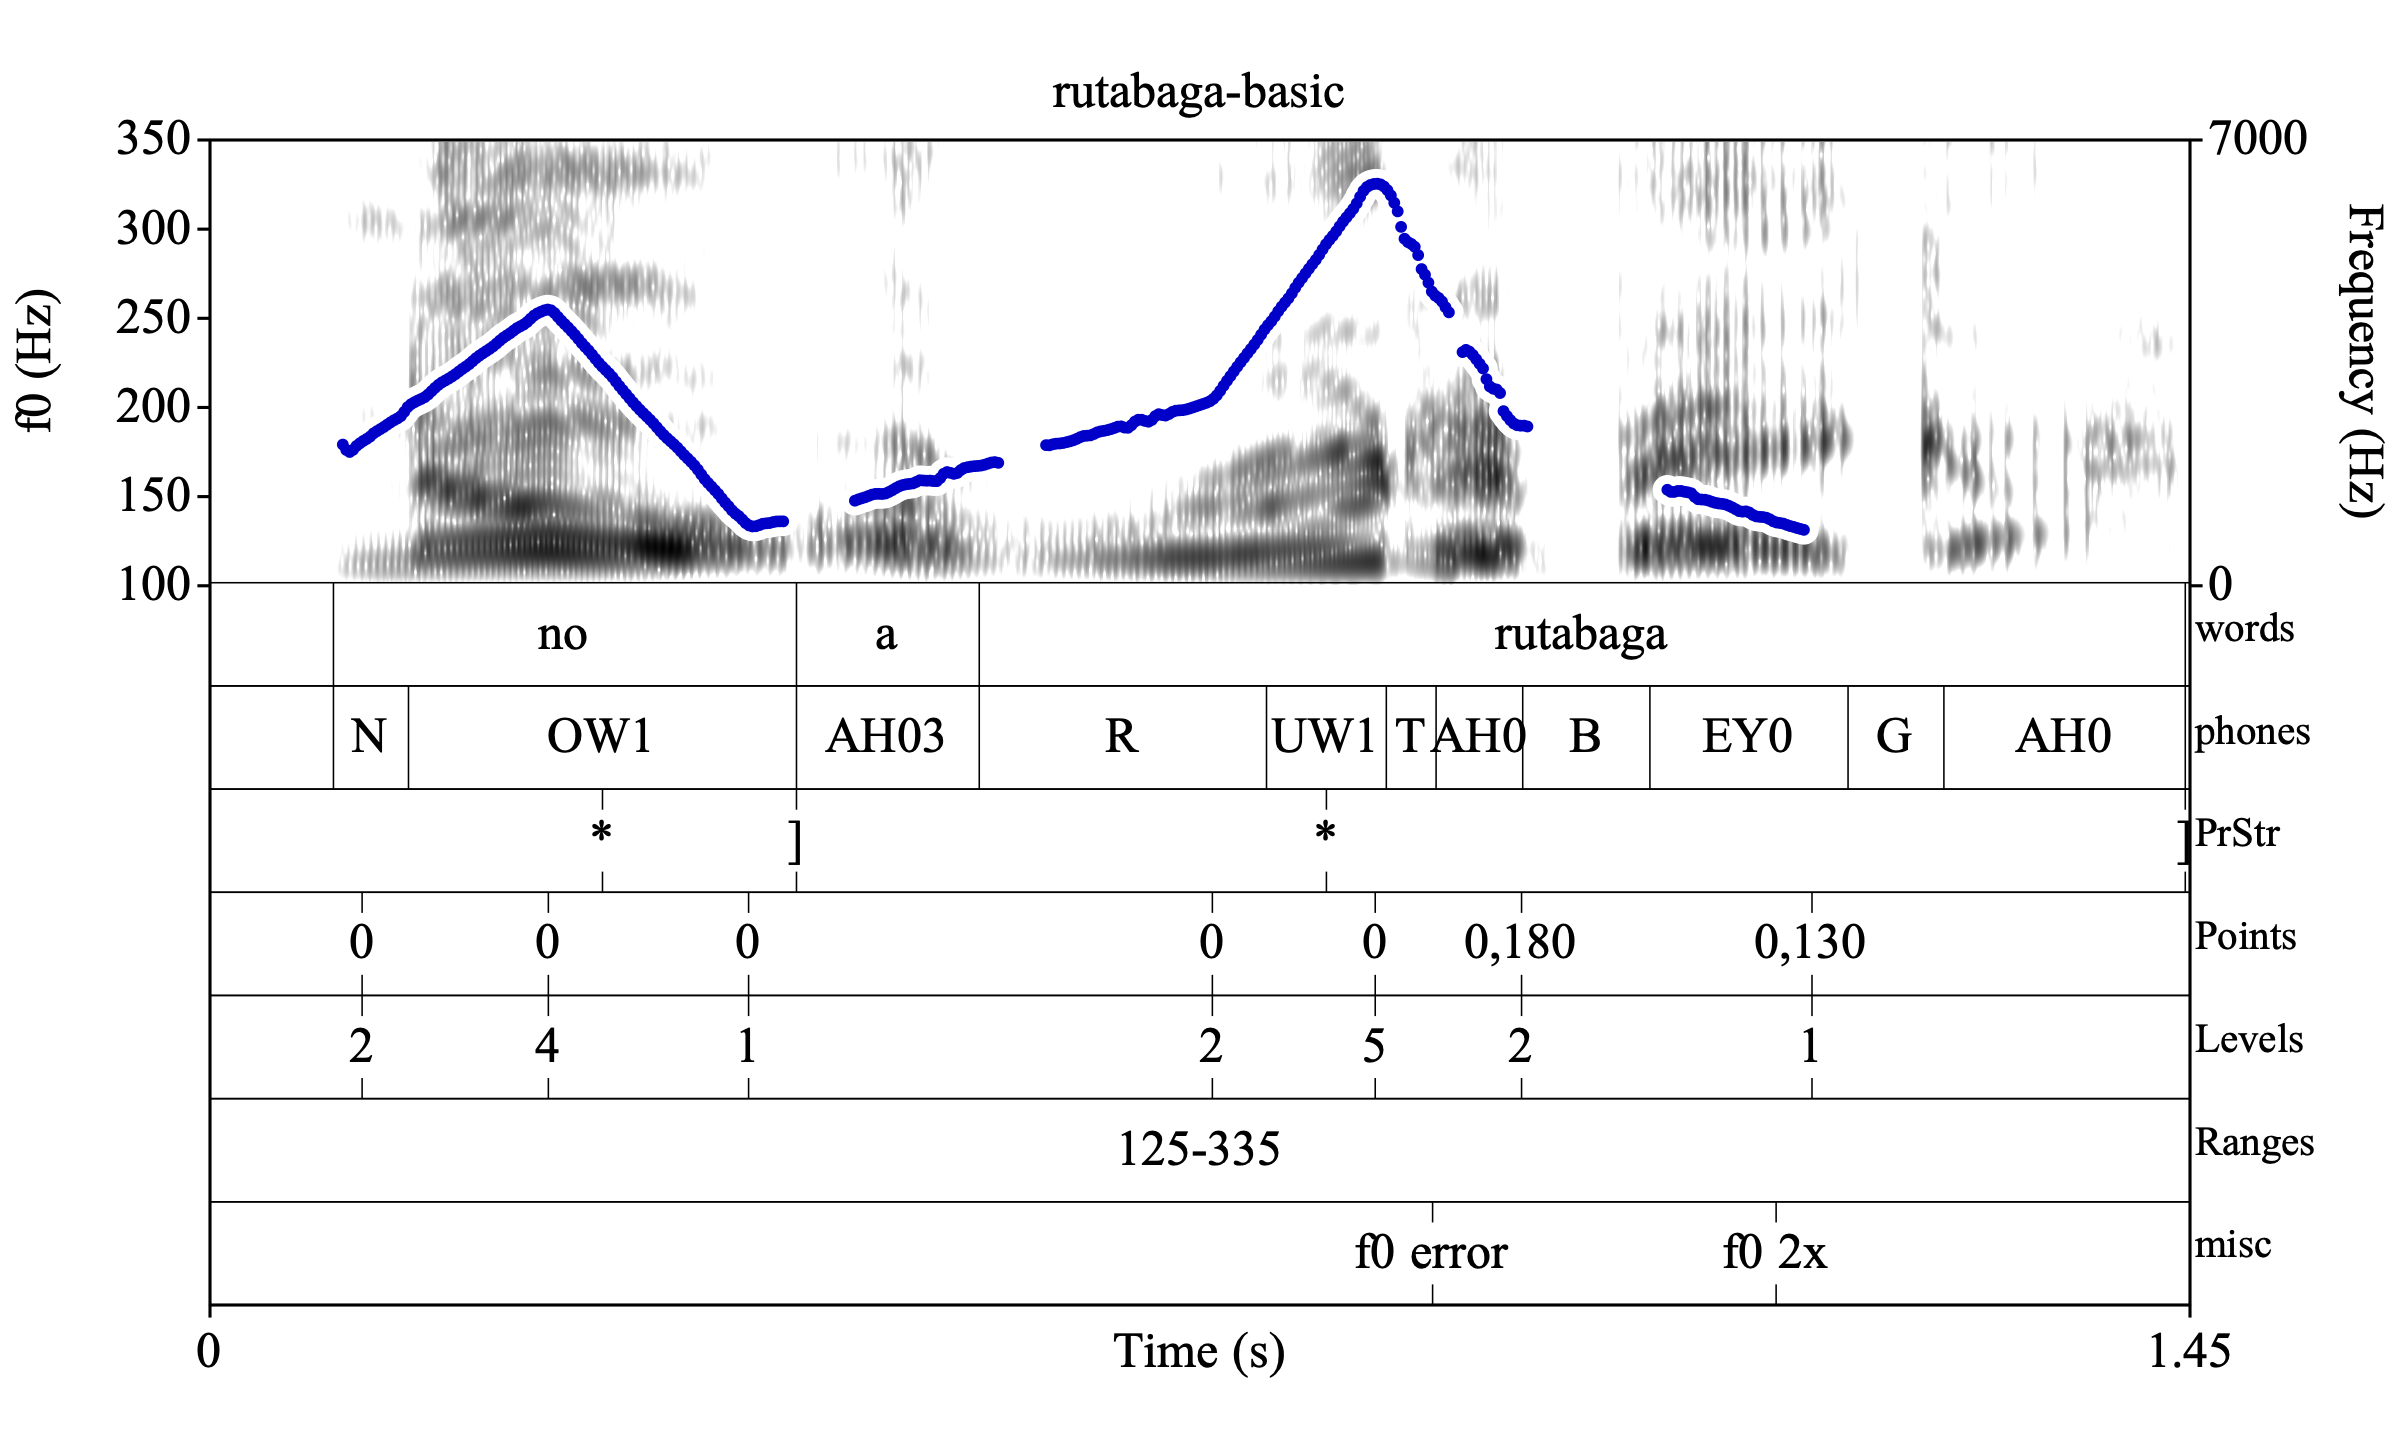
\includegraphics[width=.875\linewidth]{Contours-rutabaga-basic-resynth.png}
%
\caption{A resynthesis that is perceptually equivalent to the original that exhibited pitch doubling.%
\label{fig:rutabaga-resynth f0-tracking}%
\index{Annotated example, f0 tracking!rutabaga}%
}
\end{figure}

In the coming sections, we discuss some common sources of f0 tracking disruptions, that are due to the speech signal itself (and not the software or its settings).

\subsubsection{Segmental effects}\label{sec:segmental-effects}

Another very common set of cases where adjusting software settings may do enough to yield a clean f0 track have to do with the nature of the phonetic characteristics of certain speech sounds. (As noted earlier, these segmental effects are also known as “microprosodic” effects.) Because f0 tracks rely on regular and identifiable repeating patterns in the speech signal, and because speech sounds vary with respect to these properties, the f0 track is frequently influenced by the segments themselves. Some of the core types of segmental effects on f0 tracks are listed here:

\begin{itemize}
\item Voiceless segments: i.e., segments during which there is at least an interval where there is no vocal fold vibration. These are the most straightforward interruptions of the pitch track.
\item Distortions of f0 in the vicinity of obstruents (stops and fricatives): bumps up or down in f0 at the transitions between a consonant and a neighboring segment, or during a voiced fricative
\item Intrinsic pitch of certain vowels: [i] has a higher intrinsic pitch, [a] has a lower one 
\item[] (\uline{HINT}: Sonorant sounds yield fewer segmental effects on pitch, because they involve the most regular and most easily identifiable acoustic patterns with respect to f0.)
\end{itemize}

Consider the example in figure \ref{fig:marmalade cake f0-tracking}, which has the same intonational contour overlaid on utterances with very different segments. The first portion of the recording, “\langtext{Mariana made the marmalade}”, is mostly smooth and steady, because it is primarily composed of sonorant sounds (except the [d] and [ð], where the pitch track is notably less reliable). On the other hand, the second portion of the recording, “\langtext{Jack baked the cake}”, is much less reliable: during the stops and affricates in this utterance, Praat is unable to detect f0. Thus this is an example where the intonational contours are essentially the same, while the f0 tracks are very different, due to segmental effects.

\begin{figure}[H]
\centering
%
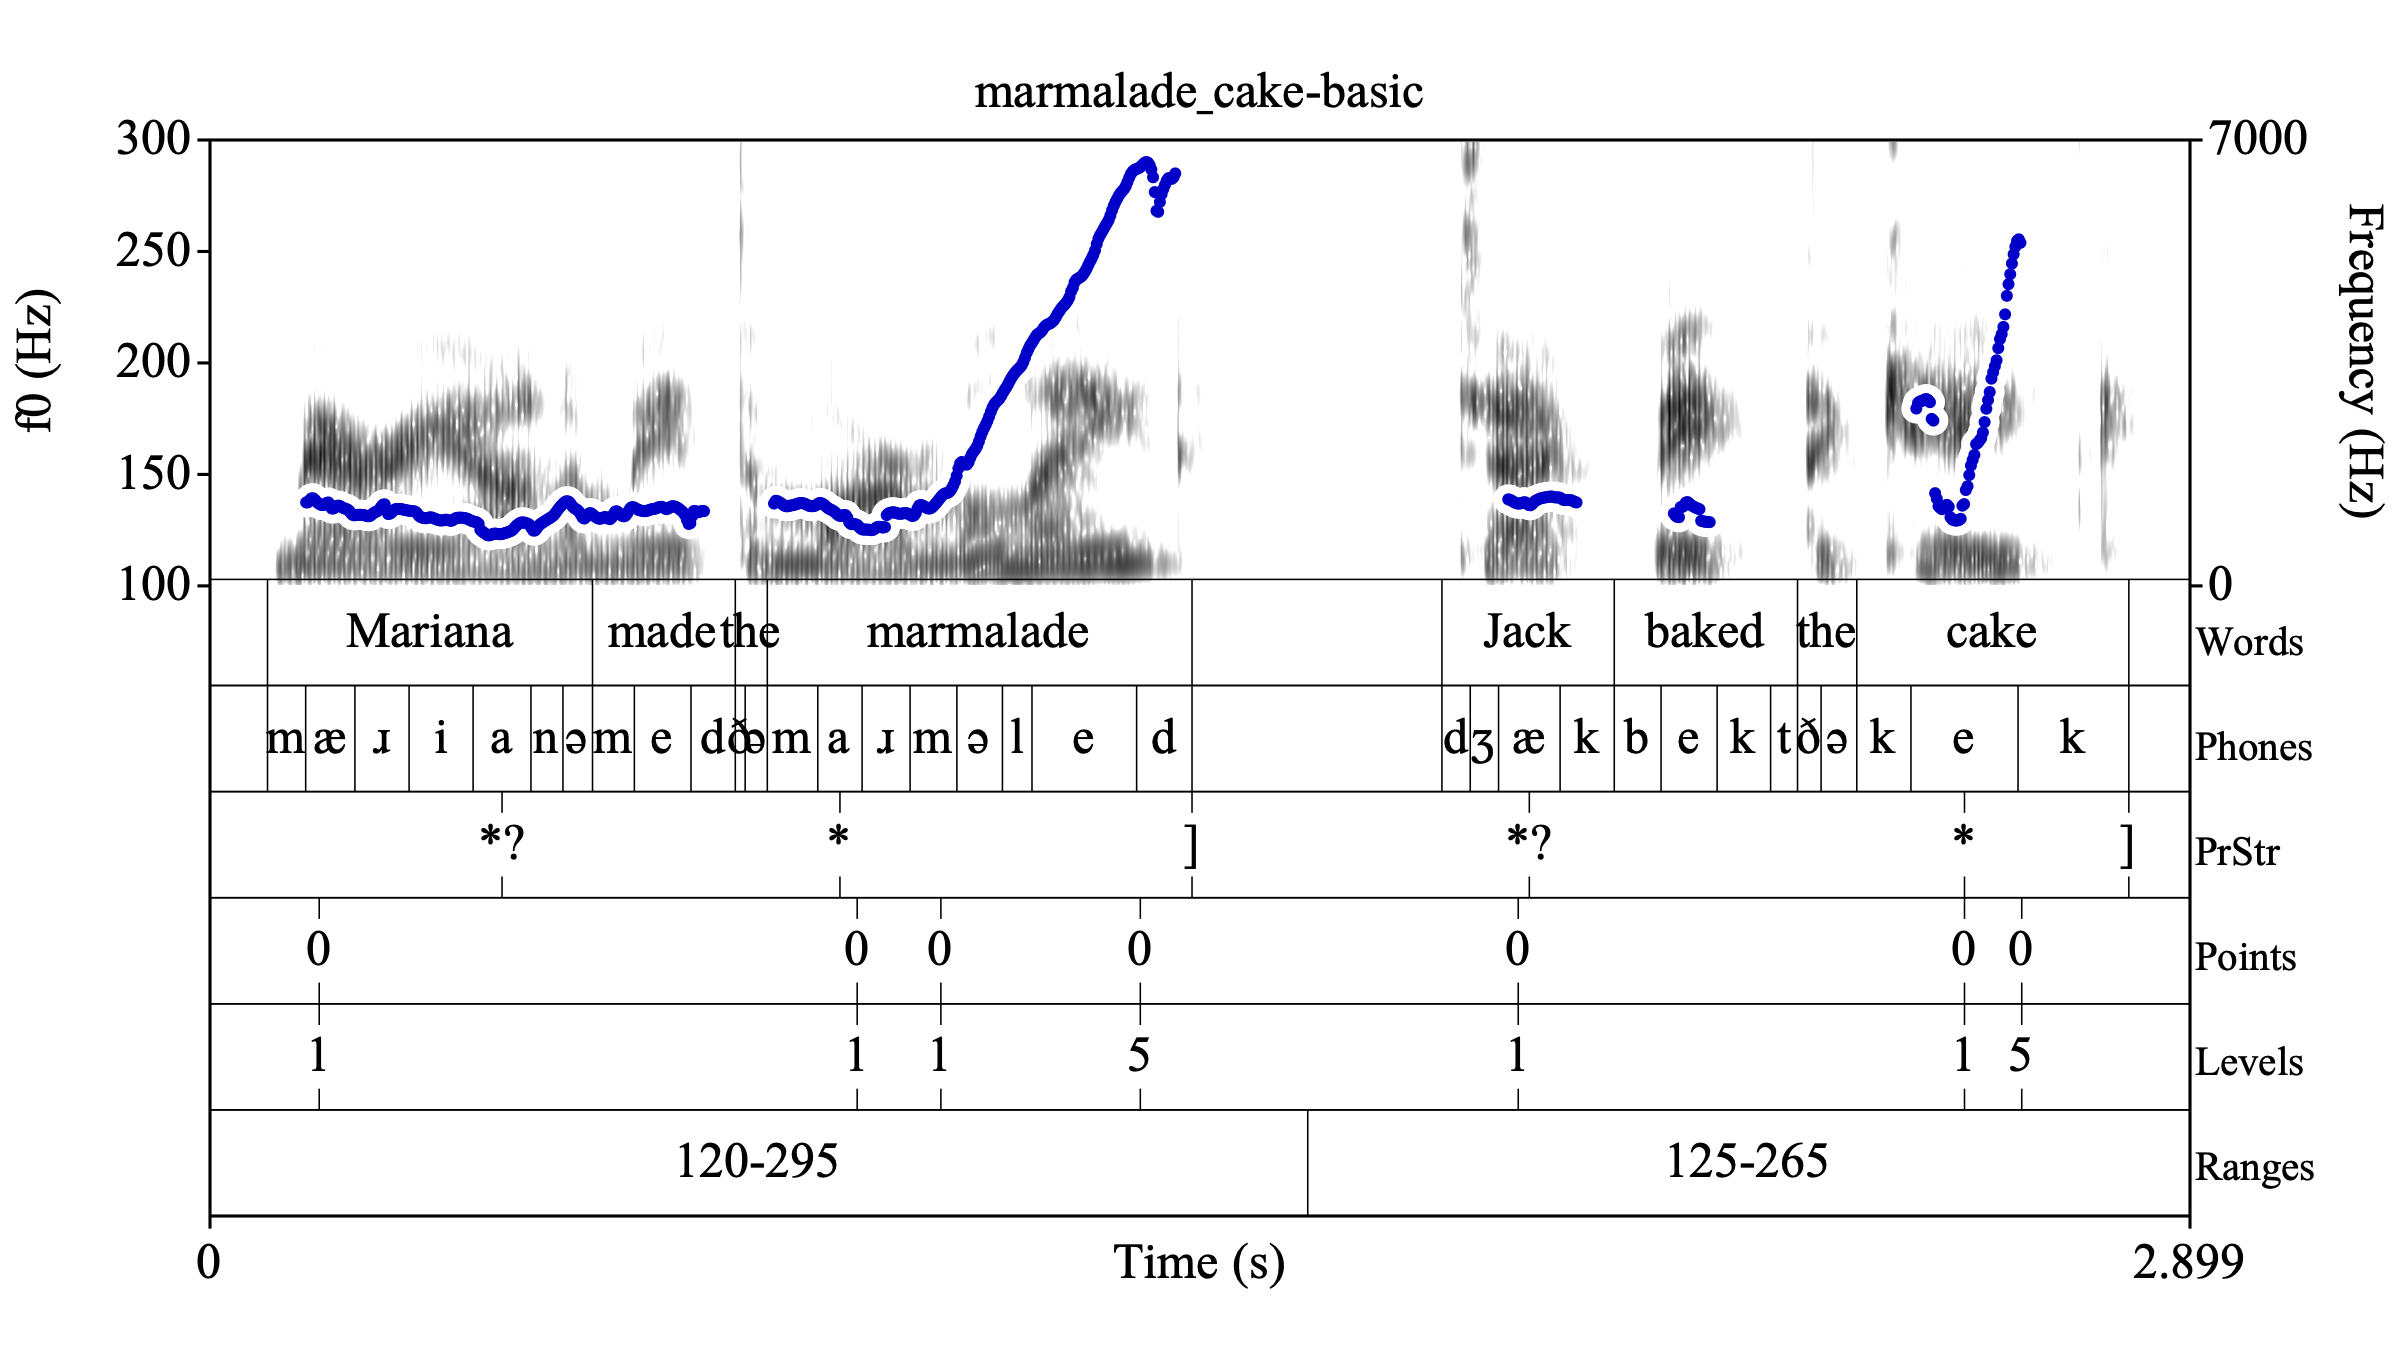
\includegraphics[width=.875\linewidth]{Appendix-marmalade_cake.png}
%
\caption{The same intonational melody applied to a sentence largely comprised of sonorant sounds (left) and to a sentence with many non-sonorants (right).%
\label{fig:marmalade cake f0-tracking}%
\index{Annotated example, f0 tracking!marmalade\_cake}%
}
\end{figure}

The example in figure \ref{fig:design improvements f0-tracking} shows additional examples where the f0 track is heavily distorted by non-sonorant sounds.  In particular, note that the [z] in “\langtext{design}” and the [mp] in “\langtext{improvements}” both cause a significant drops in the f0 track, but they do not correspond to drops in pitch – listening to this example, labellers perceive the pitch as rising steadily from the beginning of “\langtext{design}” to the peak in “\langtext{improvements}”, as reflected by the Points tier labels (which skip over the two mentioned drops in f0).

\begin{figure}[H]
\centering
%
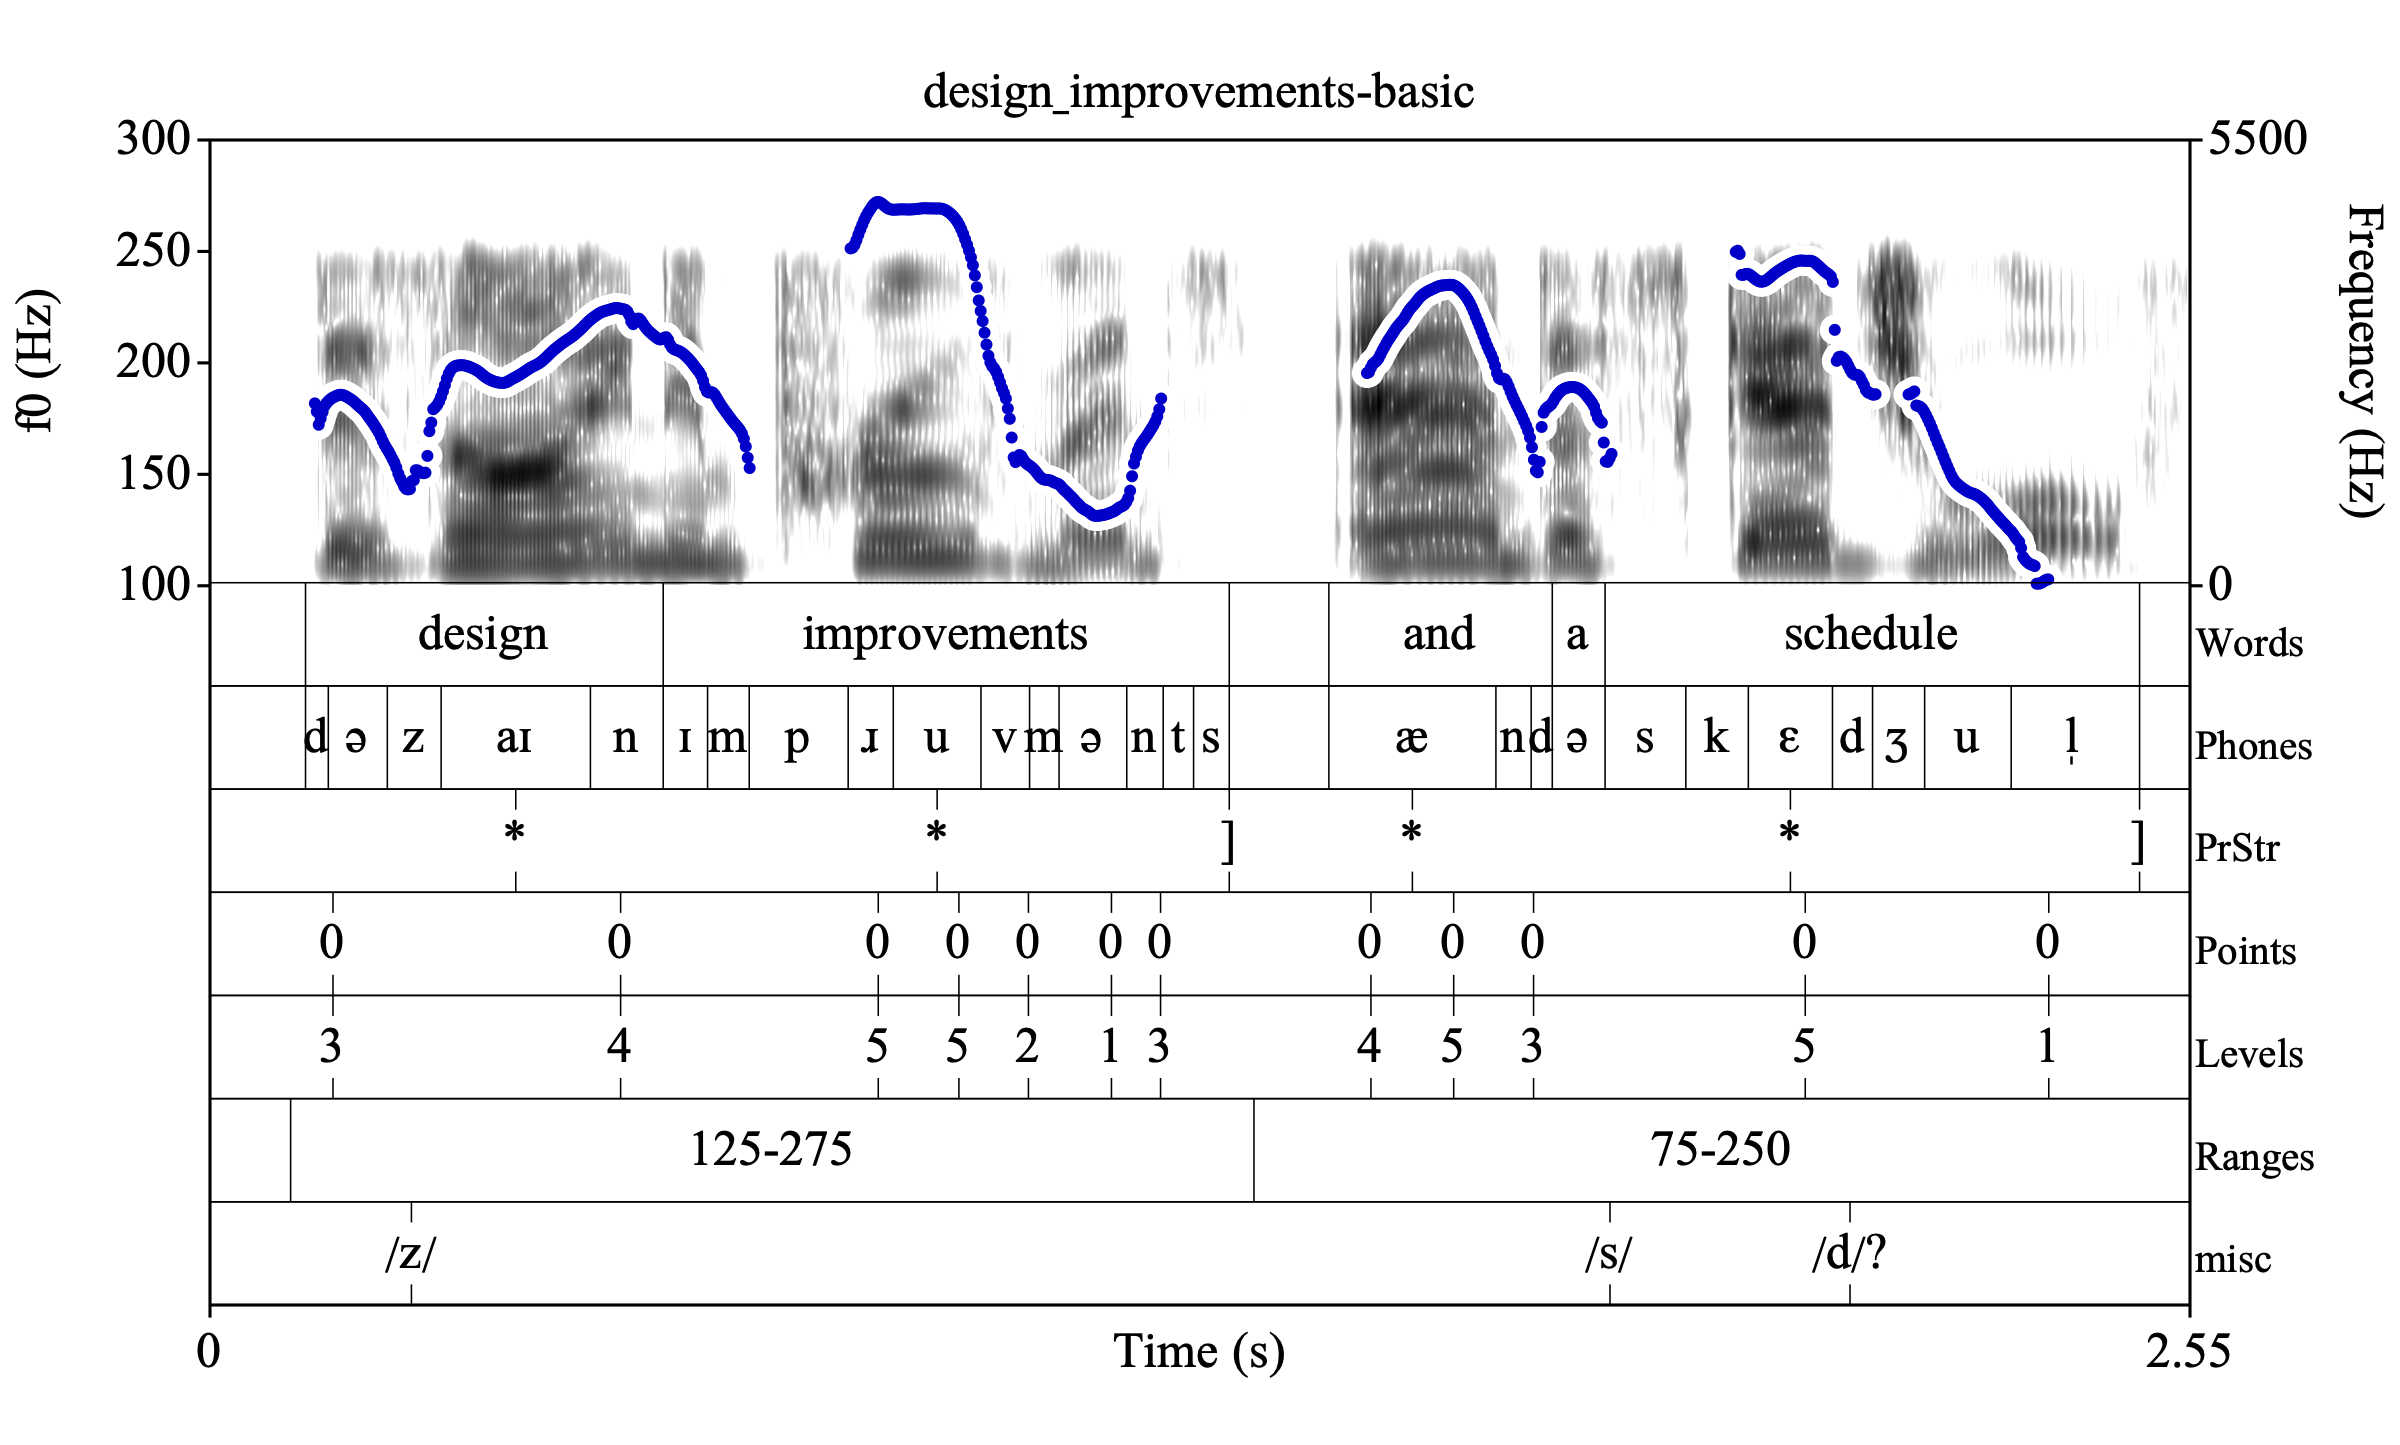
\includegraphics[width=.875\linewidth]{Appendix-design_improvements.png}
%
\caption{An example where non-sonorant sounds disturb the f0 tracking; this is especially noticeable in the [z] of “\langtext{design}” and [p] of “\langtext{improvements}”.%
\label{fig:design improvements f0-tracking}%
\index{Annotated example, f0 tracking!design\_improvements}%
}
\end{figure}

Consider now the example in figure \ref{fig:out of order-plateau f0-tracking}, which exhibits many small rises\slash falls in the f0 track. Note that the Points tier annotations reflect that the annotators perceive the pitch containing many fewer turning points – for example, the Points annotation reflects a mostly steady pitch during “\langtext{seems like it’s}”. This perception of much smoother pitch is reflected in the straight line approximation resynthesis in figure \ref{fig:out of order-plateau f0-tracking}.

\begin{figure}[H]
\centering
%
\includegraphics[width=.875\linewidth]{Appendix-out_of_order-plateau}
%
\caption{An example with lots of perturbations in the f0, due to segmental effects.%
\label{fig:out of order-plateau f0-tracking}%
\index{Annotated example, f0 tracking!out\_of\_order-plateau}%
}
\end{figure}


\begin{figure}[H]
\centering
%
\includegraphics[width=.875\linewidth]{Appendix-out_of_order-plateau-resynth}
%
\caption{A resynthesis on the basis of the Points annotation, to reflect the much smoother intonational contour that the annotator perceives.%
\label{fig:out of order-plateau f0-tracking}%
}
\end{figure}


\subsubsection{Voice quality effects}\label{sec:voice-quality-effects}
In addition to speech segments affecting how f0 is tracked, the voice quality of speech can also impact f0 tracking. (\uline{NOTE}: Voice quality effects —especially from creakiness— are especially common at the edges of prosodic groups.) Voice quality (a.k.a. phonation) refers to how the vocal folds (and the larynx more broadly) are configured during speech production. Modal voice (the “neutral” voice quality) does not impact f0 tracking, while other phonations such as creaky voice, breathy voice, and whisper voice can and do regularly impact f0 tracking. For example, during whispering or breathiness, the f0 track may be absent or values may appear somewhat scattered. 

A particularly frequent non-modal phonation is creaky voice; it is especially common at the ends of phrases and where the pitch is low. It is marked by irregular pitch periods and especially perceptual glottalization (which can be seen in a spectrogram as prominent vertical striations, as during the bulk of the final [i] in Fig. \ref{fig:joey f0-tracking}). During creaky voice, the f0 may disappear or appear to jump suddenly upwards\slash downwards. Both of these effects can be seen in Fig. \ref{fig:joey f0-tracking}: there is creaky voice during “\langtext{it to}” and at the end of “\langtext{Joey}”; during “\langtext{it to}” there is no f0 tracking, and during “\langtext{Joey}”, the f0 tracking jumps suddenly upwards (at the beginning of [i]) and then disappears until the speaker returns to modal voice at the end of the utterance.

\begin{figure}[H]
\centering
%
\includegraphics[width=.875\linewidth]{Appendix-joey.png}
%
\caption{Example of creaky voice phonation disturbing pitch tracking.%
\label{fig:joey f0-tracking}%
\index{Annotated example, f0 tracking!joey}%
}
\end{figure}

Another example of the impact of creaky voice on f0 tracking can be seen in Fig. \ref{fig:no_cigar f0-tracking}. From the beginning of “\langtext{but}” through the [n] of “\langtext{no}”, there is creaky voice during. During that time, there is no pitch tracking (even during the voiced [ʌ] and [n]), and when the f0 tracking returns, it appears to be high and falling onto the [o]; however, this f0 fall is due to the offset of creaky voice, and auditory perception indicates  that the pitch is steadily rising during “but no” (as reflected in Points labels). (Notice also that there are segmental effects from the [s] and [g] of “\langtext{cigar}".)

\begin{figure}[H]
\centering
%
\includegraphics[width=.875\linewidth]{Levels-no_cigar-basic.png}
%
\caption{Example of creaky voice phonation disturbing pitch tracking.%
\label{fig:no_cigar f0-tracking}%
\index{Annotated example, f0 tracking!joey}%
}
\end{figure}


\subsection{Guiding principles for recognizing and dealing with pitch track disruptions}\label{sec:guiding-principles-for-recognizing-and-dealing-with-pitch-track-disruptions}

\begin{enumerate} \def\labelenumi{\arabic{enumi}.}
\item If the f0 appears to change locally in a way that is surprisingly rapid and not clearly part of a bigger pitch pattern, consider the context in which those bumps, spikes or jumps are occurring. Could they be due to segmental effects or pitch tracking errors? Is the “pitch range” in the “pitch settings”
\item In PoLaR labelling, where possible, put Points labels at places in the signal where you believe that the f0 measured corresponds to the pitch you perceive at that region of the utterance
\item For places where you believe a point or range floor or ceiling occurs during unreliable pitch, estimate what the f0 value should be at that point. (See detailed guidelines in the Advanced Points labelling section.) \end{enumerate}